%!TEX TS-program = xelatex 

%!TEX encoding = UTF-8 Unicode
%
%  perception
%
%  Created by Mark Eli Kalderon on 2018-05-07.
%  Copyright (c) 2018. All rights reserved.
%

\documentclass[12pt]{book} 

% Definitions
\newcommand\mykeywords{perception, Plato, Timaues}
\newcommand\myauthor{Mark Eli Kalderon}

% Packages
\usepackage{geometry} \geometry{a4paper} 
% \usepackage{url}
% \usepackage{txfonts}
\usepackage{color}
\usepackage{epigraph}
% \usepackage{enumitem}
\usepackage{enumerate}
% \usepackage{tikz}
% \usepackage{amsmath}
% \usepackage{tkz-euclide}
% \usetkzobj{all}
\definecolor{gray}{rgb}{0.459,0.438,0.471}
% \usepackage{setspace}
% \doublespace % Uncomment for doublespacing if necessary

% XeTeX
\usepackage[cm-default]{fontspec}
\usepackage{xltxtra,xunicode}
\defaultfontfeatures{Scale=MatchLowercase,Mapping=tex-text}
\setmainfont{KoufrUni}
\newfontfamily{\sbl}{SBL BibLit}

% Bibliography
\usepackage[round]{natbib}

% Index
% \usepackage{makeidx}
% \makeindex

% PDF Stuff
\usepackage[plainpages=false, pdfpagelabels, bookmarksnumbered, backref, pdftitle={Form Without Matter}, pagebackref, pdfauthor={\myauthor}, pdfkeywords={\mykeywords}, xetex, colorlinks=true, citecolor=gray, linkcolor=gray, urlcolor=gray]{hyperref}

%%% BEGIN DOCUMENT
\begin{document}

% % Title Page
\author{\myauthor}
\title{Timaeus on Sense and Sensibilia}
\date{}

\maketitle
\pagenumbering{gobble}
\frontmatter
%!TEX root = /Users/markelikalderon/Documents/Git/timaeus/timaeus.tex
\epigraph{The development of consciousness in human beings is inseparably connected with the use of metaphor. Metaphors are not merely peripheral decorations or even useful models, they are fundamental forms of our awareness of our condition: metaphors of space, metaphors of movement, metaphors of vision.}{Iris Murdoch, \emph{The Sovereignty of Good}}
\epigraph{Due to being confused here, I have become a seeker of the secret.}{Farīdu'd-Dīn `Aṭṭār, \emph{Manṭiqu'ṭ-Ṭair}}
\pagenumbering{roman}
\tableofcontents
%!TEX root = /Users/markelikalderon/Documents/Git/timaeus/timaeus.tex
\chapter*{Preface} % (fold)
\markboth{\MakeUppercase{Preface}}{}
\addcontentsline{toc}{chapter}{Preface}
\label{cha:preface}

The books on Plato are legion. It is with some reluctance that I add to the heap. I thus feel obliged to provide some reason for doing so. Whether, in the end, I had sufficient reason is for the reader to decide.

I have long been interested in extramission theories of visual perception for which Empedocles' lantern analogy (Aristotle, \emph{De sensu} 2 437b27–438a3 = DK 31B84) and the Timaean account of vision (45b–46c, 67c–68d) that it inspired are important sources. In the current naturalistic climate, this is an unfashionable interest, since extramission theories provide manifestly false causal models of visual perception. However, my interest in extramission theories is less with the causal model they provide for vision, than what phenomenological insights they may retain despite providing such models. For they make vivid the active outward directionality of vision, and I felt that it was important to recover whatever insights they may afford into this aspect of visual phenomenology \cite[see][chapter 5, for an initial attempt]{Kalderon:2018oe}. A proper understanding of Timaeus' account of vision is an essential step for such a project.

Partly for ideological reasons, I have a broader interest in the premodern history of the philosophy of perception. I believe that contemporary philosophy of perception is hampered by assumptions inherited from early modern philosophy. Much of modern philosophy of perception still works within the modern paradigm, even the work of philosophers who self-consciously seek to go beyond it. Thinking hard about premodern philosophy of perception is a much needed propaedeutic in the search for alternatives. Timaeus' account of visual perception plays a crucial role in thinking about visual perception in both classical antiquity and the Hellenistic period (see \citealt[chapter 1]{Lindberg:1977aa}). A proper understanding of Timaeus' account of vision is an essential step, as well, for this broader project.

My interest in the Timaeus was not limited to vision, however. Timaeus provides accounts of the five special senses, if I may help myself here to this Peripatetic anachronism. And even if one were exclusively interested in Timaean vision, no adequate understand of vision as Timaeus conceives of it is possible by exclusively focussing on the two passages where Timaeus discusses vision (45b–46c, 67c–68d). Thus, for example, an important general claim about the aetiology of perception only emerges in Timaeus account of pleasure (64a2–65b3), and as \citet{Barker:2000dy} and \citet{Lautner:2005aa} argue, Timaeus account of audition has implications for his general understanding of perception. Moreover, I have been moved by the emerging general consensus in the philosophy of perception that it is a mistake to focus on vision to the exclusion of the other senses and so welcomed the opportunity to closely examine Timaeus' general survey of these.

Not only is my discussion of the \emph{Timaeus} not limited to the account of vision, neither is it limited to the passages that explicitly discuss perception more generally. Even a narrow focus on perception will reveal that the providence of the benevolent Demiurge is not completely understood without detailed knowledge of the workings of the liver. Indeed no major part of the Timaeus' speech is without direct relevance to the nature of perception as Timaeus conceives of it. The proemium, the cosmogony, the psychogony, the discussion of the mortal soul and the flesh that contains it, no less than Timaeus' discussion of auxiliary and true causes of vision and audition and the affections common to the body as a whole and peculiar to particular parts of the body in giving rise to perception and sensation, are all directly relevant. Conversely, perception, a specialist interest, assumes a cosmic significance in Timaeus' system. At first this occasioned despair. Short of writing a linear commentary on the entirety of Timaeus speech, which threatened to be of comparable length to Proclus' own monstrously long commentary, how could one manage this material? Nevertheless, I persisted and somehow muddled through, hopefully not producing a muddle in the process.

In thinking about the Timaeus, I have relied on a variety of different sources. While \citet{Skemp:1942oc} is surely right that an understanding of Timaeus' pre-Socratic sources is relevant to understanding the positions he develops, it seems odd to restrict oneself to these. Skemp himself relies on the works of the great British commentators, Archer-Hind, Taylor, and Cornford. But if one can help oneself to the insights of these, why not also help oneself to whatever insights might be afforded by Plutarch, Calcidius, and Proclus? Or Aristotle and Theophrastus, not to mention Pseudo-Timaeus Locri? As an initiate, it seemed audacious of me to ignore these important contributions to our collective understanding. And throughout, I have relied not only on these but on the work of art historians, medical historians, classicists, as well as historians of ancient philosophy. As I had no idea what I was doing when I began, I couldn't very well ignore any help provided, no matter its source.

As I wrote the present essay, I experimented with different ways of organizing the material. My initial thought was to organize the material by following the causal process that eventuated in perception. I experimented as well with other schemes. I found that I could follow none of them to the end. With each departure from Timaeus' presentation I eventually found my thoughts curbed or hampered in some way. I came to have a deep appreciation for the care and insight with which Timaeus organizes and presents his cosmology in a way that I would not had I not fought so hard against it. In the end, then, I have largely followed Timaeus' lead. This too has its drawbacks. Promissory notes must be issued and made good later on in the narrative. The discussion thus oftentimes loops back and picks up on earlier threads. Perhaps this is a manifestation of Plato's intent to provoke his audience to actively engage with the text. I confess that I often entertained doubts about whether I was up to this task. I am not sure that I have completely allayed these doubts. My greatest hope is that, at least in some small way, I have facilitated Plato's intent, that the present essay may itself provoke the reader to actively engage with the \emph{Timaeus}. It is not for nothing that Raphael depicts Plato as holding that book in his fresco \emph{Scoula di Atene} in the \emph{Stanze di Raffaello} in the Apostolic Palace.

Theophrastus in reporting the accounts of sense and sensibilia found in the \emph{Timaeus} straightforwardly attributes these to Plato (\emph{De sensibus}), and \citet{Cornford:1935fk} follows him in this. \citet{Taylor:1928qb}, by contrast, denies any such an attribution. Rather, he took Plato to be reporting the distintively Pythagorean views of Timaeus. Taylor's interpretation has been criticized by Cornford. Despite the merits of Cornford's case, I do not believe that we are thereby licensed to follow Theophrastus in straightforwardly attributing Timaeus' views to Plato. Throughout, I have focused on Timaeus' views quite apart from the question of whether or not, or to what extent, they may be attributed to Plato. Indeed, doing so, is, I believe, an essential first step in determining the relation between Timaeus' views and Plato's. Thus I make limited use of the broader Platonic corpus. If the views of Timaeus are compared to views that emerge in other Platonic dialogues, this is not done for the sake of establishing what Plato really thought. Such comparisons may reveal, for example, what is distinctive about Timaeus' development of a view. So for example, Timaeus has a distinctive take on the tripartite psychology, emphasizing its anatomical aspect.

To understand perception's cognizance of its object, on must understand Timaeus' general account of cognition. Timaeus associates cognitive activity with circular motion. Ever since Burnyeat's Cambridge seminar on the \emph{Timaeus}, there has been a growing trend to interpret such motion literally. This is in sharp contrast with the great British commentators who, influenced by the neo-Platonists, were inclined to offer non-literal interpretations of various aspects of Timaeus' speech. 

There are many salutary aspects of the literalist trend. Formost among these, to my mind at least, is the way that a literalist interpretation forces us to focus on the oftentimes unruly details of Timaeus' speech. However, this is sometimes conflated with the more general precept that to take an account seriously one must understand it literally \citep[see][7]{Broadie:2012vl}. Something like that precept is accepted both by the literalists and many of their opponents. Indeed, some of the latter refuse to take seriously certain aspects of Timaeus' account and so offer non-literal interpretations of it.

The general precept is false. Metaphor is not, or not merely, a device of non-commit\-ment. Nor is it merely ornamentation. Nor is metaphor everywhere dispensable. To think otherwise is to ignore the important role metaphors play in our cognitive lives. Adherents of the general precept, be they literalist or not, are blind to the cognitive content of metaphorical thought. Ironically it was following the lead of the literalists and focusing on the details of Timaeus' speech that convinced me that a literal interpretation of the soul's motion is impossible. Literalists, such as \citet{Sedley:1997kr}, can take seriously, and so literally, certain aspects of Timaeus' speech, but as we shall see, only by ignoring others. Specifically, Timaeus offers two spatial descriptions of the World Soul that conflict. Attending to one description and not the other masks that conflict. Worse still, not only do these spatial descriptions conflict, but each are self-contradictory or otherwise internally incoherent (chapter~\ref{cha:psychogony}). If that is right, then there is no question of interpreting the spatial attributes of the soul literally. And, hence, no question of interpreting the motion of the soul literally. Taking the association of cognitive activity and circular motion seriously requires that we understand circular motion as a metaphor for cognitive activity (chapter~\ref{cha:cognitive_revolution}). 

This approach was fruitful with respect to other aspects of Timaeus speech as well. Thus, for example, Timaeus deploys a weaving metaphor for the union of soul and body. Attending to textile archaeology and the religious significance of weaving in the festivities of the Panathenea allow us to understand that metaphor and so better understand the soul-body union as Timaues conceives of it. Careful attention to metaphor also sheds light on the moral significance of Timaean anatomy, too often overlooked by modern commentators (\citealt{Steel:2001ay} is a notable exception).

My staunch opposition to literalism is not an expression of ingratitude. It is only because I have learned so much from scholars defending literalism that I have been emboldened to criticize their views.



% Chapter preface (end)
%!TEX root = /Users/markelikalderon/Documents/Git/timaeus/timaeus.tex
\chapter*{Acknowledgements} % (fold)
\markboth{\MakeUppercase{Acknowledgements}}{}
\addcontentsline{toc}{chapter}{Acknowledgements}
\label{cha:acknowledgements}

Thanks to Justin Broackes for a conversation in Cambridge about \emph{diaphanē} in Aristotle which I found fruitful in application to the Timaean account of transparency.

% chapter acknowledgements (end)

\mainmatter

%!TEX root = /Users/markelikalderon/Documents/Git/timaeus/timaeus.tex

\chapter{\emph{Proemium}} % (fold)
\label{cha:proemium}

\section{A Double Significance} % (fold)
\label{sec:a_double_significance}

The first part of Timaeus's speech is traditionally called the \emph{proemium}, echoing Socrates' own description of it at 29d5 as \emph{prooimion} or prelude. Entitling the present chapter ``\emph{Proemium}'' thus has a double significance. It at once announces that the present chapter will take Timaeus' \emph{proemium} as its subject matter and that the chapter will itself serve as prelude to the essay as a whole.

% section a_double_significance (end)


\section{\emph{Proemium}} % (fold)
\label{sec:proemium}

The \emph{proemium} is bounded by the last two remarks that Socrates will make in the dialogue. In the first, just prior to Timaeus speaking, Socrates praises the feast of \emph{logoi} that has been proposed as a return gift for his speech the previous day on the topic of the \emph{Republic} and prompts Timaeus to begin by duly invoking the gods. In the second, Socrates praises Timaeus, accepting his prelude, and encouraging him to proceed. In the \emph{proemium}, Timaeus begins by invoking the gods. After which Timaeus states some general principles, which he uses to circumscribe his subject matter and describe the kind of account that he proposes to give of it. 

The principles include:
\begin{enumerate}[(1)]
	\item The distinction between that which always is and has no becoming and that which becomes and never is and the manner in which they are cognized
	\item The principle that everything that has come to be has a cause
	\item The principle that the cause of that which has come to be is a maker that looks to a model
	\item The principle that if that which has come to be and never is is beautiful then it has been modeled on that which always is and has no becoming by a good maker
\end{enumerate}

That which always is and never becomes is the object of understanding (\emph{noēsis}) based on reasoning (\emph{logos}). That which becomes and never is is the object of opinion (\emph{doxa}) based on unreasoning perception (\emph{aisthēsis}). That which always is and has no becoming is intelligible, and that which becomes and never is sensible. The Cosmos is sensible and thus must belong to the realm of Becoming. That which becomes and never is has a cause. This causes is a maker that looks to a model. Since the Cosmos is beautiful then by the final principle, Timaeus concludes that the Cosmos has an intelligible model and a good maker. It is the generation of the Cosmos, conceived as a beautiful likeness of an intelligible model, that will be the subject matter of Timaeus' speech. Accounts should be appropriate to their subject matter, and Timaeus concludes that since his subject matter is a likeness his account shall be ``likely''.

While the general outline of the \emph{proemium} is relatively clear, each element of this tightly constructed account requires comment as does their interrelation. 

% section proemium (end)

\section{The Invocation of the Gods} % (fold)
\label{sec:the_invocation_of_the_gods}

Timaeus invokes the Gods, and his prayer is addressed to the Gods invoked. Without dwelling overmuch on Timaean theology, two remarks are worth making about Timae\-us' invocation of the Gods. The first is an observation about who is not invoked, and the second is a puzzle about who is invoked.

It is reasonable to call upon God at the outset of an undertaking. This is presented as a general practical precept. Later Timaeus explains that we invoke the Gods so as to pray for their approval of our undertaking. It would be unreasonable to fail to do so. And this remains so whether the undertaking is great or small. Timaues, however, proposes to undertake an account of the All (\emph{toū pantos}---understood, here, as the Cosmos without the explicit suggestion that it is ordered) and whether and how it was generated. This is a grand topic and a great undertaking so it is especially appropriate that Timaeus call upon the Gods at the outset.

What it is to pray for such a great undertaking is elaborated in Timaeus' final prayer (\emph{Critias} 106a1–b6). There Timaeus prays that his words may endure if they are spoken truly and meet with divine approval. Timaeus further prays that should his speech be false that a just penalty be imposed, the just penalty in the case of error being correction. Finally, Timaeus prays for knowledge, the most perfect among medicines, so that he may speak truly in the future.

It is striking who is not called upon by Timaeus. Notable in His absence is the Demiurge, the Maker and Father of the All. The Maker and Father of the All is difficult to discover and impossible to explain to everyone (28c3–5). He only begins to emerge in reasoning from principles that Timaeus only states after the invocation. Timaeus is invoking the Gods and addressing his prayers to Them, in part, in aid of this difficult discovery. If so, then the object of his search was not among the Gods that were invoked even it is itself divine.

There is a related reason for thinking that the Demiurge was not among the Gods invoked and prayed to. Even if it were possible to privately invoke the Gods and pray for their approval of some solitary undertaking, this is not the context that Timaeus finds himself in. The invocation of the Gods urged by Socrates was, importantly, a public act of piety. And Timaues complies in the first person plural. It is we who are about to converse that have need to invoke the Gods and the Goddesses. A divinity difficult to discover and impossible to explain to all is perhaps not the most apt choice to invoke in a public act of piety. One's piety toward the difficult to discover divinity may be genuine but it might not be publicly manifest. One's piety is only guaranteed to be publicly manifest if directed toward recognized divinities. And a difficult to discover divinity impossible to explain to all is not a recognized divinity. The obscurity of the Maker and Father of All is inconsistent with the public nature of the invocation.

Perhaps, in the present instance, the public is restricted to the divided reference of ``we''---Timaeus, Socrates, Critias, and Hermocrates. The restriction may be significant. A divinity not widely known to many may yet be known to the present few. However, while Timaeus might rely on Socrates to already know of this difficult to discover divinity, is it really reasonable that Timaeus should similarly rely on Critias? Even among the present dignitaries, the obscurity of the divinity is in tension with the publicity of the act.

As \citet[13--4]{Broadie:2012vl} observes, the Demiurge is not invoked in any of the prayers offered by Timaeus. Broadie's observation coheres with the present explanation. Since all of the prayers in the dialogue are public acts, the obscurity of the divinity would preclude His public invocation.

Not only is it notable that Timaeus does not invoke the Demiurge, but it is obscure who is being invoked. Specifically, is Timaeus invoking one God or many? Notice he first calls upon God in the singular and then upon Gods and Goddesses in the plural. When Timaeus first calls upon God in the singular, it is in stating the general practical precept to call upon God and pray for approval of one's undertaking. When Timaeus calls upon Gods and Goddesses in the plural, this is not in the context of stating a general practical precept, but rather in the context of proposing to undertake an account of the All and its generation. Perhaps it is the Young Gods who are being invoked when Timaeus invokes the many. The Young Gods are divine, immortal beings generated by the Demiurge who are the instruments of Demiurgic activity. Specifically, as we shall see (chapters~\ref{cha:incarnation} and \ref{cha:the_flesh_and_the_mortal_soul}), they play an indispensable role in the generation of mortal beings. If the Young Gods are the many, who could the one be if not the Demiurge? One candidate is the All itself. Timaeus conceives of the Cosmos as a visible God (34a8, 34b8--9, 92a5--9), defers to it concerning its proper name in act of ritual piety (28b3--5, for discussion see \citealt[66]{Taylor:1928qb}), and addresses his final prayer to that God (\emph{Critias} 106a1--b6). By contrast, as \citet[35]{Cornford:1935fk} observes, ``Neither in the \emph{Timaeus} nor anywhere else is it suggested that the Demiurge should be an object of worship: he is not a religious figure.''

There are, of course, alternatives. Perhaps the God in the singular being invoked is a generic divinity of which the Gods and the Goddesses in the plural are species. On this alternative, an appeal to a generic divinity is appropriate in the statement of the content of a general practical percept. Similarly, it is appropriate to invoke the species of this generic divinity given the specific undertaking to account for the All. That all species of divinity should be invoked and their approval prayed for is perhaps only required for their specific undertaking of discoursing on the All and its generation. Perhaps a single divinity would do if the undertaking were small enough. But the collective undertaking that Timaeus proposes is suitably grand as to require the invocation of every species of divinity.

A deflationary take on the identity of the Gods invoked might might be motivated by the perfunctory nature of the invocation. Proclus describes the worry as follows:
\begin{quote}
	But how can it be, they say, that Timaeus has announced with a grand flourish that one should pray and call on the gods and goddesses, but that he fails to do this himself and immediately turns to proposed accounts without praying? (Proclus, \emph{In Timaeum} 1 221.9--12, \citealt{Diehl:1903re}; \citealt[58]{Runia:2008aa})
\end{quote}
If Timaeus has not in fact prayed, then there is no point in inquiring into to whom Timaeus has addressed his prayer. (That the invocation of the Gods should strike some as a grand flourish is worth remarking on. As \citealt[104]{Runia:1997vz}, observers, ``Only a minority of \emph{prooemia} begin with an \emph{invocation of the gods}, continuing in the tradition set by Hesiod in his \emph{Theogony}.'') Proclus' reply is ingenious in that he, in effect, proposes that we understand Timaeus' speech as performative in something like Austin's \citeyearpar{Austin:1975nx} sense. In saying that we must pray to the Gods, Timaeus has done just that. While one may decide to pray and pray later, in true prayer, the decision to pray and prayer are one and the same thing. Timaeus's public prayer on the occasion of the Panathenaea is a true prayer. And so in saying that we must pray, he does.

Still, exactly who is being invoked by Timaues may not be so neatly resolvable. Perhaps there is a kind of semantic slippage here, from singular to plural, the one resolving into the many. If so, this will be echoed in the third part of Timaeus' speech which concerns the interaction of Reason and Nececssity, especially in his account of the generation of the flesh and the mortal soul. There, Timeaus slides freely between singular and plural in describing what is officially meant to be rational cooperative activity, the Demiurge generating the immortal part of the soul and the Young Gods weaving it together with its mortal body that they generated from corporeal material borrowed from the body of the Cosmos. However, even for tasks that are meant for the Young Gods, their executions are sometimes described in the singular. We shall discuss the significance of this when we discuss the flesh and the mortal soul (chapter~\ref{cha:the_flesh_and_the_mortal_soul}). For now, I merely note a potential anticipatory trace of this puzzling usage. 

One last observation. Not only are the Gods invoked, but Timaeus also invokes themselves. The plural self-invocation is for the audience---Socrates, Critias, and Herm\-ocrates---to more easily learn and for the speaker---Timaeus---to more clearly expound his account of the All and the cause of its generation. (On the self-invocation see Proclus, \emph{In Timaeum} 1 222.11--223.2, \citealt{Diehl:1903re}.) Not only is Timaeus praying for the approval of the Gods concerning their present collective undertaking---his conversing with them about the nature and generation of the All---but he is importantly also praying that they themselves approve of their discourse, if only after being granted divine approval. While for the most part, Timaeus delivers an uninterrupted speech, in the invocation he describes it as a collective activity with the audience as co-participants. Perhaps the self-invocation is meant to get the participants of the discourse in a position where they may engage in it in such a way that they come to themselves approve of that discourse. This would involve the audience rationally attending to the speaker's account so that they may more easily learn his views about the nature and generation of the All. And this would involve the speaker clearly expounding his views to this audience. Even if largely a monologue, Timaeues' speech remains directed to its audience. And Timaeus must bear them in mind if he is to clearly expound his views to them in such a way as warrant their collective approval. Only in this way could the return speech discharge Timaeus' obligation to Socrates. Notice that it is his views that Timaeus wishes his audience to learn. Contrast learning the truth about the All and its generation. Timaeus is pointedly not proposing to demonstrate such truths. Timaeus, here, is quietly allowing room for what will emerge as accounts with a specific epistemic status, ``likely'' accounts.

If the plural self-invocation still seems odd or unfamiliar, it really should not. You have doubtless encountered it in contemporary speech. Think of someone inaugurating their address with ``Let's do this!'' Think of a motivational speaker or, better yet, a Hip Hop artist. ``This'', that which is to be done (dropping bars for the Hip Hop artist, cosmology for Timaeus, both are \emph{logoi}), is explicitly represented as a collective activity---``Let \emph{us} do this'', where ``us'' includes both speaker and audience. In saying ``Let's do this!'', the speaker draws attention to themselves, making their audience more receptive to their address, and the speaker expresses their determination in a way that draws the speaker's own attention to their audience, in an attempt to thereby more effectively deliver their address. Should the speaker prove genuinely effective, they may even garner approval for that address. It even has, in line with Proclus' suggestion, a performative aspect. In saying ``Let's do this!'', that which is to be done has already begun.

% section the_invocation_of_the_gods (end)

\section{Being and Becoming} % (fold)
\label{sec:Being and Becoming}

Timaeus begins by stating that, in his opinion, a distinction should be drawn between: 
\begin{enumerate}[(1)]
	\item that which always is and has no becoming (\emph{to on aei, genesin de ouk echon}) and
	\item that which becomes and never is (\emph{to gignomenon men, on de oudepote}).
\end{enumerate}
Three observations are immediately relevant. 

First, the ontological distinction is presented as Timaeus' opinion, or perhaps judgment more broadly, and not as self-evident or subject to demonstration. Perhaps the distinction is, in fact, subject to demonstration from first principles, but if it is, then the demonstration is beyond the scope of Timaeus' present undertaking. Timaeus has undertaken to account for the nature and generation of the All, and not to account for first principles from which the principles of his account may be derived. Speaking anachronistically, Timaues has invoked the Gods and Goddesses in aid of his discourse on cosmology, not metaphysics. Again, Timaeus is quietly make room for an account with a specific epistemic status, ``likely'' accounts.

Second, the distinction provides us with two cases and each case is characterized by positive and negative claims. On the one hand, there is that which always is (positive) and has no becoming (negative). On the other hand, there is that which becomes (positive) and never is (negative). The abstract form of the distinction echoes the distinction given by the unnamed Goddess of Parmenides' poem (DK 28B2)---that which is (positive) and is impossible not to be (negative) (\emph{estin te kai ōs ouk esti mē einai}) and that which is not (positive) and is needful not to be (negative) (\emph{ōs ouk estin te kai ōs chreōn esti mē einai}). Both distinctions, Timaeus' and the unnamed Goddesses', concern Being, and though they conceptually differ, they are, nonetheless, in this, way formally similar. Perhaps the echo is deliberate. At any rate, as we shall see, Timaeus' approach to elucidating this distinction follows the unnamed Goddess' lead (on the historical background to Timaeus' \emph{proemium} see \citealt{Runia:1997vz}).

Third, there is a minor textual issue here. Timaeus begins by describing that which always is (\emph{to on aei}). Perhaps for stylistic reasons, it is natural to expect a parallel description of the contrasting case. This would involve a second \emph{aei}: \emph{to gignomenon men aei}---that which always becomes. But as \citet{Hackforth:1959dj} observed, \emph{aei} is omitted in manuscripts F and Y, by Neoplatonist commentators such as Proclus and Simplicius, and in the Latin translations of Cicero and Calcidius. Subsequent scholarship supports Hackforth's suggestion that the second \emph{aei} is an unwarranted emendation (\citealt{Whittaker:1969mq,Whittaker:1973nz} and \citealt{Dillon:1989hc}). 

(1) \emph{That which always is and has no becoming}. On a flat-footed reading, tempting to moderns, that which always is is that which exists always. However, the Greek verb \emph{enai} and its cognates differ semantically from the corresponding English verbs (see \citealt{Kahn:2009kx}, \citealt{Brown:1994aa}, and \citealt{Leigh:2008aa}). Both in Greek and in English such a verb may occur with and without a grammatical complement. But whereas in English an occurrence of the verb ``to be'' without a grammatical complement merely means that the subject exists, in Greek it need not merely mean this. While the semantics of the Greek verb may allow for a broader meaning than in English, there is an independent motive for such a reading. That which always is never becomes, and the meaning of the latter potentially constrains the meaning of the former. That which always is may always exist but, importantly, it also always is what it is. If it always is what it is and thus retains a stable character, then this character is not subject to change and in that sense that which always is has no becoming. That which always is has no becoming since it always already is what it is thus leaving no scope for it to come to be some way there is for things to be. However we are to understand that which always is, that understanding should coordinate with our understanding of the corresponding contrast, that which never is, and as we shall see, the negative existential reading of the latter is implausible.

Just as we should bear in mind the range of meanings of the Greek verb \emph{enai}, similarly we should bear in mind the range of meanings associated with the Greek verb \emph{gegonen}, ``to come to be.'' To come to be can be a matter of coming into being, to have a beginning, but, importantly, to come to be can also be a matter of coming to be some way there is for things to be \citep[24--5]{Cornford:1935fk}. If we do not restrict the range of available meanings, then in claiming it never comes to be, Timaeus claims that what always is not only had no beginning, but that it never changes and never perishes.

(2) \emph{That which becomes and never is}. Again, if we do not restrict the range of available meanings, that which becomes includes that which comes into being, changes, and perishes. At least initially, I am inclined to read what has come to be (\emph{to gignomenon}) widely enough to include anything that has at least one of these features. Even something that has always been without beginning but is subject to change would count as what becomes.

One difficulty in understanding this contrasting case is understanding in what sense what comes to be never is. If the complete use of \emph{enai} is existential, then Timaeus would be claiming that what becomes does not exist. While Melissus might embrace such a conclusion (DK 30B1--3), Timaeus' sympathies, and his author's, lie in a different direction. Plato, for example seems to extend the notion of Being to what comes to be in the \emph{Philebus} 27b8. As for Timaeus, he will subsequently describe what comes to be as clinging to existence (52c), and one cannot cling to what one does not have. What, then, could the denial mean if it is not simply a negative existential?

Bear in mind that what comes to be includes not only what comes into being but what comes to be some way there is for things to be. Perhaps coming to be some way there is for things to be is never fully realized. While there is movement towards being some way there is for things to be this aspiration is never completely fulfilled. Perhaps, we can understand the contrast here between a sensible being and the Form of that sensible being. The sensible being may be F by participating in the Form but it is not fully F the way the Form is. The idea is that the denial is not that what becomes never is, existentially, but rather never really is, for some appropriate understanding of ``really''.

So much for preliminaries. Timaeus, himself, does not take the distinction as evident. Indeed Timaeus first raises the distinction in the context of a question. What is that which always is and has no becoming and that which becomes and never is? The corresponding epistemological distinction that Timaeus now introduces is meant to be an answer.  What kind of character do these things have? The kind of character exhibited by the objects of understanding (\emph{noesis}) and opinion (\emph{doxa}). Specifically: 
\begin{enumerate}[(1)]
	\item that which always is and has no becoming is the object of \emph{noēsei meta logou perilēpton}, and
	\item that which becomes and never is the object of opinion \emph{doxē met' aisthēseōs alogou doxaston}.
\end{enumerate}
Just as the unnamed Goddess explicates that which is in terms of that which can be known should one follow the Way of Truth, Timaeus explicates that which always is in terms of that which can be apprehended in understooding \emph{meta logou}. In general, Timaeus explicates the ontological distinction in terms of a distinction between the objects of distinct cognitive attitudes.

Before we can understand how the ontological pair are explicated as the objects of distinct cognitive attitudes, we must first get clearer on the nature of these attitudes. Specifically, we need to get clearer about the qualifications on understanding and opinion that we have so far left untranslated. 

(1) \emph{Noēsei meta logou perilēpton}. That which always is and has no becoming is the object of \emph{noēsei meta logou perilēpton}. The attitude is a kind of understanding (\emph{noēsei}). The object of this understanding is apprehended (\emph{perilēpton}). Interestingly, while Timaeus could have said \emph{lepton} here, he says, instead, \emph{perilēpton}. This potentially highlights, I think, the significance of \emph{peri}-. Timaeus is pointedly claiming noetic apprehension circumscribes its object. This is an anticipatory trace of an important theme in Timaean psychology, the circular motion of cognitive activity (chapter~\ref{cha:cognitive_revolution}).

The understanding whose apprehension circumscribes its object is \emph{meta logou}. How are we to understand the occurrence of \emph{logos}? Given the breadth of semantic field, there are options (though some may not be relevant, such as \emph{logos} understood as ratio). Perhaps \emph{logos} means reason or rational, in which case \emph{noēsei meta logou perilēpton} means something like understanding with reason, or rational understanding, and perception would be described as without reason or irrational (\citealt[87]{Archer-Hind:1888qd}). In support of this reading, one might cite the cognitive disruption occasioned by the linear impact of \emph{aisthēsis} in the shock of embodiment (43a--44c, discussed in chapter~\ref{cha:incarnation}). But if \emph{aisthēsis} occasions cognitive disruption, it also providentially provided to resolve any such disruption as it may occasion. The Young Gods provide us with eyes to see with and ears to hear with in order correct the revolutions in our soul disrupted by our initial encounter with the sensible (46e--47e, discussed in chapter~\ref{cha:the_end_of_vision_and_audition}). Given Timaeus' sensory soteriology, it is misleading at best to describe perception as irrational. Perhaps, though, \emph{logos} may mean reasoning, in which case \emph{noēsei meta logou perilēpton} means something like understanding based on reasoning. And since perception does not involve reasoning, describing it as unreasoning seems both apt and true. (\citealt{Bury:1929jb} gives this interpretation in his translation.) \emph{Logos}, however may mean account, in which case \emph{noēsei meta logou perilēpton} means something like understanding with an account. And since perception does not involve an account of its objects, describing it as without an account also seems both apt and true. (\citealt[61]{Taylor:1928qb}, \citealt[22]{Cornford:1935fk}, and \citealt[16]{Waterfield:2008lx}, give interpretations of this kind, though this is obscured in Taylor's, \citeyear[25]{Taylor:1929ov}, translation.) These last two readings are distinct, if not unrelated. For mortals at least, coming to have an account of an object of understanding involves discursive reasoning.

Since the present occurrence of \emph{logos} contrasts with the way that perception is \emph{alogos}, these should receive coordinated readings. (Not all adhere to this precept, however; see, for example, \citealt[13]{Zeyl:2000cs}.) As such, we should hold off on how to interpret the present occurence of \emph{logos} until we understand in what sense perception is \emph{alogos}.

Another issue concerns the force of \emph{meta}. Suppose, for the sake of argument, that \emph{logos} means a discursive account. Understanding with an account might be understood as the conjunction of distinct conditions. There is the noetic apprehension that circumscribes its object and there is the possession of an account of what is thus apprehended. Understanding with an account occurs when both of these conditions are met. Understanding with an account might, however, be understood in another way, not as understanding that meets a further discursive condition, but rather where the account is the discursive means by which the object is understood. One comes to understand an object by engaging in the discursive reasoning required to come to possess an account of it, and one noetically apprehends that object when one comes to possess an account of that object. So conceived, understanding and possessing an account are not distinct conditions, and so \emph{noēsei meta logou perilēpton} is not the conjunction of distinct conditions. 

While the immediate passage in which \emph{noēsei meta logou perilēpton} occurs cannot, by itself, determine which of these two interpretations are correct, I am nevertheless inclined to favor the latter. There is, however, a complication facing any such interpretation. An account is discursively articulated into conceptually distinct parts. An account, in this way, admits of decomposition (in something like Dummett's \citeyear{dummett73} sense). It is plausible that the process of decomposition cannot carry on indefinitely, and that this is a condition on at least the mortal intelligibility of an account. This means that an account will have as parts things which are not themselves subject to account. How are the conceptually primitive parts of an account cognized? Certainly not by understanding with an account. Since Timaeus is explicating what always is in terms of what can be understood with an account, are we to conclude that the conceptually primitive parts of an account never are but come to be? That seems implausible. Suppose one held that the conceptually primitive parts of the account were cognized in some other way, by means of some other cognitive attitude. Then since possession of an account would involve the apprehension of its primitive parts, this attitude would be more fundamental than \emph{noēsei meta logou perilēpton}. But there is no explicit mention of such an attitude in the \emph{proemium}. Perhaps the Timaean formula is meant to be understood broadly so as to include noetically apprehending an object through a discursive account, as well as everything that is required to have that attitude such as the apprehension of the conceptually primitive parts of the account.

(2) \emph{Doxē met' aisthēseōs alogou doxaston}. That which comes to be and never is is the object of \emph{doxē met' aisthēseōs alogou doxaston}. Two questions arise. What is the relationship between opinion and perception? And in what sense is perception \emph{alogos}? 

Perhaps while understanding, at least for mortals, is based upon reasoning, opinion is based upon perception. So understood, \emph{doxa} is conceived as something like a perceptual judgment, a judgment formed on the basis of perception. Perhaps Timaeus has in mind a generalized notion of perceptual judgment, call it empirical judgment. The subject matter of an empirical judgment may not be perceived, but it may yet count as empirical if it is ultimately based upon perception. (Thus Timaeus will maintain that the sensible and corporeal are composed out of elemental triangles too small to be seen. Judgments about these are nevertheless empirical in the sense adumbrated.)

Even on this generalized conception of perceptual judgment---empirical judgment---perception is a necessary condition on opinion. One potential difficulty with this reading is that the World-Soul has opinion but lacks the instruments of perception. The Cosmos has no eyes to see with nor ears to hear with (33c). Does this mean that the World-Soul has opinion without perception? If so, then perception is not a necessary condition on opinion, and so could not be neither perceptual nor empirical judgment. 

This difficulty might be avoided by claiming that the epistemological principles that Timaeus provides us are principles of mortal cognition. Timaeus and his invoked audience are mortals conversing on the nature and generation of the All. As are Plato and the readers of his dialogue. The principles given in the \emph{proemium} are principles of human cosmology and so make no claim about cosmic cognition. But the epistemological principles of the \emph{proemium} do not seem to be restricted to mortal cognition in this way. When Timaeus discusses the cognitive activity of the World Soul, he does so in the terms set out in the \emph{proemium} (chapter~\ref{cha:cognitive_revolution}).

Another response to this difficulty is to claim that only mortal perception requires corporeal instruments (Proclus, \emph{In Timaeum} 2 83.3–85.31, \citealt{Diehl:1903re}). Perception is a necessary condition on opinion. The World Soul opines and so must perceive. The sensible and the corporeal are, for the most part, exogenous to mortal perceivers and so mortals require corporeal instruments in order to receive their affections from wihtout and so come to perceive them. The sensible and the corporeal, however, are generated within the World Soul and so are endogenous to it. Since the sensible and the corporeal are endogenous to the World Soul, the World Soul does not require corporeal instruments to perceive them. Opinion may require perception, but cosmic perception does not require instruments. In this way cosmic perception is akin to bodily self-awareness. On this response, the objection goes wrong in inferring a lack of cosmic perception from a lack of cosmic instruments of perception (chapter~\ref{sec:knowledge_and_opinion}).

In what sense is perception \emph{alogos}? This narrow question of detail may nonetheless be significant given the theme of the present essay for it bears on the nature of perception. Timaeus' claim, here, seems consistent with each of the canvassed readings of \emph{logos}, at least with qualification. The object of perception is not perceived on the basis of reasoning. Nor does perception provide and account of its object. Perception may even be irrational, if you like, so long as a power providentially provided to promote reason and virtue may be understood to be irrational in some suitable sense. 

Earlier we noted that the occurrence of \emph{logos} in \emph{noēsei meta logou perilēpton} could not be interpreted as ratio. It is also worth observing that perception being \emph{alogos} could not mean that perception is without ratio or somehow disproportionate. As we shall see (chapters~\ref{cha:common_pathemata} and \ref{cha:peculiar_pathemata}), Timaeus understands perception on the model of measurement (a model taken up by Aristotle in \emph{Metaphysica} I 1053a31). Bodily affections are measures of the powers of the agents that caused them, and perception is the cognizance of what is thus measured. At the very least, then, the objects of perception and the \emph{pathēmata} are proportional if the latter can measure the former. Notice that ratios are not restricted to \emph{arithmoi}, and so powers and \emph{pathēmata} may be proportional. Thus, for example, Timaeus will go on to claim that the four primary bodies---fire, air, water, and earth---are bound together in the body of the Cosmos by proportion (31b--32b, see also Aristotle, \emph{Physica} 3 204b14–19).

Perhaps, though, \emph{alogos}, here, means something like non-discursive. Doing so pro\-mises to at least capture what was right about each of the alternatives. If perception is non-discursive it is not based on discursive reasoning, nor does it provide a discursive account of its object, nor is it discursively rational. The object of perception may be discursively articulated in perceptual judgment but it is reason, not perception, that does so, The object of perception is not discursively articulated the way reasons are. Understanding \emph{alogos} as non-discursive seems to capture what was right about each of the alternatives since each of the alternatives involved discursive commitments.

A worry may be raised about \emph{alogos} understood as irrational being glossed as not discursively rational. On that gloss, the object of perception is not a discursive reason, and so in that sense irrational, since it is not discursively articulated the way discursive reasons are. However, one may reasonably wonder whether this is, in fact, Timaeus' view. As we shall see (chapters~\ref{cha:common_pathemata} and \ref{cha:peculiar_pathemata}), sensible qualities are powers of agents that affect the corporeal instruments of perception and these qualities are perceived when these powers are ``reported'' to the \emph{phronimon}, the seat of cognizance (64b4). Since perception only occurs with the report, does this not mean that the object of perception is discursively articulated?

Whether or not it has this implication very much depends on how the report is itself understood. If it is understood as speech act, then the report is discursively articulated, and since it captures the content of perception, then it is plausible that that content is itself discursively articulated. At the very least, the content of perception would be discursively articulable. If the report is a speech act, then there is a speaker, the agent of that speech act. But who is the speaker? Timaeus will distinguish immortal and mortal parts of the soul, maintaining that its rational powers are invested in the immortal part. Is it the mortal soul that animates the body that is reporting the power of the agent that affected that body to the immortal soul? But is the mortal soul sufficiently personal to intelligibly ascribe speech acts to? Perhaps the report should not be understood as a speech act but is merely a means of transmission of information. If the report is not understood as speech act, but merely as a means of transmission, then the implication that the content of perception is discursively articulated is avoided. So understood, information about the presence of a power in the perceiver's environment is transmitted to the \emph{phronimon}. Even on this reading, however, the \emph{phronimon}'s uptake of the information transmitted, its cognizance of the power, might itself be discursively articulated. We shall return to this interpretive issue.

Now that we have a better sense of the relevant cognitive attitudes, how do they explicate the ontological status of their objects? Very roughly, these objects have to be the way they are in order to be the objects of these attitudes. In gaining insight into what it takes to be the object of these attitudes we gain insight into the character of these objects. This need not be understood in terms of the measure doctrine that Socrates attributes to Protagoras in the \emph{Theaetetus}. For all that has been said, the objects of cognition can be the way they are independently of being cognized and yet their being that way ensures that they are cognizable. And if they are the way they are independently of being cognized, and the way they are ensures that they are cognizable, then reflecting on what it takes to be cognizable will reveal how these objects are independent of our cognition of them.

Begin with \emph{noēsei meta logou perilēpton}. What must something be like to be the object of this attitude? Timaeus offers an explicit answer. What always is and has no becoming is the object of \emph{noēsei meta logou perilepton} because it always uniformly is (\emph{aei kata tauta on}). Recall, what always is has no becoming not only in the sense that it lacks a beginning, and so does not come into being, but also in the sense that it never comes to be some way for things to be. What always is is always already what it is. It fully is what it is leaving no further scope for it coming to be some way there is for things to be. 

What always is is some way there is for things to be. What always is is the way it is eternally, and so does not vary over time. Now we learn that neither does it vary across its parts, in some suitable sense ``part'' (on Platonic mereology see \citealt{Harte:2002tl}). So conceived, that which always is and has no becoming uniformly is what it is. This is a deliberate Eleatic echo. Parmenides conceived of the One Being as spatial and finitely extended in every direction thus forming a voluminous sphere. When Parmenides claims that the One Being is uniform, he is attributing to it a kind of self-similarity. Every part of the voluminous sphere is like every other part. It will turn out that Timaeus, unlike Parmenides, denies that what always is is spatially extended. Nevertheless, what always is is uniform in the sense of being self-similar. In not being spatially extended, what always is lacks spatial parts. But so long as parts are not restricted to spatial parts, it may yet be true that every part of what always is is just like every other part. Recall what always is is apprehended with an account. An account is discursively articulable, so perhaps what always is has conceptually distinct parts, the parts articulated in the associated account. And even if what always is lacks parts distinct from the whole even in a non-spatial sense, it will still be trivially true that it is uniform in the sense of being self-similar. In general, if something is self-similar, in the relevant sense, then if x an y are parts of the thing distinct from the whole of it, then x an y are similar. If what always is lacks parts distinct from the whole of it, then the antecedent of the embedded conditional is false, and that conditional trivially true.

On the present interpretation, uniformity of being is an condition on being noetically apprehensible. As we shall see (chapter~\ref{cha:cognitive_revolution}), this is confirmed in Timaeus account of the cognitive activity of the World Soul. And again, Timaeus transforms the Eleatic framework that he builds upon. 

Parmenides maintains that only Being is intelligible. And so only Being is the object of thought. Parmenides conceives of the One Being as spatially extended and finite, in the shape of a voluminous sphere. If the thought that thinks the One Being involves spatial movement, it could only go around that sphere. Thought is about its object by going around it. Thus the unnamed Goddess that reveals the Ways of Truth and Mortal Opinion to Parmenides proclaims that her thought is \emph{amphis alētheis}.

Timaeus accepts the the Eleatic pun where what the motion is about (\emph{amphis}, \emph{peri}), the center, is what the thought is about (\emph{amphis}, \emph{peri}), its object (\citealt[191--3]{Mourelatos:2008ve}). As we shall see (chapter~\ref{sec:the_cognitive_significance_of_circular_motion}), however, the Eleatic pun is transformed in his hands. It is at least open to claim that, for Parmendies, thought literally moves around its object. However, Timaeus thinks that the objects of noetic apprehension lack extension. So noetic apprehension could not be spatial movement around the contours of its object. And yet Timaeus retains the Eleatic pun despite rejecting the Eleatic claims upon which it rests. There is a shift of sense here. And not just in what is meant by the pun, but also in the meaning of it. For Timaeus, the Eleatic pun could only be a metaphor.

The circular motion around the object of noetic apprehension is the incorporeal activity of a cognitive act that encompasses its object. In order for this incorporeal activity to encompass its object in an act of noetic apprehension, the circular motion must be uniform (34a3, 36c2, 40a7). If as Aristotle claims (\emph{De anima} 1.2 404b16--18, 1.3 406b28--31, see also Alcinous \emph{Didaskalikos} 14.4), Timaeus accepts the principle that like is known by like, on some suitable understanding of that principle (\citealt{Corcilius:2018bd}, chapter~\ref{cha:cognitive_revolution}), then we can understand uniformity as a condition on being noetically apprehensible as follows. What always is can be understood with an account. Understanding with an account involves uniform incorporeal activity that circumscribes its object. Like is known by like. Only that which is uniform may be apprehended by an incorporeal activity that is itself uniform. Therefore, what always is must itself be uniform.

Consider now \emph{doxē met’ aisthēseōs alogou doxaston}. What must something be like in order to be the object of this attitude?

First, notice that what becomes is not understood with an account. From this we may conclude that it is not uniform. Indeed, what becomes is not uniform or self-similar. What becomes comes into and goes out of being and changes over time. Moreover, what becomes may have parts distinct from the whole that vary qualitatively. Thus the pre-cosmic chaos may be fleetingly fiery over here, and fleetingly earthy over there, such that not every part of the pre-cosmic chaos is alike, a general feature that the Cosmos itself retains. Not every part of the extended sensible Cosmos is alike.

Second, while non-uniform and so not the object of understanding with an account, what becomes and never is not utterly uncognizable. Not only may we opine about what comes to be and never is, it is possible to have true opinion about the realm of Becoming. If the unnamed Goddess is really understood to be claiming that all opinion about what comes to be is false, then Timaeus differs, in this way, from Her. Like the unnamed Goddess, Timaeus accepts that opinion differs from understanding and knowledge. They disagree about how to understand this difference. According to Timaeus, opinion differs from understanding not because it is systematically false, but because a systematic account of the sensible realm of Becoming has an epistemic status distinct from an account involved in understanding. As we shall see, it is merely ``likely''. (On Parmenides and Timaeus on ``likely'' accounts see \citealt{Bryan:2012bt}.)

Third, uniformity is a positive feature that explains, at least in part, why something is the object of uniform cognitive activity that constitutes understanding with an account. However, Timaeus does not correspondingly cite a positive feature that explains, even in part, why something is the object of opinion. Instead, Timaeus draws our attention to the fact that what becomes comes into and goes out of being and never really is. Far from being features that explain the cognition of these objects, these features seem, at least initially, to be obstacles to their cognition. (This asymmetry is obscured in Zeyl's \citeyear[13]{Zeyl:2000cs}, translation.) Timaeus' thought is that the objects of opinion are cognizable despite coming to be because they are sensible. Here the occurrence of \emph{meta} must mean something like on the basis of. Opinion is about what comes to be and never is on the basis of perception. Instead of a positive feature that explains why something is the object of of opinion, we have an obstacle to cognition that could only be overcome by perception.

This interpretation again faces the issue that the World Soul truly opines about the sensible realm of Becoming but lacks the instruments of perception. If we may infer a lack of perception from the lack of an instrument of perception, then the World Soul's opinions are not based on perception, and \emph{meta} in \emph{doxē met’ aisthēseōs alogou} must be understood in some other way. Or perhaps Proclus is right (\emph{In Timaeum} 2 83.3–85.31, \citealt{Diehl:1903re}), and we should not infer a lack of perception from a lack of an instrument of perception. Perhaps lacking an instrument of perception is just a matter of how cosmic perception differs from mortal perception. If the World Soul may perceive, then there is no obstacle to the World Soul truly opining on the basis of what it perceives. We shall return to this issue (chapter~\ref{sec:knowledge_and_opinion}).

What always is and has no becoming is understandable with an account. Since it is uniform in its being, it may be encompassed by uniform intellectual activity. It is thus intelligible. What comes to be and never is opinable with perception. Though non-uniform in coming to be, it is nonetheless cognizable since it is sensible and so opinable. It is thus sensible.

This last observation, though quotidian, is nevertheless worth emphasizing, given the topic of the present essay. Recall the ontological pair is being explicated in terms of the objects of distinct cognitive attitudes. We learn something about their character by learning what about them enables them to be the objects of these attitudes. What becomes and never is is sensible and so cognizable by opinion. The realm of Becoming is, by nature, sensible. Only if it were sensible could it so much as be the object of opinion. There is no room, here, for conflict between a scientific image of nature, provided by Timaeus' ``likely'' account, and the manifest image of nature. That nature is manifest in perceptual experience is what makes it subject to opinion and, hence, to the kind of ``likely'' account that Timaeus unfolds in his speech after the \emph{proemium}.

% section Being and Becoming (end)

\section{The Cause of All} % (fold)
\label{sec:the_cause_of_all}

Having distinguished that which always is and has no becoming from that which becomes and never is, and having explained this distinction in terms of the objects of distinct cognitive attitudes, Timaeus now states a causal principle:
\begin{enumerate}[(1)]
	\item Everything that comes to be of necessity comes to be as the result of some cause
\end{enumerate}
Timaeus' next claim expands on the cause of the All. Timaeus claims that when a maker looks to a model that is uniform, the product is necessarily beautiful. This is really two claims in one:
\begin{enumerate}[(1)]\addtocounter{enumi}{1}
	\item The cause of that which comes to be is a maker that looks to a model
	\item If the model that the maker looks to is uniform, then the product is necessarily beautiful
\end{enumerate}
Let us examine these in turn.

(1) \emph{Everything that comes to be of necessity comes to be as the result of some cause}. It is unclear, yet, what, for Timaeus, counts as a cause (\emph{aitia}). The second principle promises to shed light on this. However Timaeus understands this explanatory determination, all that comes to be is so determined. This is a strong claim. It rules out the possibility of spontaneous generation and that the realm of Becoming is fundamentally chancy. Any yet Timaeus provides no justification for it. What seems like a justification is really just a restatement of the principle: Everything that comes to be of necessity results of some cause since if there were no cause, it would be impossible for anything to come to be. This is less to provide a justification or explanation than to provide a contrapositive equivalent. Perhaps a non-circular justification could only be provided by appeal to first principles and so would be beyond the scope of Timaeus's speech.

Timaeus needs this strong principle, however, since the existence of the difficult to discover divinity, the Demiurge, Maker and Father of the All, depends upon it. Timaeus will reason that since the All is generated, by our principle, the All has a cause, and the Demiurge is identified with the cause of the All. 

Besides being necessary to discover this obscure divinity, impossible to explain to all, the strength of the principle has another significance. If everything that comes to be of necessity has a cause, then the sensible Cosmos is intelligible in the minimal sense that it is subject to causal explanation. Whatever occurs in the realm of Becoming does so for a reason.

(2) \emph{The cause of that which comes to be is a maker that looks to a model}. Timaeus conceives of the cause of the All as a maker. This involves three separable elements. There is the maker. As we shall see, this is the difficult to discover divinity, the Demiurge, Maker and Father of the All. (On the importance of the separability of the Demiurge see \citealt[chapter 1]{Broadie:2012vl}.) Then there is the product, the All, the sensible Cosmos. Finally, and implicitly, there are the materials out of which the product is made. As we shall see, these are the contents of the Receptacle. 

Importantly, in understanding the cause of the All as a maker, Timaeus is conceiving of the explanation of the generation of the All on the model of action explanations. The model, as it were, figures in the content of the intention in the making of the product. The maker, in looking to the model, uses the model to guide their productive activity. (On the connection between this and Timaeus' teleology see \citealt{Johansen:2004dx}.)

(3) \emph{If the model that the maker looks to is uniform, then the product is necessarily beautiful}. This hearkens back to the ontological distinction between what always is and has no becoming, and that which becomes and never is. Recall that that which always is and has no becoming always uniformly is (\emph{aei kata tauta on}). What becomes and never is is, by contrast, non-uniform. So we have here a claim about the consequence of the maker looking to a certain kind of model, a uniform model consisting of that which always is and has no becoming. 

When looking to such a model the product is necessarily beautiful. And only when looking to such a model. If the model is non-uniform, if the model consists in what becomes and never is, the result is not beautiful. 

There is an additional element missing from Timaeus' explicit formulation at this point. It explicitly emerges when Timaeus applies the principle. Specifically, the maker must be benevolent. This might tie in with Timaeus' conception of the relevant causal explanation as an action explanation since, according to Timaeus, one always acts under the guise of the good. Thus in a choice situation it is rational to choose the best option. That, by itself, is too weak however if even the vicious act under the guise of the good. If the maker is somehow under a misapprehension about what is good, then the result will not be beautiful. Benevolence involves not only acting under the guise of the good but knowing what is in fact good. So the principle really should be:
\begin{enumerate}[(3*)]
	\item If the maker is benevolent and looks to a uniform model, then the product is necessarily beautiful
\end{enumerate}

% section the_cause_of_all (end)

\section{Maker and Father} % (fold)
\label{sec:maker_and_father}



% section maker_and_father (end)

\section{The Generation of the Cosmos} % (fold)
\label{sec:the_generation_of_the_cosmos}

So far Timaeus' discussion has been fairly abstract. He has made an ontological distinction and explicated it in terms of a corresponding epistemological distinction, and given us some causal principles. It is at this point that this material is applied to cosmology. Timaeus begins with the question whether the Cosmos is generated or not and provides an argument that the Cosmos is, in fact, generated that appeals to the abstract principles he has adumbrated.

The argument begins with an empirical premise. The Cosmos is visible, tangible, and corporeal. I describe it as empirical since it is not derived from the abstract principles and is evident from our lived experience within the Cosmos. I want to make two observations about this premise, both of which will be developed further as we go along.

First, the Cosmos is described as visible and tangible. Why begin with these two species, the visible and the tangible, rather than the genus, the sensible? And why these two species, rather than the tastable, smellable, or the audible? 

With respect to the second question, while we may see and feel the Cosmos, perhaps we cannot taste it, even if the Cosmos has parts that we can taste. The suggestion is that while the Cosmos as a whole may be visible and tangible, the Cosmos as a whole is not tastable, smellable, or audible (Proclus, \emph{In Timaeam} 2 25--6, \citealt{Diehl:1903re}). If that is right, then the visible and the tangible are the only two species of the sensible that qualify the Cosmos as a whole.

Proclus also makes a helpful suggestion concerning our first question, why begin with these two species, the visible and the tangible, rather than the genus, the sensible? Proclus suggests that the visible and the tangible are the extreme terms of the sensible (\emph{In Timaeum} 2 6--7, \citealt{Diehl:1903re}, see also Calcidius' translation of 31c as well as his \emph{In Timaeum} 21). So understood, the visible and the tangible are opposed with the other sensibles arrayed as intermediaries. This coheres well with the order in which Timaeus discusses the special sensibles when discussing the affections of the body that are liable to give rise to perception and sensation (61d--68e). Timaeus begins with the tangible and ends with the visible, with the tastable, the smellable, and the audible arrayed as intermediaries. On the Proclean interpretation, the specification involves no loss of generality. One may speak of the sensible in general in terms of its opposed extremes. Thus one may speak of temperature in general by speaking of the hot and the cold since the hot and the cold are the opposed extremes of temperature and all other temperatures are arrayed between them as proportionate intermediaries. (The Proclean interpretation is discussed further in chapters~\ref{sec:the_elemental_composition_of_the_corporeal} and \ref{sec:common_versus_peculiar_pathemata}.)

Second, while Timaeus claims only that the Cosmos is visible, tangible, and corporeal, this obscures an implication. Timaues differs from Descartes in that being sensible, as opposed to being extended, is the characteristic mark of the corporeal. This emerges in Timaeus' derivation of the elemental composition of the Cosmos (31b--32b, discussed in chapter~\ref{sec:the_elemental_composition_of_the_corporeal}). Thus the  Cosmos being sensible implies that it is corporeal.

The next two premises involve the principle that what comes to be and never is is the object of \emph{doxē met’ aisthēseōs alogou doxaston}. Moreover, the manner of the involvement makes clear, in the way that it may not have been when first presented, the strength of this principle.

Since the Cosmos is sensible, it is apprehended by perception and opinion. The sensible character of the Cosmos thus guarantees that it is the object of \emph{doxē met’ aisthēseōs alogou doxaston}. 

The next premise draws out a consequence of this. What is the object of \emph{doxē met’ aisthēseōs alogou doxaston} has come to be and never is. So not only is what comes to be and never is apprehended by perception and opinion, but only what comes to be and never is is apprehended by perception and opinion. \emph{Doxē met’ aisthēseōs alogou doxaston} can have no other object. Presumably this holds as well for the principle that what always is and has no becoming is the object of \emph{noēsei meta logou perilēpton}. So not only is what always is and has no becoming apprehended in understanding with an account, but only what always is and has no becoming is apprehended in understanding with an account. \emph{Noēsei meta logou perilēpton} can have no other object.

Timaeus' argument can thus be schematically represented as follows:
\begin{enumerate}[(1)]
	\item The Cosmos is visible, tangible, and corporeal
	\item The Cosmos is sensible since only sensible things are visible, tangible, and corporeal
	\item Since the Cosmos is sensible, it is apprehended by perception and opinion
	\item What is apprehended by perception and opinion has come to be and never is
	\item Therefore, the Cosmos has come to be and never is
\end{enumerate}

% section the_generation_of_the_cosmos (end)

\section{Model and Image} % (fold)
\label{sec:model_and_image}

The sensible Cosmos has come to be, and everything that has come to be has a cause. Timaeus conceives of the cause of the All as a maker that looks to a model. If the product is sensible and so has come to be and never is, what is the nature of the model?

% section model_and_image (end)

\section{Likely Account} % (fold)
\label{sec:likely_account}



% section likely_account (end)

\section{Concluding Observations} % (fold)
\label{sec:concluding_observations}



% section concluding_observations (end)

% Chapter proemium (end) 
%!TEX root = /Users/markelikalderon/Documents/Git/timaeus/timaeus.tex
\chapter{Cosmogeny} % (fold)
\label{cha:cosmogeny}

\section{The Cosmic Significance of Sense and Sensibilia} % (fold)
\label{sec:the_cosmic_significance_of_sensibilia}

Given that the present essay concerns sense and \emph{sensibilia} in the \emph{Timaeus}, why devote an entire chapter on the generation of the body of the Cosmos? Of what interest is cosmogeny to a philosopher of perception? 

It is hard not to suspect that the anxiety that prompts this question is distinctly modern. Modern cosmology, or those aspects of it that correspond to cosmogeny such as the Big Bang theory, have nothing much to teach us about sense and \emph{sensibilia}. But nothing much follows about ancient cosmogeny in general, and Timaeus' cosmogeny in particular. As we shall see, the pre-cosmic chaos is sensible, and Timaeus derives the elemental composition of the body of the Cosmos from the fact that it is visible and tangible. Modern thought about sense and \emph{sensibilia} is animated by the worry that the scientific image of nature is potentially in conflict with the manifest image of nature that experience affords us. Even those that feel that the conflict is not, in the end, genuine, or may at least be partially overcome, theorize about perception and its objects with an eye to this conflict. One lesson of the present chapter is that, for Timaeus at least, there is no conflict between the scientific and manifest images of nature. This is all the more significant since, though the terminology may be Sellarsian, the roots of the conflict are Eleatic (if not in Parmenides, properly understood, at least in a Sophistical take on the Parmenides, or in the work of Melissus). So it is not as if Timaeus' speech is delivered in naive ignorance of the potential for such conflict, an ignorance only overcome by scientific modernity. In the face of the Parmenidean explosion, Timaeus denies that the manifest image of nature is upended by its intelligible underpinnings. 

The lack of conflict between the scientific and manifest images of nature concern the nature of \emph{sensibilia}. Timaeus' cosmogeny has important lessons for the nature of sense as well. Perception is essentially environmental. Perception takes as its object aspects of the environment that circumscribes the perceiver. Without an environment, there is no perception, and no need for sensory apparatus. This important lesson figures in Timaeus' argument that the body of the Cosmos is spherical. So not only is cosmogeny relevant to the nature of \emph{sensibilia}, but in this way it is relevant to the nature of sense as well.

Timaeus narrative of the creation of the world is non-linear. He does not, as it were, begin at the beginning and proceed inexorably to the end. Thus, for example, he describes the generation of the body of the Cosmos before describing the generation of the World-Soul, even though the World-Soul is prior in dignity and birth. Moreover, Timaeus only describes the pre-cosmic chaos after his cosmogeny and psychogeny. This is no mere happenstance. Timaeus has good reason for the temporal disruption of his narrative. Nor does Timaeus disrupt the temporal order for dramatic reasons the way that Kubrick does in \emph{The Killing}, a device that Tarantino subsequently made much of. Timaeus' reasons are methodological. The first part of his speech concerns the works of Reason, the second concern the works of Necessity, and the third concern the interaction of the Reason and Necessity. The temporal order of the creation narrative does not respect these divisions, and so Timaeus narrates them accordingly.

In his cosmogeny, Timaeus does four things. Timaeus argues that:
\begin{enumerate}[(1)]
	\item the Cosmos is unique in order to best resemble the Paradigm on which it was modeled
	\item the Cosmos is composed of four primary bodies: fire, air, water, and earth
	\item the Cosmos is comprehensive, containing all that the primary bodies that there are, and all their parts and powers, leaving nothing corporeal external to it
	\item the Cosmos is spherical in shape
\end{enumerate}
What does the uniqueness and comprehensiveness of the Cosmos have to do with philosophy of perception? While the second and fourth arguments are directly relevant to the nature of sense and \emph{sensibilia}, the first and third are indirectly relevant. As we shall see, the uniqueness of the Cosmos is part of Timaeus' reason for its comprehensiveness, and the comprehensiveness of the Cosmos is what establishes that there is nothing corporeal external to it. So these two arguments play a role in establishing the Cosmos is an environment, and it is essential to perception that the objects of perception be environmental.

As we shall see, there are important parallels between the Demiurge's generation of the body of the Cosmos and the young gods' generation of the human body. But more importantly, there will be differences. Mortal human beings are situated within the finite body of the Cosmos. The Cosmos itself, a visible god, is situated in no other thing. In this way it resembles the self-sufficiency of the Paradigm, the Living Being. Mortal human beings live within an environment, the visible god. This will have consequences for their motion, their shape, their bodily parts, their affection, their capacities for perception and opinion, their susceptibility to ageing and sickness, and, importantly, their salvation.

% section the_cosmic_significance_of_sensibilia (end)

\section{The Uniqueness of the Cosmos} % (fold)
\label{sec:the_uniqueness_of_the_Cosmos}

Timaeus describes the Cosmos as a living being, one and visible, that contains within itself all other sensible living beings (30d), and later echoes this claim, if in more general terms (33a, the generalisation consists in replacing talk of a living being containing living beings with talk of a whole of wholes). The claim is deceptively straightforward. Its implications will be spelled out, and the claim itself elucidated, in the discussion of 31a--34a. Timaeus' claim has a number of distinguishable parts. In this section, we shall begin with the claim that the Cosmos is one.

Timaeus provides an argument for the claim that there is one Heaven (\emph{ouranos}, Timaeus uses \emph{ouranos} and \emph{kosmos} interchangeably, 28b2). \citet[84]{Taylor:1928qb} observes that, unlike the English word ``\underline{uni}verse'', it is no part of the meaning of \emph{ouranos} or \emph{kosmos} that there can be only one. If there is only one, this must be for some reason, and the argument presents that reason (or at least as much of a reason that may be apprehended by mortal intellect). The argument comes in two parts. In the first part, Timaeus argues that the Paradigm, the intelligible Living Being, is one. In the second part, Timaeus argues that the Demiurge uses the Paradigm to create only one sensible living being, Heaven or the Cosmos, so that it may better resemble the Paradigm.

Timaeus first establishes the uniqueness of the Paradigm. That argument depends upon a particular feature of the Paradigm. The Paradigm is an intelligible Living Being (\emph{noēton zōon}). Moreover, it contains within in itself all other intelligible living beings. So for every potential perceptible animal there is an intelligible type upon which it is modeled and the Living Being contains within itself this intelligible type. The Living Being is, in this sense, all-inclusive or comprehensive (\emph{pantelēs}). Timaeus exploits this feature to establish the uniqueness of the Living Being. If the Living Being really contains within itself all other intelligible living beings, it could not be one of a pair. Consider any pair of intelligible living beings. Any Living Being that is comprehensive in the sense of containing all other intelligible living beings would contain within in itself these two. For, if it did not, it would not be comprehensive. And it is the all-inclusive Living Being that the Demiurge uses as His model for the creation of the Cosmos.

While \citet[42--3]{Cornford:1935fk} highlights the comprehensiveness of the Paradigm, his presentation of the argument is curiously generic: ``There cannot be a second all-inclusive model; for then the two models would be duplicate instances of the same Form, and that Form would become the true model.'' Notice that the reasoning here does not exploit the fact that the intelligible Living Being contains within in itself all other intelligible living beings. The reasoning is generic and establishes that any Form must be unique, whether or not that Form is a Form of a comprehensive living being. Indeed, what Cornford offers us is merely the uniqueness proof of the Forms presented in the \emph{Republic} 597c1--d3. But again, that proof makes no appeal to the comprehensiveness of the intelligible Living Being.

How does Timaeus move from the uniqueness of the Paradigm to the uniqueness of the Cosmos that is modeled on it? There is no question of this being a straightforward entailment. Familiarly, a model may have multiple copies. Rather, Timaeus claims that the Demiurge makes one Heaven or Cosmos in order that it may resemble the Paradigm in its uniqueness. Uniqueness is a perfection and the Demiurge, being benevolent and ungrudging, strives to make the best world possible. In so doing, He makes the Cosmos unique. But why is uniqueness a perfection?

There are direct and indirect reasons.

First, uniqueness is in and of itself a perfection. The Paradigm is unique. It must be unique in order to fulfil its paradigmatic role. The Cosmos is better the better it resembles the paradigm. So the Cosmos would be better if it were unique than if it were one of a plurality of cosmoi. So there is a direct reason for thinking that uniqueness is a perfection. 

Second, as we shall see, an indirect reason emerges in subsequent discussion (section~\ref{sec:the_elemental_composition_of_the_corporeal}). If the Cosmos is unique, then there is nothing beyond it. If there is nothing beyond the Cosmos, then there are no external powers that may weaken or destroy it (34a). Think of how extreme heat or cold may age and destroy mortal beings. So the Cosmos must be unique if it is to be everlasting. And the everlastingness of the Cosmos is an image of the eternity of its Paradigm. Since being everlasting is in this way a perfection of the Cosmos, and uniqueness is required for its everlastingness, uniqueness must be a perfection as well.

As we shall see, the uniqueness of the Cosmos has important consequences. That the Cosmos is unique is part of Timaeus' reason for thinking that the corporeal composition of the Cosmos is comprehensive, in the sense that there are no primary bodies, nor part, nor power of them, that is outside the Cosmos. The Cosmos may be a living being, but it is unlike the living beings that it contains in that it is not situated in an environment that circumscribes it. And this explains why it has need of neither eyes to see with nor ears to hear with. The objects of perception are environmental, and the Cosmos is not situated in an environment that circumscribes it. Instead, the Cosmos circumscribes the bodies that compose it, where, recall, the sensible is the characteristic mark of the corporeal.

% The Cosmos is a perceptible living being modeled on the intelligible Living Being. 

% section the_uniqueness_of_the_Cosmos (end)

\section{The Elemental Composition of the Cosmos} % (fold)
\label{sec:the_elemental_composition_of_the_corporeal}

Empedocles took it for granted that the corporeal was composed of four ``roots'' (\emph{rhi\-zō\-ma\-ta}). Initially presented in divinized form (DK 31B6)---Zeus, Hera, Aidoneus (Hades), and Nestis---there is some controversy as to the assignment of roots to deities, apart from Nestis who is explicitly associated with water \citep[165--6]{Wright:1981zr}. \citet[165]{Wright:1981zr} endorses the Theophrastean interpretation on which Zeus is fire, Hera is air, Aidon\-eus is earth, and Nestis, of course, is water. Timaeus will deny that the Empedoclean ``roots'' are elements (\emph{stoicheia}) since they are themselves polyhedra that are further composed of elementary triangles (48b8). It is these triangles that are, in Timaeus' system, the \emph{stoicheia} or \emph{elementa}. Without loosing sight of this important Timaean claim, I will sometimes refer to the Empedoclean ``roots'' as elements. That fire, air, earth, and water are not, strictly speaking, elements is not the only way in which Timaeus departs from Empedocles. Timaeus does not simply take it for granted that there are four ``roots'' of all things. Rather, Timaeus derives the elemental composition of the corporeal from its sensible aspect.

The derivation of the elemental composition of the Cosmos is complex. It has a number of distinct steps each of which requires comment. However it is useful to begin with a schematic representation of that derivation before a detailed discussion of it:
\begin{enumerate}[(1)]
	\item That which comes to be is corporeal and so is visible and tangible (31b4--5)
	\item Since the Cosmos is visible, it contains fire (31b5--6)
	\item Since the Cosmos is tangible, it is solid, and since it is solid, it contains earth (31b6--7)
	\item Two things may not be joined without a third (31bd--31c)
	\item And so there must be an intermediary bond that joins them together (31c)
	\item The fairest bond that the most perfectly unites both itself and that which it joins is proportion (31c1--3)
	\item Whenever of three things the middle is such that as the first is to the middle, so the middle is to the last, and conversely, as the last is to the middle, so the middle is to the first, then the middle becomes both first and last, and the last and first also appear in the middle (31c4--32a8)
	\item If the Cosmos were planar, then one middle term would suffice to bind the two (32a8--32b1)
	\item But the Cosmos is solid, and so two middle terms are required to bind the two (32b1--4)
	\item The Cosmos thus contains fire, air, water, and earth, where air is to water as fire is to air, and water is to earth as air is to water (32b4--9)
\end{enumerate}
The derivation consists in two parts or three, depending on how you look at it. The derivation has two parts in the sense that Timaeus first derives fire and earth (1--3), and then goes on to derive the two other ``roots'', air and water (4--10). The derivation of air and water in the second part is advanced on grounds distinct from those from which fire and earth were themselves derived. The Cosmos must contain fire and earth in order for it to be visible and tangible. But air and water are not derived as conditions on the possibility of forms of perception. Rather, they are derived from the need for proportionate intermediaries in the composition of the corporeal, which is by nature solid. The derivation consists in three parts in the sense that there is a methodological digression (4--7) on the nature of proportional bonds that prefaces the derivation of air and water that may be marked (8--10), thus splitting the second part of the previous scheme in two.

We shall discuss each of these enumerated steps of Timaeus' argument in turn, but let us begin with some general observations. First, the Cosmos that comes to be is corporeal. Timaeus argues that the corporeal is composed of the four Empedoclean ``roots''. Notice that this is a preliminary analysis of the composition of the corporeal. The ``roots'' turn out to be no roots at all but are merely regular polyhedra that are themselves composed of, and so rooted in, elementary triangles. Only the elementary triangles are properly regarded as \emph{stoicheia} or \emph{elementa}. Second, Timaeus' argument has universal scope. It is meant to apply to all bodies. It is not restricted, for example, to sublunary bodies as in Aristotle's cosmology in \emph{De caelo}. Finally, and importantly, Timaeus takes it for granted that bodies are sensible. Indeed, being sensible, as opposed to being extended, is the characteristic mark of the corporeal. That bodies are composed of the Empedoclean ``roots'' does not undermine their status as sensible. Rather, the assumption that bodies are sensible is a premise in the derivation of their being composed of these ``roots''. Nor does the further analysis of the four primary bodies into regular polyhedra composed of elementary triangles undermine their sensible character. Indeed, the behavior of these polyhedra explain how a sentient animate body is affected so as to give rise to perception and sensation (61d--68e). Timaean physics thus stands in sharp contrast with Cartesian physics.

(1) First, that which comes to be is corporeal and so is visible and tangible. Timaeus, here, takes for granted what he earlier argued for, that the Cosmos has come to be. Recall, in the \emph{proemium}, Timaeus argued that the Cosmos has come to be (28b7--c1):
\begin{enumerate}[(1)]
	\item The Cosmos is visible and tangible
	\item Therefore, the Cosmos has a body
	\item Since the Cosmos is sensible, it is apprehended by perception and opinion
	\item What is apprehended by perception and opinion has come to be
	\item Therefore, the Cosmos has come to be
\end{enumerate}
The initial claim of Timaeus' derivation of the elemental composition of the Cosmos seems to reverse this line of reasoning. Specifically, Timaeus begins with the idea that the Cosmos has come to be and concludes first that it is corporeal and then that it is visible and tangible. 

% Notice that the argument from the \emph{proemium}, like the present argument, involves the claim that if the Cosmos is corporeal then it is visible and tangible.

Another thing to observe about the initial claim of the derivation is that the Cosmos, that which has come to be, is not merely claimed to be sensible but more specifically visible and tangible. Why begin with these two species, the visible and the tangible, rather than the genus, the sensible? And why these two species, rather than the tastable, smellable, or the audible?  Timaeus may have strategic and non-strategic reasons for this specification. The strategic reason is that from this specification, he may immediately conclude that the Cosmos is composed of fire and earth, thus beginning the derivation. These conclusions would not have been warranted merely from the claim that the Cosmos was sensible. Notice that while this answers are first question---Why begin with species rather than the genus?---it does not answer our second---Why begin with these two species as opposed to some other species? 

There may, however, be non-strategic reasons as well. While it may be plausible to claim that we can see and feel the Cosmos, it is perhaps less plausible to claim that we can taste it, say, even if the Cosmos contains parts that we can taste. Nor is the Cosmos as a whole smellable and audible, even if it contains parts that are smellable and audible. The Cosmos as a whole may be visible and tangible, but the Cosmos as a whole is not tastable, smellable, or audible (Proclus, \emph{In Timaeum} 2 25--6, \citealt{Diehl:1903re}). If that is right, then the visible and the tangible are the only two species of the sensible that qualify the Cosmos as a whole. While the strategic reason addresses our first question, the non-strategic reason addresses our second. 

\citet[93]{Taylor:1928qb} offers another reason. By means of sight and touch we may discern the shape and size of bodies. Taylor claims, by contrast, that we cannot taste, smell, or hear the shape and size of bodies. (This last may be questioned, however. Can we not hear the relative size of a room by its characteristic resonance?) Not all bodies, have a taste, smell, or sound, but all bodies have shape and size. So Taylor's idea is that Timaeus begins with sight and touch since it is by means of these senses alone that universal sensible features of the corporeal may be perceived. Perhaps Taylor rightly understands Timaeus here, but the absence of direct textual evidence, and the way Taylor's idea approximates a primary quality conception of the corporeal makes me apprehensive of the potential for anachronism here.

There is another aspect of this specification that is worth mentioning. Proclus suggests that the visible and the tangible are the extreme terms of the sensible (\emph{In Timaeum} 2 6--7, \citealt{Diehl:1903re}, see also Calcidius' translation of 31c as well as his \emph{In Timaeum} 21). So understood, the visible and the tangible are opposed with the other sensibles arrayed as intermediaries. This coheres well with the order in which Timaeus discusses the special sensibles when discussing the affections of the body that are liable to give rise to perception and sensation (61d--68e). Timaeus begins with the tangible and ends with the visible, with the tastable, the smellable, and the audible arrayed as intermediaries. Though Proclus does not mention it, it also coheres well with the natural distribution of the elements in the Cosmos. Thanks to the winnowing motion of the Receptacle, like tends to like, with the result that while fire naturally tends toward the circumference of the Cosmos, earth naturally tends toward the center. As a result, the elements end up being arrayed in terms of their sensible aspects. And according to Timeaus, circumference and center are naturally opposed (62c8–d4). And so the fire that naturally tends toward the circumference is opposed to the earth that naturally tends toward the center. On the Proclean interpretation, the specification involves no loss of generality. One may speak of the sensible in general in terms of its opposed extremes. Thus one may speak of temperature in general by speaking of the hot and the cold since the hot and the cold are the opposed extremes of temperature and all other temperatures are arrayed between them as proportionate intermediaries.

Proclus' professed reason for this claim is non-Timaean, however. Indeed, it is Peripatetic. Proclus claims that the visible is opposed to the tangible since while the former requires a medium, the latter does not (\emph{In Timaeum} 2 9--11, \citealt{Diehl:1903re}). While Timaeus will claim that the visual body (\emph{opsis}) composed of the fire emanating from within the eye and the daylight that it meets without mediates the action of chromatic fire (45b--46c, 67c--68d), the thought that vision requires a medium is really only made fully explicit by Aristotle, even it may be found, in embryonic form, in Timaeus' speech. I have characterized Proclus' reason for the opposition between the visible and the tangible as Peripatetic. One might reasonably object that, for Aristotle, the flesh is the medium of touch, and so that the tangible involves a medium just as much as the visible does. The observation upon which this objection rests is correct, but there is an important shift in vocabulary, if not doctrine, between books two and three of \emph{De anima}. While in \emph{De anima} 2.11 Aristotle emphasizes that the flesh is the medium by which we feel the tangible, in \emph{De anima} 3.1, he seems to claim what Proclus' is claiming, that while vision requires a medium, touch does not. The claims of book three may be reconciled with the claims of book two, if we understand the denial that the tangible involves a medium as the denial that it involves an external medium, the flesh being, of course, internal to the percipient (\citealt[chapter 2.1.3]{Kalderon:2015fr}). 

Just because an argument is bad does not mean that its conclusion is false. Similarly, just because Proclus' reason for claiming that the visible and the tangible are the opposed extremes of the sensible is not Timaeus', does not mean that Timaeus does not accept that the visible and the tangible are the opposed extremes of the sensible. Timaeus, after all, might maintain this claim for some other reason. At the very least, I think we should be open to the Proclean suggestion here. As we shall see, the Proclean suggestion can help us understand the general claim about bonds that two things cannot be joined without a third.

The initial claim is also the basis of an interesting contrast with Descartes. While Timaeus agrees with Descartes that the corporeal is extended, the corporeal is not identified with modes of extension. Indeed, the characteristic mark of the corporeal is not that it is extended but that it is sensible. That the corporeal is sensible, figures not only in the derivation of the elemental composition of the Cosmos, but it also figures in the argument, from the \emph{proemium}, that the Cosmos has come to be. (Though this contrast is lessoned somewhat if Taylor is right and Timaeus cites the visible and the tangible since only these senses reveal shape and size common to all bodies.)

(2) Second, from the fact that the Cosmos is visible, Timaeus concludes that it must contain fire. As we shall see, vision arises from the interaction of three fires of two kinds (chapter~\ref{sec:the_end_of_sight}). One kind of fire is a mild light that does not burn (58c5–d1). Daylight is this kind of fire (45b4–6), as is, presumably, the fire that emanates from within the eye and the compound that results from these. Timaeus conceives of colors, the proper objects of vision, as a power of bodies to emit a different kind of fire, a flame (\emph{phlox}, 67c–68d). It is because vision is the result of the interaction of these three fires of two kinds, that Timaeus concludes that the Cosmos contains fire from its visibility. Timaeus is not restricting the visible to the fiery. We can see things other than fire, such as earth, air, and water. Rather, Timaeus is claiming that if anything at all is visible, then there must be fire that illuminates the Cosmos (Proclus, \emph{In Timaeum} 2 7.32--9.8, \citealt{Diehl:1903re}). And if there is, then the Cosmos contains fire. Fire is a condition on the very possibility of a body's visibility.

Against this Aristotle will object that what visibility requires is light, and light is not fire. While fire is hot and dry, light is not (\emph{De sensu} 2 437b16--19). It is hard to determine to what extent this is merely a verbal dispute. According to Timaeus, daylight is a mild light that does not burn. Aristotle does not dispute this so much as he disputes Timaeus taking this to be a kind of fire. But even so, the mild light of day that does not burn is, according to Aristotle, contingent upon the presence and activity of a fiery substance. Part of what is at issue is Aristotle's insistence that light is a qualitative state (\emph{hexis}) of a transparent medium actualized by the presence and activity of the fiery substance. Fire, by contrast, is not a state but a body, if a rarefied one.

(3) Third, from the fact that the Cosmos is tangible, Timaeus first concludes that it is solid, and then concludes that it must be composed of earth. While the derivation of fire from the visibility of the Cosmos is immediate, the derivation of earth from the tangibility of the Cosmos is not. What immediately follows from the tangibility of the Cosmos is that it is solid. And from its solidity it is further inferred that it must be composed of earth. Let us consider these two inferences in turn. 

Why does solidity of a body follow from its tangibility? Why is solidity a condition on the very possibility of a body's tangibility? And what, exactly, does Timaeus mean by \emph{stereou} here? Does he mean a geometrical solid or does he mean something hard and resistant to touch? While the nature of geometrical solids will play a role in the derivation, a question arises about its connection with tangibility. If there may be geometrical solids that are incorporeal, these will be intangible, and solidity, so understood, would not be sufficient for tangibility. Perhaps, but it may yet remain a condition on the possibility of touch without being a sufficient condition. Or, perhaps, \emph{stereou} means hard or resistant to touch. So understood, \emph{stereou} would be analogous in sense to the Latin \emph{robustus}. While plausible as a condition on the possibility of touch, this needs to be understood in a manner that is consistent with what Timaeus has to say about the hard and the soft. The soft is that which yields to touch whereas the hard is that which is resistant to touch (62b6–c3). So the requirement on touch is not that the tangible is resistant to touch in the way hard bodies are, for then soft bodies would be intangible. But softness is a tangible quality. How, then, is \emph{stereou} to be understood? Perhaps the thought is that only that which is solid may withstand touch, understood as a mode of perception, since if the object of touch does not withstand being touched it is not so much as touched as it is crushed, say. As crushing a body destroys at least some of its tangible qualities, if the aim in touching it were to discern these, crushing would fail to meet this perceptual end (for further discussion see \citealt[59--60]{Kalderon:2018oe}). A surface may be soft and pliant and yield to the percipient's touch all the while withstanding the touch to which it yields. It is not that the tangible is resistant to touch the way that hard bodies are but rather that tangible bodies should withstand being touched. Different ways of withstanding being touched correspond to different tangible characters.

Why does being composed of earth follow from solidity? Later on, Timaeus will argue that individual bodies of earth are cubic and thus have solid bases (59d4--7). It is the solidity of their bases that determines the solidity of aggregates of earth particles. However, according to Timaeus, this is a sufficient and not a necessary condition on a body's solidity. Bodies may be solid by being composed, in part, of earth, but they may also be solid by by being densely compacted (59b5). Adamant is hard, not because it contains earth, but because of its density (59b5). And when the fluid form of water freezes, it becomes solid, not because it has been tainted with earth, but because escaping fire particles have caused the octahedra to fill in the space they have vacated resulting in a densely compacted and so solid body (59d4–e5). If being composed of earth is, by Timaeus' lights, a sufficient but not necessary condition for a body to be solid, then how is this second inference valid? Notice that the problem raised here goes beyond the terms of Timaeus' preliminary analysis. The account of solidity in terms of density is only really available once the Empedoclean ``roots'' have been identified with regular polyhedra. Perhaps, then, the derivation is merely probable, adequate only to the present stage of inquiry, and thus, in this sense, an \emph{eikos logos}.

There is, however, an additional problem. While we may grant to Timaeus that it is at the very least odd to describe ourselves as touching air or fire, cannot we not, in a straightforward sense, touch water? If punting, for example, may we not idly touch the passing water and feel its coolness and the force with which it streams past? And if we can, then water is tangible. There is no reasons to suppose that this is only so because the water is impure being tainted with earth (though Londoners' afflicted with limescale may suspect otherwise). And if water untainted with earth is tangible, even in its liquid state, then not only is being composed of earth not necessary, neither is being solid, since water in its liquid state is not solid. Indeed, it is solid in neither the geometrical sense nor in the sense of being resistant to touch in terms of which hardness is defined. Does water, like soft things, genuinely withstand our touching it? Theophrastus claims that soft things yield in the direction in which they are touched and form a depression rather than being scattered so as to flow around the flesh of the body (\emph{De sensibus} 87). In making this claim, Theophrastus is plausibly following Aristotle (\emph{Meterologia} 3.1 3299b11). With the Theophrastian distinction in mind, perhaps one could say that soft things withstand touch in the way that water does not. But Timaeus claims that water is soft in relation to earth (54d4–7). I speculatively suggested that \emph{stereou} might be understood as withstanding touch. Should that reading turn out to be unsustainable, then there is a real problem here. Water would not be solid in any of the available senses. If so, this threatens the validity of the first inference as well, since solidity would not be a necessary condition on tangibility. 

(4) Having derived fire and earth from the visibility and tangibility of the Cosmos, Timaeus goes on derive the remaining two Empedoclean ``roots'', air and water. Timae\-us does not do so, however, on the basis of their sensible aspects. The presence of air and water in the composition of the body of the Cosmos is not derived on the basis of their being conditions on the possibility of forms of perception. Rather, they are derived from the way in which fire and earth must be proportionally bound together in the composition of the body of the Cosmos. Timaeus will first elucidate the nature of this bond before proceeding to the derivation of air and water.

The first claim that Timaeus makes in his digression on the nature of bonds (\emph{desmō}) is that no two things may be joined together without a third. First, notice that Timaeus has yet to say anything explicitly about bonds. The connection with bonds is only made explicit in the second claim. Second, an observation should be made about the intended generality of the first claim. Timaeus is not claiming that only a third is required. Rather, Timaeus' claim is that at least a third is required. No two things may be joined together without a third or more. After all, Timaeus goes on to argue that air and water, both, are required to join together fire and earth in a solid body (in the geometrical sense of solidity). Third, there is a puzzle about this claim that suggests that a suppressed condition may be in play. If that is right, then, as we shall see, the Proclean interpretation that fire and earth, at least in their sensible aspects, are opposed extremes, may do some explanatory work.

Let us consider the puzzle first. The visual body (\emph{opsis}) by which we see is composite (45b2--d3). It consists, on the one hand, of the fire emanating from within the eye and, on the other hand, the daylight that it encounters without. These two fires are akin. Each is a mild light that does not burn. Since they are akin, they grow together or coalesce in the direction that the percipient is looking. What explains this is the principle like's affinity for like. The fire emanating from within the eye and the daylight that it encounters without compose the visual body without the assistance of any third thing since they are alike. So it seems that this initial principle of binding is false, at least by Timaeus' lights.

In the present instance what is being bound is fire and earth in the composition of the body of the Cosmos. The fire emanating from within the eye and the daylight that it encounters without may be alike in being the same kind of fire, but fire and earth are unlike. They are not the same kind of body. Not only are they unlike, they are naturally located in the opposed extremes of the Cosmos. Timaeus holds that the Cosmos is spherical and that the center of the Cosmos is opposed to the points that lie, in extremity, on its circumference (62c8–d4). Fire naturally accumulates in the circumference of the Cosmos, while earth naturally accumulates in the center. Owing to the winnowing movement of the Receptacle, the Empedoclean ``roots'' are naturally distributed, like by like, with fire and earth being distributed at the extreme ends of the Cosmos. Perhaps this is so since fire and earth are opposed extremes at least with respect to their sensible aspects. Notice that this thought requires the Proclean suggestion that the visible and the tangible are themselves the opposed extremes of the sensible. If we accept all this, then our puzzle may be resolved by claiming that Timaeus' initial claim about bonds is tacitly restricted to opposed extremes: No two things that are opposed extremes may be joined together without a third (Proclus, \emph{In Timaeum} 2 17.21--18.7, \citealt{Diehl:1903re}). If fire and earth are opposed extremes, at least in their sensible aspects, then the principle of like's affinity for like would not suffice for their compounding, and it would make sense that a third thing is somehow needed to compound them. But more than that, a third thing is required in order to overcome the opposition of the extremes and so mediate between them.

(5) The second claim about bonds identifies the third thing as the intermediary bond (\emph{desmos}) that joins the two opposed extremes. So a bond is a third (or more) thing distinct from the two opposed extremes whose function is to mediate between opposed extremes so as to join them. While informative about the nature of bonds, as Timaeus conceives of them, these first two claims, taken together, still leave open important questions. Most importantly, one wants to know what it is to mediate between opposed extremes so as to join these together in a unified compound? 

(6) Timaeus' third claim about bonds is meant to answer that question. The fairest bond that most perfectly unites that which it joins is proportion (\emph{analogia}). Putting all three claims together we get the following. An intermediary third (or more) thing between the two opposed extremes may mediate between them so as to join them given the proportions that obtain between the opposed extremes and their intermediaries. As we shall see, in the present instance, what is required are two intermediaries, air and water, that stand in relevant proportions to themselves and to fire and earth so as to perfectly unite these bodies in the fairest bond.

Timaeus' third claim requires some unpacking before it provides a full answer to the question of how a bond mediates between opposed extremes so as to join them in a unity. Specifically, what exactly Timaeus means by \emph{analogia}? Nichomachus of Gerasa defines proportion (\emph{analogia}) as follows:
\begin{quote}
	A proportion (\emph{analogia}), then, is in the proper sense, the combination of two or more ratios (\emph{logos}), but by the more general definition the combination of two or more relations (\emph{schesis}), even if they are not brought under the same ratio, but rather a difference, or something else. (Nichomachus of Gerasa, \emph{Arithmetike eisagoge} 2.24.2; \citealt[264--5]{Dooge:1926aa})
\end{quote}
By ratios, Nichomachus seems to have in mind ratios of \emph{arithmoi}, nevertheless he is prepared to generalize the notion in speaking of relations. There are two dimensions of generalization. First, proportions may not just be geometrical, but may be arithmetical and harmonic as well \citep[264 n2]{Dooge:1926aa}. Second, in not being restricted to ratios of \emph{arithmoi}, the generalized definition is not restricted to proportions found in progressions of \emph{arithmoi}, specifically. As we shall see, Timaeus, has in mind primarily progressions of geometrical proportions. But he must allow non-\emph{arithmoi} to stand in geometrical proportions. The task, after all, is to establish that there are four primary bodies that compose the body of the Cosmos. It is these bodies, in their sensible aspects, that are said to stand in geometrical proportions.

(7) Timaeus offers a reason for this third claim about bonds that marks also a transition to the next step of the derivation. Timaeus' claim is convoluted, but the basic idea is simple enough: Whenever of three things the middle is such that as the first is to the middle, so the middle is to the last, and conversely, as the last is to the middle, so the middle is to the first, then the middle becomes both first and last, and the last and first also appear in the middle. (``Whenever of three things the middle is such that \ldots'' I am being deliberately non-specific here, for, as we shall see, there is controversy attaching to Timaeus' specific wording.) There are three distinguishable components to Timaeus' claim:
\begin{enumerate}[(1)]
	\item Whenever of three things the middle is such that as the first is to the middle, so the middle is to the last \ldots\ :
	\begin{quote}
		F:M :: M:L (for example, 2:4 :: 4:8)
	\end{quote}
	\item \ldots\ and conversely, as the last is to the middle, so the middle is to the first \dots\ :
	\begin{quote}
		L:M :: M:F (for example, 8:4 :: 4:2)
	\end{quote}
	\item \ldots\ then the middle becomes both first and last, and the last and first also appear in the middle:
	\begin{quote}
		M:L :: F:M (for example, 4:8 :: 2:4)
	\end{quote}
\end{enumerate}
So understood, Timaeus is describing progressions arrayed in geometrical proportions. (Proclus, due in part to lexical ambiguities that we shall come to, mistakenly takes this passage to describe, not only geometric proportions, but arithmetical and harmonic proportions as well, \emph{In Timaeum} 2, \citealt{Diehl:1903re}.) The fairness of the bond is undoubtedly due to the symmetry of the proportions. And it is these like proportions that perfectly unite even opposed extremes.  

Unfortunately, the Greek is beset by syntactic and lexical ambiguities that divide interpreters \citep{Prtichard:1990aa}. Let us consider the syntactic ambiguity first. It besets the following opening phrase:
\begin{quote}
{\sbl ὁπόταν γὰρ ἀριθμῶν τριῶν εἴτε ὄγκων εἴτε δυνάμεων ὡντινωνοῦν ᾖ τὸ μέσον \ldots}
\end{quote}
There are three potential readings:
\begin{enumerate}[(1)]
	\item Whenever any three numbers (\emph{arithmōn}), whether \emph{ongkōn} or \emph{dunameōn}, the middle (\emph{to meson}) is such that \ldots
	\item Whenever of any three numbers (\emph{arithmōn}), the middle (\emph{to meson}) between any two that are \emph{ongkōn} or \emph{dunameōn} is such that \ldots
	\item Whenever of three numbers  (\emph{arithmōn}) or \emph{ongkōn} or \emph{dunameōn}, the middle (\emph{to meson}) is such that \ldots
\end{enumerate}
The first reading links the genitives \emph{ongkōn} and \emph{dunameōn} with \emph{arithmōn triōn}. The second reading links the genitives \emph{ongkōn} and \emph{dunameōn} instead with \emph{to meson}. Finally, the third reading takes there to be an implicit \emph{eite} before \emph{arithmōn} and so as an alternative on a par with \emph{ongkōn} and \emph{dunameōn} (\citealt[99]{Taylor:1928qb} provides Platonic parallels for this usage in the \emph{Sophist} 217e1, 224e2). Whereas the first two readings restrict the alternatives to \emph{arithmoi}, the third reading allows the proportionate progression to obtain among \emph{arithmoi} and non-\emph{arithmoi} alike. \citet[97 n12]{Archer-Hind:1888qd} and \citet[59]{Bury:1929jb}, endorse the first reading, \citet[44]{Cornford:1935fk} endorses the second, and \citet[96--99]{Taylor:1928qb} endorses the third, citing Proclus, \emph{In Timaeum}, as a source (see also his translation, \citeyear[28]{Taylor:1929ov}). The third reading is also endorsed by Calcidius (\emph{In Timaeum} 21). \citet{Prtichard:1990aa} argues convincingly for the third reading, and he has been followed by \citet{Zeyl:2000cs} and by Johansen in his revision of Lee's translation \citeyearpar{Lee:2008ca}, who originally adopted the first reading, \citeyearpar{Lee:1965fh}.

The grammar of the opening phrase genuinely allows all three readings. Fortunately, the lexical ambiguities interact with these such that resolving the lexical ambiguities may resolve the syntactic ambiguity. The lexical ambiguities concern \emph{ongkōn} and \emph{dunameōn}. \emph{Dunameōn} is the genitive form of \emph{dunamis} which can mean, and is used by Timaeus to mean, power in a sense that includes sensible qualities. But \emph{dunamis}, in mathematical contexts, may also mean square root or possibly square number (for this latter reading see \citealt[97 n12]{Archer-Hind:1888qd} and \citealt[294 n1]{Heath:1921ys}; \citealt[184]{Prtichard:1990aa} plausibly argues that Heath may have been responsible for the following Liddel \& Scott entry for \emph{dunamis} ``V.I.b square number Pl \emph{Ti} 32a.''). \emph{Ongkōn} is the genitive of \emph{ongkos} and means volume, heap, or mass. But in a mathematical context, paired with \emph{dunamis}, it might mean geometrical solid or even cube, though this is not standardized mathematical vocabulary. As \citet{Prtichard:1990aa} observes, it all comes down to how \emph{dunamis} is read, since there is no reason to give \emph{ongkos} a mathematical reading if \emph{dunamis}, in this passage, does not receive one. 

If \emph{dunamis} has a mathematical reading in this passage, it could not mean the more usual square root, but must mean square number to contrast with \emph{ongkos} read as cube (\citealt[97 n12]{Archer-Hind:1888qd}, \citealt[45--52]{Cornford:1935fk}). However, \citet{Prtichard:1990aa} argues that this cannot be sustained, leaving only the non-mathematical reading of \emph{dunamis}. Aristotle, at least seems happy to describe powers of bodies as standing in ratios, \emph{Physica} 3 204b14--19. And Alcmaeon, a predecessor and in many ways an influence upon Timaeus, does so as well, at least according to Aëtius (\emph{Placita} 5.30.1 = ). Moreover, it is plausibly the opposed powers of fire and earth that cause them to be naturally allocated in the extreme portions of the Cosmos by the winnowing motion of the Receptacle. And since only the third reading does not restrict the members of the progression to \emph{arithmoi}, this is most likely Timaeus' intended reading. Thus resolving the lexical and syntactic ambiguities, we get:
\begin{quote}
	Whenever of three numbers, or volumes, or powers, the middle is such that \dots
\end{quote}

(8--9) Timaeus addresses one final complication before proceeding to derive the remaining Empedoclean ``roots''. The need for proportional intermediaries has been established, but how many, exactly, are required? According to Timaeus, it depends upon what you are compounding. If the Demiurge were compounding a planar figure, only one intermediary would be required. The Cosmos, however, is not a planar figure but is solid. Indeed, the Demiurge makes it solid so as to more perfectly realize its resemblance to the Paradigm, the Living Being. Solids, however, require not one intermediary but two. 

(10) Thus the Demiurge sets air and water between fire and earth and made them as proportionate to one another as was possible to bind them in a three-dimensional whole that constitutes the body of the Cosmos. Specifically, what fire is to air, air is to water, and what air is to water, water is to earth. Explicitly applying Timaeus' characterization of geometrical proportion to the primary bodies we get:
\begin{enumerate}[(1)]
	\item Whenever of numbers, volumes or powers, the middle is such that as the first is to the middle, so the middle is to the last \ldots\ :
	\begin{quote}
		Fire:Air :: Air:Water :: Water:Earth
	\end{quote}
	\item \ldots\ and conversely, as the last is to the middle, so the middle is to the first \dots\ :
	\begin{quote}
		Earth:Water :: Water:Air :: Air:Fire
	\end{quote}
	\item \ldots\ then the middle becomes both first and last, and the last and first also appear in the middle (as there are two middle terms in the present case there are two ways this conclusion is met):
	\begin{quote}
		Water:Earth :: Air:Water :: Fire:Air\\
		Air:Fire :: Water:Air :: Earth:Water
	\end{quote}
\end{enumerate}
Fire, air, water, and earth are bodies. As bodies they encompass volume and have sensible powers. Indeed, these powers precede the formation of the primary bodies---the pre-cosmic chaos involved traces of these powers, with no proportionate organization (for this is a gift of the Demiurge), moving in a disorderly manner. The Demiurge imposes form and number on these furtive powers, assigning them to regular polyhedra that are proportionately organized, thus insuring sufficient intelligibility for them to receive names. Though volume and number are in play in the generation of the primary bodies, strictly speaking, the primary bodies are arrayed by their sensible powers in these geometrical proportions. 

The opposition of fire and earth is thus overcome in the amity of like proportion (amity, \emph{philia}, is most likely an allusion to Love in Empedocles's cosmology, though Strife finds no counterpart in Timaeus' speech). Having being unified in this manner, Timaeus remarks that this unity cannot be undone by anyone but the one that bound them together. Thus only the Demiurge has the power to rend asunder what He has bound by like proportion. The unity is perfect in the sense that it is as much unity as a generated thing may aspire to. This claim will be echoed in the assurances that the Demiurge gives the young gods (41aff) and in his enigmatic remarks about the unknowability by mortal intellect of the proportions involved in color mixture (68b6–8, 68c7–d7). The young gods come into being by bonds fitted by the Demiurge. The Demiurge assures the young gods that while any bond may be dissolved, only evil would dissolve the bonds of what is well-fitted and good. Implicit in the Demiurge's assurance is that only He has the power to dissolve these bonds and that He is benevolent and ungrudging in a sense inconsistent with dissolving the bonds of what is well-fitted and good. Thus though the young gods are dissoluble by Demiurgic power, the benevolent and ungrudging nature of the Demiurge insures their continued unity and being. The chromatic opposed extremes are themselves bound together by intermediary colors that stand to them and to one another in divine proportions. And the amity of like proportions overcomes the opposition of extremes to unify the extremes and the intermediary colors into an intelligible ordering. Just as four primary bodies, when combined in various proportions, suffice to determine the whole range of sensible bodies, four colors, when combined in various proportions, suffice to determine the whole range of color. But the proportions involved in color mixture are unknowable by mortal intellect, since in order to ascertain these one would have to have the power to blend the many into one and dissolve the one into many, and no mortal has this divine power. Again, only the Demiurge has the power to rend asunder what He has bound by like proportion.

What are we to make of this derivation? Timaeus describes his speech as providing a likely account (\emph{eikos logos}, 30b7) or likely story (\emph{eikos muthos}, 29d2). If a distinction is to be marked between these expressions, then the derivation is a \emph{eikos logos} rather than a \emph{eikos muthos}. Contrast Timaeus description of the generation of the World-Soul, which is narrated in terms appropriate to the forging of an alloy, with no pretense of being a derivation or an argument of any kind. On the supposition that a distinction may be marked, then that narrative is an \emph{eikos muthos} rather than an \emph{eikos logos}. The derivation of the four primary bodies, by contrast, presents itself as an account that appeals to the mathematical principle that governing geometrical proportionality. But it could only ever be likely, and so admit of no conclusive demonstration. It is not a scientific account in the sense of something that can be demonstrated and known. Strictly speaking, then, it is less a derivation than a pseudo-derivation. This prompts \citet{Prtichard:1990aa} to portray it as a parody of a scientific account. While Plato may partially realize the youthful ambitions of Socrates in the guise of Timaeus, perhaps he remains sensitive to the difficulties that drove Socrates to despair of natural philosophy, and is not above expressing this with a certain playfulness.

Even if we admit an element of playfulness in the derivation of the elemental composition of the body of the Cosmos, such playfulness is consistent with a seriousness of purpose. Allow me to speculate on but one theme that may be at stake in the presentation of the derivation. Perhaps the playful pseudo-derivation allows Plato, in the guise of Timaeus, to explore a possible reconciliation of Parmenidean and Empedoclean cosmologies, and thus perhaps lay claim to the allegiance of those who separately adhere to them. Begin with two observations that we made previously. First, unlike Empedocles, Timaeus does not merely take it for granted that the corporeal is composed of the four Empedoclean ``roots'' but rather seeks to derive these from their sensible powers. Second, he does by specifying these powers as visibility and tangibility, visibility requiring fire, and tangibility requiring earth. We canvassed some reasons for this specification. Perhaps another is presently relevant. Parmenides presents an account of Becoming, the sensible realm of generation, in the second half of his poem, The Way of Mortal Opinion. In order to account for the sensible realm of generation, Parmenides posits two principles, Fire and Night (DK 28B8 50--9). Perhaps surprisingly, Aristotle represents these as fire and earth (\emph{Metaphysica} A 986b31). Notice that fire and earth are the two primary bodies from which the remaining Empedoclean ``roots'' are derived given the need for proportionate intermediaries to combine these opposed extremes in amity and unity. In so doing, has Timaeus not, among other things, shown how to accommodate the four ``roots'' of Empedocles' cosmology with the two principles of Parmenides'? 

% section the_elemental_composition_of_the_corporeal (end)

\section{The Comprehensiveness of the Cosmos} % (fold)
\label{sec:the_comprehensiveness_of_the_Cosmos}

Not only is the body of the Cosmos composed of the four primary bodies, its corporeal composition is comprehensive. The body of the Cosmos is composed of all of the primary bodies---fire, air, water, and earth. There are no primary bodies, nor part (\emph{meros}) nor power (\emph{dunamis}) of them, outside the Cosmos. An observation is in order about the parts and powers of primary bodies. Primary bodies, Timaeus will tell us, are composed of elementary triangles that are not themselves primary bodies. So not every part of a primary body is a primary body. Moreover, the powers of the primary bodies in a sense pre-exist their formation. In the pre-cosmic chaos, before the creation of the primary bodies, these powers, or traces of them, move in a disorderly fashion. So like their parts, the powers of primary bodies are in a sense distinct from them. There are no primary bodies, nor part, nor power of them, outside the Cosmos. Moreover, as Timaeus emphasizes, this was the Demiurge's intent. Timaeus offers three reasons that moved the Demiurge to make the corporeal composition of the Cosmos comprehensive:
\begin{enumerate}[(1)]
	\item That the Cosmos be a living being as whole and complete as possible, made from complete parts
	\item That the Cosmos be single, since if there were parts left over, another Cosmos might be made
	\item That the Cosmos, as a living being, be free from age and sickness
\end{enumerate}
Let us consider these in turn. I shall do three things. First, I shall explain each of the reasons behind the Demiurge's intention. Second, I shall explain how they bear on the corporeal comprehensiveness of the Cosmos, that is, I shall explain why they are reasons for the Demiurge's intention. Finally, I shall consider how these reasons interrelate. It will be convenient to do the first two things and then only consider their interrelation once this is done.

(1) The Demiurge endeavors to make the body of the Cosmos as whole and complete as possible. According to Proclus, this is the third gift of the Demiurge (\emph{In Timaeum} 2, \citealt{Diehl:1903re}). Recall that the Demiurge is benevolent and ungrudging and so seeks to make the Cosmos as good as possible. Being partial and being incomplete are imperfections. And if that is right, then, conversely, being whole and being complete are perfections. To see this consider the following. If the Demiurge made only part of the Cosmos when He could have made the whole of it, then it would be less perfect than it could have been. And if the Demiurge made the Cosmos incomplete when He could have completed it, then, again, it would be less perfect than it could have been. Being benevolent and ungrudging, the Demiurge seeks to make the Cosmos as good as possible, and this involves, so Timaeus tells us, the Cosmos being as whole and complete as possible.

Timaeus provides an additional detail on the completeness condition. To be as complete as possible, the Cosmos must be composed of complete parts. I do not think that this additional detail is trivial, there merely for rhetorical emphasis. If the parts of which the Cosmos is composed were themselves incomplete, then the Cosmos as a whole would not be as complete as it would have been had it been composed of complete parts. The Cosmos would be complete, in a sense, so long as it had all of its parts. But if some of these parts are themselves incomplete, then the Cosmos itself would not be as complete as possible.

How does being as whole and complete as possible bear on the corporeal comprehensiveness of the Cosmos? Suppose that some of the primary bodies, or their parts or powers, were outside of the Cosmos. As these are potential parts of the Cosmos, the Cosmos would not not be as whole and as complete as possible. (Compare Socrates' characterization of a whole as that from which nothing is absent, \emph{Theaetetus} 205a4--7, and Parmenides' similar, if distinct, characterization as that from which no part is missing \emph{Parmenides} 137c7--8. For discussion of Platonic mereology see \citealt{Harte:2002tl}.) The wholeness and the completeness of the Cosmos require that its corporeal composition be comprehensive. It is thus a reason for the Demiurge to make a corporeally comprehensive Cosmos.

(2) The Cosmos is unique. Recall, the Demiurge created one Cosmos so that it may better resemble the Paradigm on which it was modeled. Being unique, like being whole and complete, is a perfection, at least by Timaeus' lights. As we have seen, uniqueness is a perfection in itself as well as being a necessary condition on the realization of other perfections such as everlastingness.

How does being unique bear on the corporeal comprehensiveness of the Cosmos? The Cosmos is composed of the primary bodies. Suppose that the Cosmos were not corporeally comprehensive. Suppose, that is, there were primary bodies, or parts or powers of them, that existed outside the Cosmos, then there would be material from which another Cosmos, perhaps partial and incomplete, could be made. The uniqueness of the Cosmos thus requires that its corporeal composition be comprehensive.  It is thus a reason for the Demiurge to make a corporeally comprehensive Cosmos.

(3) The Cosmos is a living being created by a benevolent and ungrudging Demiurge. He thus seeks to make the Cosmos as good as possible. Since the Cosmos is a living being, it is better if it did not age and was not subject to sickness as mortal living beings are prone to. Like uniqueness, being free from ageing and sickness is a perfection in itself and as well as being a necessary condition on the realization of other perfections. Thus, since the Cosmos is free from ageing and sickness, it is everlasting. And being everlasting it thus resembles the eternity of the Paradigm on which it was modeled. Being free from ageing and sickness, like being whole, being complete, and being unique, is a perfection.

How does being free from ageing and sickness bear on the corporeal comprehensiveness of the Cosmos? The Cosmos, being composed of the four primary bodies, is composite. When a composite body is surrounded by hot or cold things or any other thing with ``strong powers'', these weaken or destroy the composite body, causing it to age or to sicken. Since being free from ageing and sickness is a perfection, the Demiurge insures that there is no primary bodies, nor parts, nor powers of them, that is outside the Cosmos that may surround it and weaken it with strong powers. (There is an echo of Parmenides here. Specifically, with Parmenides' use of \emph{asulon}---free from violence---in comparing the one being to a sphere, DK 28B8.48.) That the Cosmos be free from ageing and sickness requires that its corporeal composition be comprehensive.  It is thus a reason for the Demiurge to make a corporeally comprehensive Cosmos.

Consider now how these reasons interrelate (for discussion see Proclus, \emph{In Timaeum} 2 58.20--59.24, \citealt{Diehl:1903re}). 

First, suppose that the Cosmos is as whole and complete as possible. If it is as whole and complete as possible, then there are no primary bodies, nor parts, nor powers of them, outside of the Cosmos. And if there are no primary bodies, nor parts, nor powers of them, outside of the Cosmos, then there is no material from which another Cosmos may be composed. It follows that the Cosmos would be unique. And since there are no primary bodies, nor parts, nor powers of them, outside of the Cosmos, then there are no strong powers that would act upon the Cosmos causing it to age or sicken. It follows that the Cosmos would be free from ageing and sickness (at least on the assumption that the cause of ageing and sickness is invariably external).

Second, suppose that the Cosmos is unique. If the Cosmos is unique there is nothing external to it from which another Cosmos may be composed. It must then be composed of all the primary bodies that there are. And if it is, then it is as whole and complete as possible, at least with respect to its corporeal composition. And if there is nothing external to the unique Cosmos, then there are no strong powers that would act upon it causing to age and sicken. It follows that the Cosmos would be free from ageing and sickness (again, on the assumption that the cause of ageing and sickness is invariably external).

Third, suppose that the living Cosmos is free from ageing and sickness. On the supposition that the cause of ageing and sickness is invariably external, then there is nothing external to the Cosmos. If there is no primary bodies, nor their parts, nor powers, outside of the Cosmos, then the Cosmos is composed of all the primary bodies that there are. It follows that it would be as whole and complete as possible, at least with respect to its corporeal composition. And if there is nothing external to the living Cosmos free from ageing and sickness, then there is no material from which another Cosmos may be composed. It follows that the Cosmos would be unique as well.

So these three reasons---that (1) the Cosmos is as whole and complete as possible, (2) unique, and (3) free from ageing and sickness---are mutually supporting and each individually are reasons for the corporeal comprehensiveness of the Cosmos, that there are no primary bodies, nor parts, nor powers of them, external to the Cosmos. Indeed, Timaeus will go on to make an an even stronger claim. Not only are there no primary bodies, nor parts, nor powers of them, external to the Cosmos, neither is there place nor void in which the divided being of the corporeal could extend. The limit of the Cosmos, like the limit of the one being of Parmenides, is absolute.

That the Cosmos is corporeally comprehensive has an important consequence. If the Cosmos is corporeally comprehensive, then it is not situated in a sensible environment. The sensible is the mark of the corporeal, and there is nothing corporeal external to the Cosmos. Rather than being situated in a sensible environment, the Cosmos, considered as a whole, just is the sensible environment. As we shall see in the next section, like an environment worthy of that name, the Cosmos circumscribes what it contains.

% section the_comprehensiveness_of_the_Cosmos (end)

\section{The Shape of the Cosmos} % (fold)
\label{sec:the_shape_of_the_Cosmos}

The derivation of the elemental composition of the body of the Cosmos proceeded from conditions on the possibility of vision and touch. Perhaps surprisingly, Timaeus' argument for the shape of the Cosmos also has important lessons for the philosophy of perception. As we shall see, Timaeus' argument that the body of the Cosmos is spherical crucially depends upon the idea that perceptual capacities require an environment in which to operate. Specifically, the objects of perception are essentially environmental (in something like Travis' \citeyear{Travis:2005ys} sense). 

Timaeus describes three formal features of a sphere that recommend that the Cosmos be spherical (33b--34a8). These features are later summarized in the \emph{eikos muthos} of the Demiurge interweaving the World-Soul with the body of the Cosmos (34a8--34b10). In that summary, Timaeus claims that the shape of the Cosmos must have a smooth and even surface, sides of equal distance from its center, and be whole and complete made up of complete bodies (34b1--3). Timaeus' summary presents these features in reverse order of their original discussion:
\begin{enumerate}[(1)]
	\item a whole and complete body made up of complete bodies (33b1--4)
	\item sides of equal distance from its center (33b4--8)
	\item smooth and even surface (33b8--34a8)
\end{enumerate}
Let us consider them in the order in which Timaeus originally presents them.

(1) \emph{A whole and complete body made up of complete bodies (33b1--4).} Earlier, we saw how the requirement that the body of the Cosmos be as whole and complete as possible, with complete parts, established that its corporeal composition be comprehensive. No primary bodies, nor parts, nor powers of them, are outside of the Cosmos. The Cosmos thus contains all the primary bodies, their parts, and their powers. There is, however, another dimension to the Cosmos being as whole and complete as possible, with complete parts. The Cosmos may be corporeal, but it is also a sensible living being. So the requirement is that a sensible living being be as whole and complete as possible, with complete parts. The added dimension flows from what it means for a sensible living being to be as whole and complete as possible. That the Cosmos is a sensible living being was earlier acknowledged in Timaeus' assurance that it was free from ageing and sickness---only sensible living beings are so much as subject to these. (The qualification, sensible, is required, here, since, by contrast, intelligible living beings neither age nor sicken.) However, Timaeus only earlier considered what it would be for the Cosmos to be a whole and complete body. Only now does he consider what it is for the Cosmos to be a whole and complete sensible living being
% The Demiurge gives to the body of the Cosmos the shape appropriate to the kind of thing that it is.
The Cosmos is a sensible living being. For a sensible living being to be as whole and complete as possible, with complete parts, it must contain within itself all other sensible living beings. If there were a sensible living being not a part of the Cosmos and so outside of it, then the Cosmos would not be as whole and complete a sensible living being as possible. But being as whole and complete as possible, with complete parts, is a perfection. And since the Demiurge is benevolent and ungrudging, seeking to make the world as good as possible, He endeavors to endow this perfection upon the Cosmos. And so the Cosmos is a sensible living being that contains within itself all other sensible living beings. The Cosmos is thus comprehensive not only in the sense that it contains all the primary bodies, with all of their parts and powers, but also in the sense that it contains all other sensible living beings. In this way it is like the Paradigm, an intelligible Living Being that contains within itself all other intelligible living beings. In being a comprehensive living being the Cosmos shares with the Paradigm the perfection of being whole and complete, with complete parts.

What is the shape (\emph{schēma}) appropriate to a comprehensive sensible living being? Since the Cosmos is a sensible living being that contains all other sensible living beings, it must have a shape that may encompass the shapes of all the sensible living beings that it contains (see Proclus, \emph{In Timaeum} 2 70.32--72.6, \citealt{Diehl:1903re}). That a sphere contains within itself all other shapes is what makes it the shape appropriate to a sensible living being that contains all other sensible living beings. Notice that what is at stake here is the aptness or appropriateness of a spherical shape for a comprehensive sensible living being. There is no question of the Cosmos being a comprehensive sensible living being entailing that it is spherical. This is part of what makes the present account is an \emph{eikos logos}.

How are we to understand the claim that the sphere contains all other shapes within it? It is plausible to suppose that Timaeus has in mind the more specific claim the five regular polyhedra---the tetrahedron, cube, octahedron, dodecahedron, and icosahedron---may be inscribed within the sphere (\citealt[101--2]{Taylor:1928qb}). Euclid provides proofs of these in the thirteenth book of \emph{Elementa}. Euclid's contribution is the systematic presentation of these proofs. The proofs themselves are of an earlier provenance. Thus the author of the first scholium of book 13 of \emph{Elementa} writes ``the five so-called Platonic figures, which however do not belong to Plato, three of the aforesaid figures being due to the Pythagoreans, namely the cube, the pyramid and the dodecahedron, while the octahedron and the icosahedron are due to Theaetetus'' \citep[438]{Heath:1908th}. Timaeus will go on to assign four of these regular polyhedra to the primary bodies. Fire is a tetrahedron, air is an octahedron, water is a icosahedron, and earth is a cube. The remaining regular polyhedron, the dodecahedron, the Demiurge uses to decorate the Heavens. Given this, it is appropriate that the Cosmos have a shape in which the five regular polyhedra may be inscribed. And a sphere has this formal feature. Again, the appropriateness, here, is not underwritten by entailment. And again, this is part of what makes the present an \emph{eikos logos} (\citealt[101]{Taylor:1928qb}).

(2) \emph{Sides of equal distance from its center (33b4--8).} The sides of the Cosmos should be equidistant from the center. The distances in question are finite. Should the distances be infinite, then they would not determine a finite figure, and so would lack shape. Since the finite distance in every direction from the center is equal, the shape of the Cosmos is complete and uniform. Let us consider these in turn. First, should the Cosmos have a side that is closer to its center than the other sides, then the shape of the Cosmos would be incomplete. Second, should the Cosmos have a side that is closer to its center than the other sides, then not all sides would be equidistant from its center. And if not all sides were equidistant, then the Cosmos would not be uniform. But being complete and uniform is a perfection. We have already explained why completeness is a perfection. The question remains why uniformity is. The explicit reason that Timaeus offers for why uniformity is a perfection is aesthetic. Timaeus claims that the shape of the body of the Cosmos is fair because of its uniformity. The uniform is self-similar, and the similar is more fair than the dissimilar. Should this aesthetic reason be valid, then uniformity, like completeness, would be a perfection. The Demiurge is benevolent, and ungrudging, and seeks to make the world as good as possible. Since He endeavors to make the Cosmos as good as possible it is appropriate that He gives it a shape that is complete and uniform. And only a body with sides of equal distance from its center would be complete and uniform in the relevant sense.

There is a deliberate echo of Parmenides here. Parmenides describes the One Being as like a spherical ball in being equally poised from its center (DK 28B8.41--9). The sphere in question is not the abstract sphere of stereometry, a discipline not yet developed when Parmenides composed his poem. Rather Parmenides is comparing the One Being to a corporeal sphere with volume. While Timaeus is not a Parmenidean monist, his cosmology is Eleatic to the extent that he envisions the Cosmos to be one, finite, and spherical. Parmenides holds not only that Being is one, but that determinate Being is limited (DK 28B8.42). He thus rules out in advance that Being may be infinite. According to Parmenides, since Being is perfect, it is limited. And since its limit is absolute, its perfection is universal. This universal perfection is illustrated by how a sphere is equally poised from its center and is thus self-similar or uniform. The Cosmos, like the voluminous sphere to which Parmenides compares the One Being, is corporeal. And like the Parmenidean analogy, it is one, finite, determinate, equiposed from its center, and self-similar or uniform, at least with respect to its shape as a whole.

(3) \emph{Smooth and even surface (33b8--34a8).} The Cosmos is corporeal. And being limited, it has a determinate shape. And since the Cosmos is equiposed from its center, its determinate shape has a smooth and even surface. Moreover, the Demiurge has His reasons for endowing the Cosmos with a smooth and even surface. Being the kind of thing that it is, namely one and corporeally comprehensive, it has no need of parts that would disturb its smooth and even surface. What is directly relevant to the shape of the Cosmos is its spatial parts. However, while Timaeus sometimes lists unneeded parts that would disrupt the smooth and even surface of the Cosmos, sometimes he lists, instead, unneeded powers. The parts and powers are, however, related in a way that gives Timaeus license to move freely between them. The spatial parts in question would be required if the Cosmos had the relevant powers. So if the Cosmos lacks the relevant spatial parts, it would lack the relevant power. And if it lacked the relevant power, it would lack the relevant spatial part. This last may be questioned if there is more to having the relevant power than possessing the relevant spatial part. This is not grounds for criticism, however, since, in this context, Timaeus is really only considering potential positive reasons for departures from the smooth and even surface of the Cosmos. And in each case Timaeus argues that they are inapplicable to the Cosmos as it has no need of the relevant parts and powers:
\begin{enumerate}[(a)]
	\item The Cosmos has no need for eyes (33c1--2)
	\item The Cosmos has no need for hearing (33c2--3)
	\item The Cosmos has no need for respiration (33c3--4)
	\item The Cosmos has no need for an organ to receive nutriment nor for an organ to evacuate waste (33c4--33d3)
	\item The Cosmos has no need for hands (33d3--5)
	\item The Cosmos has need for legs nor feet (33d5--34a7)
\end{enumerate}
The Cosmos, like mortal humans, is a sensible living being. However, the Cosmos is unlike mortal humans in not needing these parts and powers. This passage of the cosmogony is usefully contrasted with the passage where the young gods create the human body in imitation of Demiurgic activity. The full significance of the Demiurge creating the Cosmos with a smooth and even surface really only emerges in contrast with young gods' creation of the human body. 

Another thing to observe is the connection with perception. This is explicit in the first two parts or powers the Cosmos has no need of. But, importantly, it is implicit in the remaining. The Cosmos has need of neither vision nor audition. That much Timaeus tells us explicitly. But notice that without respiration, there is no inhaling the odorous and so no olfaction. And without an organ to receive nutriment, there is no taste. And though touch has no dedicated organ, the Cosmos has no hands to grasp with, a form of haptic touch, and anyway, there is nothing corporeal external to the Cosmos which it may touch. So the Cosmos has no need of the Peripatetic five special senses: vision, audition, smell, taste, and touch. This is further reinforced by their ordering. Vision and touch are the extreme oppositions, with the other senses arrayed in between them (section~\ref{sec:the_elemental_composition_of_the_corporeal}). Moreover, as we shall see (chapter~\ref{sec:common_versus_peculiar_pathemata}), they are listed here in descending order of the ethical significance. Further, Timaeus will discuss these senses in reverse order in his discussion of the \emph{pathēmata} (61d--68e). Timaeus' overall lesson, here, for the philosophy of perception will be that the objects of perception are environmental. A percipient is situated within an environment that circumscribes them, and sensible objects are aspects of that environment. However, there is no environment in which the Cosmos is situated, and so there no aspects of its environment to be sensed, and thus the Cosmos lacks the spatial parts required for the relevant sensory powers.

(a) \emph{The Cosmos has no need for eyes (33c1--2)}. The Cosmos has no need for eyes to see with for the simple reason that there is nothing outside of it to see. This is a consequence of the corporeal comprehensiveness of the Cosmos. Recall, for the Cosmos to be corporeally comprehensive, there can be no primary bodies, nor parts, nor powers of them, outside of the Cosmos. The sensible is the mark of the corporeal. As there is nothing corporeal outside of the Cosmos, it follows that there is nothing sensible outside of the Cosmos, not even disordered traces of sensible powers. And if there is nothing sensible outside of the Cosmos, then there is nothing for the Cosmos to see outside of itself. It thus has no need for external eyes to see with. There is nothing external to be seen.

Eyes protruding from the surface of the Cosmos would disturb the smoothness and evenness of that surface. The Cosmos has no need for eyes to see with since there is nothing external to see. There is no reason to endow the Cosmos with sight, and hence no reason disturb the smoothness and evenness of its surface with the instruments of sight.

The overall structure of Timaeus' reasoning is relatively clear. However, it is worth reflecting upon the central claim that the Cosmos has no need for eyes to see with since there is nothing external to see. While itself straightforward enough, it is worth observing that this is an instance of a more general principle. This becomes clear in Timaeus' discussion of the other parts and powers. What, then, is this more general principle?

Perception is environmental. A percipient is situated in an environment that circumscribes them. And perception is a power of the percipient that is only ever exercised in an environment that circumscribes that percipient. The objects of perception are aspects of that environment. The percipient and the perceptible aspects of their environment are distinct and non-overlapping. (At least typically. There may be edge cases. Think of Austin's example of feeling a bone caught in one's throat. For the moment, bracket such cases.) If the percipient is distinct and non-overlapping with the perceptible aspects of the environment, then these are neither the whole of the percipient nor a proper part of the percipient, and so must be external to the percipient. 

This is the general condition that the Cosmos fails to meet. There is nothing corporeal external to the Cosmos, neither primary bodies, nor their parts, nor powers. The Cosmos is not situated in an environment. Beyond its limits is neither space nor void. The Cosmos is not situated in an environment. Rather, the Cosmos, though a sensible living being, is a comprehensive sensible living being. The Cosmos is a sensible living being that contains all other sensible living beings. The Cosmos is thus an environment that circumscribes the sensible living beings that it contains. These sensible living beings are in the Cosmos that circumscribes them. And should a sensible living being be sentient, other sensible living beings and other aspects of the Cosmos are external to them and perceptible. Unlike the sensible living beings that it contains, the Cosmos is not situated in an environment, it is their environment.

This raises a question about the cognitive activity of the Cosmos. Can the Cosmos cognize the sensible that resides within, and if so, in what sense? If perception is environmental, its objects external to the percipient, then it would seem that the Cosmos does not perceive the sensible within its limits. According to the epistemology of the \emph{promium}, the sensible is cognized by perception and opinion. If the Cosmos may not cognize the sensible within by means of perception, perhaps it may do so by means of opinion. One difficulty with this suggestion is that opinion is represented as depending upon perception. If opinion depends upon perception, and the sensible aspects within are imperceptible to the Cosmos, then the Cosmos could not so much as opine about them. How then does the Cosmos cognize the sensible? Or is the cognition of the Cosmos confined to the intelligible?

Proclus resolves this puzzle by distinguishing grades of perception (\emph{In Timaeum} 2 83.3--85.31, \citealt{Diehl:1903re}). The first and highest grade of perception belongs to the Cosmos. Mortal living beings within the Cosmos have the third grade of perception. The second belongs to immortal living beings within the Cosmos, the visible gods, such as the fixed stars or the wanders. And the fourth is a degenerate grade of perception that Timaeus attributes to plants (77b). In the first and highest grade, no distinction is drawn between percipient and object of perception, and there is no need for an instrument of perception. Moreover, perception is not divided into distinct sensory modalities. Perception is a mode of self-awareness that Proclus likens to consciousness (\emph{sunaisthēsis}). The sensible within is thus apprehended by a general form of sensory self-awareness. That perception be environmental is thus not a requirement valid for all grades of perception. It is a requirement only on the third grade of perception possessed by mortal living beings contained within the Cosmos. Proclus thus does not deny that human perception is environmental. Indeed, he insists that it is. He claims only that the Cosmos, as befitting a visible god, has a higher mode of perception where no distinction is drawn between percipient and object of perception, and there is no need for instruments of perception, nor need even for the special senses. For the Cosmos, cognizing the sensible within involves a general form of sensory self-awareness. And since the Cosmos may perceive the sensible within, it thus may also opine about it. 

I shall not evaluate the Prolcean resolution here. How, if at all, the Cosmos cognizes the sensible within cannot be established on the present basis. Specifically, Timaeus' subsequent discussion of psychogony crucially bears on the cognitive capacities of the Cosmos. We shall thus only be in a position to resolve our puzzle in the next chapter.



 


% section the_shape_of_the_Cosmos (end)


% Chapter cosmogeny (end) 
%!TEX root = /Users/markelikalderon/Documents/Git/timaeus/timaeus.tex

\chapter{Psychogeny} % (fold)
\label{cha:psychogeny}

\section{Incarnation and Psychogeny} % (fold)
\label{sec:embodiment_and_psychogeny}

If cosmogeny describes the generation of the body of the Cosmos, psychogeny describes the generation of the World-Soul. Timaeus goes out of his way to point out that he treats these subjects out of order. We are not to suppose that the body of the Cosmos was created first and only then is the soul that animates it created. The World-Soul rules over the body of the Cosmos and it is only fitting that the elder should rule over the younger. If Timaeus' narrative departs from the natural order of things, this is solely due to human limitations in understanding such matters.

The psychogeny is not only preceded by the cosmogeny in Timaeus' speech, but it is also preceded by an account of the soul--body union. Timaeus concludes his account of the generation of the body of the Cosmos with an account of its ensoulment. Moreover, this account is repeated at the conclusion of the psychogeny. Thus the Timaean psychogeny is bookended with accounts of the ensoulment of the body of the Cosmos and the incarnation of the World-Soul. Here, however, Timaeus does not remark about the oddity of his procedure. If one thinks about the all too human demands of exposition, would it not be more natural to give an account of the soul--body union only after giving accounts of the soul and the body? And why repeat the account of soul--body without apparent embellishment? 

Other puzzles, however, will be our central concern. The accounts of the ensoulment of the body of the Cosmos and the incarnation of the World-Soul ascribe spatial properties to the World-Soul, as does the psychogeny proper. However, these straightforwardly conflict. On the first, the World-Soul is stretched from the center throughout the body of the Cosmos so as to entirely encompass it. The World-Soul is thus depicted as a voluminous sphere. On the second, it consists in circles, the Circles of the Same and the Different, with the Circle of the Same containing the Circle of the Different, which is itself divided into smaller circles. On the second account, unlike the first, the World-Soul is not a voluminous sphere. What is more, each is internally incoherent. On the first account, the World-Soul is said to encompass the spherical body of the Cosmos. But beyond the limits of the Cosmos is neither space nor void. If beyond the limits of the body of the Cosmos there is neither space nor void, there is no space in which the World-Soul may encompass it. On the second account, the Circle of the Different is said to be contained within the Circle of the Same and so smaller than it, and yet each are produced from two strips of material of equal length. 

These puzzles do not admit of a proper resolution. There is no way to read the account of soul--body union and the psychogeny both literally and coherently. Moreover, these puzzles are so blatant and on the surface of the text that is not possible to read Timaeus as being unaware of them. On this basis, I shall argue that the ascriptions of spatial properties to the World-Soul cannot be interpreted literally. This, in turn, has an important consequence. Not only does Timaeus ascribe spatial properties to the World-Soul, but he also ascribes motion to it. But if we cannot interpret the ascription of spatial properties to the World-Soul literally, neither can we interpret the ascription of motion to it literally. 

% section embodiment_and_psychogeny (end)

\section{The Soul-Body Union} % (fold)
\label{sec:the_embodiment_of_the_world_soul}

Timaeus accounts for the union of the World-Soul and the body of the Cosmos twice over. And though there are minor differences in detail, there is no substantive embellishment in the second retelling. What, then, could justify the retelling? One thought might be that Timaeus does so for emphasis. After all, the soul--body union is an important topic. However, his account of the the union of the World-Soul and the body of the Cosmos is brief, much briefer and less involved that his account of psychogeny proper. If emphasis was really Timaeus' concern, would not a more elaborate account be a better way to accomplish it? 

I suspect that the same Demiurgic activity is being described from two perspectives. The Cosmogeny ends with a description of the ensoulment of the body of the Cosmos. Similarly, the psychogeny ends with a description of the incarnation of the World-Soul. Each describes the same event brought about by Demiurgic agency, though from the perspective of different participants of that event.

Timaeus describes the ensoulment of the body of the Cosmos at 34a8--34b11. Timaeus begins by summing up, in reverse order, his discussion of cosmic morphology: The Demiurge has created the body of the cosmos with a smooth and even surface (33b8--34a8), with sides of equal distance from its center (33b4--8), a complete body made up of complete bodies (33b1--4). Now he describes what happens to it, the body of the Cosmos, as a result of Demiurgic activity. The Demiurge begins by placing soul in the middle of the body of the Cosmos. Note well the lack of a definite article. Timaeus does not say that that he placed the soul in the midst of the Cosmos, but soul. The occurrence of \emph{psuchē}, here, is thus better interpreted as a mass noun rather than a count noun. This contrasts with the ensoulment of mortal beings. The soul of mortal beings is placed in the midst of their body, bound to marrow and encased by bone and flesh. Not so the World-Soul. Having placed soul in the middle of the body of the Cosmos, the Demiurge stretches (\emph{eteinen}) the soul throughout the whole of it. The World-Soul thus permeates the body of the Cosmos. Not only does the the World-Soul permeate the body of the Cosmos but it encompasses it from without, covering it all around (\emph{perikalupsen}). (The potential significance of \emph{eteinen} and \emph{periekalupsien} shall emerge in the retelling of this event, from the perspective of the World-Soul.) We are not to envision the World-Soul's encompassment of the body of the Cosmos as their merely being coincident. Rather, the World-Soul does so from without (\emph{exōthen}).

\citet[58]{Cornford:1935fk} tries to resist this interpretation, claiming instead that the World-Soul is coincident with the body of the Cosmos. He cites Alcinous as precedent (\emph{Didaska\-likos} 14.4). There are two problems with this bit of evidence. First, there is no consensus among ancient commentators on this interpretation as Proclus reports (\emph{In Timaeum} ) And, second, Alcinous, there, seems to conflate the exterior portion of the World-Soul with the Circle of the Same in a way not borne out by the text (though see \citealt[105]{Taylor:1928qb}). Cornford, in addition, cites other occurrences of \emph{exōthen} such that, if the present occurrence is read in light of these, it would not carry the implication that the World-Soul extends beyond the body of the Cosmos. The only Platonic occurrence he cites is \emph{Sophist} 253d where the specific Forms are embraced from the outside by the generic Form, remarking that ``the genus does not extend farther than the species it contains''. But the Forms are by nature a-spatial. There is no question of reading \emph{exōthen} as anything other than a metaphor. This contrasts with the present case where it is very much an open question whether the spatial language that Timaeus uses to describe the World-Soul is best understood literally. And even if it is not, to discern its significance, we first must take it seriously. Thus, for example, Proclus, following his teacher Syrianus, takes the World-Soul to be non-coincident with the body of the Cosmos and understands its extending beyond the Cosmos as indicating a hypercosmic aspect.

If I am right, and we have to take seriously Timaeus' claim that the World-Soul encompasses the body of the Cosmos from without, then there is a puzzle here. Beyond the limits of the Cosmos is neither space nor void. There is no space, then, for the World-Soul to extend beyond the limits of the Cosmos. If we take the spatial language of \emph{exōthen} seriously, then there is no coherent way to understand it literally. What then is its significance? While I am uncertain as to the full significance of \emph{exōthen}, I am certain as to its partial significance. It is intended, at least in part, to mark a contrast between the ensoulment of the body of the Cosmos and the ensoulment of the bodies of mortal beings. Whereas the World-Soul encompasses the body of the Cosmos, the body of a mortal being encompasses its soul. The significance of this contrast is discussed in chapter~\ref{cha:incarnation}.

The incarnation of the World-Soul is taken up after the completion of the psychogeny. The ensoulment of the body of the Cosmos is now narrated from the perspective of the World-Soul, the other participant in the soul--body union. When the Demiurge completes the construction of the World-Soul to his satisfaction, He fabricates within it all that is corporeal. This marks the first difference with the ensoulment of the body of the Cosmos. According to that earlier narrative, soul is placed in the middle of the body of the Cosmos and is stretched throughout so as to encompass it from without. According to the present narrative, the encompassment of the body of the Cosmos from without is clear from the very beginning. The corporeal is generated within the World-Soul. Timaeus also adds a detail not present in the narrative of the ensoulment of the body of the Cosmos. There we were told that soul was placed in middle of the Cosmos. When narrating the incarnation of the World-Soul, Timaeus claims, in addition that they are placed center to center. The World-Soul is interwoven everywhere (\emph{pantē daiaplakeisa}) throughout the Heaven (\emph{ouranos}, here, used as an equivalent to \emph{kosmos}) and encompassing it from without (\emph{exōthen perikalupsasa}). 

The weaving metaphor is not incidental. It is invoked again and at greater length in Timaeus' discussion of the soul--body union of mortal beings (discussed in chapter~\ref{sec:the_demiurge_addressing_the_gods}). The earlier occurrences of \emph{eteinen} and \emph{perikalupsen} are, perhaps, explicable in terms of the weaving metaphor now invoked. In a loom the warp threads are stretched tight and used as support for the weft which is drawn through. The soul of the Cosmos, that within which its body is generated, seems analogous to the warp in the support in lends to the corporeal. This is why it is stretched tight throughout. \emph{Exōthen perikalupsasa} itself has textile connotations. Homer uses similar language to describe a cloak that surrounds a body as an image for sleep (\emph{Illiad} 14.359).

% When the construction of the World-Soul is completed, the Demiurge constructs within it all that is corporeal. The soul of the Cosmos and its body are united center to center. The Demiurge then fits them together by interweaving them. The soul of the Cosmos is interwoven everywhere (\emph{pantē daiaplakeisa}) into its body.

% section the_embodiment_of_the_world_soul (end)

\section{Soul Mixture} % (fold)
\label{sec:soul_mixture}

% section soul_mixture (end)

% Chapter psychogeny (end) 
%!TEX root = /Users/markelikalderon/Documents/Git/timaeus/timaeus.tex

\chapter{Cognitive Revolution} % (fold)
\label{cha:cognitive_revolution}

\section{Psychogeny and Cognitive Power} % (fold)
\label{sec:psychogony_and_psychic_power}

The psychogony, understood strictly as Timaeus' account of the generation of the World Soul, was the topic of the last chapter. Timaeus' account of the generation of the World Soul is important since the nature of its substance, its proportional division, and its structure determine its kinetic and cognitive powers. Our understanding of these powers is incomplete unless they are understood to be determined, at least in part, by the substance, proportional division, and structure that the World Soul has thanks to Demiurgic activity. The details of the Demiurge's manufacture and construction of the World Soul thus go some way toward explaining the powers that He invests it with. Timaeus makes this connection explicit with respect to its cognitive powers. The World Soul has its cognitive powers inasmuch as it is a mixture of indivisible and divisible forms of Being, Sameness, and Difference, proportionally divided, and revolves around itself (37a). The explanation of World Soul's cognitive powers would thus involve its substance, proportional division, and structure.

The World Soul is an elder sister to the souls of mortal beings. The Demiurge is the Maker and Father of the World Soul as well as the souls of mortal beings. The World Soul and souls of mortal beings are thus siblings. The souls of mortal beings are generated after the generation of the World Soul. The souls of mortal beings are thus younger siblings to their elder sister, the World Soul. Moreover, just as siblings share the blood of their parents, the World Soul and the souls of mortal beings share a substantial nature. The souls of mortal beings are mixed from the same material, though impurely, that was used to mix the substance of the World Soul. Moreover, the Demiurge invests the souls of mortal beings with the same proportional divisions and structure as the World Soul. The World Soul is prior not only in birth but in dignity. It is more perfect than the souls of mortal beings as signaled by the impurity of their substance. Being perfect it is an exemplar for the souls of mortal beings. Thus like an elder sister, the souls of mortal beings look to her for guidance. Literally. The cognitive powers of the World Soul are visibly manifest in the harmony of celestial motion. And by watching this motion and rationally attending to it in the right sort of way the circles in the souls of mortal beings are aligned to the circles in the World Soul making them more rational and virtuous. We should all strive to follow the good example set by our elder sister.

The way that the psychogony explains the exercise of the cognitive powers of the World Soul is relevant to the psychology of mortal beings. Given the relationship between the World Soul and the souls of mortal beings, the explanation of powers of the souls of mortal beings should parallel the explanation of the powers of the World Soul. That is not to deny that there will be differences. The World Soul and the souls of mortal beings differ:
\begin{enumerate}[(1)]
	\item in the purity of their substantial mixture (the souls of mortal beings are composed of the same mixture, if less pure, as the World Soul),
	\item in the character of their soul--body union (the World Soul encompasses the body of the Cosmos whereas the souls of mortal beings are encompassed by the bodies they animate), and
	\item in the waverability of their revolutions (whereas the revolutions of souls of mortal beings are waverable, the revolutions of the World Soul are not).
\end{enumerate}
These and other differences leave open the possibility, consistent with the explanatory parallels, that the cognitive activity of the souls of mortal beings differs from the cognitive activity of the World Soul. (1) The impurity of the mixture that composes the substance of the souls of mortal beings may impair its motion and activity. (2) If one is unclear how a difference in the soul--body union could make for a difference in cognitive activity, consider how these souls are differently related to the sensible and the corporeal. In encompassing the sensible and the corporeal, the sensible and the corporeal are endogenous to the World Soul whereas they are exogenous to the souls of mortal beings. And this plausibly makes a difference to the way in which the sensible and corporeal are cognitively accessed by each. (3) While the souls of mortal beings are embodied and embedded in an environment with strong powers, the World Soul, while embodied, is not. Since they are embodied and embedded in an environment with strong powers, the revolutions of the souls of mortal beings are affected from without by linear motion of \emph{aisthēsis}. Since the body of the Cosmos as animated by the World Soul is not embedded in an environment, it is not subject to the effects of strong powers. The revolutions of the World Soul are thus not affected from without in this way. The revolutions of the World Soul are thus not waverable in the way that the revolutions of the souls of mortal beings are. The parallels and differences begin to make sense once we realize that the cognitive powers and activities of the World Soul are epistemically ideal in the way that the cognitive powers and activities of the souls of mortal beings are not.

This chapter will discuss the cognitive powers of the World Soul as Timaeus presents them to be at 37a--c. The passage consists in two long and syntactically complex sentences that have been variously interpreted. There Timaeus describes:
\begin{enumerate}[(1)]
	\item The substantial mixture, proportional division, and structure of the World Soul as enabling its cognition
	\item The World Soul's ``contact'' (\emph{ephaptētai}) with its objects
	\item The objects of these cognitive powers, divisible and indivisible beings
	\item The cognitive activity that ``contact'' (\emph{ephaptētai}) elicits
	\item The two kinds of cognitive powers that the World Soul enjoys, the power to understand (\emph{nous}) and know (\emph{epistēme}) and the power to have true opinion (\emph{doxa}) and conviction (\emph{pistis}).
\end{enumerate}
We shall consider each of these for the most part in order of their occurrence in Timaeus' speech. However, to facilitate exposition, we shall begin with the objects of cognition.

% section psychogony_and_psychic_power (end)

\section{The Objects of Cognition} % (fold)
\label{sec:the_objects_of_cognition}

The objects of cognition have either divisible or indivisible Being. Divisible Being is associated with Becoming (\emph{gignomenēs}) and is divided around bodies (\emph{peri ta somata} \ldots\ \emph{meristēs}), whereas indivisible Being always remains the same (\emph{aei kata tauta}). Being divided around bodies, divisible Being is corporeal in the sense that divisible Being is the kind of Being suffered by bodies. And since the sensible is the mark of the corporeal, divisible beings are sensible. Indivisible Being, by contrast, are not divided around bodies, and so are not sensible and corporeal, but are, rather, intelligible.

How is this related to the psychogony? Timaeus specifies the different kinds of objects of cognition in terms a difference in their Being. One kind enjoys indivisible Being, and the other suffers divisible Being. Being is mixed into the substance of the World Soul. And though Timaeus does not make this explicit in his summary statement of the soul mixture at 37a, this involved mixing indivisible and divisible Being. That the substance of the World Soul consists in a mixture of divisible and indivisible Being perhaps explains, at least in part, that the objects of its cognition are either divisible or indivisible beings. If so, perhaps Timaeus subscribes, as Aristotle (\emph{De anima} 1.2 404b16--18, 1.3 406b28--31, Alcinous \emph{Didaskalikos} 14.4) suggests, to some version of the principle that like is known by like. How that principle is best interpreted shall be clarified as we proceed.

It will emerge that the World Soul has different cognitive powers. On the one hand, the World Soul understands (\emph{nous}) and knows (\emph{epistēme}) and, on the other hand, the World Soul has true opinion (\emph{doxa}) and conviction (\emph{pistis}). How do the two objects of cognition relate to the two cognitive powers? A traditional interpretation has it that the World Soul understands (\emph{nous}) and knows (\emph{epistēme}) indivisible beings and it has true opinion (\emph{doxa}) and conviction (\emph{pistis}) about divisible beings. The stability of indivisible beings, that they always remain the same, make them appropriate objects of knowledge. Whereas the instability of divisible beings, belonging to the realm of Becoming, makes them at best the objects of true opinion. This interpretation has been challenged, however, by \citet{Frede:1996rb} and \citet{Corcilius:2018bd}. We shall return to this question when we discuss The World Soul's powers of knowledge and opinion.

% section the_objects_of_cognition (end)

\section{Substantial Mixture, Proportional Division, and Structure} % (fold)
\label{sec:the_substantial_mixture_proportional_division_and_structure_of_the_world_soul}

Timaeus explains why the World Soul has its cognitive powers in terms of its substantial mixture, proportional division, and structure. He explicitly signals this with his use of the causal \emph{ate} (37a2). Paraphrasing, Timaeus says that since (\emph{ate}) the World Soul has been (1) mixed from Being, Sameness and Difference, (2) proportionally divided and bound, and (3) circled back upon itself, then whenever it applies itself to divisible and indivisible beings, it moves throughout its whole self and declares the same as the same and the different as different. Timaeus, here, is conceiving of cognitive activity on the model of inner speech. How does the
\begin{enumerate}[(1)]
	\item substantial mixture,
	\item proportional division, and
	\item structure
\end{enumerate}
of the World Soul explain its power to engage in discursively structured activity? Let us briefly review each of these three features.

(1) \emph{Substantial mixture}. How does being composed of a mixture of Being, Sameness, and Difference help explain the cognitive powers of the World Soul? Recall (chapter~\ref{sec:soul_mixture}), though Timaeus does not mention this in his summary statement, the Demiurge mixes indivisible and divisible forms of Being, Sameness, and Difference. The Demiurge proceeds in two stages. First He mixes indivisible and divisible forms of each to generate intermediary forms of Being, Sameness, and Difference. Then He mixes these intermediary forms of Being, Sameness, and Difference. It is from this final mixture that the Demiurge constructs the World Soul. This is worth reminding ourselves of since the objects of cognition turn out to be divisible and indivisible beings. It is reasonable to conjecture that the World Soul is capable of cognizing both divisible and indivisible beings, at least in part, because it is itself composed of divisible and indivisible Being. This would be to understand the causal \emph{ate} as being underwritten by the principle that like is known by like (Aristotle, \emph{De anima} 1.2 404b16–18, 1.3 406b28–31, Alcinous, \emph{Didaskalikos} 14.4).

A problem arises when we try to extend this explanation to the cognition of sameness and difference. Perhaps the World Soul may cognize divisible and indivisible beings by being composed, in part, of divisible and indivisible forms of Being. But the objects of cognition do not seem to be composed of Sameness and Difference the way that the World Soul is. Difference is not an element in the composition of divisible and indivisible beings. Sameness and Difference are not aspects of how things are in themselves but how they are in relation to either themselves or other things. Sameness and Difference thus contrast with Being \citep[58--9]{Corcilius:2018bd}. The World Soul may be composed of the kind of Being that its objects have, but these objects do not have Sameness and Difference \emph{simpliciter} but only in relation to one another and in certain respects.

\citet{Corcilius:2018bd} argues that this is less an objection to the principle that like is known by like than to a certain ``archaic'' interpretation of it. On that interpretation, like is know by like is interpreted in terms of substantial similarity. Consider the Empedoclean fragment cited by Aristotle:
\begin{verse}
	By earth we see earth; by water, water;\\
	by aither, shining aither; but by fire, blazing fire;\\
	love by love and strife by baneful strife (Empedocles DK 31B109; \citealt[221]{Inwood:2001ve})
\end{verse}
On the most straightforward understanding of this passage, we perceive earth, at least in part, by being composed of earth. The likeness that explains the exercise of our perceptual powers is a substantial likeness. It is because we are composed of earth that we can come to perceive objects that are themselves composed of earth. If Timaeus does in fact subscribe to the principle that like is known by like, even in explaining the World-Soul's cognition of the sameness and difference of divisible and indivisible beings, then the principle must be interpreted in some other way than in terms of substantial similarity.

(2) \emph{Proportional divisions}. Not only is the mixture explanatorily relevant to the World Soul's cognition but so is its proportional division. Specifically, Timaeus says that the World Soul cognizes because the mixture from which its substance is composed is proportionally divided and bound. This claim can be understood in terms of the account of soul mixture we gave in chapter~\ref{sec:proportional_division}. The mixture is divided since drawing from the \emph{krater}, the Demiurge linearly apportions the mixture. The magnitudes of the portions of soul mixture stand in various proportions. And these portions are held together by the proportions in which they stand, proportion being the fairest and most perfect of bonds (31c2--4).

What is the cognitive significance of proportional divisions and bonds so understood? The World Soul's cognition is discursive, and a discursive act is divided. Only so may it display discursive structure. Discursive acts are not merely divided. Not every plurality of words constitutes a meaningful statement (\emph{Sophist} 263d). To make a meaningful statement, the speaker must ``weave'' together a noun and a verb (\emph{Sophist} 262d4). While discursive acts must be divided in order to display discursive structure, they must also be bound together in order to intelligibly occur. Suppose that the proportional divisions in the substance of the World Soul make possible distinct activities or aspects of activities. If sufficiently complex, these may display discursive structure, but only when harmoniously related and so bound by proportion.

(3) \emph{Structure}. Not only is the substantial mixture and its proportional divisions and bonds explanatorily relevant to the World Soul's cognition, but so is its structure. In speaking of structure, here, I have already offered an interpretation. Timaeus speaks of the mixture proportionally divided and bond as revolving back upon itself. A natural interpretation is to understand TImaeus to be speaking of the circular motion or activity of the World-Soul. However, there is a problem with this reading. The motion of the World Soul is at the very least closely related to its discursive cognitive act if indeed they are not identified. If they are indeed identified, then motion is the \emph{explanandum} not the \emph{explananda} and should not occur in the causal \emph{ate} clause. 

The mixture proportionally divided and bound revolving back upon itself need not be read as the revolution of the World Soul. It can be read as describing, not the World-Soul's circular motion, but its circular shape. Specifically, the Demiurge, having placed the two strips of soul mixture center to center and at oblique angles, bends these strips back upon themselves to form outer and inner circles, the Circles of the Same and the Different. The mixture proportionally divided and bound revolving back upon itself may be read as an impersonal description of its being shaped into the Circles of the Same and the Different. So understood, what is explanatorily relevant to the World Soul's cognition is its structure, its being shaped into the Circles of the Same and the Different. Since they are circular, not only are they capable of circular motion but they may revolve within their own limits (\emph{en tō autō}). (A cube may rotate and so engage in circular motion and yet fail to revolve within its own limits.) And Timaeus regularly links thought with circular motion within its own limits. On the present interpretation, then, the structure of the World Soul is explanatorily relevant to its cognition, since it makes possible its circular motion within its own limits, which either is its cognitive activity or is closely related to it.

% section the_substantial_mixture_proportional_division_and_structure_of_the_world_soul (end)


\section{\emph{Ephaptētai}} % (fold)
\label{sec:_emph_ephatetai}

The World Soul is in ``contact'' (\emph{ephaptētai}) with the objects of cognition, be they divisible or indivisible, sensible or intelligible. As a result of this, the World Soul is moved throughout the whole of its being and so announces what it is in contact with. How one understands \emph{ephaptētai} potentially constrains how one understands the motion of the World Soul throughout the whole of its being by which it announces the object of its cognition. It is worth reflecting upon the meaning of the occurrence of this verb. (In the Platonic corpus, \emph{ephaptētein} also occurs at \emph{Republic} 7 534c5, 10 598b8, \emph{Timaeus} 71e3, \emph{Laws} 3 682a5, \emph{Epistles} 7 343e7)

So far I have followed the bloodless convention of translating the verb \emph{ephaptētai} as a kind of contact. That verb, however, has a range of uses. The different senses conveyed by these may prove relevant. Let us begin by reviewing at least some of them.

In a range of uses the verb is used to convey \emph{binding}, somehow \emph{fixing} or \emph{holding fast} (Homer, \emph{Odyssey} 22 41). Observe that the emphasis is on the activity of binding rather than on the state of being bound. In another range of uses the verb has more tactile associations. It may be used to convey \emph{reaching} (Euripides, \emph{Helen} 556) or \emph{laying hands on} (Homer, \emph{Odyssey} 5 348). This second range of uses also emphasizes the activity of the subject of the verb. Reaching and laying hands on are bodily activities. They are something done by embodied mortal beings embedded in an environment. They \emph{apply themselves} to that environment (Pindar, \emph{Olympian} 1 186). Moreover, reaching is an exploratory activity in a way that laying hands on may at least sometimes be (\citealt[134]{Betegh:2019fq}, emphasizes this aspect of \emph{ephaptein}'s usage). The senses associated with these different uses need not conflict. Indeed, they may combine. Thus, for example, \emph{grasping} involves reaching and is a way to lay hands on something, but it also binds what is in its grasp. The verb has gustatory uses that emphasize not binding so much as assimilation, as when one \emph{partakes} of food (Iamblichus, \emph{Vita Pythagorae} 3 17). The verb also has purely cognitive uses that designate a kind of cognitive \emph{apprehension} (Plato, \emph{Symposium} 212a). (For discussion of a similar semantic field associated with perceptual apprehension see \citealt[chapters 1--2]{Kalderon:2018oe}.)

\citet[]{Corcilius:2018bd} observes a similar pattern in Timaeus' use of the root of the verb, \emph{haptein}:
\begin{quote}
	We can distinguish two main uses of `\emph{haptein}' and its compound forms in the dialogue. First, it is used in the sense of `attaching', `bestowing on', `binding things together' (33 D 5; 37 D 4; 75 D 5). This seems to imply a literal understanding of `contact' (reciprocal contiguity) and hence seems irrelevant to our case. Second, it is used in the sense of `having some grasp' (52 B 2; 71 E 1, 3; 90 C 2). \citep[85]{Corcilius:2018bd}
\end{quote}
As Corcilius goes on to explain, \emph{having some grasp} is a generic kind of cognitive apprehension that admits of distinct species.

\citealt{Corcilius:2018bd} and \citet[]{Betegh:2019fq} have argued that the present occurrence of \emph{ephaptētai} must itself be understood in an active sense. The usual bloodless translation where the World Soul is in contact with divisible and indivisible beings obscures the activity conveyed by the Greek. The World Soul instead applies itself to divisible and indivisible beings. Even if one thought that \emph{ephaptein} involved corporeal contact, its active character would be better captured by translating the verb as touching or reaching out and grasping.

The range of senses associated with \emph{ephaptein} are all potentially cognitively significant. Reaching out and grasping would be an apt metaphor for the World Soul's cognitive apprehension of divisible and indivisible being. Cognitive apprehension is the World Soul's activity, the way grasping is an activity. And, insofar as the object is apprehended, it is apt to think of this as a kind of binding, as when something is bound in one's grasp. And this remains true even when the binding could not be corporeal the way a grasping must be. Perhaps there are echoes of the other senses as well. The soul, in thinking, applies itself to the object of thought. Perhaps the soul, in applying itself to divisible or indivisible beings, assimilates to these. In applying itself to the object of thought the soul partakes of what it thinks and becomes like it, in some suitable sense. This might be manifest in the ethical challenges that Timaeus understands the sensible to pose (90b). And Timaeus' sensory soteriology presupposes something like the mortal soul' ability to assimilate to the object of its contemplation (46e--47e). The Young Gods, acting on the Demiurge's behest, providentially provide mortal beings with eyes to see with. In rationally attending to the harmony of celestial revolutions, the mortal being may align the circles in their soul with the circles in the World Soul. Providentially provided sight is a means of salvation only insofar as it is a means by which the souls of mortal beings may assimilate to the soul of a divine immortal being and so become like their elder sister, insofar as possible.

To understand what \emph{ephaptētai} means in this context, let us begin by considering an obvious hypothesis about a special case. Begin by considering the case where the World Soul applies itself to a divisible being and, hence, to something sensible and corporeal. Since the object of cognition is sensible and corporeal, it is natural to consider whether \emph{ephaptētai} might involve a kind of corporeal contact. The tactile imagery conveyed by some uses of the verb---reaching, laying hands on---may suggest this. (Aristotle, \emph{De anima} 1.3 407a, reads Timaeus this way, for discussion see \citealt[392--5, 404--7]{Cherniss:1944aa} and \citealt[82--6]{Lee:1976xs}.) Just as a body may set into motion another body by coming into contact with it, perhaps the sensible and corporeal object of cognition sets the World Soul into motion in just the same way. When the World Soul applies itself to its corporeal object, this causes it to move throughout its whole being. The World Soul is said not merely to move, but to move throughout its whole being. How are we to understand this qualification? The World Soul, though incorporeal, is conceived as a voluminous sphere. Perhaps circular motion such as axial rotation would be a way for a voluminous sphere to move throughout its whole being. Beginning with our assumption that \emph{ephaptētai} involves corporeal contact, we were led to conceive of the resulting motion as the axial rotation of a voluminous sphere. This could only be so if the World Soul were spatial. Only spatial things are spherical. Importantly, the World Soul is also set into motion as a result of its contact with the divisible being, making the axial rotation subject to mechanical explanation.

There are difficulties in understanding \emph{ephaptētai} as corporeal contact, however. Let us consider two such difficulties. The first concerns the location of the object of cognition and the second concerns the mechanical explanation of the motion of the World Soul.

The first difficulty concerns the location of the object of cognition. Aristotle (\emph{De anima} 1 3 407a) understands the Circle of the Different coming into contact with a divisible being at a point or segment of its circumference. The circles in the soul in this way touch their objects. So understood, the object of cognition would be located at the circumference of the circle. This, however, seems to fundamentally misunderstand the cognitive significance of circular motion. Specifically, Aristotle fundamentally misunderstands how the object of cognitive activity is represented in the \emph{eikos muthos}. As we shall see (section~\ref{sec:the_cognitive_significance_of_circular_motion}), Timaeus has transformed an Eleatic pun where what the circle revolves about (\emph{peri}), its center, is what the thought is about (\emph{peri}), its object. Notice that the Eleatic pun locates the object of cognition, not at the circumference of the circle but at its center. This is what allows the use of \emph{peri}, with its spatial connotations of being around or about, to be used to specify the object of cognitive activity. The object of cognition is at the center of cognitive activity not at its periphery (see figure~\ref{fig:center_periphery}).

\begin{figure}[htbp]
	\centering
		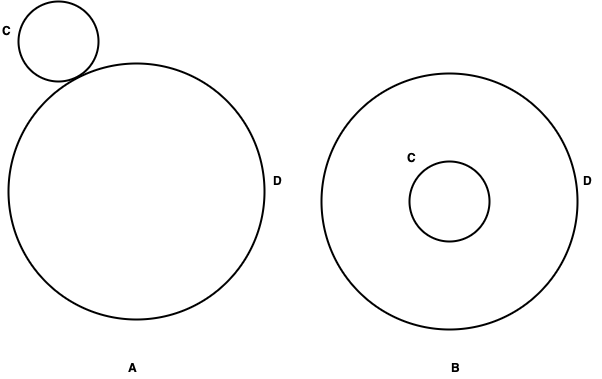
\includegraphics[scale=0.4]{graphics/center_periphery.png}
	\caption{A = the relationship between the object of cognition and the circle of the soul that Aristotle attributes to Timaeus, B = the relationship between the object of cognition and the circle of the soul as Timaeus in fact conceives of it, C = the object of cognition, D = the circle of the soul}
	\label{fig:center_periphery}
\end{figure}

Another difficulty concerns the mechanical explanation of the motion of the World Soul. The mechanical explanation requires the corporeal object to be solid and offer resistance, and the incorporeal soul to itself be solid in order to be moved by contact with the corporeal object (\citealt[129--33]{Betegh:2019fq}). The potential problem is that solidity, on some understanding of that notion, is a condition on the possibility of touch (see chapter~\ref{sec:the_elemental_composition_of_the_corporeal}). If the solidity of the extended if incorporeal soul is suitably understood, then while the World Soul may be invisible, it is tangible. When Timaeus claims that the World Soul is invisible (36e), does he allow for this? Is it really plausible that the World Soul may be felt if unseen? Or is invisible (\emph{aoratos}) an exemplar for insensible, in which case the World Soul is intangible? That Timaeus takes visibility and tangibility to be opposed extremes of the sensible provides some support for the more general reading (Proclus, \emph{In Timaeum} 2 6--7, \citealt{Diehl:1903re}, see also Calcidius' translation of 31c as well as his \emph{In Timaeum} 21, discussed in chapter~\ref{sec:the_elemental_composition_of_the_corporeal}). If the World Soul is insensible, it is intangible, and so not solid in the way required by the mechanical explanation of cognition. 

\citet[140--2]{Johansen:2004dx} is sensitive to the problem and is led thereby to deny that the World Soul has depth and solidity. Johansen observes that the sensible is the mark of the corporeal and that soul is insensible. Since the World Soul is insensible, it is intangible. And since it is intangible, the World Soul lacks the features that would make it tangible. Consider now not static touch, passively resting one's hand on an independently supported corporeal surface, but reaching out and grasping a body. What would a body have to be like to be tangible in this way. It would have to have depth and solidity. Anything that lacks depth would elude our grasp, and in grasping something with depth, it offers resistance to our grasp. And by experiencing this resistance we can have a sense of the overall shape and volume of the body in our grasp. Marking the sensible--insensible contrast thus involves making different spatial attributions to bodies and souls. Only bodies have depth and solidity as required for their tangibility in a way that our souls do not.

Part of the charm of the corporeal understanding \emph{ephaptētai} in the special case where the World Soul applies itself to a divisible being is that it provides the resources for a mechanical explanation of the World Soul's opinion about the sensible. In applying itself to divisible being, the World Soul is in corporeal contact with its object and this causes it to engage in axial rotation. The mechanical explanation exploits the spatial character of the World Soul. The World Soul does occupy the space of the Cosmos---it is stretched throughout that space. But perhaps it does not occupy space in the same way as the body of the Cosmos. Something like the following thought might have motivated Johansen: If the World Soul had depth and solidity, it would exclude the body of the Cosmos from occupying the same space. However, if the World Soul lacks depth and solidity, it may spatially overlap the body of the Cosmos. Johansen is right to insist that whereas the corporeal is tangible, the World Soul is intangible. What Johansen failed to see was that the World Soul must meet the requirements on tangibility if the mechanical explanation of the soul's movement succeeds on its own terms. In order to move the soul, the divisible being must resist the soul's application to it. But such resistance is only possible if the World Soul is itself solid. It is difficult to understand how the mechanical explanation of the World Soul's opining could be consistent the sensible being the mark of the corporeal, the conditions on tangibility, and the World Soul being insensible.

There are other difficulties with the mechanical explanation. Following \citet{Corcilius:2018bd} and \citet{Betegh:2019fq} we have retained an active sense for \emph{ephaptētai}. The present interpretation may have the World Soul in corporeal contact with divisible being, but only by the World Soul seeking out such contact. Still, the World Soul's applying itself to the divisible being merely makes it a passive recipient of imparted motion. Even if the World Soul only has the power to receive such motion if it actively applies itself to the sensible and the corporeal, there are elements of the passage that suggests that the World Soul is the initiator of that movement and not merely its recipient. On the present interpretation, the opinion, the soul's announcement concerning the divisible being that it applies itself to, is the World Soul's motion throughout its whole being that results from that contact. But later, Timaeus will speak of the announcement as being born through the self-moved. This suggests that the World Soul, in applying itself to a divisible being, moves itself and is not itself moved in reaction to the encounter. If the World Soul moves itself and is not moved by its encounter with a divisible being, then it is not a passive recipient of motion in the way that it would have to be if it were subject to the envisaged mechanical explanation. 

Even if the interpretation of \emph{ephaptētai} as involving some form of corporeal contact were to succeed perfectly on its own terms, its ambitions are limited, and this, in the end, is its ruin. It only considers a special case, the World Soul's applying itself to a divisible being. The World Soul also applies itself to indivisible beings, intelligible beings such as the Forms. There is no question of conceiving the World Soul's applying itself to the Forms as corporeal contact. Indivisible beings are not only incorporeal but inextended as well. And since only extended things may be solid, indivisible beings are not solid and so offer no resistance in corporeal contact. Either contact means different things when the World Soul is said to be in contact with divisible beings and when it is said to be in contact with indivisible beings, or contact means something sufficiently general to cover both cases. Put another way, does \emph{ephaptētai} admit of homonymous or non-homonymous reading? Insisting that \emph{ephaptētai} be read as corporeal contact when applied to divisible beings commits one to a homonymous reading of \emph{ephaptētai}. Unfortunately, the homonymous reading does not cohere with the text.

Consider, then, a homonymous reading of \emph{ephaptētai}. When applied to divisible being it denotes a kind of corporeal contact. When applied to indivisible being it denotes a kind of non-corporeal contact. One problem with the homonymous interpretations of \emph{ephaptētai} is the grammatical context of its occurrence. It occurs in a context where we are being asked to consider the World Soul applying itself to either a divisible or indivisible being. The homonymous reading should rule out such constructions. Either reading of \emph{ephaptētai}, as involving corporeal contact or not, would rule out the intelligible occurrence of one of its objects  (compare the standard linguistic tests for lexical ambiguity, \citealt{Zwicky:1975hl}). If \emph{ephaptētai} is interpreted as involving corporeal contact, while taking a divisible being as its objects is intelligible, taking an indivisible being as its object is not. And if \emph{ephaptētai} is interpreted as involving non-corporeal contact, while taking an indivisible being as its object is intelligible, taking a divisible being as its object is not. Such a construction could only be intelligible on a non-homonymous reading of \emph{ephaptētai}. The verb must mean something sufficiently general to intelligibly apply to both divisible and indivisible beings.

The homonymous reading of \emph{ephaptētai} is, if not incoherent, then inconsistent with the text. As a consequence, one should not understand the World Soul's applying itself to divisible being as corporeal contact. Whatever the occurrence of the verb means, it must mean something sufficiently general to apply to sensible and intelligible objects, and it does not on the corporeal interpretation. 

Of its range of uses perhaps only its cognitive uses are sufficiently general on a literal interpretation of them (for example, Plato, \emph{Symposium} 212a; though such cognitive uses, literally understood, are surely dead metaphors; on grasping and cognitive apprehension see \citealt{Rosen:1961aa}). One obstacle to this suggestion is that the most straightforward understanding of it is false. So consider those uses where \emph{ephaptētai} means something like cognitive apprehension. The activity conveyed by \emph{ephaptētai} may be a part of the apprehension of a sensible object in opinion but it is not the whole of it. Opining involves not only the World Soul applying itself to a sensible object, but moving itself throughout the whole of its being in response. So if \emph{ephaptētai} receives a cognitive reading, it must be less than the whole cognitive act effected. 

Perhaps \emph{ephaptētai} admits of a restricted cognitive reading. Perhaps \emph{ephaptētai} can be understood as analogous to attentive contact, an attentive contact involved in, if distinct, from the cognitive act. I stress the analogy here. \emph{Ephaptētai} is not attentive contact it is merely like it. A conception of attention as an independent cognitive activity, though Platonic in its sources, is plausibly post-Timaean. Such a conception only fully emerges in the work of Plotinus and Augustine. The analogy only attributes to Timaeus an anticipatory trace of this post-Timaean idea. Attending to a sensible object is not to opine about it. Nevertheless, in attending to a sensible object, the World Soul moves itself throughout its whole being thus announcing the character of the sensible object attended to. Similar remarks apply to the intelligible case. Attending to intelligible objects is not yet to know them. Perhaps they must be brought into relation with other intelligible objects over the course of dialectic before they are truly known. And yet one only comes to know the intelligible by attending to it. In attending to an intelligible object, the World Soul moves itself throughout its whole being thus announcing the character of the intelligible object attended to. So perhaps only a restricted cognitive reading of \emph{ephaptētai} is sufficiently general to cover the World Soul's application to divisible and indivisible being. So interpreted, \emph{ephaptētai} is a kind of pre-cognitive attentive contact at work whenever the World Soul cognizes.

There is a problem, however. While pre-cognitive attentive contact is less than the full cognitive act as required, it still does more than it should. On the present interpretation, attending to divisible or indivisible being fixes the object of the cognitive act. But plausibly the object of the cognitive act is only fully determined by the World Soul moving itself throughout the whole of its being (a problem shared with Aristotle's corporeal reading of \emph{ephaptētai}, \emph{De anima} 1 3 407a18--9, \citealt[84, 98--9 n26]{Lee:1976xs}). Consistent with a restricted cognitive reading, \emph{ephaptētai} is better understood as a kind of pre-cognitive orientation toward the object of the cognitive act. It is analogous to reaching in the act of grasping. (\citealt[276]{Ross:1906fk}, and \citealt[404 n335]{Cherniss:1944aa}, take Aristotle's description of ``reaching out'' in thought in \emph{De memoria} 2 452b9--11 to be a reference to the present passage. \citealt[98--9 n26]{Lee:1976xs}, \citealt[87]{Corcilius:2018bd} \citealt[134]{Betegh:2019fq} offer similar interpretations.) In reaching for something one does not grasp it. A body is the object of one's grasp only when one conforms one's hands to its contours and so binds it in one's grasp. Nevertheless, in reaching for a body one is orienting one's own body towards it in such a way that one may come to grasp it. It is part of the process of coming to grasp the body and not itself the grasping of it. Such a pre-cognitive orientation is less than the full cognitive act as required. And while it may help determine the object of the cognitive act, it does so consistent with that object only being fully determined by the World Soul moving itself throughout the whole of its being. The idea is that \emph{ephaptētai} is the process by which the object of cognition is identified and not its identification. Following Proclus (\emph{In Timaeum} 2 300 10--14, \citealt{Diehl:1903re}), I shall henceforth speak of this pre-cognitive orientation as the World Soul applying itself to the object of its cognition. 

In the \emph{eikōs muthos}, circular motion is a corporeal image of incorporeal cognitive activity. In light of this, the World Soul's applying itself to the object of its cognition can be pictured as follows. The World Soul's applying itself to the object of cognition is the process by which the object of cognition is identified. The object of cognition is only identified when the World Soul moves itself throughout the whole of its being. Since circular motion is the corporeal image of the latter, we can imagine the process of identification as a rounding about, a circling in on, a vortex of activity narrowing in on the object of cognition. The object of cognition is identified only when encircled by the motion to the exclusion of anything else. Thought's encirclement of its object may be active, but its object is at rest in its center. The object of the cognitive act resides in the eye of the cognitive storm.


% section _emph_ephatetai (end)



\section{Cognitive Activity} % (fold)
\label{sec:cognition}

Timaeus conceives of cognitive activity, the exercise of the World Soul's cognitive powers, as an internal discourse. In cognizing, the truth about the objects of cognition are announced. Timaeus initially provides a general description of cognitive activity. His general description applies to understanding (\emph{nous}) and knowledge (\emph{epistēme}) as well as opinion (\emph{doxa}) and conviction (\emph{pistis}). Only subsequently does Timaeus discuss how knowledge differs from opinion (we shall take up this difference in section~\ref{sec:knowledge_and_opinion}). In Peripatetic terms, Timaeus first describes the genus of cognitive activity before describing its species.

The World Soul applies itself to divisible or indivisible beings. On a restricted cognitive reading of \emph{ephaptētai}, this is a kind of pre-cognitive orientation toward the object of cognition. In applying itself to the divisible or indivisible beings, the World Soul moves throughout the whole of its being and announces the character of the object applied to. The announcement, without speech or sound, is the cognitive act, the exercise of the Word-Soul's cognitive powers. A question immediately arises. Is the movement throughout the whole of its being the same as the announcement? Or is the movement merely a phase in the causal process eventuating in cognition? Porphyry attributes the latter interpretation to Amelius who held that the announcement was made only once the World Soul ceased to move (\emph{In Timaeum} 74, \citealt{Sodano:1964mf} = Proclus, \emph{In Timaeum} 2 300 34--301 2, \citealt{Diehl:1903re}). According to Porphyry, Amelius' interpretation rested on a textual mistake. Even so, Amelius may yet be right. Thus Proclus reports that Sosicrates shared the same interpretation. So our question remains: Does the movement constitute the announcement or merely cause it?

Identifying the movement with the announcement is in one way parsimonious. Timaeus does not then have to provide a further account of what this announcement is. Though some explanation is owed as to how and in what sense this motion is an announcement. Indeed, this puts an important constraint on any such identification. The movement must be understood in such a way that it is intelligibly an announcement. If the movement could not be understood in this way, then that would be good reason to regard the movement as merely a phase in the causal process eventuating in cognition, in which case Amelius would be vindicated. The identity or difference of movement and announcement is only settled once we have a better understanding of the potential cognitive significance of the World Soul moving itself throughout the whole of its being.

Let us begin with the movement of the World Soul. The movement of the World Soul is active. The World Soul moves itself and is not itself moved in response to its application to its object. The World Soul is a self-mover (\emph{kinoumenō huph autou}) and so is not moved by coming into contact with its object. It is not the passive recipient of motion but the initiator of the motion. Application to the object is not the cause of the World Soul's movement but only the occasion for it. The movement is the activity of the World Soul. It rouses itself to this activity in applying itself to divisible or indivisible beings. The movement is less a mechanical effect than the arousal of a living being in response to contact. (Later Platonists highlight this imagery. Thus, Priscian, \emph{Metaphrasis in Theophrastum}, and Pseudo-Simplicius, \emph{In De anima}, portray the activity of the soul in perception as a mode of arousal.)

That the movement is not passively received but initiated by the World Soul itself makes it akin to cognition in at least one respect. Thinking is not something done to a thinker, but something a thinker does. The movement throughout the whole of its being is like thinking in not being passively received but actively performed by the World Soul. In Kantian parlance, it shares in the spontaneity of judgment.

There is some evidence that the movement throughout the whole being of the World Soul is not only active but discursively structured. If the movement is discursively structured, it may intelligibly be an announcement, in which case movement and announcement may be identified. Timaeus comes close to explicitly claiming as much when he tells us that the announcement is born through the self-moved without speech or sound (37b5--7). It is at least natural to suppose that the announcement is born through the self-moved by the World Soul moving itself throughout its whole being constituting the announcement. The World Soul is not merely the audience of the announcement but its author. Thinking, here, is being envisaged as the soul's conversation with itself. This is, of course, a familiar Platonic theme. (Compare \emph{Theaetetus} 190a and \emph{Sophistes} 263e, 264a--b.) Even if the announcement being born through the self-moved provides some evidence that the self-initiated movement is discursively structured, it does not yet explain how it might be.

To get a better sense of how the active motion may be discursively structured, we shall consider the account of discursive structure offered in the \emph{Sophistes} (260a--263e). Doing so shall highlight aspects of the present passage whose significance might otherwise go unnoticed. Importantly, I shall not insist on doctrinal uniformity between the \emph{Timaeus} and the \emph{Sophistes}. There are differences. The \emph{Timaeus} makes no mention of Motion and Rest as being among the greatest kinds as in the \emph{Sophistes}, and Timaeus seems to revert to explaining motion in terms of Difference (52e, 57c, 57e, 58d--e, 62b1--2). Moreover, there are real differences in emphasis. In the \emph{Sophistes}, the Eleatic Stranger is concerned to establish the possibility of false statements, whereas Timaeus is describing the true opinion and knowledge of the World Soul. The possibility of error is something only the younger siblings of the World Soul, the souls of mortal beings, must grapple with. (On the Eleatic Stranger on discursive structure see \citealt[]{Frede:1992ec}, on its relation to the \emph{Timaeus} see \citealt[]{Betegh:2019fq}.)

According to the Eleatic Stranger, making a statement requires two things. The speaker must first identify the subject of the statement, what they want to make a statement about, but they must also second specify what is said about the subject. Thus a statement must at least contain two parts, a part identifying the subject of the statement and a part specifying what that statement says of the subject. The former is a noun and the latter is a verb. To make a statement, a speaker must ``weave'' together the noun and the verb (262d4). Philoponus' take on interweaving might be appropriate here as well (\emph{In De anima} 120.35– 121.9, discussed in chapter~\ref{sec:the_embodiment_of_the_world_soul}). The interweaving of noun and verb in making a statement is neither their fusion nor mere juxtaposition. The interweaving of noun and verb is not a fusion since statements admit of decomposition into nouns and verbs and so are intelligibly differentiated. And the interweaving is not merely juxtaposition since not all juxtapositions of words make meaningful statements (\emph{Sophistes} 263d). The interweaving of noun and verb is such that what is specified by the latter is related to what is identified by the former. There are two kinds of statements, affirmative and negative statements. Affirmative statements say that things are the same and negative statements say that things are different. If what the noun applies to is different from what is specified by the verb, then different things are said as the same and the affirmative statement is false (\emph{Sophistes} 263d). Conversely, if what the noun applies to is the same as what is specified by the verb, then things that are the same are said as the same, and the affirmative statement is true. Finally, reasoning is understood as the soul's conversation with itself and opinion (\emph{doxa}) is the result of this conversation (\emph{Sophistes} 264a--b). Cognition, conceived as a kind of inner speech, must similarly display this discursive structure.

The Eleatic Stranger's discussion of the soul's conversation with itself (\emph{Sophist} 264a--b) introduces a potential complexity. There the soul's conversation with itself is understood as reasoning, the rational process by which judgment is fixed, and its result is cognition. Applying this idea to Timaeus' speech might suggest that the World Soul moving itself throughout its whole being is the process by which cognition is fixed and the announcement the result. This would be to revive Amelius' interpretation. If, however, the announcement being born through the self-moved is explained by the announcement just being the self-initiated movement, then Amelius' interpretation should be rejected, and the Eleatic Stranger's account not applied in this manner to Timaeus' speech. If anything, it is (\emph{ephaptētai}) that describes a phase in the process of fixing cognition.

The World Soul applies itself to (\emph{ephaptētai}) divisible and indivisible beings. On a restricted cognitive reading this is a pre-cognitive orientation toward the object of cognition. The identification of the object of cognition is only complete with the circular motion of the World Soul. So this is best understood as the process of coming to identify what the cognitive act is about. Timaeus' use of \emph{peri} is a deliberate pun, just as something may revolve about (\emph{peri}) its center, a thought is about (\emph{peri}) its object. The object of cognition is the subject of inner speech. It is what the announcement is about. The announcement says something about its subject, the object of cognition. If the subject of the announcement is the same as what the announcement says of it, then the announcement is true. The World Soul only makes true announcements, and the two kinds of announcements that it makes corresponds to the two kinds of statements that may be made in speech. True statements are either affirmative or negative, they either say that the same are the same or that the different are different. And this is what the World Soul's announcements do, they say that the same are the same and that the different are different (37).

Those commentators that see Timaeus, here, as subscribing to the principle that like is know by like make a connection between the cognitive activities of saying that the same is the same and that the different is different with the World Soul being composed of a mixture of Being, Sameness, and Difference. Since it is composed, in part, of Sameness, the World Soul is capable of judging the same as the same. And since it is composed, in part, of Difference, the World Soul is capable of judging the different as different. How must we conceive of this cognitive activity in order for this to be so? One way, perhaps not the only way, would be if the cognitive activity is the World Soul moving itself throughout its whole being, a being composed of Sameness and Difference.

It is tempting to envision the movement by which the World Soul announces the same as the same as the revolution of the Circle of the Same, and the movement by which the World Soul announces the different as different as the revolution of the Circle of the Different. The temptation should be resisted. First, notice that Timaeus will subsequently distinguish knowledge and opinion in terms of these. Thus when the World Soul applies itself to an indivisible being, something intelligible and incorporeal, the Circle of the Same revolves, and the World Soul understands and knows its object. And when the World Soul applies itself to a divisible being, something sensible and corporeal, the Circle of the Different revolves, and the World Soul has true opinion and conviction about its object. Second, notice that the Circles of the Same and the Different are so called not because of any substantial difference between them. Each are composed of the same mixture Being, Sameness, and Difference and with the same proportional divisions. That means that the different revolutions of the circles in knowledge and opinion could not be explained in terms of a substantial difference since they share the same substance. The principle that like is known by like has no grip here. Moreover, indivisible beings are themselves the same or different from other indivisible beings. So it would be a mistake to think that knowledge only judges the same as the same, it judges the different as different as well. And it is thanks to the Circle of the Same being composed, in part, by Difference that it may announce the different as different even among the indivisible. Similarly, it is thanks to the Circle of the Different being composed, in part, of Sameness that it may announce the same as the same even among the divisible. Both knowledge and opinion involve judging the same as the same and the different as different. Even the degraded form of cognition available to embodied mortal beings embedded in an environment, perception, involves not only discrimination but perceptual grouping as well, as when one succeeds in seeing the numeral in an Ishihara color test (see figure~\ref{fig:ishihara}).

\begin{figure}[htbp]
	\centering
		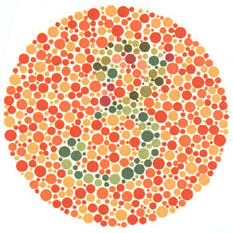
\includegraphics[scale=1.5]{graphics/ishihara.jpg}
	\caption{Ishihara Color Test}
	\label{fig:ishihara}
\end{figure}

The assumption that the movement is simple motivates, in part, the temptation to identify judgements of Sameness with the revolutions of the Circle of the Same. We should not assume that the movement that constitutes the announcement is simple. The Demiurge has fabricated a complex structure for the World Soul. He does so to invest the World Soul with the power of complex motion. The greatness of this power is visibly manifest in the complexity of celestial motion. Notice that the proportional divisions in the substance of the World Soul are not exhaustively used in Timaeus' astronomy. Given the association of the Demiurge and \emph{nous} we can be sure that the the astronomically unused proportions are not there for no reason. Moreover, suppose we follow Aristotle in holding that the soul is the principle of motion and cognition (\emph{De anima} 1 406b28--31). Then it would be plausible that the astronomically unused proportions are cognitively significant. Perhaps the complex motion associated with cognition is sufficiently complex to be discursively structured.


 

% If we abandon that assumption, new interpretative possibilities open up.

% To appreciate this, indulge me in the following speculation. The speculation is offered less as a potential interpretation than as a proof of possibility---a proof that, given the psychogony as Timaeus presents it, the motions of the World Soul are sufficiently complex to be discursively structured by the lights of the \emph{Sophist} account.

% Consider the World Soul applying itself to a divisible being and announcing its character in true opinion. Suppose the World Soul applies itself to Theaetetus and so comes to cognize this divisible being. To cognize Theaeteus is to engage in circular motion. Since it is Theaetetus that is cognized, presumably he is at the center of this circular activity. That is what it means for a divisible being to be the object of cognition. In cognizing Theaetetus, the World Soul recognizes his activity as sitting. To recognize Theaetetus' activity is itself to engage in circular motion. However, since the World Soul is complex, we need not assume that it is the same circular motion as the one that cognizes Theaetetus. Not only has the Demiurge invested the World Soul with a complex structure, He also imposed proportional divisions within its substance. And this opens up the possibility of understanding interweaving within Timaeus's \emph{eikos muthos}. In this case, the proportional divisions of the World Soul are the warp its two revolutions are the weft. Perhaps the two motions are interwoven in the sense that they are harmonious or attuned to the proportional divisions providentially established in the substance of the World Soul. As on Philoponus' take on interweaving, the two circular motions are neither fused nor juxtaposed. They are not fused. The circular motions remain two and the movement constituting the announcement is complex. Nor need they be juxtaposed. Indeed what could juxtaposition even here mean? Interweaving is rather the harmony of their revolutions. On this interpretation, judging the same as the same is the complex motion involving two revolutions attuned to one another. The World Soul's opinion consists in its moving itself throughout its whole being in this complex harmonious fashion. Undoubtedly, the motion is even more complex. The World Soul not only judges thing the same or different, but in what respect, in what manner, when, and where. These must be constituted by either component motions of the complex motion, their properties (such as rate of revolution), or the component motions being appropriately related (such as being attuned in some way).

% The interpretation is not only speculative but incomplete insofar as no specific part of the complex structure has been identified as moving. Nor is it clear how negative statements of inner speech are meant to work. If the components of the complex motion of affirmative statements are concordant, are we to imagine that the components of the complex motion of negative statements are discordant? It is clear that on the model given above this needs to be represented in terms of the proportional divisions within the substance of the World Soul, but how exactly? Despite these limitations, the interpretation illustrates how the Timaean position may be developed once we give up the assumption that the movement is simple. Allowing for the complexity of the World Soul's movement at the very least makes it possible for it be discursively structured.

% section cognition (end)

\section{Knowledge and Opinion} % (fold)
\label{sec:knowledge_and_opinion}

So far, we have been discussing the cognitive activity of the World Soul generally. There are two species of cognitive activity that the World Soul engages in corresponding to its two kinds of objects. The World Soul either applies itself to divisible or indivisible beings. Opinion (\emph{doxa}) and conviction (\emph{pistis}) take divisible beings as their objects, whereas understanding (\emph{nous}) and knowledge (\emph{epistēme}) take indivisible beings as their objects. 

The two species of cognitive activity are not merely distinguished by their objects. It is not just the objects of cognition that distinguish knowledge from opinion, but the character of these acts differ as well. Moreover, the character of the acts differs in three ways. First, opinion and knowledge differ in that they involve the World Soul moving different parts of itself. Second, opinion and knowledge differ in that the movements themselves differ. Third, the resulting cognitive states, opinion and knowledge, are differently described, as true proclamation and disclosure. More explicitly:
\begin{enumerate}[(1)]
	\item Whenever the World Soul takes something sensible from the realm of Becoming as the object of its cognition:
	\begin{enumerate}
		\item the Circle of the Different moves
		\item in a straight course (\emph{orthos})
		\item and proclaims it to the whole soul
	\end{enumerate}
and this is true opinion and conviction.
	\item Whenever the World Soul takes something intelligible as the object of its cognition:
	\begin{enumerate}
		\item the Circle of the Same moves
		\item by spinning truly (\emph{eutroxos})
		\item and thus discloses its object
	\end{enumerate}
and this is understanding and knowledge.
\end{enumerate}

(a) Opinion involves the revolution of the Circle of the Different while knowledge involves the revolution of the Circle of the Same. This is not a reflection of any substantial difference between them. Both are composed of the same mixture of Being, Sameness, and Difference, with the same proportional divisions. Moreover, the World Soul needs to judge the same as the same and the different as different with respect to both the sensible and the intelligible. That the circles are composed of Sameness and Difference allows them to do just that by the principle that like is known by like. If the motion of the different parts is not explained by a substantial difference between them, then why is \emph{doxa} and \emph{pistis} associated with the movement of the Circle of the Different and \emph{nous} and \emph{epistēme} with the the movement of the Circle of the Same?

That the Circle of the Same comprehends the intelligible is a manifestation of the sovereignty granted to it by the Demiurge. It was this sovereignty that allowed the Circle of the Same to remain undivided unlike the Circle of the Different. Perhaps the integrity and order of the seven circles of the Different are sustained by the power and authority of the Circle of the Same whose wisdom derives from contemplating the intelligible. The Circle of the Different is not sovereign but is governed. That it comprehends only the sensible and the corporeal is a manifestation of its inferior status. At least in mortal beings, opinion is connected with \emph{aisthēsis} and the linear motion of \emph{aisthēsis} is the source of turbulence and ethical unrest. It is well that such is governed by the wisdom that contemplating the intelligible brings. The World Soul is not troubled by embodiment the way that the souls of mortal beings are, in part, because it is not embedded in an environment with strong powers. Nevertheless, as elder sister, World Soul exemplifies the cognitive psychology that virtuous mortals must display if they are to face well the ethical challenges of this corporeal life. The motion of the different parts of the World Soul is not explained by a substantial difference between them. There is no substantial difference between the Circles of the Same and the Different. Rather, different parts of the World Soul are moved in knowledge and opinion because the one rules and the other is ruled, an arrangement that is rational, harmonious, and providentially significant.

(b) Opinion and knowledge differ not only in that the World Soul moves different parts of itself, but the movements of the different parts themselves differ. Whereas the Circle of the Different moves in a straight course (\emph{orthos}), the Circle of the Same spins truly (\emph{eutroxos}). This might seem puzzling at first. After all, both are circles, and so both revolve. So in what sense is the course of the Circle of the Different straight? Consider, then, three hypotheses. It is unclear which, if any, apply.

First, motion, for Timaeus, is either circular or linear and there are six forms of linear motion. The oppositional structure here is one--many. Perhaps a complex motion may be more or less circular or more or less linear depending upon the motions from which it is compounded. On the first hypothesis, the Circle of the Different, though it revolves, its motion is complex and involves its circular motion compounding with linear motion. The Circle of the Same, by contrast, is either purely circular or is compounded with significantly less linear motion. This at least seems apt with respect to the mortal counterparts of the World Soul. It might seem natural that the motion of the Circle of the Different, though circular, be compounded with linear motion given the impact of linear \emph{aisthēsis} (the dramatic effects of which are vividly described in the shock of embodiment).

Second, perhaps the straight course of the Circle of the Different is not a matter of being compounded with linear motion so much as an appearance induced by the partial perspective from which its revolution is described. Think of a salient point on one of the circles of the Different. In the visible realm, a wanderer in its orbit would do. The wanderer moves along the path of the revolution of one of the circles of the Different. But from its perspective, it does not revolve so much as it suffers forward motion.  Taken as a whole the circle revolves, in so revolving a part of the circle suffers forward motion. On the second hypothesis, it is a perspective relative aspect of the revolution that is described as straight, rather than a component motion. What is the cognitive significance of this? Perhaps \emph{nous} and \emph{epistēme} are more of a whole than \emph{doxa}, the indivisible Being of their objects making it possible to be more intimately united with them than with the divisible Being of the sensible and the corporeal. Moreover, the Circle of the Different is itself divided into parts. Perhaps the partial perspective from which its activity is described is also a reflection of this as well as the divisible character of its object.

The first two hypotheses share the assumption that moving in a straight course is a distinctive feature of the motion of the Circle of the Different. Perhaps, Timaeus is describing the motion of the Circle of the Different in terms of a general feature that it shares with the motion of the Circle of the Same. Perhaps, Timaeus has in mind what he elsewhere describes as \emph{pros ta auta}, that the motion is always in the same direction. If Timaeus is describing a general feature common to the motions of the Circles of the Same and the Different, then, on this hypothesis at least, he has failed to specify a motion that differentiates \emph{doxa} from \emph{nous}. Perhaps, while the motion of the Circle of the Different does not have a feature that distinguishes it from the motion of the Circle of the Same, the motion of the Circle of the Same has a feature that distinguishes it from the motion of the Circle of the Different. Even if they are not differentiated by their motion, \emph{doxa} and \emph{nous} would remain different species of cognitive activity since they involve the motion of different parts of the World Soul in their apprehension of their different kinds of objects.

If, however, we retain the idea that different species of cognitive activity are associated, not only with different moving parts, but with different motions, then, however we are to understand the contrast, that the motion of the Circle of the Same is somehow more purely circular is appropriate given its sovereignty over the Circle of the Different.

(c) When the World Soul applies itself to a divisible being, it moves the Circle of the Different within. It is the World Soul that in this way opines, and not the Circle of the Different. This is why Timaeus describes the movement of the Circle of the Different as proclaiming the the sensible object to the whole soul. The World Soul is not merely a passive recipient of this proclamation. The whole soul receives the proclamation without speech or sound. But the whole soul does not merely listen, in its way, to the silent proclamation of a part, but it is the whole soul that proclaims and so opines by moving that part. (Compare: It is I, and not my arm, that hails the bus by my arm's movement. It is I, and not my arm, that Thatcher intended to shame for taking a bus beyond the age of 26.) When the Circle of the Different moves, it is the the World Soul that moves a part of itself and so proclaims truly about the sensible and the corporeal. 

When it comes to understanding and knowledge, however, Timaeus shifts the cognitive metaphor. Understanding and knowledge are not so much as proclaimed as revealed. Understanding and knowledge disclose the character of their intelligible objects. What is at stake here is not how the movement of a part may be the activity of the whole so much as the cognitive significance of such movement. The revolution of the Circle of the Same discloses its intelligible object. Timaeus' language, here, is sufficiently striking and dramatic, the Circle of the Same disclosing the intelligible, that proclaiming truly about the sensible seems impoverished by contrast. If opinion is a report, knowledge is an encounter. The former may report the truth, but in the latter the truth is unveiled. Compare the contrast between testimony and first-hand experience. 

A puzzle about the nature of the opinion arises at this point in Timaeus' speech. Opinion is connected with perception. Given that the World Soul has the cognitive power to frame true opinion about the sensible and the corporeal, does that mean that it has the power of perception as well? This can seem unlikely, since the Cosmos has been deprived of the instruments of perception. The Cosmos lacks an environment, and so has no need of the instruments of environmental powers, powers that are only ever exercised in an environment. But perception, or at least the familiar mortal kind, is an environmental power, taking as its object aspects of the environment. This would suggest that the Cosmos lacks perception. But if there is no cosmic perception, then given the connection between \emph{doxa} and \emph{aisthēsis}, how can the World Soul so much as opine about the sensible and the corporeal? It would seem that Timeaus must either:
\begin{enumerate}[(1)]
	\item deny that \emph{doxa} depends upon \emph{aisthēsis} generally, while mortal opinion depends upon perception, cosmic opinion does not, or
	\item deny that \emph{aisthēsis} is an environmental power generally, while mortal perception is environmental, cosmic perception is not. 
\end{enumerate}

Let us briefly consider both alternatives.

First, Timaeus might deny that the Cosmos has perception and maintain that while mortal opinion depends upon perception, cosmic opinion does not. How does mortal opinion depend upon perception? One way that mortal perception contributes to opinion is by identifying the subject of inner speech. One perceives Theaetetus, recognizes that he is sitting, and opines that Theaetetus is sitting, this being proclaimed throughout one's whole soul by the complex and harmonious movement of the Circle of the Different. Theaetetus is the subject of this proclamation and was identified by perception. If the Cosmos lacks perception, how, then, are the subjects of true proclamations identified? One suggestion might be that the subjects of true proclamations are what the World Soul applies itself to. 

This may depend not only upon a cognitive reading of \emph{ephaptētai}, but a particular cognitive reading. Perception is a mode of sensory apprehension. If \emph{ephaptētai} parallels perception in the fixation of Cosmic opinion, then it to must be a mode of apprehension. But it cannot be read as cognitive apprehension (as its occurrence at \emph{Symposium} 212a must be) since \emph{ephaptētai} is less than the whole cognitive act. In response to this difficulty we considered two restricted cognitive readings (section~\ref{sec:_emph_ephatetai}):
\begin{enumerate}[(1)]
	\item \emph{ephaptētai} is a kind of pre-cognitive attentive contact with the object of cognition
	\item \emph{ephaptētai} is kind of reaching out toward the object of cognition, a pre-cognitive orientation toward that object
\end{enumerate}
The first restricted cognitive reading can seem to provide an attractive resolution. The Cosmos lacks perception and so cannot identify by means of perception the subject of its inner speech. But attention, like perception, is a mode of apprehension. If the World Soul may selectively attend to different aspects of the sensible realm of Becoming, then it has the means of identifying the subject of inner speech without perception. The difficulty with this reading was that it is implausible to think that the object of cognition is wholly determined prior to the cognitive act. This motivated the second restricted cognitive reading of \emph{ephaptētai}. The idea is that \emph{ephaptētai} is the process by which the object of cognition is identified and not its identification. The second restricted cognitive reading of \emph{ephaptētai} thus plays a role disanalogous to the role that perception plays in the fixation of mortal opinion. But perhaps this has to do with the difference between mortal and cosmic perspectives. The objects of mortal opinion are external to mortal beings whereas the objects of cosmic opinion are internal to the Cosmos and so require no instruments to identify. 

Second, Timaeus might maintain that opinion depends upon perception quite generally and attribute perception to the Cosmos. The Cosmos lacks an environment and so lacks environmental powers and their instruments. So if the Cosmos has perception, perception must not be environmental generally. While mortal perception is environmental, cosmic perception is not. Proclus (\emph{In Timaeum} 2 83.3–85.31, \citealt{Diehl:1903re}) gives an interpretation of this kind (for a contemporary defence of this Proclean interpretation see \citealt{Reydams-Schils:1997aa}). Allow me to illustrate the second alternative by presenting the Proclean interpretation in terms that we have developed over the course of our discussion.

Proclus claims that cosmic perception differs fundamentally from mortal perception. Mortal perception is environmental. Mortal beings are embodied and embedded in an environment that circumscribes them. The power of mortal perception is only ever exercised in an environment and takes as its object aspects of that environment. Thus a distinction is marked between the perceiver and the object of perception. The Cosmos, while embodied, is not embedded in an environment. Beyond the limits of the Cosmos is neither space nor void. The Cosmos does not have an environment, it is the environment. Thus, if the Cosmos possesses the power of perception, it must not be an environmental power. As Timaeus' arguments about cosmic morphology make clear (33b8–34a8, discussed in chapter~\ref{sec:the_shape_of_the_Cosmos}), the Cosmos has a smooth and even surface since it has no need for the instruments of environmental powers that would disrupt that surface. The Cosmos is also comprehensive (discussed in chapter~\ref{sec:the_comprehensiveness_of_the_Cosmos}). It contains within itself all that is sensible. If the Cosmos perceives Theaetetus sitting, the Cosmos perceives a part of itself. Theaetetus is a fleeting part of the Cosmos, composed of material borrowed from the Cosmos and destined to return, as are all other mortal beings. Cosmic perception is thus a mode of sensory self-awareness that Proclus likens to consciousness (\emph{sunasithēsis}). Cosmic perception is akin to bodily awareness. Just as one may be aware of the configuration and activity of one's limbs without the aid of external observation, the Cosmos is aware of the configuration and activity of its parts. 

Cosmic perception differs from mortal perception. Cosmic perception has no need of instruments to operate in an environment. And no distinction is drawn between perceiver and object of perception. But cosmic perception also differs from mortal perception in a further way, in not being divided into the special senses. Timaeus distinguishes the special senses of mortal beings in terms of the parts of the body in which they receives violent affections from without in the causal process that eventuates in perception (65b–68e). But the Cosmos does not receive violent affections from without. There is nothing without to affect it. That is why it is immune to disease and ageing. Cosmic perception remains undifferentiated because, though embodied, the Cosmos is less involved with corporeality than encosmic beings, not being subject to strong powers from without. 

Cosmic perception, being a general mode of sensory self-awareness, has no need of affection from without. There is nothing sensible without the Cosmos. The Cosmos contains all that is sensible. And so it enjoys a general mode of sensory self-awareness, more unified and superior to the special senses of mortal beings. And it is upon this general mode of sensory self-awareness that cosmic opinion depends. The Proclean resolution is ingenious, but suffers from a lack of textual support, though reflection upon it reveals just how closely it adheres to claims that Timaeus in fact makes.

% section knowledge_and_opinion (end)

\section{The Cognitive Significance of Circular Motion} % (fold)
\label{sec:the_cognitive_significance_of_circular_motion}

Motion is either circular or linear. The opposition is one-many, there being six forms of linear motion. Circular motion is rational, and linear motion is irrational. If the opposition were to figure in a development of the Pythagorean table of opposites, circular motion would be in the superior column. 

But why is circular motion rational? What is the connection between cognition and revolution? While Timaeus clearly presupposes such a connection, he never makes that connection explicit. The connection between cognition and revolution is presupposed in two passages. At 34a3-4 the Demiurge assigns to the body of the Cosmos one of the seven motions associated with \emph{nous} and \emph{phronesis}, circular motion, which Timaeus describes as turning uniformly in the same place within itself. At 40a7--b1 Timaeus claims that the fixed stars revolve and goes on to connect this with their sustained thinking. One of the two motions of the fixed stars is uniform and in the same place, and the fixed stars always think the same thoughts about the same objects. Both passages presuppose that there is a connection between cognition and revolution, but neither passage explains what that connection is (\emph{pace} \citealt[119]{Cornford:1935fk}, see \citealt[72--3]{Lee:1976xs}). Perhaps, Timaeus feels free to presuppose a connection between cognition and circular motion because he is drawing upon and elaborating an Eleatic tradition of linking the two. Indeed the features of the circular motion that Timaeus finds cognitively significant for the most part have antecedents in Parmenides (on Parmenides and Timaeus on circular motion see \citealt{Ballew:1974hw}.)

If we are to understand the connection between cognition and revolution, we should begin by surveying the features that Timaeus ascribes to circular motion. Specifically, circular motion is:
\begin{enumerate}[(1)]
	\item about something (\emph{peri ta auta})
	\item that it is bound to
	\item throughout the whole
	\item uniform (\emph{kata tauta})
	\item in the same place or within its limits (\emph{en tō autō})
	\item in the same direction (\emph{pros ta auta})
\end{enumerate}
These features are not as distinct as their enumeration may suggest. A question to bear in mind as we review these is whether these are features of circular motion generally, or whether at least some of these are features of specific circular motions that Timaeus finds cognitively significant. It will emerge that Timaeus has provided a specific kind of circular motion as a corporeal image of cognitive activity.

(1) \emph{Circular motion is about something (\emph{peri ta auta})}. Circular motion is about or around something. A revolving circle moves round about itself. More specifically, it has a center or central axis around or about which it revolves. This is a general feature of circular motion. 

In the first instance I translated \emph{peri} as about to bring out the connection with the preposition's use to specify the object of cognition (see, for example, 40a7--b1). Just as the circular motion is about something, a center or central axis around which it revolves, thoughts are about their objects.

The pun can be found in Homer, where the body of dead comrade may be fought about (\emph{amphi} or \emph{peri}) both in the sense of the body being the object of the fight and in the sense that it is fought around the body. While the origin of the pun is Homeric, it seems to have enjoyed an Eleatic revival (\citealt[191--3]{Mourelatos:2008ve}). Parmenides maintains that only Being is intelligible. And so only Being is the object of thought. Parmenides conceives of Being as spatially extended and finite, in the shape of a sphere. If the thought that thinks the One Being involves spatial movement, it could only go around that sphere. Thought is about its object by going around it. Thus the unnamed goddess that reveals the Ways of Truth and Mortal Opinion to Parmenides proclaims that her thought is \emph{amphis alētheis}.

While Timaeus agrees with Parmenides that there is a mode of Being that is spatially extended---divisible Being---a crucial difference remains. Timaeus countenances, in addition, a mode of being that is not spatially extended---indivisible Being. This is a post-Parmenidean innovation. Parmenides (the historical Parmenides, not the eponymous character of the dialogue) seems never to have considered the possibility of being without extension.

Timaeus retains this Eleatic pun, despite rejecting the Parmenidean claims upon which it depends. Indivisible beings are the intelligible objects of \emph{nous}. As they are without extension, there is no spatial movement around (\emph{peri}) them, the way there is around the sphere of the One Being on Parmenides' account. Parmenides holds that all objects of thought are spatially extended. Timaeus, by contrast, holds that not all objects of thought are spatially extended and so not all thought so much as could be circular movement around an extended thing.

And yet the Eleatic pun of thought being about (\emph{peri}) its object is retained. There is a shift of sense here. For Parmenides, thought literally moved around its object. That is what made the pun apt. (``It's funny because it is true!'') For Timaeus, however, not all objects of thought are such that thought could move around them. What, then, for Timaeus, makes the Eleatic pun apt? The very fact that it is something different from what it was for Parmenides by itself establishes a shift of sense. And not just in what was meant but perhaps also in the meaning of it. While for Parmenides the spatial connotations of \emph{peri} could be taken literally, for Timaeus they are a metaphor at best, at least when it comes to \emph{nous}.

What, then, for Timaeus, makes the metaphor apt? The object of cognition is what the cognitive act is about. In imagining cognitive activity as spatial movement around its object, the cognitive act circumscribes and encompasses its object. That circular motion encompasses what it moves about describes the relationship between the cognitive act and its object. The imagery, here, persists as a dead metaphor in professional philosophical parlance. The object of cognition is the \emph{content} the cognitive act. The object is the content of the cognitive act only if the cognitive act encompasses that object so as to contain it. 

That circular motion encompasses what it moves about may describe the relationship between the cognitive act and its object, but the fact that it is movement that encompasses the object should not be overlooked. The object of cognition may be the content of the cognitive act insofar as it is encompassed and so contained. But the container is unlike a corporeal container. It is not a body, like a \emph{kratēr}, but an activity. Nor is it a corporeal activity. The sensible is the mark of the corporeal, and the World Soul is insensible. So the cognitive activities of the World Soul are incorporeal activities. The object of cognition is encompassed by the incorporeal activity about it.

(2) \emph{Circular motion is bound to the center around which it revolves.} Of the enumerated features this is perhaps the most implicit. The circular motions of the World Soul and the body of the Cosmos are centripetal. This is perhaps clearest with respect to the body of the Cosmos. The revolution of the Circle of the Same determines the revolution of the fixed stars in the Heavens and this motion extends downwards to the center of the Cosmos \citep[32]{Vlastos:1975aa}. In this way, it governs interior revolutions with different axial rotations, such as the revolutions of the wanderers in the sidereal ecliptic plane as determined by the revolution of the Circle of the Different.

There may also be a hint of it in the World Soul applying itself to its object before moving itself. The verb, \emph{ephaptētai}, can be used to convey \emph{binding}, somehow \emph{fixing} or \emph{holding fast} (Homer, \emph{Odyssey} 22 41). And the binding imagery persists in the tactile uses of the verb such as \emph{laying hands on} (Homer, \emph{Odyssey} 5 348). And in \emph{grasping}, understood as a mode of haptic perception, the perceiver binds their hands to the contours of the body grasped and thereby feels its overall shape and volume. And with respect to the cognitive uses of the verb, it is plausible to think thought is bound to its object. (This might itself be an Eleatic echo, \citealt[192]{Mourelatos:2008ve}.) If it was bound to a different object it would be a different thought. And if it was bound to nothing, it would be no thought at all. In the case of \emph{nous}, that object is only bound when the object is understood. What the verb \emph{ephaptētai} describes is the process which eventuates in the object being bound by \emph{nous}. Moreover, this process is the psychological activity of the soul. It is the soul actively seeking out its object to bind itself to. 

Moreover, binding is a means of assimilation. The soul assimilates to what it binds itself too. Soul's assimilation to the object of its cognition is for mortal beings both an ethical challenge and the means to overcome it. If one binds oneself in thought to the sensible and the corporeal, one thinks only mortal thoughts and one's soul correspondingly becomes mortal to the extent that is possible. However, if one binds oneself in thought to the intelligible and incorporeal, then one thinks only immortal thoughts and one's soul correspondingly becomes immortal to the the extent that is possible (90b--c). And when we observe the revolutions of the Heavens, with rational interest and attention, we may, over time, align the circles in our soul with the circles in the World Soul whose movement is visibly manifest in the celestial revolutions (47a--b). And in hearing, with understanding, rational speech or music, we become attuned to the proportional divisions in the World Soul (47c--e, 67a--c, 80a). The Young Gods providentially provide us with vision and audition so that we have the means to assimilate to the immortal and divine, the World Soul, our elder sister who sets a dignified example for us to emulate.

Is being bound to its center meant to be a general feature of circular motion the way that being around or about something is, or is this a feature of the specific circular motion that Timaeus finds astronomically and psychologically significant? It is not meant as a general feature of circular motion, if only because it is implausible for Timaeus to deny that circular motion may be centrifugal, especially given the use of slings in antiquity. Consider, for example, Xenophon's report, in \emph{Anabasis}, of how the Greek mercenaries sent in aid of Cyrus were regularly harassed by Persian slingers. Homer reports the use of slings, and slings were used by the Assyrians and the Persians as well as the Hebrews. Though the Hellenic Greeks favored close combat over the use of projectiles, they deployed slings as well, and the best Hellenic slingers hailed from Rhodes. 

Slings are swung in a circular fashion, and the forward linear trajectory of their ammunition crucially depends upon their centrifugal motion. In Newtonian mechanics, this assumes a frame of reference that rotates with the ammunition so that, relative to it, the ammunition is stationary. In an inertial frame of reference, by contrast, centrifugal forces need not be postulated to explain the forward trajectory of the ammunition. Release from the centripetal force of the sling and Newton's First Law of Motion would suffice. Thus the rotating frame of reference requires the postulation of centrifugal force in a way that the inertial frame of reference does not. However, the present point is not that centrifugal force is indispensable to explaining slinging a projectile. Rather, the point is that the experience of slinging a projectile is phenomenologically vivid and widely shared and so could provide one with a conception of centrifugal motion.

The ammunition varied, though lead pellets were the most effective. Many are marked with ironic or inflammatory inscriptions. The British Museum has a lead pellet inscribed with {\sbl ΔΕΞΑΙ}, ``Catch!'' (see figure~\ref{fig:dexai}). Thus centrifugal motion is common enough, in Hellenic experience, to be the object of military wit. And Critias, in detailing the forces of Atlantis, counts slingers among their troops (\emph{Critias} 119b). It is implausible, then, to think that Timaeus mistook all circular motion to be centripetal. So being bound to its center is not meant as a general feature of circular motion. Centripetal motion thus must have a special cognitive significance for Timaeus.

\begin{figure}[htbp]
	\centering
		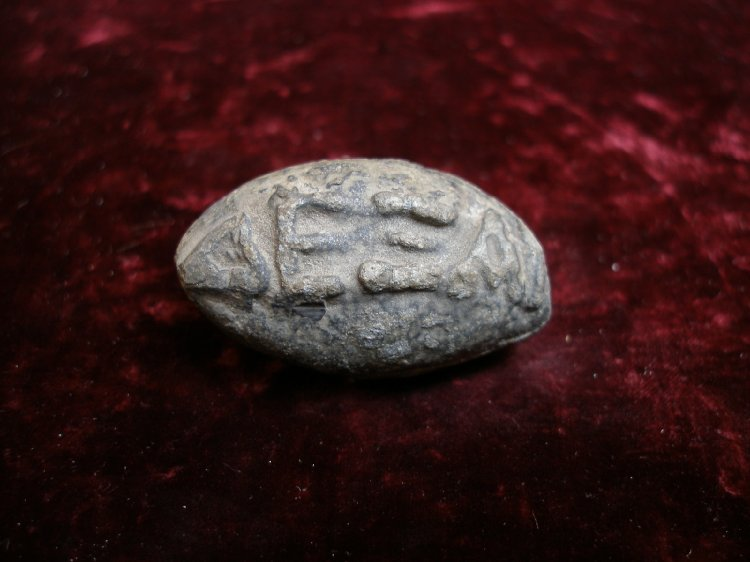
\includegraphics[scale=0.3]{graphics/dexai.jpg}
	\caption{Lead sling bullet with the inscription {\sbl ΔΕΞΑΙ}, ``Catch!'', 4th century BCE, British Museum}
	\label{fig:dexai}
\end{figure}

If being bound to its center is not a general feature of circular motion, then it is a feature of a specific motion that Timaeus finds astronomically and psychologically significant. But what is the cognitive significance of centripetal motion? What is the cognitive significance of the circular motion being bound to its center? By the Eleatic pun, what the motion is about, its center, is what the thought is about, its object. The motion is bound to its center. So, by the Eleatic pun, thought must be bound to its object. Centripetal motion provides us with a corporeal image of cognition, where the soul binds itself to the object that its activity circumscribes and so assimilates to it. Three claims may be distinguished. First binding suggests that the cognitive act and its object are united if distinct. Second, binding suggests that the soul is the agent of the union. Third, that soul binds itself to the object of cognition suggests that the identity of the cognitive act depends upon its object, that with which it unites. The soul's activity submits its identity to its object's determination. And the object determines the identity of the activity so long as that activity persists. This is the means by which the soul assimilates to the object its cognitive activity (90b--c).

While the first feature was a general feature of circular motion, the second was a feature of the specific circular motion that Timaeus finds cognitively significant. Nevertheless, both concern the intentionality of cognitive activity. The first registering the fact that cognitive activity is about something, and so describing the relationship between the cognitive act and its object, and the second describing a feature of that relationship and a consequence of it, that the soul binds itself to the object that its activity circumscribes and so assimilates to it.

(3) \emph{Circular motion is throughout the whole.} There are two separable claims in the vicinity. Both might be in play. First, it might be a claim about agency---it is the whole that moves. Second, it might be a claim about the character of the movement, that it moves as a whole. A third possibility is that Timaeus perhaps intends to combine them in some way. Let us consider these in turn. 

First, perhaps it is the whole that moves. The World Soul applies itself to an indivisible or divisible being and so announces its character throughout the whole of the self-moved. The motion which is the announcement is the self-initiated motion of the whole. When the World Soul applies itself to the object of cognition, it moves itself throughout the whole of its being. This is a claim about the agent of the motion. Even if it is a proper part of the whole that moves, be it the Circle of the Same or the Circle of the Different, in so moving the whole soul moves. In moving the proper part rebels not but its motion is proper to the whole. Cognition is personal. It is the cognizer that cognizes, even if cognizing involves the activity of special parts of the cognizer. The whole soul understands the announcement of the movement of its part because the whole soul is its author.

Second, perhaps the circular motion being throughout the whole is not meant, or at least not merely meant, to be a claim about what moves, the whole. Perhaps, it is also meant as a claim about the character of the motion, that it moves as a whole. Perhaps this is easiest to appreciate with the motion of a whole with divisible parts. So consider five satellites orbiting the Earth. Suppose that they are in the same orbit and maintain a constant rate of revolution so that their radial dimensions remain constant. Just as each individual satellite revolves around the Earth, collectively the satellites revolve around the Earth. But there are differences. An individual satellite may not have completed its period of revolution and so as of yet not revolved around the Earth and yet collectively the satellites have been revolving around the Earth all along. \citet{Lee:1976xs}, following \citet{Vendler:1967ab}, distinguishes between an accomplishment sense of revolution and an activity sense of revolution. The former is divisible into parts. Thus an individual satellite may be one quarter or one half way through its revolution around the Earth. The latter is indivisible. The satellites collectively are simply revolving. There is no sense in which they are half way through their revolutions. The former is only complete when the object circles back to its starting point. The latter is complete at every moment. So while an individual satellite may complete its revolution only once it returns to its starting point, the revolution of the satellites, considered collectively, is complete at every moment. Revolution, in the activity sense, moves as a whole.

Third, perhaps these two ideas may be combined. Suppose that it is the whole that moves. The World Soul in applying itself to the object of cognition moves itself throughout the whole of its being in a complex and harmonious fashion. The whole soul may be the agent of the activity even if it is only a part of the soul that moves, the Circle of the Same or the Different, say. However, even in the case where the whole soul moves a part of itself, that part moves as a whole. If it revolves, it does so in the activity sense of revolution. 


(3) \emph{Circular motion is uniform (\emph{kata tauta}).} Timaeus repeatedly attributes this feature to circular motion (34a3, 36c2, 40a7). Uniformity may be assessed along different dimensions, however. Moreover, uniformity may be meant in more specific and more general ways. What, then, is the intended sense of uniformity? 

If Timaeus has in mind the axial rotation of a circle or a voluminous sphere, then perhaps the main intended sense of uniformity may be its unvarying rate of revolution. Still, along these lines, there will be alternatives. Uniformity might consist, for example, in the constant curvature of the path of revolution. On any such interpretation, uniformity is not a feature of circular motion generally. A motion may have a decreasing rate of revolution or, have a path with inconstant curvature, say, and still be circular, at least by some reasonable standard.

% Uniformity understood as unvarying rate of revolution is a feature of specific circular motions that are astronomically and psychologically significant. However, we should be open to other ways in which circular motion, especially when associated with thought, may be uniform. Relatedly, we should be open to these other ways varying in their generality.

Perhaps, however, Timaeus has in mind a notion of uniformity connected with the movement of a whole. The revolution of the whole revolving itself as a whole is uniform. Since revolution in the activity sense is indivisible, each moment of its revolving is a revolving. The activity is uniformly a revolving throughout the duration of its performance. So understood, this is not a feature of circular motion generally. A motion may be a revolution in the accomplishment, as opposed to the activity sense, say, and still be circular. Should it stop short of a revolution then it would not have been a revolving. And so it is not uniformly a revolving throughout its performance.

So interpreted, uniformity is the dynamic analogue of the uniformity of Parmenides' One Being. Both are a kind of self-similarity. The uniformity of the One Being is its self-similarity throughout the extent of the voluminous sphere. The uniformity of revolution in the activity sense is its self-similarity throughout the duration of its performance.

This might be a deliberate Eleatic echo. Consider the Eleatic pun where what the motion is about, the center, is what the thought is about, its object. The One Being is the intelligible object of thought. It is spherical and so any motion that encompasses it would have to be circular. If further, the motion is revolution in the activity sense, then the uniformity or self-similarity of the One Being is mirrored by the uniformity or self-similarity of the motion that encompasses it. It is plausible that the uniformity of the motion is inherited from the uniformity of what it is about. In revolving as a whole and so in a self-similar fashion, the motion assimilates to its self-similar object. Perhaps only a self-similar motion may encompass the self-similar. Perhaps part of what it is to cognize the uniformity of the One Being is to move uniformly about it.

We have observed Timaeus' tendency to retain the Eleatic pun even while rejecting the Parmenidean claims upon which it rests. In particular, Timaeus countenances indivisible Being, a kind of Being that is not divided around bodies and so not spatially extended. As indivisible beings are without extension, there is no spatial movement around (\emph{peri}) them, the way there is around the sphere of the One Being on Parmenides’ account. According to Timaeus, however, indivisible beings are the intelligible objects of \emph{nous}. So for Timaeus, not all objects of thought are such that thought so much as could move around them. The Eleatic pun is nevertheless retained and so transformed into a cognitive metaphor. 

Perhaps this Timaean tendency is presently in play. Perhaps the Eleatic pun is retained despite rejecting the Parmenidean claims upon which it rests to highlight what is of cognitive significance. If the circular motion is centripetal, and so bound to the object which it is about, perhaps the uniformity of motion is inherited from the unity of the object that it is bound to. Perhaps, then, at least with respect to \emph{nous}, the self-similarity of the cognitive activity is inherited from the self-similarity of its intelligible object. Perhaps, at least with respect to \emph{nous}, the self-similarity of the cognitive activity, is part of what allows it to cognize the self-similarity of its intelligible object. If so, then the principle that like is known by like is not restricted to substantial likeness, such as being alike in being composed of fire. That the activity is self-similar throughout the duration of its performance is not due to the substance of the agent of the activity. It is a formal feature of the activity and a dynamic analogue of a formal feature of indivisible Being. 

The opinable are not perfectly self-similar the way the intelligible are. But perhaps this interpretation can be extended to \emph{doxa} and its objects in the following fashion. The objects of \emph{doxa} are divided around bodies and subject to change. This allows for both spatial and temporal variation in their qualities. So divided beings need not be perfectly self-similar. Suppose, however, that there is more unity to a divided being than being the content of an arbitrary region of the Receptacle. Contrast the region of the Receptacle occupied by an encosmic divided being, the body of the Moon, say, and the corresponding region of the Receptacle in the pre-cosmic chaos, before the Demiurge has imposed form and number (\emph{eidesi kai arithmois} 53b) upon it. The content of the former is a whole in the way that the content of the latter is not. The content of the former, the body of the Moon, a divisible being, is thus correspondingly more uniform than the latter, the content of a Moon-shaped region of the Receptacle in the pre-cosmic chaos. A divided being may be the content of a region of the Receptacle, but its unity imparts an imperfect uniformity to it akin to the self-similarity of the intelligible. Divisible beings, despite being divided around bodies and subject to change, in possessing the kind of unity that they possess, are in a corresponding sense uniform. Extending the interpretation in this way, the revolution of the Circle of the Different is uniform, its activity self-similar, so as to cognize the uniformity of divisible beings, or as much uniformity as divisible beings may aspire to consistent with their impoverished ontological status.

The uniformity (\emph{kata tauta}) of circular motion is regularly linked with its occurring in the same place or within own its limits (\emph{en tō autō}). The senses of these phrases should be coordinate. So we should consider what \emph{en tō autō} could mean before deciding whether \emph{kata tauta} describes the self-similarity of moving as a whole or some other invariant feature, such as the constant rate of revolution or the constant curvature of the path of revolution.

% Moreover, uniformity is repeatedly connected with the next feature, \emph{en tō autō}), that motion is in the same place or within its limits. 

% What is the cognitive significance of the uniformity of circular motion? If the circular motion is centripetal, and so bound to the object which it is about, perhaps the uniformity of motion is inherited from the unity of the object that it is bound to. To have a different uniformity would to be about a different object, and to lack any uniformity at all would signal a failure ot be about anything at all, and so a failure to cognize.

(4) \emph{Circular motion is in the same place or within its limits (\emph{en tō autō}).} This is not a feature of circular motion generally but a restriction on the kind of thing that could be engaged in the relevant kind of circular motion. Not all things subject to circular motion move in such a way that they remain within the limits of their own contours. A cube may rotate and so engage in circular motion, but as it revolves around its axis at least some of its parts move into a space previously unoccupied by the cube. That which revolves within in its own limits is restricted to what mathematicians describe as solids of rotation. Solids of rotation include circles or spheres but are not restricted to these. Any figure that may be fashioned on a lathe or a potter's wheel would count. In general, a solid of rotation is what would result from rotating a plain curve around an axis of rotation. Only such solids of rotation may move within their own contours. So not every kind of circular motion is cognitively significant, only that which revolves within its own limits is.

Again there may be an Eleatic echo here. The One Being of Parmenides is uniform and within its own limits. On the Eleatic pun, a thought about the One Being would involve a uniform motion circumscribing these limits. In being bound to the One, and so regulating its motion to the limits of the One, thought moves within the limits of the intelligible. Again, Timaeus can be read as retaining the cognitive significance of the Eleatic pun while rejecting the Parmenidean claims upon which it rests. The revolution moving within its own limits is an effect of its centripetal character. In being bound to its center it only ever moves within its own limits, limits determined by the center that the movement is bound to. The cognitive significance of moving within its limits is to highlight the center, the object of cognition. Cognitive activity not only encompasses its object but is bound to it. That the soul binds itself to the object of cognition suggests that the identity of the cognitive act depends upon its object and that the object continues to determine the identity of the activity so long as it persists. In being bound to its object, cognitive activity is thus constrained to move within the limits of this encompassment. Only in this way is the cognitive activity about its object.

Revolution in the accomplishment sense, such as a satellite revolving around the Earth, is not within its own limits. The fixed stars revolve around their axis and revolve around the center of the Cosmos, a visible manifestation of the revolution of the Circle of the Same. The first may be revolution in the activity sense, but the second is at best revolution in the accomplishment sense. But revolution in the accomplishment sense is not movement within its limits. In moving along with the revolution of the Circle of the Same, an individual fixed star does not remain in place. Indeed, Timaeus describes it as forward motion. Perhaps the celestial Heavens as a whole revolve within their limits but a part of it, an individual fixed star, does not. The fixed star does not move in place, it traces a circular path through the Heavens. So revolving within its own limits is a movement of the whole and not of an individual part.

Earlier we raised the question whether \emph{kata tauta} describes the self-similarity of moving as a whole or some other invariant feature, such as the constant rate of revolution or the constant curvature of the path of revolution. We observed that however they are best interpreted, \emph{kata tauta} and \emph{en tō autō} should receive coordinate readings given their repeatedly being linked by Timaeus. Coordinate readings can be given to these phrases when read in light of the transformed Eleatic pun. Cognitive activity is about its object by moving as a whole about it. That cognitive activity is understood as movement as whole, as revolution in the activity sense, has the consequence that it is self-similar and within its own limits. The cognitive activity is self-similar in that every moment throughout the duration of the cognitive activity is a cognizing, and it is within its own limits in that the cognitive activity, in being bound to its object, is solely or exhaustively about that object.

(6) \emph{Circular motion is in the same direction (\emph{pros ta auta})}. The object of cognitive activity may help determine the identity of the cognitive act but so too may its direction. At the very least, in the shock of embodiment, Timaeus represents a change in direction as a disruption of cognitive activity. 

Whether this a general feature of circular motion depends on how strict your standards are. If one only thinks of the axial rotation of a circle or voluminous sphere, then it is natural to think that it is, indeed, a general feature of circular motion. But there are other cases. Does the history of the Cosmos remain cyclical despite the Cosmos being repeatedly spun in different directions in the \emph{Statesman} myth? If motion can remain circular while changing direction, by spinning back and forth, then moving in the same direction is not a general feature of circular motion.

That circular motion is in the same direction is independent of many of the other features of circular motion (1--3, 5). (1) Thus a motion may remain about something even if it changes direction. (2) A change of direction is consistent the circular motion being bound to what it moves about (consider the motion of a tether ball). (3) A motion throughout the whole may change direction. (5) A change of direction is consistent with that motion remaining within its limits. What about the fourth feature, uniformity (\emph{kata tauta})? Recall, the uniformity of the circular motion was understood as kind of self-similarity. Moreover this self-similarity was determined by the uniformity or self-similarity of the the object that the cognitive activity is bound to. Moving in the same direction is a dimension of self-similarity or uniformity. So it would seem that moving in the same direction is entailed by the requirement that the motion be uniform.

Moreover, that the circular motion be in the same direction would be entailed by either of our two interpretations of \emph{kata tauta}. Recall, we wondered whether the \emph{kata tauta} was the self-similarity of the movement as a whole or some other invariant feature, such as constant rate of rotation or the constant curvature of the path of revolution. Moving in the same direction is an invariant feature and so would be entailed on the latter interpretation of \emph{kata tauta}. But moving in the same direction is also a dimension of the self-similarity of the movement as a whole and so would be entailed on the former interpretation of \emph{kata tauta} as well. 

I favor the former interpretation where \emph{kata tauta} is the self-similarity of the movement as a whole. On that interpretation, cognitive activity is about its object by moving as whole around it, revolution in the activity sense. Moreover, this movement as whole is self-similar. Every moment throughout the duration of the cognitive activity is a cognizing. We now learn that uniformity of direction is a pre-condition for this. In order for the movement as a whole to be a cognizing, or at least a cognizing of its object, it must maintain its direction. Indeed, Timaeus represents a change of direction as a cognitive disruption. And this may be a clue as to its cognitive significance.  

What is the cognitive significance of moving in the same direction? As Timaeus narrates the shock of embodiment, a change in direction of the Circles of the Same and the Different is due to violent affection from without, the linear impact of \emph{aisthēsis}. Not only may the direction of its motion change, but a circle may cease moving altogether. Change in direction no less than cessation of movement is represented as a cognitive disruption in Timaeus' narration of the traumatic experience of the newly embodied. Cognitive activity is being modeled on movement as a whole in the same direction. Only in this way could a change in direction count as a cognitive disruption. Timaeus is emphasizing the directionality of cognitive activity. Thought runs its course. When disrupted, one looses the train of one's thought. One loses track. One goes off the rails. The movement as whole is uniformly directed around its object. Not just any activity is cognitive activity, only uniformly directed activity as a whole around the object that it is bound to and so within its own limits is cognitive activity.


  


% section the_cognitive_significance_of_circular_motion (end)

\section{Concluding Observations} % (fold)
\label{sec:concluding_observations_cr}

In the previous chapter we discussed the \emph{aporiai} that besets any attempt to understand Timaeus' spatial descriptions literally. Not only does Timaeus offer conflicting spatial descriptions of the soul (as a voluminous sphere, as inner and outer circles), but we saw how each of these descriptions are internally incoherent. But if the spatial attributes of the World Soul cannot be understood literally, neither can Timaeus' attribution of motion to it. But if motion is not narrowly as locmotion, the how are we to understand it? I have suggested that the motion of the World Soul in cognizing indivisible and divisible beings should be understood more broadly as an incorporeal activity, and that its specific features should be understood as describing the cognitive act in relation to its object. Given the \emph{aporiai} of the previous chapter, this is the only remaining interpretive strategy available to us. That strategy gains some credence when we discover the profoundly Eleatic roots of Timaeus' imagery. Though Timaeus departs from the unnamed Goddess (in admitting inextended being, and perhaps in being more optimistic about the cognition of the sensible and the corporeal), nevertheless he can be understood as elaborating and extending Her epistemology.

% section concluding_observations (end)

% chapter cognitive_revolution (end)
%!TEX root = /Users/markelikalderon/Documents/Git/timaeus/timaeus.tex
\chapter{Incarnation} % (fold)
\label{cha:incarnation}

\section{Cosmic and Encosmic Incarnation} % (fold)
\label{sec:cosmic_and_encosmic_incarnation}

There are similarities between cosmic and encosmic incarnation. The generation of the Cosmos and its ensoulment and the generation of the human body and its ensoulment are in many ways similar, but, importantly, there are differences. 

First, there is a difference in agency. Whereas, the Demiurge generates the body of the Cosmos and the soul that animates it, the young gods, generated by the Demiurge, act on His behest in generating the human body. At least the immortal part of the soul is generated by the Demiurge with similar materials, if less pure, than the materials from which the World-Soul was generated. The difference in agency is explained by the limitations of the young gods' power of generation. In generating mortal living beings, the young gods imitate Demiurgic activity. Their imitation is imperfect, however. Whereas the Demiurge generates immortals, the young gods generate only mortals. This is precisely why they are assigned this task. In order for a sensible living being to be truly comprehensive, it must contain within itself all manner of mortal living beings, and the Cosmos is a comprehensive sensible living being in order to better resemble the Paradigm, a comprehensive intelligible living being. 

Second, there is a difference in body. The bodies of mortal living beings are importantly different from the body of the Cosmos that contains them. Mortal living beings contained within the Cosmos are embedded in an environment with strong powers. The Cosmos, by contrast, is not embedded in an environment. There is nothing beyond the limits of the Cosmos, neither strong powers, nor space, nor void. Mortal living beings depend upon and must defend against strong powers in their environment. Consequently, they themselves have a number of powers that are only ever exercised in an environment. That mortal living beings are equipped with the instruments of these powers explains the way their bodies differ from the body of the Cosmos.

Third, there is a difference in soul. The human soul has mortal and immortal parts. While the young gods generate the mortal part of the soul, the Demiurge generates the immortal part from the same material, if less pure, that He used to generate the World-Soul. Like the World-Soul, it is composed of the Circles of the Same and the Different, and though Timaeus does not say so explicitly, presumably the immortal part of the human soul is structured in the same way with arithmetic, geometric, and harmonic intervals. However, whereas the motions of the World-Soul are unwaverable, the motions of the immortal part of the human soul are waverable---they may be affected by strong powers in the sensible environment. Moreover, unlike the Cosmos, human beings have, in addition, mortal parts of the soul. The mortal parts of the soul confer on the living being powers only ever exercised in an environment. That mortal living beings are embedded in an environment with strong powers thus explains why their souls have mortal parts and why the motions of their soul may waver.

Fourth, soul and body are differently related. The World-Soul encompasses the body of the Cosmos. Though some commentators may try to resist it, Timaeus spatial language is clear. The body of the Cosmos is contained within the World-Soul. The immortal part of the human soul, by contrast, is encompassed by the human body. The immortal part of the soul is contained within the human body. It is bound to the marrow that composes the brain which is encased in the skull which is itself covered by flesh and hair. Just as the flesh protects the skull that it contains, providing padding that will soften any blow that may befall it, the skull protects the brain that it contains and so preserves its bond with the immortal part of the soul. In this way, the body is organized so as to protect its bond with the immortal soul that it contains and that animates it. Mortal living beings are embedded within the immortal Cosmos in the way that the Cosmos is not. That mortal living beings are situated in an environment with strong powers explains how their soul and body are differently related.

Fifth, there is a difference in narrative order. Timaeus narrates the generation of the body of the Cosmos before narrating how it became ensouled. This narrative is reversed when it comes to the generation of human beings. Timaeus narrates the incarnation of the human soul before narrating the generation of the human body. This narrative reversal is accompanied by a perspectival shift. Timaeus narrates the incarnation of the human soul from the perspective of the human soul, the dramatic highpoint of which is Timaeus vivid description of the shock of embodiment. The ensoulment of the body of the Cosmos, by contrast, is impersonally presented. This perspectival shift is ethically significant. In dramatizing the shock of embodiment undergone by a newly incarnate human soul, Timaeus makes vivid the need for salvation, thus laying the groundwork for his soteriology (chapter~\ref{cha:the_end_of_vision_and_audition}).

The present chapter will follow the order in which Timaeus narrates the incarnation of the human soul and the generation of the human body. The differences highlighted above shall be further explained and their significance assessed (all but one---the mortal soul shall be discussed in chapter~\ref{cha:the_flesh_and_the_mortal_soul}). Just as the Cosmos lacks certain features since it lacks an environment, mortal living beings have certain features since they are embedded in an environment with strong powers that they depend upon and must defend against. Again, the principle lesson for the philosophy of perception shall be the environmental nature of perception. Sensory powers are only ever exercised on aspects of the sensible environment in which the percipient is situated.

% section cosmic_and_encosmic_incarnation (end)

\section{The Demiurge's Address} % (fold)
\label{sec:the_demiurge_addressing_the_gods}

The Demiurge addresses two classes of gods. Specifically, the Demiurge addresses, on the one hand, the gods that manifestly revolve (celestial bodies such as the fixed stars) and, on the other hand, the gods that manifest themselves at will (the Titanic and Olympian gods familiar from the poets and state religion). The young gods are the instruments of Demiurgic activity, and the Demiurge, in his address, reveals both his intentions, and the reason for the involvement of the young gods in carrying out His intentions.

The address itself divides into three parts:
\begin{enumerate}[(1)]
	\item A discussion on the nature of bonds forms the basis of the assurance that the Demiurge gives the young gods. Though not wholly immortal, they need not fear death, since only what is evil would undo the bonds of what is well-fitted and good.
	\item The Demiurge instructs the young gods to generate the three remaining kinds of mortal beings. This they must do, since the Demiurge can only generate immortal beings, and mortal beings are required to complete the Cosmos conceived as a comprehensive sensible living being.
	\item The Demiurge explains that his role in the generation of mortal beings will be limited to generating the immortal part and instructs the young gods to weave what is mortal into what is immortal.
\end{enumerate}


(1) The Demiurge's discussion of bonds (\emph{desmō}) has antecedents in Timaeus' speech, specifically in the proportionate bonds that unite the opposed extremes of fire and earth in amity in the body of the Cosmos. The young gods, like the body of the Cosmos, are compounded. And what unites the constituents of the compound into a whole are bonds. Though the Demiurge does not say, presumably these are proportionate bonds. After all, the fairest bond that most perfectly unites what it joins is proportion (\emph{analogia}, 31c2--4). 

What are united by the bonds that generate the young gods? \citet[]{Taylor:1928qb} posits two models. What is united by bonds is either, first, the materials that are combined in the generation of their soul or, second, what is united by bonds is their soul and body. Timaeus does not explicitly opt for one or the other of these models.

The first thing that the Demiurge does is explicitly state a principle that may be cause for concern, at least for any young god that may fear death. All that are joined together by bonds may be undone. This is the reason that the young gods are not wholly immortal and indissoluble. Corresponding to Taylor's two models for what are united by the bonds that generate the young gods are two models of their death. Death is an undoing of what has been bound in generation, and since the two models differ in what has been bound in generation, they yield different models of death. On the first model, the undoing of the young gods is the dissolution of their soul into the constituents that entered into their mixture. Soul, recall, is generated from a mixture of indivisible and divisible Being, Sameness, and Difference. Should the Demiurge undo the soul of a young god, the one would dissolve again into the many. On the second model, the undoing of the young gods is the dissolution of their soul-body union, the separation of the soul from the body that it animated. On the second model, the separation of the soul from the body that it animates is straightforwardly a kind of death since the soul, in being separated, no longer animates the body. What was once living is now dead. 

The young gods are not wholly immortal. The qualifier ``wholly'' already hints at Demiurgic assurance. After all, not being wholly immortal is consistent with being partly immortal. His assurance consists in the claim that only what is evil would undo the bonds of what is well-fitted and good. That principle only constitutes an assurance against the background of two further assumptions. First, that the young gods are well-fitted and good. For if they are not, the principle does not say that it would be evil to undo that which is ill-fitted and bad, and so no assurance would be given. Second, that the Demiurge, as the maker of these bonds, is not evil. The Demiurge is benevolent and ungrudging. He is overflowing with goodness and not at all evil. 

There is a further implicit commitment here, namely, that only the Demiurge has the power to undo the bonds by which the young gods were compounded. For suppose this power was not the Demiurge's alone. Then some other agent could be the cause of their undoing. Even if the Demiurge, being benevolent and ungrudging, shall not undo the bonds that join them, some other agent may yet exercise this power should they be suitably evil. This last implicit commitment was earlier made explicit in Timaeus discussion of the elemental composition of the body of the Cosmos (32c3--5) and will be made explicit again in Timaeus' warning that it is impious to empirically investigate color mixture. Only God is wise enough and powerful enough to blend the many into one and dissolve the one into many (68c7–d7).

The Demiurge ends this portion of his address with a hyperbolic claim that should be understood as the expression of His overflowing goodness. The Demiurge is benevolent and ungrudging and would not will the undoing of what is well-fitted and good. The Demiurge now represents his will has a greater bond than what bound them in generation. By Timaeus' lights at least, this Demiurgic claim is hyperbolic. Again, he has explicitly stated that the fairest bond that most perfectly unites what it joins is proportion (\emph{anologia}, 31c2--4). If the Demiruge's will is greater still, does that not mean that the bond that it constitutes is fairer and more perfectly unites what it joins? If so, the Timaean principle is false. The hyperbole is not a false boast, nor meant to mislead, but rather dramatizes the benevolent and ungrudging nature of the Demiurge whose overflowing goodness is the real guarantee of the immortality of the young gods. 

(2) In the second part of His address, the Demiurge instructs the young gods to generate the three remaining kinds of mortal beings. The Demiurge does not simply command them to do so, but explains why He needs them to fullfil His intentions. The young gods are rational participants in cooperative Demiurgic activity.

According to Timaeus, the Demiurge intends for the Cosmos to contain four kinds of sensible living beings (39e11--40a2):
\begin{enumerate}[(a)]
	\item the Heavenly gods
	\item the winged beings that traverse the air
	\item the beings that inhabit the water
	\item the beings that go by foot on earth
\end{enumerate}
Each kind of sensible living being is associated with a kind of primary body. The Heavenly gods are composed of fire---for the most part. This could mean a number of things. On the first alternative, the Heavenly god are composed of fire and other primary bodies with fire predominating. On the second, while some Heavenly gods are composed of fire, others are not. On the second alternative, the Heavenly gods composed of fire are presumably the fixed stars and the Sun, while those that are not are presumably wanderers such as the Moon. On the third, hybrid, alternative, the Heavenly gods are all predominately composed of fire, it is just that some, such as the fixed stars and the sun, are composed of a greater proportion of fire and are consequently brighter. I am inclined to accept the third alternative. 

Like the first alternative, the third maintains that all the Heavenly gods are composed predominantly of fire. Indeed, the Heavenly gods live in the region of the Cosmos where fire naturally accumulates. Immediately below that region, in the region of the air, is where winged creatures fly. There are living beings that inhabit the water such as fish that swim in the sea. Finally there are living beings that walk on the Earth. (At least typically, it is doubtful that Timaeus is ignorant of living beings, such as serpents and worms, that lack feet to walk with and yet traverse the Earth.) So each kind of sensible living being is associated with a kind primary body and lives in the region of the Cosmos where, thanks to the winnowing motion of the Receptacle, the associated primary body naturally accumulates. Whereas the Heavenly gods are immortal, at least by Demiurgic assurance, the three remaining kinds of living being are mortal.

The Demiurge's reason is comprehensiveness. There should be four kinds of sensible living beings in order to correspond to the four kinds of intelligible living beings contained within the Paradigm. The Paradigm is an intelligible living being. Moreover, it is a comprehensive intelligible living being. It contains within itself all other intelligible living beings. But to be truly comprehensive and so better resemble the Living Being, the Cosmos must contain within itself all kinds of sensible living beings. So the comprehensiveness of the Cosmos is only perfected by the activity of the young gods, at behest of the Demiurge, in generating the three remaining kinds of mortal living beings.

Thus far in the narrative, the Demiurge has generated immortal beings. Indeed, given that his power is the expression of His overflowing goodness, He is only capable of generating immortals. But to be truly comprehensive, the Cosmos must contain within itself the three kinds of mortal living beings. It is for this reason that the Demiurge assigns this task to the young gods. The young gods shall do so by imitating Demiurgic activity. However, the imitation is imperfect. While the young gods are capable of generating living beings, these will be mortal. The irony here should be evident. Imperfect mimetic activity is required to complete and so perfect the Cosmos.

That the young gods are immortal if not wholly immortal introduces a complication, since it reveals two dimensions along which the mimetic activity may be imperfect. That the young gods are not wholly immortal means that their immortality is predicated, in part, on the benevolence of the Demiurge. Does the mimetic imperfection of the young gods in generating mortal living beings consist in a failure of benevolence? That seems unlikely. Notice that in the case of the young gods, their bonds are potentially dissolved by the One who bound them. By contrast, the bonds by which mortal beings are generated dissolve not only by the agency of those who bound them. Strong powers in the sensible environment can dissolve these bonds, and not just the young gods that bound them. The mimetic activity of the young gods is imperfect in that they are not the sole agent of the dissolution of the bonds by which mortal beings are generated.

(3) Mortal beings, or at least some of them, shall have a part that deserves to be called ``immortal''. This part the Demiurge Himself shall generate. And with respect to the human soul, the Demiurge shall generate it in a way that parallels his generation of the World-Soul. The human soul too shall be a mixture, though less pure, of indivisible and divisible Being, Sameness, and Difference. Moreover, it too shall be fashioned into the Circles of the Same and the Different. The young gods task is to generate the specifically mortal parts of these living beings, borrowing corporeal material from the body of the Cosmos itself to which it shall return once the mortal being perishes. Moreover, the Demiurge instructs the young gods to weave the mortal parts into the immmortal parts. So the young gods task is not only to generate the mortal parts of sensible living beings but to join these through weaving to the immortal parts that the Demiurge Himself generated.

Completing and so perfecting the Cosmos is thus not a task that the Demiurge simply leaves to the young gods. Since even mortal living beings have immortal parts, and these can only be generated by the Demiurge, the completion and perfection of the Cosmos is a coordinated activity of the Demiruge and the young gods acting on His behest. And as this coordinated activity is rational, the Demiurge has explained not only his intentions but the reasons for the involvement of the young gods in fulfilling them.

The metaphor of weaving the mortal parts into the immortal parts is worth pausing over. It was used as well to describe how the soul of the Cosmos and its body were fitted together. Indeed, Plato frequently refers to weaving. References to weaving can be found in the \emph{Theaetetus} (202b3), the \emph{Sophist} (259e6, 262d4), the \emph{Statesman} (279a--283a), and \emph{Cratylus} (387e--390b). Indeed, the \emph{Statesman} (279a--283a) and Aristophanes' \emph{Lysistrata} (565--87) are our main textual sources concerning weaving in antiquity (on weaving in the \emph{Statesman} see \citealt{Cole:1991qq}). So frequent and so vivd are Plato's references to weaving that \citet[44, n1]{Skemp:1952aa} reports that a replica of an ancient loom was constructed on this basis in consultation with a modern weaver. It is perhaps worth recalling an aspect of the circumstance of Timaeus's speech. The occasion is the \emph{Panathenaea} festival, which explains the presence of such notable non-Athenains. The festival, dedicated to Athena, goddess of weaving, involved weaving a \emph{peplos} for the sculpture of Athena in the Acropolis. This figured prominently in the festival's procession. At one point, the \emph{peplos} featured as the sail of a ship that was carried in the procession to the Acropolis. Thus the occasion of Timaeus's speech itself highlights the significance of weaving. 

There are two components to weaving thread or yarn into fabric. There is the warp (\emph{stēmōn}) and the weft (\emph{krokē}). The warp are vertically arrayed thread or yarn. These are stationary and held in tension in the loom as the weft, horizontally arrayed thread or yarn, are drawn through. The thread or yarn that compose the warp are typically thicker or sturdier then the thread or yarn that compose the weft since they supply structural support for the weft. The Greeks used standing looms, where the warp hung from a horizontal bar and were held in tension by attached clay weights (\emph{agnuthes} or \emph{laiai}). Alternate warp threads were attached to one of two staves (\emph{kalamos} and \emph{kanōn}) which were used to create the ``shed'', the space between the warp threads through which the shuttle (\emph{kerkis}) carrying the weft thread would pass. The weft thread was then beaten upward in place with a wooden spatula (\emph{spathē}). As Herodotus reports, this contrasts with the Egyptian method, ``Other nations weave by beating the weft upward, the Egyptians downward'' (\emph{Historia} 2.35.10). With the advantage of gravity, the Egyptian method, in the end, predominated,.

Timaeus' talk of the mortal parts being woven into the immortal parts suggests that the immortal parts are the warp and the mortal parts are the weft. The fixed stationary character of the warp and the fact that it supports the weft makes it an apt metaphor for the immortal part of mortal living beings. According to Timaeus, the immortal part supports and governs the mortal part. Does this parallel or contrast with the way in which the soul of the Cosmos was interwoven with its body? Is the body of the Cosmos weft to the World-Soul's warp? The structural support provided by warp would, again, be an apt image for how all that is corporeal is constructed within the World-Soul. However, Timaeus' specific language here, ``everywhere interwoven'' (\emph{pantē daiaplakeisa}), is not specific enough to support this interpretation by itself.

% section the_demiurge_addressing_the_gods (end)

\section{The Immortal Part} % (fold)
\label{sec:the_immortal_part}

Having addressed the young gods, and explained his intentions and the reasons for his involvement of the young gods in completing and so perfecting the Cosmos, the Demiurge immediately turns to his own role in the generation of the three kinds of mortal beings. Specifically, the Demiurge sets about generating their immortal part. 

The immortal part of mortal beings is the soul, or at least the immortal part of the soul. This is generated in a parallel fashion to the generation of the World-Soul. Indeed the Demiurge works with the same materials. The World-Soul is a mixture of indivisible and divisible Being, Sameness, and Difference. The remains of these are now mixed in the same manner. The ``remains'' refer not to a residue of the previous mixture---that was all used up in the generation of the World-Soul. I take it that the remains are the remaining ingredients of such a mixture, indivisible and divisible Being, Sameness and Difference (see \citealt[141 n10]{Archer-Hind:1888qd}, \citealt[255]{Taylor:1928qb}). Presumably, when Timaeus says that they are mixed in the same manner he means, among other things, that they are mixed in the same proportions. There is, however, a crucial difference, the present mixture lacks the uniform and invariable purity of the World-Soul. As Timaeus elaborates for emphasis, it is a second or third degree of purity. 

There is another notable difference whose significance is difficult to discern. Timae\-us describes an instrument of divine mixture, the \emph{kratēr}, not mentioned in his account of the generation of the World-Soul. Though omitted it in his description of its generation, the \emph{kratēr} must have been used to mix the World-Soul since Timaeus describes the Demiurge as returning to the \emph{kratēr} to mix the soul of mortal beings. The Greek word \emph{kratēr} can mean the vase in which wine and water is mixed in proportions determined by the symposiarch, the master of the symposium. As such it is the visible symbol of the symposiarch's authority to determine the proportion of wine and water to be mixed and the rate at which the mixture is served. So understood it would be an apt image of the Demiurge's authority in determining the mixture of indivisible and divisible Being, Sameness, and Difference. There are other elements of the semantic field, however. The Greek word \emph{kratēr} can mean a volcanic crater which is typically bowl shaped. Though perhaps a less obviously apt meaning, the bowl shape of volcanic craters and their association with Hephaestus, god of metallurgy, can suggest another related sense which is, perhaps, more apt, namely, a crucible. An alloy, such as bronze, is a mixture of metals or metalloids which typically have properties distinct from its constituent ingredients. The effort involved in mixing Difference suggests the metallurgic production of an alloy in a crucible. The \emph{Chaldean Oracles} represents the \emph{kratēr} as the womb of Hecate, making Hecate their Mother. The womb metaphor is apt independently of the assignment of deity insofar as the \emph{kratēr} is the recipient of generative activity. One issue with the Chaldean interpretation is that, in a way, it is a return to an older model of generation that Timaeus can be seen as self-consciously replanting. Consider, for example, the role of sexual reproduction in Hesiod's \emph{Theogony}. Timaeus, by contrast, provides a model of cosmological explanation based, not on sexual reproduction, but on craftsmanship. The alternative senses need not be competing. Perhaps Timaeus intends the different associations of a range of these to apply, in some measure, to the Demiurgic \emph{kratēr}.

Another element of Timaeus' account that requires comment is the way in which the souls of mortal beings are generated from the same materials as the World-Soul, if less pure. I am unsure what Timaeus so much as could mean by purity here. On the most straightforward understanding, the mixture would be pure if it consisted solely of indivisible and divisible Being, Sameness, and Difference. And it would be impure if it contained, in addition, some other material. But what other materials? (Rest and Motion?) It is hard to understand Timaeus' talk of purity in terms of the absence of the alien. So what could purity here amount to? Perhaps it is a matter of the exactness of proportion with which these materials are mixed (\citealt[141 n11]{Archer-Hind:1888qd} makes this suggestion). That would avoid the previous difficulty, but the problem is that balance and harmony are not purity, even in an extended sense of purity. Another idea concerns the degree of mixture. Perhaps the souls of mortal beings are incompletely mixed compared to the World-Soul. Being incompletely mixed, the substance is not as homogenous as the substance of the World-Soul. This suggestion suffers from the same problem as the previous one. Inhomogeneity is not impurity, even in an extended sense. Suppose, however, Timaeus did have in mind, among other things, the metallurgic production of an alloy in a crucible. Recall the properties of an alloy may not be shared with the properties of the materials from which it was mixed. The inhomogeneities induced by an incomplete mixture would mean that while some parts are a genuine alloy, others are not. Perhaps one might say that the alloy produced was impure due to such inhomogeneities. The present suggestion avoids the previous difficulties but lacks clear textual support. Overall it remains unclear what, precisely, talk of purity amounts to here.

While it is unclear what exactly Timaeus means by purity, the consequences of impurity are clear. The human soul is like the World-Soul in its composition and mixture. They are generated from the same materials and mixed in the same proportions. The human soul is unlike the World-Soul in being less pure, indeed to a second or third degree. The World-Soul is thus prior not only in birth but in dignity. The generation of the World-Soul is temporally prior to the generation of the human soul and so prior in birth. And the World-Soul is generated from a purer mixture of the same materials from which the human soul is mixed and is thus prior in dignity, owing to its more perfect purity. The World-Soul is very much the elder sibling of the human soul. Indeed, Plotinus describes them as sisters (\emph{Ennead} 2 9.18 14--17). Calcidius offers a related explanation for the impurity of the mixture from which the souls of mortal beings were generated and the consequent inferiority of their dignity. Such souls are destined to be embodied, and their impurity facilitates their union with the corporeal (\emph{In Timaeum} 140). While the World-Soul is itself united with the body of the Cosmos, unlike mortal beings, it does not suffer an encosmic existence. So Calcidius' explanation, if adequate, must be understood as facilitating embodied existence embedded in an environment with strong powers.

Not only is the human soul like the World-Soul in its composition and mixture, they are also similarly constructed. Just as the Demiurge constructed the Circles of the Same and the Different from the pure mixture from which the World-Soul was generated, the Demiurge constructs the Circles of the Same and the Different from the impure mixture from which the human soul was generated. Timaeus later confirms this in his narrative of the shock of embodiment. Presumably, the Demiurge marks the same geometrical, arithmetical, and harmonic intervals in the human soul as he did in the World-Soul (this is confirmed at 43d in Timaeus' account of the shock of embodiment), though given the impurity, perhaps less precisely. Presumably, as well, just as the revolutions of the Circles of the Same and the Different determine the kinaesthetic and cognitive powers of the World-Soul, the revolutions of the Circles of the Same and the Different determine the kinaesthetic and cognitive powers of the human soul. The human soul is at least capable of operating in alignment with the World-Soul. And it is capable of this since it is generated from the same materials, mixed in the same proportions, and constructed in the same fashion.

The Demiurge divides the mixture into a number of souls equal to the number of stars. The Demiurge then assigns each soul to its own star. Timaeus describes this as each soul being mounted in a vehicle (\emph{ochēma}), such as a carriage or perhaps a chariot (as in \emph{Phaedrus} 247b). The souls are mounted there, in the stars, so that the Demiurge may address them, as He explains the nature of the Cosmos and the Laws of Destiny to them, prior to their incarnation. (Timaeus' talk of soul-vehicles, here, will become a rich vein of psychological speculation for the Neoplatonists, and the Western source for the occult doctrine of astral bodies, see \citealt[appendix 2]{Dodds:1963ul} and \citealt{Finamore:1985aa}.) The stars, here, are the fixed stars as opposed to the wanderers  (see \citealt[141--2 n13]{Archer-Hind:1888qd}, \citealt[255--6]{Taylor:1928qb}, \citealt[143]{Cornford:1935fk}). This is clear from the one to one correspondence between the souls and the stars. After all, there are more souls than wanderers.

Why should the soul of mortal beings, in their pre-incarnate state, be assigned to a star and be mounted in it as in a vehicle? After all, there was nothing in which the World-Soul was mounted before it encompassed the body of the Cosmos. If anything, it would be more apt to say that the body of the Cosmos is mounted in the World-Soul as in a vehicle. Like a carriage, the body of the Cosmos is carried within it. The souls of mortal beings, unlike the World-Soul, are encosmic. After all, the World-Soul is the soul of the Cosmos, not the soul of a sensible living being contained within the Cosmos. Perhaps the souls of mortal beings can only exist within the Cosmos if they are incarnate. The bodies of the stars, when functioning as vehicles for the souls mounted in them, become surrogate bodies of pre-incarnate souls. In being assigned to the stars, the souls of mortal beings in their pre-incarnate state nonetheless secure for themselves a derivative corporeal presence within the Cosmos. 

Some support for this is given in 44e where Timaeus describes the human body as a vehicle for the soul. In this context, vehicle is meant quite literally as a means of locomotion. Only sensible living beings contained within the Cosmos have space within which to move in the six irrational motions. Only they are embedded in an environment with strong powers and space to move in. Only they require a means of locomotion. In this way, they contrast with the Cosmos that contains them, for beyond its limits is neither space nor void in which to irrationally move. The power of locomotion is environmental. It can only ever be exercised in an environment that circumscribes its possessor. And again at 69c, Timaeus describes the young gods as giving to the human soul its body as a vehicle. Though, here, it is unclear whether vehicle is exclusively meant as a means of locomotion.

There are two things that vehicle can mean. On the one hand, it may be a means of locomotion, such as a carriage or chariot, or it may be a bearer. Consider: a vehicle of expression is not a means of locomotion. It may bear what is expressed but it transports it nowhere, at least not literally. Though distinct, these meanings overlap. A means of locomotion may bear what it transports. But a bearer need not transport what it bears. Even in cases where these senses overlap, the conversational focus may be on one or the other. When the Demiurge mounts the pre-incarnate souls in the stars as in vehicles, the souls travel along with the Heavenly revolutions. So their stellar vehicles are a mode of transport. But what is important is their presence within the Cosmos. It is only a corporeal presence within the Cosmos that secures for them a view on its contents and so puts them in an apt position for the Demiurgic address. And a corporeal presence requires a bodily vehicle understood as a bearer rather than a mode of transport, even if it is also a means of locomotion.

That souls can only exist within the Cosmos if they are incarnate (perhaps derivatively, like the souls mounted in their stellar vehicles) potentially bears on the interpretation of the Timaean principle that intellect can only exist in soul, and soul in body. Specifically, it raises the possibility of a restricted reading of that principle. Soul must exist in body only if it exists within the Cosmos. The suggestion is that the principle is restricted to encosmic living beings. So understood, it is consistent with there being intellect without soul, and soul without body. It is just that these would lack a corporeal presence and so could not enjoy an encosmic existence. 

Encosmic living beings exist in an environment that circumscribes them, the Cosmos. And in order to exist within that environment, encosmic living beings must be embodied. Timaeus thus postulates a link between embodiment and embeddedness. One must be embodied to be embedded in an environment. Embodiment may be insufficient for being embedded within in environment, however. The Cosmos is embodied but lacks and environment. But embodiment is necessary for being embedded within an environment. Corporeal presence is required for encosmic existence.

The Demiurge, in assigning each soul to its own star, affords them a Heavenly perspective on the Cosmos, an apt vantage point from which to be instructed as to the nature of the Cosmos and its foreordained laws. They need to be present in the Cosmos in order to have a view on it. In order to be present in the Cosmos, they need a corporeal vehicle, even a temporary one. And in order to have an apt vantage point on the contents of the Cosmos, they are mounted in the stars. And presumably, from their stellar vehicles, the perspective of each is directed toward the center of the Cosmos. After all, it is implausible to suppose that they are suffering from a cramped perspective of the inner circumference of the Cosmos. Moreover, the fixed stars have forward motion as they revolve along with the Circle of the Same in the World-Soul. Their passengers thus enjoy a revolving view of the Cosmos. Having a view on the whole of the Cosmos, insofar as that is possible, is an apt vantage point from which to receive, from the Demiurge, an account of the nature of the Cosmos and the Laws of Destiny.

% section the_immortal_part (end)

% section section_name (end)
\section{The Laws of Destiny} % (fold)
\label{sec:the_laws_of_destiny}

The Demiurgic address, where He explains the nature of the Cosmos and the Laws of Destiny to the souls of mortal beings, is bookended by two phases of a celestial descent. We have already described the first phase of celestial descent, the Demiurge assigning each soul to a star. This a descent insofar as the souls of mortal beings move from a hypercosmic to an encosmic existence. Notice that the \emph{kratēr} in which the souls were mixed is no part of the Cosmos. So when initially generated, the souls have only a hypercosmic existence. They only first appear in the Cosmos when they are mounted in their stars as in vehicles. After the address, prior to being incarnated, the souls will be reassigned to the wanderers. So initially, they are assigned to the fixed stars moving along with the Circle of the Same in the World-Soul. Subsequently, they are reassigned to the wanders moving along with the divided Circle of the Different in the World-Soul. This reassignment is a descent in a different, more literal, sense. The fixed stars are at the circumference of the Cosmos, and the wanderers are between the circumference of the Cosmos and its center. And according to Timaeus' account of direction (62d4–10), movement from the circumference of the Cosmos to its center is downward. The descent ultimately culminates in the soul's incarnation on Earth located at the center of the Cosmos. In the initial phase of the celestial descent, the assignment is one-one, in the subsequent phase, the assignment is one-many. The Moon, for example, will be assigned many souls. In the final phase of descent, in the shock of embodiment, each soul is assigned its own body to animate and the assignment is again one-one.

There is a literary difference, whose significance I am unsure of, between Timaeus' presentation of the Demiurgic address to the young gods and his presentation of the Demiurgic address to the pre-incarnate human souls. Whereas the former is presented in direct discourse, the latter is presented in indirect discourse (as Proclus observed, \emph{In Timaeum} 3 271-2, \citealt{Diehl:1903re}). Moreover the former is more specific and detailed than the latter. Perhaps Timaeus, or Plato in his guise, did not want to unduly interfere with \emph{anamnesis}.

The Demiurge in his address to the pre-incarnate souls of mortal beings mounted in their stellar vehicles explains two things: (1) the nature of the Cosmos and (2) the Laws of Destiny. Timaeus, however, only reports the latter (presumably since the nature of the Cosmos is the topic of his entire discourse):
\begin{enumerate}[(1)]
	\item That the first birth is one and the same for all (41e3--5)
	\item That those who are sown in the instruments of time should grow to be the most god-fearing of living beings (41e5--42a1)
	\item That human nature is two-fold, the superior sex being called ``man'' (42a1--3)
	\item That \emph{aisthēsis} is native and common to all and the result of violent affection (42a3--7)
	\item That they shall be subject to desire (\emph{erōs}) mingled with pain and pleasure (42a7--8)
	\item That they shall be subject to fear and anger and all other emotions (42a8--b2)
	\item That those that master these shall live justly, and those that do not shall live unjustly (42b2--3)
	\item That those that have lived justly shall return again to their appointed star (42b3--6)
	\item That those that have lived unjustly shall be born as a woman in their second birth (42b6--7)
	\item That those who persist in living unjustly after their second birth shall be reborn in some bestial form that reflects their character (42b7--d3)
\end{enumerate}
The Laws of Destiny fall naturally into three parts. The first part, (1--3), sets out some general facts. The second part, (4--6), has a more explicit focus. In virtue of Necessity, the souls being addressed will be embodied, and the Demiurge explains some of the consequences of this to them. The third part, (7--10), concerns the ethical significance of embodied existence and the consequences of living justly or unjustly. The third part lays the groundwork for Timaeus' sensory soteriology discussed in the next chapter. The Demiurge is explicit about the motive of his address, to be blameless for any evil that follows from their actions once embodied. Everyone knows the score, and everyone has an equal shot, so no one should blame the Demiurge for being reincarnated in bestial form. Timaeus, here, clearly echoes the Socratic thought that the souls of mortal beings are the only source of evil. From that thought he elaborates a theodicy of sorts. Let us briefly review these.

(1) \emph{That the first birth is one and the same for all (41e3--5).} That the Demiurge calls it the ``first'' birth manifests Timaeus' commitment to some form of \emph{metempscychosis}.

What is the first birth? There was some controversy about this among the Platonists (Proclus, \emph{In Timaeum} 277-9, \citealt{Diehl:1903re}). Some of the readings may be surprising to modern readers of the \emph{Timaeus}. For example, Iamblichus held that the first birth was the sowing of the souls in the wanderers (\emph{In Timaeum} fr. 85, \citealt{Dillon:1973qv} = Proclus, \emph{In Timaeum} 3 277. \citealt{Diehl:1903re}). This is surprising since modern readers are inclined to understand the first birth as the first incarnation of the soul in a body of their own. This is how I propose to understand the first birth. However, it is worth bearing in mind the alternatives since, as we shall see, there are difficulties in understanding Timaeus' scheme of reincarnation. If these admit of a proper resolution, perhaps Timaeus' talk of first birth must be construed in some other way.

Given His theodical intent, the Demiruge here stresses the egalitarian character of incarnation. The first birth is one and the same for all. Thus He emphasizes that no one has an unfair advantage at birth. This is relevant to the moral message of the Laws of Destiny which, despite the difficulties in understanding Timaeus' scheme of reincarnation, is relatively clear.

(2) \emph{That those who are sown in the instruments of time should grow to be the most god-fearing of living beings (41e5--42a1).} The instruments of time (\emph{organa kronōn}) are of course Heavenly gods but which Heavenly gods? The instruments of time may either be the wanderers or the broader class of Heavenly gods that include the fixed stars. Days, months, and years, are all tied to the movements, not of the fixed stars, but of the wanderers. Such considerations might favor the first, more restricted, reading (accepted by \citealt[143 n4]{Archer-Hind:1888qd} and \citealt[258--9]{Taylor:1928qb}). Another reason, though perhaps not decisive, for the more restricted reading is Timaeus shift to an agrarian metaphor. The souls of mortal beings are sown in the instruments of time. This metaphor is repeated in the second phase of the celestial descent when the souls of mortal beings are sown in the wanderers before the shock of embodiment (42d5). Moreover, there is the suggestion that the souls are sown into instruments of time proper to them. This in turns suggests that the character of the mortal being corresponds to the instrument of time into which it was sown. In astrology, however, such correspondences are made with the wanderers, not the fixed stars.

It is unclear to me why the souls of mortal living beings should be god-fearing, indeed, the most god-fearing. This is not a glib atheism interfering with my ability to imaginatively and sympathetically engage with Timaean theology. Rather, why, specifically, fearing as opposed to, say, loving or reverential? I suppose that if there is a failure of imagination, here, on my part, its source is less theological than ethical. Are we really meant to imagine that the souls of mortal beings are solely motivated to obey the Laws of Destiny out of fear of sanctions? Are we meant to imagine that they only have a heteronomous motive to uphold divine law? If not, then why emphasize god-fearing here? (If the present doubt seems Kantian, and so anachronistic, bear in mind that, at the very least, it is available to later Platonists, such as Plotinus.)

Proclus remarks of (2) that each soul must have dealings with generation (\emph{In Timaeum} 3 279-80, \citealt{Diehl:1903re}). While this may simply refer to their being sown into the instruments of time, it does suggest an understanding of god-fearing that is not committed to a heteronomous motive to uphold divine law. The shock of embodiment is a terrifying and dramatically disorienting experience. Fear and trepidation would be a reasonable response. The souls in their pre-incarnate state are not themselves capable of fear. Timaeus will go on to claim that such emotions only arise when the soul is incarnate. But notice that the Demiurge does not claim that the souls that He is addressing are god-fearing, only that they will grow to be god-fearing, presumably as a result of incarnation. Moreover, their future incarnation is the will of the Demiurge, in order to complete the Cosmos so that it may better resemble the Paradigm thus making it the best that it can be. Perhaps the souls sown in the instruments of time will grow to be god-fearing insofar as they will fear what the Demiurge wills.

(3) \emph{That human nature is two-fold, the superior sex being called ``man'' (42a1--3).} Timaeus will further discuss the generation of women later on in his speech (90e--91a). That human nature is two-fold perhaps commits Timaeus to male and female being opposed extremes. Notice that, by itself this does not imply that one of the opposed extremes is superior to the other. In some cases this may, in fact, be a natural further thought. So, for example, light and dark are opposed extremes, and it is plausible to maintain, as Aristotle does in \emph{De anima}, that, as dark is the absence of light, light is superior to dark. But it is unclear what justifies this claim of superiority in the present case. It does not merely follow from the fact that male and female are opposed extremes. If Timaeus is indeed thinking of the two-fold nature of humanity as the opposed extremes male and female, then there must be a further assumption at work to generate the claim that one is superior to the other.

Proclus raises some good questions that puts pressure on the most straightforward understanding of this claim. In the \emph{Symposium}, Diotoma teaches the erotic arts to Socrates, and he is led by her account to Beauty itself (\emph{autokalon}). Are we to understand that Diotoma, despite the wisdom of her teachings, cannot herself similarly contemplate Beauty itself because her soul is encased in a female body (\emph{In Timaeum} 3 281, \citealt{Diehl:1903re})? Moreover, are there not female deities (\emph{In Timaeum} 3 283, \citealt{Diehl:1903re})? Are not the shades in Hades sexually differentiated? Proclus goes on to suggest that Timaeus does not have in mind sexual differences but rather that male and female denote a difference in character type, the virile and the effeminate. While the difficulties that prompt this reading are genuine, it is hard to take this seriously as an interpretation of Timaeus' indirect report of the Demiurgic address, even if one is open to a non-literal interpretation of the \emph{Timaeus}.

(4) \emph{That \emph{aisthēsis} is native and common to all and the result of violent affection (42a3--7).} Here we transition into the second part of the Laws of Destiny, where the Demiurge explains the consequences of embodiment. The souls of mortal beings are of Necessity embodied. So embodiment is not an unconstrained design choice but a concession to Necessity even as it is freely and rationally adopted. The bodies of encosmic living beings embedded in an environment differ from the body of the Cosmos which is not so embedded. Specifically, the bodies of encosmic living beings are subject to influx and efflux. Timaeus has in mind not only powers of living beings where corporeal material flows in and out of the body, such as in respiration and nutrition, but also the power to receive the effects of strong powers in the environment, such as in perception and sensation. This is clear with Timaeus' first example of the consequences of embodiment, that mortal beings are equipped with a native capacity for \emph{aisthēsis}.

\emph{Aisthēsis} is a power native to mortal beings. Moreover it is a power common to all. Mortal beings may differ in their perceptual powers and may suffer perceptual deficits---some are born blind---but all are equipped, in some measure, with the power of perception and sensation. \emph{Aisthēsis} is an environmental power. It is only ever exercised in an environment containing strong powers. Timaeus explicitly notes that \emph{aisthēsis} arises from violent affections (\emph{biaiōn pathēmata}), the effects of the strong powers on the encosmic mortal being. Timaeus will provide a systematic account of these affections in his discussion of the common and peculiar \emph{pathēmata} (61c--68d, discussed in chapters~\ref{cha:common_pathemata} and \ref{cha:peculiar_pathemata}).

\citet[143 n2]{Cornford:1935fk} plausibly suggests that \emph{aisthēsis}, here, might be understood in a broader sense to include pain, pleasure, desire, fear, and anger. So understood, \emph{aisthēsis} would be a sensible reaction to the violent affection of a sensitive part of the body. Later, Timaeus will discuss pleasure and pain along with tactile perception in his discussion of \emph{pathēmata} common to the body as a whole. This coheres well with Cornford's suggestion. There is precedent for this broader usage in the Platonic \emph{corpus}. Cornford cites \emph{Theaetetus} 156b. There, not only does perception and sensation count as \emph{aisthēsis}, but so too does pain and pleasure, desire and fear. Indeed, the \emph{Theaetetus} passage omits only anger. If Cornford is right, and \emph{aisthēsis} is best understood in the broader sense, then Timaeus' lesson will be, not only that perception and sensation are environmental, but so too are pain, pleasure, desire, fear, and anger. These are a range of states and episodes that we are subject to as a consequence of being embodied and embedded in an environment with strong powers.

(5) \emph{That they shall be subject to desire (\emph{erōs}) mingled with pain and pleasure (42a7--8).} Perception and sensation are not the only consequences of embodiment. There are affective consequences for embodied mortal beings.  Among the strong powers that mortal beings encounter in their environment, some of their effects are pleasant and others unpleasant or even painful. Mortal beings thus come to desire the strong powers with pleasant effects and become averse to powers with painful effects. (Just as \emph{aisthēsis} is understood in a broader sense than sense perception, so \emph{erōs}, here, is understood in the broader sense than love.) But desire, itself, is said to be mingled with pain and pleasure. How is this consistent with our understanding of the rough taxonomy? One idea might be that desire is mingled with pain and pleasure since the frustration of desire is painful and its fulfilment is pleasurable. Proclus makes a different suggestion. Desire is mingled with pain and pleasure because of the ``presence in absence'' of its object. When desiring something, the thought of what one desires is pleasant while the experience of its absence is painful (\emph{In Timaeum} 3  , \citealt{Diehl:1903re}). Timaeus will go on to provide an extended account of pleasure and pain (64c--65b, discussed in chapter~\ref{sec:pleasure_and_pain}).

(6) \emph{That they shall be subject to fear and anger and all other emotions. (42a8--b2)} Desire, of course, is not the only affective response to being acted upon by strong powers. The affected mortal being may not desire the agent of these powers but rather be averse to them. Thus with encosmic embodiment comes being subject to fear and anger and all other emotions with the opposite character. If these latter contrast with desire, then Timaeus has provided a rough taxonomy of affective responses. One type, exemplified by desire, is an attraction whereas the the other type of the opposite character is an aversion. Both types of affective response present ethical challenges.

(7) \emph{That those that master these shall live justly, and those that do not shall live unjustly (42b2--3).} Timaeus does not explicitly say in this passage what mastery amounts to, but his intent is clear in light of subsequent discussion. The initial experience of incarnation is disorienting and not without adverse effects. Specifically the revolutions of the Circles of the Same and the Different may be interfered with. Mastery involves regaining the proper revolutions of the Circles of the Same and the Different, with the Circle of the Same dominating. 

(8) \emph{That those that have lived justly shall return again to their appointed star (42b3--6).} It is unclear which phase of the celestial descent is being referred to here. Is the appointed star the initial stellar vehicle in which the soul initially received the Laws of Destiny? Or is it the wanderer with which the soul shares a character? The matter is unclear.

(9) \emph{That those that have lived unjustly shall be born as a woman in their second birth (42b6--7).} Timaeus' talk of second birth again underscores his commitment to a form of \emph{metempsychosis}. What, precisely, we are being asked to imagine here depends on how Timaeus' view on time is best interpreted. If Timaeus is positing a definite beginning of time, then the implication would seem to be that the first generation of humans are exclusively male. This raises a question about how the second birth comes about. Not by the familiar mode of reproduction since this requires both males and females. Perhaps the young gods Demiurgic task is not over until the second birth of females. But suppose, that time, while generated, has no definite beginning. On that view humans have always existed, and there is scope for maintaining that there were always male and females. This Proclean view of the temporal origins of the Cosmos, while attractive in many ways, is controversial.

(10) \emph{That those who persist in living unjustly after their second birth shall be reborn in some bestial form that reflects their character (42b7--d3).} This again further underscores Timaeus' commitment to \emph{metempsychosis}. There is a clear echo here of \emph{Phaedrus} 248d. Among the Laws of Adrasteia in the \emph{Phaedrus} myth is a prohibition on bestial incarnation in a soul's first birth. The Demiruge conforms to the Laws of Adrasteia in making bestial incarnation only possible in a third birth or more. The kind of beast that the unjust are reborn as reflects the nature of their character. Their plight is in this way apt. There is an echo of this Timaean claim in an episode of \emph{Le avventure di Pinocchio}. The Coachman brings children to the Land of Toys (\emph{Paese dei balocchi}) with the promise that they would never have to go to school or work but can instead play all day long. Those that remain there long enough are transformed into donkeys as befitting their ignorance and foolishness. Later, Timaeus elaborates on the way in which the bestial incarnation reflects character. The shape of the skull of one's bestial incarnation reflects the deformations of the Circles of the Same and the Different. Animals with elongated snouts are animated by souls with corresponding deformations. 

Having described the consequences of not mastering \emph{aisthēsis} in the extended sense, the Demiurge explains how the unjust may eventually escape the cycle of rebirth. The revolution of the Same and the uniform within the soul of the mortal being must draw within its train and so master the turbulent affections of a corporeal body embedded in an environment populated with strong powers. The Demiurge is exhorting the souls of mortal beings to control such irrational turbulence with reason. 

What precisely, then, is mastery? At the end of the passage, Timaeus is clearly marking a distinction between the rational part of the soul and irrational affections of the body. Based on this, it is natural to understand mastery as the rational part of the soul controlling the irrational turbulence to which it is subject while incarnate. Earlier, however, Timaeus spoke of the Circle of the Same controlling the turbulence of affection. If the Circle of the Same is identified with the rational part of the soul then these claims are roughly equivalent. However, if the rational part of the soul is the immortal part of the soul, then since the immortal part of the soul consists in the Circles of the Same and the Different, the rational part of the soul is not exhausted by the Circle of the Same. Even on this understanding, Timaeus' claims can be understood to be consistent. The Circle of the Same governs the the Circle of the Different. When the revolution of the Circle of the Different is disturbed by violent affections, the Circle of the Same no longer governs it. So for the rational part of the soul to govern the turbulence of irrational affection, the Circle of the Same must govern the revolution of the Circle of the Different.

It is, unclear, at least to me, how the unjust can end the cycle of rebirth. It is one thing to think that a rational soul may be incarnated in bestial form, it is another thing to think that it can exercise the full range of its rational powers in that form. Sheep lack the power to calculate the motions of the stars. It is plausible to think that a rational soul incarnated as a sheep, as best reflects their unjust character, cannot calculate the motions of the stars because its incarnate form limits the activities that it is capable of. More generally, it is unclear what it would be for sheep to act justly. Is the idea that relatively tame animals get reincarnated as women? The matter is unclear. Perhaps intentionally so. Again, perhaps Timaeus, or Plato in his guise, does not wish to unduly interfere with \emph{anamnesis}.

The central moral message of the Laws of Destiny is, by contrast, clear and directly relevant to the first births of pre-incarnate souls. As a result of being embodied and embedded in an environment with strong powers, mortal beings are subject to violent affections. The Demiurge enjoins them to master these irrational affections by the proper exercise of reason. Those who do so are just or virtuous, and those who do not are unjust or vicious. Moreover, any evil that may ensue from a failure to master the passions of embodiment are the fault of the unjust and not the Demiurge. Perhaps this is why Timaeus emphasizes that it is a matter of Necessity that mortal human beings are subject to violent affection. If it were not, perhaps the Demiurge would be to blame, at least for unnecessarily subjecting mortal beings to temptation.

Having explained the nature of the Cosmos and the Laws of Destiny so that He may be blameless for any evil that may ensue, the Demiurge proceeds to sow the the souls of mortal beings into the Earth, the Moon, and the other instruments of time. The instruments of time are the wanderers, and this second phase of celestial descent is literally a descent since the wanderers are below the fixed stars (at least according to Timaeus' account of direction, 62d4--10, where motion from the circumference to the center of the Cosmos is downward). Why does Timaeus posit this second phase of celestial descent? There was an explanation, at least implicit, for the first phase of celestial descent. Mounting the pre-incarnate souls of mortal beings in stars as in vehicles provided them with an apt perspective on the Cosmos to receive the Laws of Destiny. But why could they not remain mounted in their vehicles prior to incarnation? Why must they first be sown in the instruments of time? Calcidius (\emph{In Timaeum} 200) sees evidence, here, of a schedule of rotation, citing Pythagorean precedent. While all the souls were mounted in the fixed stars, they are not incarnated all at once. Those sown in the Earth are the first to be incarnated, those in the Moon the second, and so on. Unfortunately, Timaeus does not make this explanation for the second phase of celestial descent explicit, and any other explanation is bound to be similarly speculative.

% section the_laws_of_destiny (end)

\section{The Shock of Embodiment} % (fold)
\label{sec:the_shock_of_embodiment}

The bodies of mortal beings are importantly different from the body of the Cosmos that contains them. The Cosmos is not embedded in an an environment with strong powers. Beyond the limits of the Cosmos are neither strong powers, nor space, nor void. So when the World-Soul becomes incarnate, it is not assailed with violent affections from without. Mortal beings, by contrast, both depend upon and must defend against strong powers in their environment. Their newly incarnate bodies are assailed by violent affections from without, the effects of the strong powers in their environment. And this experience disorients the newly incarnate souls, deranging their reason. Not only are the bodies of mortal beings subject to violent affection from without, but they differ as well in their corporeal composition. The primary bodies that compose the Cosmos are proper to the Cosmos. The primary bodies that compose the bodies of mortal beings are, by contrast, borrowed from the Cosmos and are returned to it when they perish. This borrowing is not a one time deal. It is not as if the young gods, having fashioned the bodies of mortal beings from elemental cosmic material, retire and no more is borrowed. The bodies of mortal beings are subject to a constant corporeal influx and efflux. Mortal beings, or at least those in the region of the air and earth, breathe in air, they consume nutriment, they shed tears, they bleed, they sweat, and evacuate waste. So they continue to borrow corporeal material from the Cosmos and continue to repay a portion of their debt, a debt not fully repaid until death. And it is this influx and efflux, broadly understood to include not only corporeal material flowing in and out of the bodies of mortal beings, but also the power to receive the effects of strong powers in the environment as well as the power to act upon eternal bodies encountered in the natural environment.



% section the_shock_of_embodiment (end)

\section{The Generation of the Human Body} % (fold)
\label{sec:structuring_the_human_body}



% section structuring_the_human_body (end)


% chapter incarnation (end)

%!TEX root = /Users/markelikalderon/Documents/Git/timaeus/timaeus.tex
\chapter{The End of Vision and Audition} % (fold)
\label{cha:the_end_of_vision_and_audition}

\section{A Sensory Soteriology} % (fold)
\label{sec:a_sensory_soteriology}
The Circles of the Same and the Different in the immortal part of the human soul are waverable. The shock of embodiment of a newly incarnate human soul disrupts their motions, as well as the kinaesthetic and cognitive powers that these motions determine. The experience is disorienting and traumatic. Fortunately, the disruption incurred by the shock of embodiment is providentially accommodated. The young gods, acting on behest of the Demiurge, provide human beings with the sensory powers of vision and audition. In exercising these powers on the right objects, in the right way, and in concert with other powers, the Circles of the Same and the Different may return, over time, to their proper revolutions (\emph{periodoi}). In seeing the revolution of the Heavens, we see the motion of a visible god, a visible manifestation of divine thought. The fixed stars revolve around the Circle of the Same whereas the planets, the wanderers, revolve around the Circle of the Different. In aligning the waverable motions of the Circles of the Same and the Different in the human soul with the unwaverable motions of the Circles of the Same and the Different in the World-Soul, reason and virtue are restored. 

There is a limited egalitarianism in Timaeus' soteriology. Any human being equip\-ped with the sensory powers of vision and audition is providentially provided for. In this way is the soteriology egalitarian. Timaeus' soteriology, however, is limited in two ways. It is limited, first, in not being automatic and, second, in not being available to every sentient being. First, it is not automatic. Being equipped with these sensory powers is not sufficient for salvation. They must be exercised on the right objects, in the right way, and in concert with other powers, over an extended period of time. Second, not every sentient being has the auxiliary powers that must be exercised in concert with vision and addition. Non-rational living beings, such as non-human animals, lack the relevant auxiliary powers. The young gods, on behest of the Demiurge, provide specifically humans with the opportunity for salvation. Taking them up on that opportunity nonetheless requires a sustained and concerted effort.

% section a_sensory_soteriology (end)

\section{Vision} % (fold)
\label{sec:vision}
Timaeus' discussion of vision is structured as follows:
\begin{enumerate}[(1)]
	\item The young god's creation of the body proper to the day and the eye from the same kind of fire (45a6--45c3; subsection~\ref{sec:the_eye_and_the_body_proper_to_the_day})
	\item The compounding of the visual body when the fire emanating from the eye meets what is like it, the body proper to the day (45c3--45d3; subsection~\ref{sec:the_compounding_of_the_visual_body})
	\item The extinguishing of the fire emanating from the eye when it meets what is unlike it, the dark air of night (45d3--45d7; subsection~\ref{sec:the_quenching_of_the_eye_s_fire})
	\item An explanation of sleep and dreams (45d7--46a2; subsection~\ref{sec:sleep_and_dreams})
	\item A catoptrics (46a3--46c6; subsection~\ref{sec:timaen_catoptrics})
	\item A methodological digression on causes, \emph{aitia}, and auxiliary causes, \emph{sunaitia} (46c7--46e6; subsection~\ref{sec:_emph_aitia_and_emph_sunaitia})
	\item Watching the revolutions of the Heavens and the end of sight (46e7--47c4; subsection~\ref{sec:the_end_of_sight})
\end{enumerate}
Though complex, this is merely a preliminary discussion of vision. Timaeus will take up the proper object of vision, color, later on in his speech (67c–68d) when discussing the affections (\emph{pathēmata}) peculiar to particular parts of the body (65b–68e). There, he will also give some additional detail about the anatomy of the eye, more fully specify the affections that colors produce in the eyes, as well as provide an account of color mixture that rivals Democritus'. Moreover other aspects of Timaeus' discussion of the \emph{pathēmata} are relevant to his general conception of perception and so are applicable to vision. Particularly, with respect to the \emph{pathēmata} common to the body as a whole (61d–65b, chapter~\ref{cha:common_pathemata}), his discussion of pleasure and pain (64a2–65b3, chapter~\ref{sec:pleasure_and_pain}) makes a general claim about the nature of the recipient of the relevant affection and so is applicable to vision. Moreover, it is only within the context of Timaeus' discussion of the \emph{pathēmata} as a whole, both common and peculiar, does Timaeus' conception of perception as a kind of measure clearly emerge. On that conception, a \emph{pathēma} is the measure of the power of the agent that produced it, and perception is a cognizance of this power. Our understanding of Timaeus' account of vision is incomplete unless it is set against this larger background.

 % And with respect to the \emph{pathēmata} peculiar to particular parts of the body (65b–68e, chapter~\ref{cha:peculiar_pathemata}), his discussion of the ears (67a–c, chapter~\ref{sec:the_ears}) makes general claims about perception (as \citealt{Barker:2000dy} and \citealt{Lautner:2005aa} argue) and so are applicable to vision.

% section vision (end)

\section{The Eye and the Body Proper to the Day} % (fold)
\label{sec:the_eye_and_the_body_proper_to_the_day}

The young gods present task is the construction of the face, the forward part of the vessel of the head. The face is arrayed with organs for the forethought of the soul, and the eyes are the first of the organs that the young gods construct. How are the eyes organs for the forethought of the soul? And why are they a priority for the young gods? Forethought, here, carries suggestions of distance and time. If one can see something in the distance one can reason how best to act in the time before encountering it (Calcidius, \emph{In Timaeum} 230.). This may be of vital concern should what is seen be predator or prey. Thus Alcinous speaks of the senses as guardians of the ruling part (\emph{Didaskalikos} 17 173.10). Though strictly non-Platonic, the aptness of the image is manifest in the frequency with which it is repeated (see, for example, Philo, \emph{De opificio mundi} 139, \emph{Legum Allegoriarum} 3 115, Galen, \emph{De placitis Hippocratis et Plotonis} 2.4 120, and Calcidius, \emph{In Timaeum} 231.) Timaeus is hinting right at the beginning that vision is a great benefit to humanity. Moreover, as we shall see, the benefit is not narrowly confined to its survival value. The temporal implications of forethought are especially important. By means of vision we have a view of the revolutions of the Heavens and so can distinguish days and nights, months, and years. In observing these we acquire number and even greater feats of forethought are made possible both in agriculture and seafaring. In exercising our reason in acquiring and deploying number we become capable of engaging even in philosophy. Moreover, in so doing we align the Circles of the Same and the Different in the immortal part of our soul with the Circles the Same and the Different in the World-Soul whose movement is visibly manifest in the revolution of the Heavens. We see divine forethought visibly manifest and thus may offset the disturbing effects of the shock of embodiment. In this way is vision the greatest benefit that the gods bestow upon us. Notice that in answering our first question, concerning the eyes as organs for the forethought of the soul, we have also answered our second question, concerning the priority of the eyes. The eyes are a priority for the young gods precisely because they are the greatest benefit to humanity. This issue of priority will be echoed in Timaeus' later discussion of the affections peculiar to particular parts of the body (65b–68e), for there, he will discuss the parts of the body whose affection is liable to give rise to perception or sensation in ascending order of ethical significance culminating with the eyes (chapter~\ref{sec:common_versus_peculiar_pathemata}).

The Timaean anatomy of the eye is broadly Empedoclean (DK 31B84--88). Each represents the eye as the product of divine craftsmanship, with the young gods in Timaeus' account playing Aphrodite's role in Empedocles'. Each maintains that there is a fire in the eye, likened to light, that flows through the center owing to its fineness. Thus the organs that the young gods affix to the face are said to be light-bearing eyes (\emph{phōsphora ommata}). Though Empedocles does not use the adjective, \emph{phōsphora}, the lantern analogy (DK 31B84) for the eyes clearly implies that they are, in fact, light-bearing (in some sense or another, depending upon how that analogy is to be understood). A variant form of that adjective, \emph{phaesphorōi}, is also applied to the eye in Euripides' \emph{Cyclops} 462 (see \citealt[489-90]{Seaford:1984vb} and \citealt[114]{Johansen:2004dx}). In a cruel irony, Odysseus, in describing his plan to blind the Cyclops with a fiery brand, says that the Cyclops' eye shall be truly light-bearing. Notice that the irony only gets a grip against the background of some view, like Empedocles', that the eyes anyway bear light, though perhaps not in the way that the Cyclops' will. This is a view that Timaeus shares not only with Empedocles, but also Alcmaeon of Croton (see \citealt[11--13]{Beare:1906uq}), and it was widely enough held to be the basis for Euripides' irony in his satyr play.

In his discussion of the \emph{gēne}, Timaeus claims that there are many kinds of fire and gives three examples though he does not claim that these exhaust the kinds of fire that there are (58c5–d1). First, there is flame (\emph{phlox}). Second, there is the kind that issues from flame but does not burn but supplies light to the eyes (in Latin, \emph{lux} as opposed to \emph{lumen}). And third, there is the kind that is left behind in embers after the flame is extinguished. The young gods contrive daylight, a body proper to each day, out of the second kind of fire, that gives a mild light but does not burn (45b4--6). There is a play on words here that hints at an etymology. The Greek word for day, \emph{hemeras}, clearly echoes the adjective, \emph{hemeron}, that means mild. In the \emph{Cratylus} (418c--d), Socrates spurns the etymology that takes \emph{hemeron} as the root of \emph{hemeras} preferring the older etymology that takes \emph{himera} as the root. So understood, it is not the mildness of its light by which the day is called but our longing for this light after the dark of night. Both resonances may be in play here. Timaeus may be emphasizing both the mildness of the day's light and our longing for it. Timaeus will argue that the mild light proper to the day is necessary for vision. It is among the auxiliary causes (\emph{sunaitia}) of vision. But the longing for light naturally motivates our looking toward the celestial clockwork and so contributes to the end of sight as well. And just as Socrates suggests that the older etymology provides us with a deeper understanding of the significance of \emph{hemeras}, the longing for light, given its connection with providential end of sight, promises to provide us with a deeper understanding of vision. Indeed, this is an instance of a methodological point that Timaeus himself makes, looking to the \emph{aitia} one gains a better understanding of the \emph{sunaitia}.

Daylight, then, is a body proper to the day composed of a mild light that does not burn. The fire within the eye is said to be akin, \emph{adelphon}, literally brother, to the mild light of the day (so like the English ``akin'', \emph{adelphon} may convey either similarity or familial relationship). Being sons of the same mother, the fire within the eye and the daylight without belong to the same family. Perhaps Timaeus is suggesting in this way that each is the same kind of fire, that gives a mild light but does not burn. I hedge only because Timaeus stops just short of making this claim explicit. It is nonetheless plausible that the fire within the eye is mild and does not burn since, if it did, the eye would be damaged, as the fire of Odysseus' brand damages the Cyclops' eye. Timaeus himself will give an example of this kind. Brilliant (\emph{stilbon}) bodies emit a flame whose particles enter the passages in the eye and dissolves them and the dazzling experience they give rise to blinds the perceiver to details of the scene before them (chapter~\ref{sec:the_eyes}). Beyond its kinship with daylight, it is independently plausible, then, in the framework of the Timaeus, that the fire within the eye is of the kind that does not burn.

The young gods cause this fire within, brother to daylight, to flow through the eyes (45b6--c2, for the grammar of this passage see \citealt[63 123--127]{Cook-Wilson:1889cs} and \citealt[277]{Taylor:1928qb}). With this in mind, they compacted the whole of the eye and made its center, presumably the pupil or perhaps the cornea, especially smooth and dense so as to only allow the internal fire to escape, owing to its fineness, while keeping within all that is coarser. (Following \citealt[125--6]{Cook-Wilson:1889cs}, \citealt[277]{Taylor:1928qb} and \citealt[152]{Cornford:1935fk}, I take \emph{leion kai puknon}, smooth and dense, to modify \emph{holon} and \emph{to meson} rather than \emph{rhein} so that the stream of fire flows through a smooth and dense eye or its center rather than the stream itself being smooth and dense. Alcinous, \emph{Didaskalikos} 18 20, makes this mistake, but Calcidius gets it right in his Latin translation, \emph{In Timaeum} 46c.) This closely corresponds in description and function to the screen of shaved horn, or perhaps of flaxen linen (see \citealt[240--1]{Wright:1981zr}), in Empedocles' lantern analogy (DK 31B84). The center of the eye is an efficient filter. Only the finest and purest of fire is said to escape. The fire emanating from within is said to have two consequences depending upon the occasion. When it is day, the fire emanating from within meets what is like it and forms a compound with the daylight, and when it is night and the body proper to the day withdraws, it meets what is unlike and is quenched and so extends no further. Let us consider these in turn.

% section the_eye_and_the_body_proper_to_the_day (end)

\section{The Compounding of the Visual Body} % (fold)
\label{sec:the_compounding_of_the_visual_body}

When it is day, the fire within goes forth like to like (\emph{homoion pros homoion}). The fire within is brother to the daylight and is like it in being a mild light that does not burn. So when it is day, the fire emanating from within meets what is like it. This is why the young gods contrived the body proper to the day as they did. This encounter of like with like has an important consequence. The fire emanating from within is compacted with the daylight (\emph{sumpages}, appearing in the text as {\sbl ξυμπαγές} as opposed to {\sbl συμπαγές}). This happens in whatever direction the perceiver is looking when the internal fire comes into contact with an external body. In compacting the two fires thus form a unified homogenous body (\emph{hen sōma oikeiōthen}) and so the sons of the same mother come to share a common household. And as this is the purpose of the young gods in contriving both to be like, it is a providential union. Later, not only are the two fires said to be compacted but also grown together (\emph{sumphues} appearing as {\sbl ξυμφυὲς}, 64d8), further emphasizing that the compound is a unified body. And as each fire is a mild light that does not burn, presumably, so too is their compound. This unified homogenous body is aligned in the direction in which the eyes are looking. So Timaeus reifies lines of sight, conceiving of them as a unified homogenous bodies compounded from the fire within and the daylight that it encounters in the direction that the perceiver is looking (see Plutarch's paraphrase in \emph{Quaestiones convivales} 1.8.4). In Greek, ``\emph{opsis}'' means vision or sight and yet Timaeus will use this term to refer to the body compounded of internal and external fire. Following \citet[221]{Ierodiakonou:2005ly}, I shall refer to the compound as the visual body.

The principle governing the compounding of the visual body is like's affinity for like. We should not confuse this with another application of this principle in the vicinity. It is the compounding of the visual body, an auxiliary cause of vision, and not vision itself that is governed by the principle of like's affinity for like. In \emph{De anima} (1.2 404b7--15), Aristotle claims that Empedocles explains perception by like's affinity for like, citing the following passage as evidence:
\begin{verse}
	By earth we see earth; by water, water;\\
	by aither, shining aither; but by fire, blazing fire;\\
	love by love and strife by baneful strife (Empedocles DK 31B109; \citealt[221]{Inwood:2001ve})
\end{verse} 
(This is controversial, however, see \citealt{Kamtekar:2009fk}.) Aristotle goes on to claim that Timaeus, like Empedocles, similarly explains perception in terms of the principle of like's affinity for like (\emph{De anima} 1.2 404b16--9). But, in the present passage at least, Timaeus has in mind a more limited application of this principle. The principle is only invoked to explain the compounding of the visual body. Sight only occurs when the visual body is affected as a whole and this affection is conveyed to the body where it reaches the soul. So there are further phases in the causal process eventuating in perception subsequent to the compounding of the visual body. Thus it is only the compounding of the visual body, a necessary if insufficient condition for perception, and not the perception that may eventuate, that is here being explained. Not only is the application of the principle, like's affinity for like, limited in this way, but there is a further difference between Timaeus and Empedocles as well. Light plays no role in Empedocles' account of vision, but plays an indispensable role in Timaeus' account. Aristotle, of course, will follow Timaeus in this (\emph{De anima} 2.7 418b3).

Light may be an indispensable condition for vision, but Aristotle and Timaeus disagree about why this may be so. For Timaeus, the body proper to the day is an indispensable condition for vision since it is a part of the compound through which the motion from the visible object is communicated to the body before it reaches the soul. Aristotle, however, finds the compounding of the visual body puzzling (\emph{De sensu} 2 438a29ff). He begins by distinguishing two views both of which are unreasonable (\emph{alogon}). On the first view, the emission from the eye reaches as far as the body seen, even as far as the stars. Alexander of Aphrodisias attributes this view to the ``mathematicians'' (\emph{In librum De sensu commentarium} 27.28--28.7), presumably the tradition of geometrical optics that included Archytas of Tarentum (if Apuleius is to believed, \emph{Pro se de magia} 15, see \citealt{Burnyeat:2005rc}), Hero, Euclid, and Ptolemy. Thus, for example, in the first definition of his \emph{Optics}, Euclid claims that lines from the eye extend a great distance, and in his third definition, he claims that those things upon which they fall are seen. On the second view, the emission from the eye extends only a certain distance and grows together (\emph{sumphues}) with the light. Aristotle's attribution of this second view is non-specific, ``as some say'', but he clearly has Timaeus in mind (see also Theophrastus' paraphrase, \emph{De sensibus} 5). The locution's generality suggests that Aristotle's target is all those, within the Academy and without, who share Timaeus' view.

With respect to the first view, if the emission is corporeal, Aristotle doubts whether the eye contains enough substance to extend great distances, even as far as the stars. Later, Malebranche will echo Aristotle's worry when he writes:
\begin{quote}
	We see the sun, the stars, and an infinity of objects external to us; and it is not likely that the soul should leave the body to stroll about the heavens, as it were, in order to behold all these objects. (Malebranche, \emph{Recherche de la V\'{e}rit\'{e}}, 3.2.1.1; Thomas M. Lennon and Paul J. Olscamp, \citeyear[217]{Malebranche:1997sf})
\end{quote}
Whereas Malebranche is worried about the locomotion of the soul, Aristotle is worried, not about locomotion, but about growth. Aristotle doubts that the body of the eye contains enough for an interior component of it to grow so as to extend even as far as the stars. Even if the eye's corporeal emission were sufficiently rarefied to extend great distances, they would be easily disturbed, by a wind say. But our sight is not disturbed in this way.  (For these and other difficulties see Alexander of Aphrodisias, \emph{In librum De sensu commentarium} 27.20--30.29, Aquinas, \emph{Sentenciae libri De sensu et sensato} 3.) Unlike the mathematicians, however, Timaeus does not claim that the fire emanating from within extends to the body seen. And so his account is not subject to these, and related, difficulties.

With respect to the second view, Aristotle says that it would be better if the coalescence occurred at the surface of the eye rather than at a certain distance (\emph{De sensu} 2 438a28--9). Why would it be better? There are two cases to consider. Either daylight extends to the surface of the eye or it does not. In the latter case, the fire emanating from within would meet darkness and would be extinguished, at least by Timaeus' lights (Alexander of Aphrodisias, \emph{In librum De sensu commentarium} 32.23--24, Aquinas, \emph{Sentenciae libri De sensu et sensato} 3). And if the light extends to the surface of the eye, then it would be unnecessary for it to travel further, even a certain if not a great distance (Aquinas, \emph{Sentenciae libri De sensu et sensato} 3). This last point may be questioned, however. Perhaps in order to compact and grow together, the fire emanating from within must extend a certain distance into the daylight.

At this point, Aristotle raises general and specific puzzles about the compounding. The general puzzle is expressed by his query how can light coalesce with light? While Timaeus conceives of light as aggregates of fire particles and so as corporeal, Aristotle denies that light is a body (\emph{De anima} 2.7 418b21--7), claiming instead that it is a state (\emph{hexis}). Perhaps, Aristotle's thought, here, is that while bodies may be mixed or separated, states cannot be (\emph{De generatione et corruptione} 1.10 327b20--1, Alexander of Aphrodisias, \emph{In librum De sensu commentarium} 33.9--12, Aquinas, \emph{Sentenciae libri De sensu et sensato} 3). \citet[140--1]{Ross:1906xi} criticizes the Alexandrian interpretation since ``\emph{sumphues}'' means grow together or coalesce and not mixing. Two observations are relevant here. First, it is not unreasonable that a Peripatetic would reconstrue the Platonic thought in this way. Second, a Peripatetic might reply to Ross that, just as states do not mix, neither do they grow together. Aristotle's worry, here, however it may be understood, depends upon his conviction, that Timaeus rejects, that light is incorporeal. Aquinas offers an additional reason for Aristotle being puzzled about light coalescing with light (\emph{Sentenciae libri De sensu et sensato} 3). It would not be possible for the internal and external fire to be compacted and grown together to form a unified homogenous body since they are not of the same nature. This latter claim is what Aquinas takes Aristotle to mean by saying that not just any body may coalesce (\emph{De sensu} 2 438b). Not just any body may coalesce, only those that share a common nature may do so. But Timaeus does, in fact, claim that they are of the same nature, and so absent a reason for doubting this, Aristotle's puzzlement, on the Thomistic reading, is no puzzlement at all. 

Assuming that the compounding of the internal and external fire is best understood to happen at the surface of the eye, Aristotle raises a further more specific puzzle, for surely they are separated by a membrane that corresponds to the screen in Empedocles' lantern analogy (DK 31B84; \emph{De sensu} 2 438b2-3). This is distinct from the general puzzle. Even should it be intelligible that light may coalesce with light, the membrane separating internal and external light would surely prevent this. Empedocles and Timaeus would reject such an objection as unfounded since they postulate passages in the eye through which only the finest and purest fire may flow. And it is through such passages that internal and external light may grow together. Overall, it would seem, then, that the Aristotelian objections work better on their own terms than on Timaeus'.

Since internal and external fire are compacted and grown together to form a unified homogenous body, this body, the visual body, is affected as a whole. Moreover it is the principle of its compounding, like's affinity for like, that explains this. It is because the visual body is uniformly formed that it is uniformly affected (\emph{homoiopathes dē di homoiotēta}). (The unity and homogeneity of the visual body and its consequences for how it may be affected is usefully compared to the role of sympathy in uniting \emph{eidola} emanating from sensible objects in Epicurus' \emph{Letter to Herodotus}, see \citealt{Lee:1978yz}.) In his discussion of pleasure (64a2--c7), Timaeus explains that the communication of the affection depends upon the mobility of the particles which compose the relevant part of the body. Fire particles are particularly mobile, and so it might be thought that the affection is communicated through the visual body owing to the mobility of its constituents. But the present discussion of vision suggests an alternative model. The visual body is a unified homogenous body that is uniformly affected. It is this unified body as a whole that receives the affection which it passes on to the body before reaching the soul (45c--d; see \citealt[72, 92 n46]{Hahm:1978ny} for discussion). So the affection is not communicated part by part within the visual body as one might be tempted to think. The mobile nature of the recipient would seem only to apply to the way the visual body as a whole passes around the affection to the rest of the body before it reaches the soul.

This bears on the proper interpretation of the visual body (\emph{opsis}). Timaeus understands the sensitivity of a member in terms of the mobility of the parts that compose it, and the fire particles that compose the visual body are especially mobile. If on this basis, one understood the affection or motion as being communicated part by part though the visual body, then the visual body, so conceived, would be sensitive throughout. By this means one would arrive at an interpretation where Timaeus' account anticipates Galen's. According to Galen, the eyes emit \emph{pneuma}, a rarified mixture of fire and air, that does not mix with the illuminated air (\emph{De placitis Hippocratis et Plotonis} 7.5 4) so much as the \emph{pneuma} alters the illuminated air making it sensitive throughout (\emph{De placitis Hippocratis et Plotonis} 7.7 16--19; on Galen on vision see \citealt{Ierodiakonou:2014rj}). Taylor interprets the visual body along broadly Galenic lines:
\begin{quote}
	In this way there arises a `pencil' of light extending from a body outside us continuously to our own eye, and this pencil is a temporary, but real, member of our body and it is \emph{sensitive throughout} [my emphasis], and so `transmits' sensation from one extremity to the other. \citep[278]{Taylor:1928qb}
\end{quote}
But if the unified homogenous body receives the affection or motion as a whole, then this is a mistake (see also \citealt[153 n1]{Cornford:1935fk}). The visual body is not sensitive throughout owing to the mobility of the fire particles from which it is composed. Rather owing to their similarity and having grown together, they act and are acted upon as a whole.

Galen's criticism of the stick analogy (\emph{De placitis Hippocratis et Plotonis} 2.5, 2.7) that Alexander of Aphrodisias attributes to the Stoics (\emph{De anima} 130 14) is meant, in part, to criticize the alternative that I am attributing to Timaeus:
\begin{quote}
	The Stoics, then, must not say that we see by means of the surrounding air as with a walking-stick. This latter kind of discernment is of resistant bodies, and it is besides more inferential than perceptive, whereas the perception of our eye is not perceptive of a thing as close packed, or hardness or softness, but of its color, size, and position, and none of these can be discerned by a walking-stick. (Galen, \emph{De placitis Hippocratis et Plotonis} 7.7 20; \citealt[475]{Lacy:1980mk})
\end{quote}
Sensing by means of the visual body is, according to Timaeus, a kind of discernment of resistant bodies. When the visual body touches an object, or an object touches it, it communicates this motion through its body as a whole until it reaches the soul. Against this Galen makes two objections. First, such discernment is more inferential than perceptive, and second, that it discerns tactile rather than visual qualities. Galen is simply wrong about the first objection. Feeling with a walking-stick is a special case of haptic touch and is genuinely perceptive. Thus Dennett writes:
\begin{quote}
	Blindfold yourself and take a stick (or a pen or pencil) in your hand. Touch various things around you with this wand, and notice that you can tell their textures effortlessly---as if your nervous system had a sensor out at the tip of the wand. \ldots\ For an even more indirect case, think of how you can feel the slipperiness of an oil spot on the highway under the wheels of your car as you turn a corner. The phenomenological focal point of contact is the point where the rubber meets the road, not any point on your innervated body, seated, clothed, on the car seat, or on your gloved hands on the steering wheel. \citep[47]{Dennett:1993ce}
\end{quote}
(On haptic touch see \citealt{Lederman:1987fr}, for further relevant discussion see \citealt{Fulkerson:2014ek} and \citealt[chapters 1--2]{Kalderon:2018oe}). Feeling with a walking-stick may only reveal tactile qualities such as density, hardness, and softness as opposed to visual qualities such as color (Galen may be wrong about size and position), but that does not mean that we cannot discern color by an analogous means. Indeed, Timaeus will provide an elaborate explanation of how this may be so (67c–68d, chapter~\ref{sec:the_eyes}). So Galen's second objection is instead really only a challenge, and one that Timaeus explicitly takes up.

The visual body is a homogenous unity that is acted upon as a whole. This formal feature of Timaeus' account was widely accepted even among those who propounded alternatives to it \cite[chapter 1]{Lindberg:1977aa}. Aristotle explicitly denies that vision has any extramissive element (\emph{De sensu} 2 437b10--14). There is no need for daylight to compound with fire emanated from within since daylight already, by itself, constitutes a homogenous unity that may be acted upon as a whole. And this formal feature of Timaeus' account is preserved in the stick analogy that Alexander of Aphrodisias attributes to the Stoics (\emph{De anima} 130 14). In poking something with a stick, it is not as if the poke propagates through the stick. The stick, being a continuous unity, pokes as a whole. And should the stick rebound from striking a hard surface, the rebound does not propagate through the stick, the stick rebounds as whole. So Peripatetic and Stoic accounts of vision, self-consciously propounded as alternatives to Timaeus' account, nevertheless preserve this formal feature, namely, that which mediates the distal object of vision be a homogenous unity that is acted upon as a whole. Moderns tend to anachronistically elide this feature since it is alien to our present conception in which we are confident, and reasonably so.

As ``\emph{homoio\underline{pathes}}'' may suggest, we might expect the uniform affection to be described as \emph{pathē} or what will emerge as his preferred term \emph{pathēma} (61d--68e). But Timae\-us instead speaks of motion (\emph{kinēsis}). It is a motion that the visual body passes on to the body before it reaches the soul. I suspect that the fact that Timaeus here speakes of motion rather than affection merely reflects the active nature of vision as Timaeus conceives of it, since it involves the emission of fiery effluences, rather than signalling a shift in doctrine between 45b--d and 61d--68e. When the visual body touches an object, or an object touches it, it communicates this motion through its body as a whole until it reaches the soul. And this is what we call ``seeing''. Timaeus remains silent about the objects of vision, though it will emerge that they are colors conceived as a kind of flame (\emph{phlox}) (67c–68d), and so a fire of a different kind from the fire that composes the visual body. It is presumably because colors are a different kind of fire that they may act upon the visual body rather than being assimilated to it by being compacted and grown together (with, as we shall see, the possible exception of the transparent, chapter~\ref{sec:the_eyes}).

So far we have been discussing what happens when the fire emanating from within meets what it is like. We have yet to discuss what happens when the fire emanating within meets what is unlike it. Before we do, however, allow me to bring up another point of comparison between Timaeus account of vision and Empedocles'. In \emph{De sensu} (2 437b27--438a3), Aristotle notes that Timaeus, like Empedocles, seeks to explain vision in terms of fire emanating from the eyes and cites the lantern analogy to support this. But he complains that while he sometimes explains vision in terms of fire emanating from the eyes, sometimes Empedocles explains vision in terms of emanations from visible objects (\emph{De sensu} 2 438a3--4). Aristotle has in mind the kind of account that Socrates attributes to Empedocles in the \emph{Meno} (76a--d) where chromatic effluences emanating from colored bodies are received through passages in the eye. Is Empedocles being inconsistent as Aristotle charges? It is hard to say given the fragmentary state of Empedocles' poem as it has come down to us, but I am inclined to try to reconcile these seemingly contradictory elements of his thought and see the extramissive elements, the emanation of fire within, as somehow making possible the intromissive elements, the reception of chromatic effluences (for an admittedly speculative interpretation along these lines see \citealt[chapter 1.3]{Kalderon:2015fr}; see also \citealt[152 n5]{Hammond:1903aa} and \citealt[137]{Ross:1906fk} for discussion). 

However exactly things stand with Empedocles', Timaeus is offering an account of just this kind. Perhaps, he better succeeds at this task. The emanation of fire from within and the formation of the visual body along the line of sight is what makes possible the reception of an affection or motion that is communicated through the body to the soul. So on Timaeus' account, the extramissive element, the emanation of the eye's fire, is an activity that makes possible the subsequent intromissive element, the reception of the affection or motion from the visible object. As we shall see, this affection is the measure of the power of the agent that produced it and vision is the cognizance of what is measured (chapter~\ref{sec:the_eyes}). The second case, where the fire emanating from within meets what is unlike it, will further substantiate this point.

% section the_compounding_of_the_visual_body (end)

\section{Extinguishing the Eye's Fiery Emission} % (fold)
\label{sec:the_quenching_of_the_eye_s_fire}

Aristotle's criticisms of Empedocles and Timaeus in \emph{De sensu} are worth considering. Aristotle begins by wondering if the eyes are light-bearing in the way that Empedocles' lantern analogy suggests, then why can we not see in the dark (\emph{De sensu} 2 437b10--14)? After all, a lantern is carried at night precisely to illuminate the darkness. Timaeus, however, provides an explanation.

When it is night, and the body proper to the day has withdrawn, the fire emanating from within meets with what is unlike it. Since the air at night is dark and the mild light of day no longer pervades it, there is nothing in the dark air of night that is very much like the fire emanating from the eye. It is isolated and cut off from its kin. Rather than assimilating the darkness to form a compound body, the dark air, being unlike (\emph{anomoion}) and unakin alters the fire emanating from within and quenches it. Two observations are relevant here. First, this is an instance of the more general principle that like does not affect like (57a3--5). Since the darkness of the night air is unlike the fire emanating from the eyes, it may act upon this fire and so alter it. Second, the darkness of the night air alters the fire emanating from within by quenching or extinguishing it.

So at night, when the fire emanates from within meets what it is unlike it, the dark air of night, it is altered and so extinguished and can extend no further. If that is the case, then no visual body is formed along the line of sight. And if no visual body is formed, then it may not be acted upon as a whole and communicate the affection or motion to the body where it may reach the soul. So the case where the fire emanating from within encounters the darkness establishes that daylight is an indispensable condition for sight. It is indispensable since the formation of the visual body is required in order to receive the external motion produced by the object of sight. And it is the power of the agent that produced this motion that is reported to the soul in vision.

Aristotle, however, rejects Timaeus' explanation (\emph{De sensu} 2 437b14--22). Specifically, Aristotle doubts whe\-ther the dark air of night can extinguish the fire emanated from within. The language here, perhaps archaic at the time of Plato's writing, if not for the speech of Timaeus' generation, suggests that darkness is a moist substance which is why it extinguishes the eye's fire. Timaeus' expression, at least, is picking up on an older tradition that declined to understand darkness as the privation of light but instead conceived of it as a moist substance with a positive nature of its own.

I do not, in fact, think that we are meant to understand Timaeus as subscribing to this tradition. Parmenides had already described the Moon as shining with a foreign light (DK 28B14), and Timaeus describes the Sun as illuminating the wanderers, the planets, so that they may be seen (39b3--c1). So for Timaeus too the Moon shines with a foreign light, specifically, the light of the Sun. Empedocles explicitly claims that the night is the Earth's shadow (DK 31B48, but remains willing to describing the night as blind-eyed, DK 31B48, and so a Cyclops roughly handled by Odysseus). And subsequently Aristotle will correctly describe the lunar eclipse as being the result of the Earth's shadow (\emph{Analytica posteriora} 2.8 93a29—93b3). It is very likely, then, that Timaeus understood the withdrawal of the body proper to the day as the casting of the Earth's shadow. Timaeus accedes to this older usage even as he gives no credence to the conviction that gave rise to it, just as we accede to talk of sunrises even while accepting a heliocentric astronomy. 

Why accede to this older usage when it is liable to mislead? This is a good question. I am unsure whether I know the whole answer. There are, of course, dramatic reasons. The usage is part of the cultural and linguistic context of the protagonist. But beyond such dramatic reasons, Timaeus himself is keen to preserve a connection between water and darkness. It is no so much that Timaeus thinks that the dark is wet, but, rather, that he thinks that water is dark. Thus, Anaxagoras (DK 59B15), Empedocles (DK 31B94, Theophrastus, \emph{De sensibus} 59, Plutarch, \emph{Historia naturalis} 39), and later Aristotle (\emph{Meteorologica} 3.2 374a2) all held that water is dark. Timaeus will use similar language when describing how fire particles from brilliant and red bodies are quenched in the waters of the eye, in the way that the fire particles from white bodies are not, with a consequent reduction in the brightness of the color appearances that these give rise to. As Timaeus conceives of them, arranging these colors in descending order of brightness yields the series: white, brilliant, and red. And what explains the reduction of brightness in the case of brilliant and red bodies is the mixing of the fire particles that they emit in the dark waters of the eye (chapter~\ref{sec:the_eyes}). 

Aristotle's objection in \emph{De sensu} (2 437b14–22) is worth a closer look. Not only does it pick up on details specific to Timaeus' cosmology, but, if cogent, it reveals a potential lacuna in Timaeus' account. Recall, Timaeus gives three examples of different kinds of fire: flame, embers, and a mild light that does not burn. Aristotle begins by asking what is meant by extinguishing here (\emph{De sensu} 2 437b14--16)? Aristotle observes that while flame and embers may be extinguished by water since they are hot and dry, the mild light of day is not itself hot and dry (\emph{De sensu} 2 437b16--19; see also \emph{Topica} 5.5 134b28--135a8, 8 138b19--21). The implicit thought, here, is that if darkness is not cold and wet, then how then does it alter the fire emanating from within so as to extinguish it? (See Alexander of Aphrodisias, \emph{In librum De sensu commentarium} 21 15-7, Aquinas \emph{Sentenciae libri De sensu et sensato} 2.) And if it is cold and wet, then Timaeus faces the difficulty that the relevant kind of fire is not hot and dry and so insusceptible to being extinguished by water. Moreover, if the relevant kind of fire is, in fact, hot and dry, if to a lesser extent than flames and embers, then why is it not quenched by the rain or when it is sufficiently cold (\emph{De sensu} 2 437b19--22)? The archaic tradition that conceived of darkness as a moist substance at least had a potential, if problematic, explanation for how the fire emanating within is extinguished at night. But if, as I suggested, it is merely a \emph{façon de parler} in Timaeus' speech, then Aristotle's point is that we are left without an explanation of the relevant alteration even if the dark is unlike and so, by Timaeus' principles, may act upon the fire emanating from within. If cogent, Aristotle's criticism reveals a lacuna in Timaeus' account. Why does the darkness quench the fire, rather than the fire illuminate the darkness? Aristotle is not querying the principle that like may not affect like (57a3–5). Indeed he accepts something like this principle if formulated in terms of his actual--potential distinction: An agent may act upon what is actually unlike if potentially like. What is lacking is an explanation of why darkness acts upon the fire emanated from within rather than that fire acting upon the darkness. And if Timaeus lacks such an explanation, then Aristotle's earlier query---``If the eyes emanate fire then why can we not see in the dark?'' (\emph{De sensu} 2 437b10--14)---is without an adequate answer.

How serious is this problem for Timaeus' account? I am uncertain. In part, it depends upon how serious Timaeus is about the dark air of night acting upon the the fire emanating from within. Perhaps this too, like the suggestion that the darkness is a moist substance, is not meant to be taken seriously. If Timaeus gives up on this thought, he may simply say that the conditions for the compounding of the visual body are not met in the dark. In the dark, there is nothing very much like the fire emanating within. And if the principle governing the compounding of the visual body is like's affinity with like, then no compound would be formed. And since, as Aristotle emphasizes against the ``mathematicians'', it is implausible that the fire emanating from within could extend even as far as we can see, then there is nothing for visible bodies to act upon and nothing is seen. The daylight is an essential aid and support for the fire emanating within. Notice that if the conditions for the compounding of the visual body are not met in the dark, then there is no reason to claim that the dark acts upon the fire emanating within, and the Peripatetic explanatory lacuna simply does not arise. It is telling that Alcinous' paraphrase presents Timaeus' account in this way (\emph{Didaskalikos} 18 23--8). However, since Alcinous misrepresents the Timaean anatomy of the eye in this same passage, one should be cautious about taking Alcinous' report as evidence of Timaeus' intentions.

% section the_quenching_of_the_eye_s_fire (end)

\section{Sleep and Dreams} % (fold)
\label{sec:sleep_and_dreams}

Timaeus next addresses sleep and dreams (45d7--46a2). The fire emanating from within, when it is cut off from its kin and isolated, is quenched, and the eyes no longer see. This is an inducement to sleep. Timaeus provides a further anatomical detail here. God endows human beings with eyelids for the protection of sight. When we close these in the dark, the power of the internal fire is enclosed and consequently dispersed. So when closed, the eyelids not only protect sight from what is external to it (be it wind, rain, or excessive light), but they retain what is internal by shutting off the passages through which internal fire may flow. Alexander of Aphrodisais (\emph{In librum De sensu commentarium} 29.1--1) worries that if the internal fire is sufficiently rarefied to pass through the eye, why is it not sufficiently rarefied to pass through even when our eyes are shut? As the central part of the eye is sufficiently smooth and dense to let pass only that which is fine and keep within that which is coarser, I suppose that Timaeus must maintain that the eyelids are denser still. As the power of the now enclosed fire is dispersed, its motions are allayed and quite ensues. \citet[282--3]{Taylor:1928qb} imagines the process to work as follows. When the eyes are shut, the motion of the fire emanating from within rebounds against the closed eyelids to produce a countermovement. As movement and countermovement are equalized, these motions are dispersed and allayed and quiet ensues. Timaeus proceeds to distinguish cases. When the ensuing quite is most intense then a dreamless sleep supervenes. However, when the ensuing quiet is less intense, motions may remain. The greater of these motions may produce images. Such is dreaming according to Timaeus. If these images are copied within, they may be remembered when the sleeper awakes. Two questions arise for which Timaeus provides no answer, at least in this passage. How and in what sense does the residual motion of the enclosed fire produce images? And how are these images copied so that the sleeper may recall them when they wake? With respect to the latter question perhaps Timaeus would be amenable to Socrates' account in the \emph{Theaetetus} (194c--195a). But the production of images remains a mystery. Though Timaeus only explicitly contrasts a dreamless sleep with a sleep with dreams that may be recalled, his account allows for an intermediary case. Perhaps the enclosed motions of internal fire are great enough to produce images but too weak to copied. In that case, the sleeper would dream but would be unable to recall these images. That the motions are great enough to produce images but too weak to be copied would make sense on Socrates' account of memory, since inscribing upon the mind's wax requires force, but perhaps Timaeus has in mind some other model for the copying of these images. 

% section sleep_and_dreams (end)

\section{Timaean Catoptrics} % (fold)
\label{sec:timaen_catoptrics}

Having discussed vision, sleep, and dreams, Timaeus adds an addendum on catoptrics (46a3–46c6). There Timaeus provides a general account of the formation of the formation of images (\emph{eidōlopoiia}) in mirrors and other reflective surfaces and discusses three kinds of mirrors and the kinds of images that are formed therein:
\begin{enumerate}[(1)]
	\item Planar mirrors
	\item Concave, hemicylindrical mirrors with horizontal curvature
	\item Concave, hemicylindrical mirrors with vertical curvature
\end{enumerate}

Before discussing the three kinds of mirrors, Timaeus provides a general account of the formation of images in mirrors. Mirrors, and other surfaces in which images may be formed, such as the pool in which Narcissus beheld himself, are reflective and smooth (\emph{emphanē kai leia}). Not every surface is receptive to images, only surfaces that meet certain conditions. Being reflective and smooth are conditions on a surface's receptivity to images. Subsequently, Plotinus will be peculiarly sensitive to the general principle implicitly at work hear. An important Plotinian principle (accepted by later Neoplatonists, and promulgated to the Latin West by \emph{Liber de causis}, the Latin translation of the Arabic epitome of Proclus' \emph{Elementa theologica}) is that each receives in accordance with their capacity to receive. Being reflective and smooth is that in virtue of which certain surfaces have the capacity to receive images in the relevant sense. There are three steps to the formation of images in smooth, reflective surfaces. 

% Being reflective and smooth is a necessary condition for the relevant form of image formation. 

First, there is the compounding of the visual body, the combining of inner and outer fire, that extends from the perceiver to the smooth, reflective surface. The compounding of the visual body is a necessary precondition for vision in general, since it is that which receives visual affections, so it is unsurprising that it is involved in the special case of seeing a body reflected in a mirror. When the visual body reaches the smooth, reflective surface, it forms a single fire that can be reshaped (\emph{metarruthmisthentos}) in various ways. \citet[159]{Archer-Hind:1888qd} and \citet[103]{Bury:1929jb} translate \emph{metarruthmisthentos} as deflection, but deformation is clearly meant (see \citealt[287]{Taylor:1928qb}, \citealt[154]{Cornford:1935fk}). Timaeus has in mind the special case of curved mirrors. Curved mirrors present deformed images of what is reflected in them. And since Timaeus is here providing a general account of image formation in mirrors and other reflective surfaces, he must make allowances for these special cases. 

Second, the fire emitted by the colored body, such as a face, extends to the smooth, reflective surface. The fire of the reflected face is its color, since Timaeus conceives of color as a kind of flame (67c–68d). Specifically, color is a power of bodies to emit fire particles that divide (\emph{diakrisis}) or compact (\emph{sugkrisis}) the visual body. Insofar as a face is colored, it possesses such a power. Timaeus, here, is describing seeing a face in a mirror or some other reflective surface, and not necessarily seeing one's own face \citep[286--7]{Taylor:1928qb}. 

Here questions arise, and I am uncertain how best to answer them. How far, exactly, does the chromatic fire emitted by colored bodies extend? If it extends as far as the surface of a mirror or some other reflective surface, surely it would extend to the eye of a perceiver should they be placed where such a surface is. And if that is right, then even should there be no daylight, why could the chromatic fire not act upon the fire emanating from within directly? Begin with the thought that the role of daylight is to connect and so mediate the fire emanating from within the eye with the chromatic fire of the colored body (Proclus, \emph{In Timaeum} 3.1.8 1--7). Timaeus explicitly claims that the fire emanating from within the eye compounds with the daylight. Perhaps the implicit thought, nowhere made explicit in Timaeus' speech, is that daylight's mediation also requires the chromatic fire itself compounds with the daylight. Only in this way, one might think, is the daylight an essential aid and support to vision. If so, then the envisioned possibility would be no possibility at all. However, the body proper to the day and the chromatic fire are different kinds of fire. The former is a mild light that does not burn, whereas the latter is a kind of flame. Is sharing a common genus sufficient for like's affinity for like to effect the compounding, or would the difference in species prevent this? Again, while the role of chromatic fire in Timaean catoptrics raises these questions, I am uncertain how they are best answered.

Third, the fire of the colored body and the fire of the visual body come together (\emph{sumpagous}) on the smooth, reflective surface resulting in the appearance of an image. As we shall see (chapter~\ref{sec:the_eyes}), Timaeus describes the affection of the visual body by the chromatic fire as division  or compaction or a combination of these (67c–68d). So \emph{sumpagous} is not Timaeus' description of the affection that befalls the visual body when seeing. Nor are the two fires compounded in a unified homogenous body, extending between the perceiver and the face whose reflection is seen. On this view, the unified homogenous body receives a motion or affection from the colored body, but it is the chromatic fire that issues from it that affects the visual body, and not the colored body, at least in the first instance.  Rather, the visual body and the chromatic fire meet and come into conflict on the smooth and reflective surface, with the chromatic fire acting upon the visual body, either dividing or compacting it, or some combination of these, thus causing the face to appear to the perceiver in the mirror.

Timaeus describes three kinds of mirrors and the ways that these orient the reflected image.

Planar mirrors are flat, smooth, reflective surfaces. In planar mirrors, left appears as right and right appears as left (though up does not appear as down, see \citealt{Block:1974tk}). What explains the reorientation involved in image formation in planar mirrors? Timae\-us' idea is that a part of the visual body meets the opposite part of the chromatic fire issuing from the face. So the right part of the visual body encounters the left part of the chromatic fire, and the left part of the visual body encounters the right part of the chromatic fire, and this gives rise to left appearing right and right appearing left.

Images formed in concave, hemicylindrical mirrors with horizontal curvature, however, are properly oriented with respect to left and right. Such mirrors are concave, so that they bulge inward. They are hemicylindrical and so half a cylinder. And they have a horizontal curvature as when the length of the hemicylinder is vertically aligned. In such a mirror, right appears as right, and left appears as left. Why do such mirrors differ from planar mirrors? Timaeus says that the chromatic fire switches sides in the process of coming together with the visual body on the curved surface. So the left part of the chromatic fire issuing from the face is reflected to the right, and the right to the left, with the result that the left part of the visual body is affected by the left part of the chromatic fire and the right part of the visual body is affected by the right part of the chromatic fire. And this gives rise to the appearance of an appropriately oriented image (at least with respect to left and right).

Should we turn this mirror on its side, however, so that it now comes to have a vertical as opposed to horizontal curvature, up will appear down and down will appear up. And a parallel explanation is applicable here. The chromatic fire switches sides in the process of coming together with the visual body on the curved surface. Specifically the bottom part of the chromatic fire issuing from the face is reflected to the top, and the top to the bottom, with the result that the top part of the visual body is affected by the bottom part of the chromatic fire, and the bottom part of the visual body is affected by the top part of the chromatic fire. And this gives rise to the face appearing in such a mirror upside down.

Timaean catoptrics is elaborate, if crude. This raises an interpretative question. What is this digression on catoptrics doing here? \citet[285]{Taylor:1928qb} observes that Timae\-us uses \emph{phantasmata} to describe both figures in dreams and the images formed in reflective surfaces, suggesting that both are ``unreal''. He also emphasizes the perplexing nature of reflected images. As to the perplexing nature of reflected images, there is reason to think that Timaeus was not particularly puzzled by them. In the first line that introduces the catoptrics, not only does Timaeus explicitly deny that there is any difficulty here, but he does so with pointed irony. ``It is not difficult to see how images are formed in mirrors'' (46a). Timaeus seems to be suggesting that all one need do is look in a mirror and see \citep[47]{Burnyeat:2005rc}. \citet[156]{Cornford:1935fk}, like Taylor, connects reflections with dreams and also emphasizes their unreality. He proposes that we understand Timaean catoptrics against the background of a question raised, if unanswered, in the \emph{Sophist} ``How can there be such a thing as a visible world, which is not perfectly real and yet has some sort of existence?'' So understood, the discussion of the catoptrics is well placed in the transition to the discussion of the Receptacle, where the question raised in the \emph{Sophist} will be answered. However, while figures in dreams may be unreal, what we see in mirrors is not. Otherwise why would Demosthenes practice speaking before a mirror (Apuleius, \emph{Pro se de magia} 15)? Indeed, why the evident utility of mirrors in grooming? \citet[47--8]{Burnyeat:2005rc} offers a different take. Observing that Timaeus has offered a mechanical explanation of image formation in mirrors and other reflective surfaces ``without a trace of mathematics'', Burnyeat suggests that Plato, in the guise of Timaeus, was engaged in ``a polemic against the idea of a mathematics of visual appearances''. 

% section timaen_catoptrics (end)

\section{\emph{Aitia} and \emph{Sunaitia}} % (fold)
\label{sec:_emph_aitia_and_emph_sunaitia}

After the addendum on catoptrics, there is a methodological digression on the distinction between \emph{aitia} and \emph{sunaitia}, causes and auxiliary causes (46c7–
46e6). \emph{Aita} has a judicial origin, originally meaning to be held responsible or to be accused. And similarly \emph{sunaitia} originally meant an accomplice, as when Cassandra calls Clytaemestra \emph{sunaitia phonou}, an accomplice to murder, in Aeschylus' \emph{Agamemnon} 1116 as \citet[291]{Taylor:1928qb} observes. In the \emph{Timaeus}, however, these appear, instead, as explanatory notions. (On the judicial origin of Greek explanatory and epistemic notions see \citealt[chapter 4]{Lloyd:1979lc}.) \emph{Aitia}'s significance is perhaps broader than what we would mean more narrowly by cause, but I retain the usual translation as this difference in sense will not prove relevant to our discussion. Despite the opinions of earlier students of nature, what have been discussed so far are not the \emph{aitia} of vision, but merely their \emph{sunaitia} (46d). Most commentators agree that Plato, in the guise of Timaeus, is picking up on an issue raised in the \emph{Phaedo} (96a6--99d2). There, Socrates distinguishes between the \emph{aita} of a thing and a mere necessary condition, that without which the cause would be no cause. Let us begin with the Socrates' account before turning to Timaeus'. Doing so will allow us to highlight an important difference between Timaeus' account and Socrates'. That there be such a difference should not be surprising. Whereas Socrates despairs of cosmology, Timaeus is a keen and ambitious cosmologist.

While sitting in prison, awaiting his execution, Socrates confesses to an early interest in natural philosophy but quickly discovered that he had no aptitude for it. Particularly telling is his encounter with the work of Anaxagoras. According to Anaxagoras, Mind (\emph{nous}) is the cause of all. Socrates confesses that his initial enthusiasm for the Anaxagorean claim was due to a misconception. Socrates had assumed that if Mind is the cause of all, then Mind would arrange everything for the best. But as he became more familiar with Anaxagoras' natural philosophy, Socrates discovered that there was no great difference between Anaxagoras and the Milesian cosmologists. Anaxagoras, like Thales, for example, cites water as a cause. And not only water but air and aether and many other strange things. Anaxagoras seemed to make no use of Mind, and Socrates' early hope that he had found in Anaxagoras a teacher in natural philosophy was dashed. 

The difficulty, according to Socrates, was that the alleged causes cited by Anaxagoras were no causes at all. At best, they were mere necessary conditions without which a cause would be no cause. To dramatize this, Socrates contrasts the cause of his sitting in prison with what are really only necessary conditions for this cause. The cause of Socrates sitting in prison is his decision that it is best that he receives the judgment of his fellow Athenians rather than fleeing. Of course, that his body is composed of sinews and bones is what enables him to sit. Without sinews and bones Socrates could not sit but would merely be piled in a heap (if he could indeed be incarnate in such a pitiful state). But these are not the cause of his sitting in prison. Had Socrates decided instead that it was best to flee, he would have fled with his sinews and bones now enabling him to flee rather than to sit. Thus Socrates draws a distinction between a cause and that without which the cause would be no cause. The majority of natural philosophers and cosmologists fail to mark this distinction. They are thus like people groping in the dark. Moreover, this explains the lack of consensus among them. How could people groping in the dark come to a shared consensus about the explanatory determinants of their common circumstance?

Timaeus, by contrast, seems to realize the ambition for natural philosophy and cosmology that Socrates abandoned. The Demiurge is benevolent and ungrudging and seeks to create the best possible universe. Moreover, he does so exercising \emph{nous}. There are, however, important differences. It would be a mistake to identify the Timaean distinction between \emph{aitia} and \emph{sunaitia} with the Socratic distinction between \emph{aitia} and necessary conditions as \citet[106]{Burnet:1911aa} and \citet[303]{Taylor:1928qb} do. As \citet[104]{Johansen:2004dx} observes, while Socrates thinks that it absurd to describe necessary conditions as causes, Timaeus does indeed so describe them, albeit in a qualified manner. They are \emph{sun\underline{aitia}}. What explains this difference is an important methodological point that Timaeus makes in the present passage. According to Timaeus we should first identify the \emph{aitia} of what we seek to explain and only then go on to identify the \emph{sunaitia}. The \emph{sunaitia} are causes, albeit in a qualified sense, since once we have discovered why things are for the best, we can then go on to identify the necessary conditions for the best to obtain. So understood, these are contributory or auxiliary causes, or ``another kind of \emph{aitia}'' as Timaeus puts it. 

The priority of \emph{aitia} over \emph{sunaitia} is explanatory. The explanatory power of \emph{suniatia} depends upon and derives from the relevant \emph{aitia}. The priority perhaps also applies to the context of discovery. For without a clear conception of the \emph{aitia} a natural philosopher is merely groping in the dark. However, the priority clearly fails with respect to the context of presentation, since Timaeus has, without contradiction or any kind of internal incoherence, presented the \emph{sunaitia} of vision prior to presenting why it is for the best that the young gods have endowed us with eyes to see with.

Indeed, Timaeus inaugurates the methodological digression by observing that so far he has only described the \emph{sunaitia} of vision. Timaeus' predecessors have mistaken these and similar factors, such as heating and cooling, solidifying and melting, as \emph{aitia} of natural phenomena. \emph{Suniaitia} are merely means for perfection. By means of these, an intelligence may bring about the best insofar as it is possible. But \emph{sunaitia}, such as heating and cooling, solidifying and melting, are, by themselves, without intelligence. The only things capable of intelligence, and so capable of acting purposefully to bring about the best insofar as it is possible, are endowed with soul. Soul, however, is invisible, whereas fire, air, water, and earth, are visible. Indeed, we have seen how Timaeus derived the elemental composition of the corporeal from the assumption that the corporeal is visible and tangible. (A comment is needed here. Strictly speaking, primary bodies, understood as individual polyhedra, are invisible though aggregates of these may be visible. There is a crucial difference, however. No matter how much Being, Sameness, and Difference the Demiruge mixes, the resulting soul stuff will remain invisible.) So explanations invoking only the primary bodies and their powers are incapable, by themselves, of explaining why things are so ordered to produce the best possible result. It is precisely for this reason that the lover of reason and knowledge must prioritize \emph{aitia} over \emph{sunaitia}. Though Timaeus, unlike Socrates, understands necessary conditions as genuine, if qualified causes, he does so in order to realize the Socratic ambition of understanding the cosmos in terms of what is best insofar as that is possible. 

The \emph{aitia} and \emph{sunaitia} may be \emph{explanans} but what, precisely, in the case of vision, is the \emph{explanandum}? What is explained is less particular episodes of seeing than our being endowed with sight by the young gods. Thus Timaeus describes the \emph{sunaitia} of vision as that which helps the eyes acquire the power of sight (46E7). So, for example, the young gods made our eyes light-bearing and of the same kind of mild light that does not burn that composes the body proper to the day in order to endow us with the capacity for sight. Similarly, the \emph{aitia} of vision, the greatest benefit of sight, explains why the young gods endowed us with eyes to see with \citep[107--9]{Johansen:2004dx}. Two observations are relevant here. First, it is sight rather than seeing that is explained. Second, it is the young gods endowing us with sight that is the fundamental \emph{explanandum}.

Though occurring in a section of Timaeus' speech dedicated to the work of Reason (27d--47e), Timaeus' account of the \emph{sunaitia} of vision concerns, not Reason \emph{per se}, but Reasons's exploitation of Necessity for its own purposes. Thus Timaeus claims that all but a small portion of this section has been dedicated to the works of Reason (47e3--4). The small portion being, of course, the discussion of the \emph{sunaitia} of vision. The occurrence of this discussion just prior to the section of Timaeus speech dedicated to the work of Necessity (47e--69a), is twofold. First, the \emph{aitia} of vision, why the young gods endowed human beings with eyes to see with, is, in fact, the work of Reason. As we shall see, sight is providentially provided to produce the best universe insofar as that is possible. Since the \emph{aitia} of vision is legitimately the work of Reason, it properly belongs in the present section. There is, however, a subsidiary motive. In marking the distinction between \emph{aitia} and \emph{sunaitia}, Timaues highlights the post-cosmic form of Necessity, \emph{sunaitia}, not merely a wandering cause, aimless without the purpose of Reason, but Necessity persuaded by Reason to act for the best. In this way is the principle theme of the subsequent section anticipated.

% section _emph_aitia_and_emph_sunaitia (end)

\section{The End of Vision} % (fold)
\label{sec:the_end_of_sight}

Timaeus begins by describing the good that vision provides us, describing it as a gift of God. Indeed, vision is described as the cause of the greatest benefit to us without which even Timaeus' present speech would not be possible. Specifically, if human beings had never seen the Stars or the Sun or the Heavens, then the kind of cosmology that Timaeus is presently engaging in would not be possible. By means of sight we discern day and night, months and years. Observing the revolutions (\emph{periodoi}) of the Heavens has four benefits:
\begin{enumerate}[(1)]
	\item It prompts us to develop the art of number
	\item It gives us the very concept of time
	\item With the art of number and the concept of time, we have at our disposal the means to produce accounts of the universe
	\item In deploying our reason in the pursuit of these, we develop a capacity to engage even in philosophy
\end{enumerate}
The list of benefits are in ascending order of goodness, culminating with philosophy, which surpasses in value any other divine benefit. Not only is the list in ascending order of goodness, but it also describes a kind of dependency with later items on the list depending on the earlier items.

First, observing the revolutions of the Heavens prompts us to develop the art of number. Consider only the simplest of cases. By means of sight we can observe the passing of day into night and night into day. Moreover these may be counted. In counting the passage of day into night we acquire at least a rudimentary conception of number.

Second, given that time is the measure of the motion of the Heavens, if we possess the art of number, in observing the motions of the Heavens and come to measure them by means of number, we acquire the concept of time. Thus our acquisition of the concept of time depends upon our prior acquisition of the art of number.

Third, once we possess the art of number and the concept of time, we possess the means to carry out the kind of detailed investigation into nature characteristic of natural philosophy and cosmology. Thus the study of nature depends upon both the art of number and our conception of time.

Finally, in exercising our reason in acquiring the art of number, the concept of time, and deploying these in the study of nature, we become capable even of philosophy. Thus, according to Timaeus, our capacity to engage in philosophy depends upon our acquisition of the art of number, the concept of time, and our deployment of these in the study of nature. Philosophy, then, is the greatest benefit of vision. And, in an echo of Euripides, Timaeus claims that a non-philosopher that complains of their loss of sight utters vain lamentations (\emph{Phoenissae} 1762). Apparently, the lesser benefits pale in comparison. (This might seem absurd to moderns if we think of the narrow academic discipline, even to moderns who are practitioners of that discipline, but clearly by \emph{philosopia} Timaeus has in mind a virtuous way of life governed by reason. On the ancient conception of philosophy as a way of life see \citealt{Cooper:2012aa}.)

If philosophy is the greatest benefit of vision, then what is the cause and purpose of this benefit? The young gods endow us with eyes to see with, so that we may behold the revolutions of the intellect of the Heavens, the fixed Stars being moved by the Circle of the Same, and the wanderers, the planets, being moved by the Circle of the Different. The Circles of the Same and Different in our souls may be waverable, and so capable of distortion in the shock of embodiment, but the Circles of the Same and the Different in the World-Soul are unwaverable. In beholding these, and exercising our powers of reason in acquiring philosophy, we align the Circles of the Same and the Different in our souls with the unwaverable Circles of the Same and the Different in the World-Soul. In this way, we may stabilize the revolutions (\emph{periodoi}) within ourselves. This is a remarkable soteriology. By watching the revolution of the Heavens, the disturbance of the shock of embodiment may be overcome, and reason and virtue restored.

There is, however, a striking \emph{aporia} that threatens Timaeus' ocular soteriology. The young gods, acting on the Demiurge's behest, providentially provide us with eyes to see with so that the revolutions in our souls may be set aright and so come to be aligned with the revolutions of the World-Soul. But it is hard to see how the \emph{sunaitia} of vision could so much as be necessary conditions for this achievement. Timaeus' thought is, in part, that the Circles of the Same and the Different of the World-Soul are visibly manifest in the revolutions of the Heavens. The fixed Stars are moved by the Circle of the Same, and the wanderers, the planets, are moved by the Circle of the Different. But observe that these are only fully visible at night. And night quenches the fire emanating within by which we see. If the body proper to the day is among the \emph{sunaitia} of vision, then by what means can we see the starry night?

Not only does Timaeus' account fail to explain nocturnal vision of the Heavens, it fails, as well, to explain more mundane cases of sight. Sitting in a darkened room one may see the illuminated scene outside one's window. Suppose this occurs at noon, or in the afternoon with an East facing window. In such cases the daylight will be at the wrong angle to illuminate even a portion of the darkened room. And yet we may see through the darkness and clearly perceive the illuminated scene without. But how could this be? On Timaeus' account, again, the darkness would quench the fire emanating from within and so it would have no chance of compounding with brother daylight to form the visual body (\emph{opsis}). And if the visual body is unformed, it may not be affected, and if it is unaffected, no vision may occur as a result. The difficulty corresponds to one horn of the dilemma that supports Aristotle's claim that it would be better if the coalescence occurred at the surface of the eye rather than at a certain distance (\emph{De sensu} 2 438a28--9). Either daylight extends to the surface of the eye or it does not. In the latter case, the fire emanating from within would meet darkness and would be extinguished, at least by Timaeus' lights (Alexander of Aphrodisias, \emph{In librum De sensu commentarium} 32.23--24, Aquinas, \emph{Sentenciae libri De sensu et sensato} 3). But that is precisely the situation we are in when we view an illuminated scene from a darkened space.

At least with respect to the nocturnal vision of the Heavens, Timaeus has an answer to this difficulty, or thought he did. Notice that the Sun and our eyes share a common \emph{aitia}:
\begin{quote}
	And so that there might be a conspicuous measure of their relative slowness and quickness with which they move along in their eight revolutions, the gods kindled a light in the orbit second from the earth, the light that we now call the Sun. Its chief work would be to shine upon the whole heaven and to bestow upon all living things appropriately endowed and taught by the revolution of the Same and the uniform, a share in number. In this way and for these reasons night and day, the period of a single circling, the wisest one came to be. A month has passed when the Moon has completed its own cycle and overtaken the Sun; a year when the Sun has completed its own cycle. (\emph{Timaeus} 39b2--c5; \citealt[25--6]{Zeyl:2000cs})
\end{quote}
Just as the young gods endow us with sight so that we may observe the revolutions of the Heavens, the Sun too was created for just this purpose. Notice that the eight revolutions correspond to the seven divisions of the Circle of the Different. So the Sun is said here to only illuminate the wanderers, the planets. So Timaeus, like Parmenides (DK 28B14), claims that the Moon shines with a foreign light. As to the fixed Stars, perhaps, like the Sun, they are self-illuminating. Unfortunately, the contrivance of the young gods is not fit for purpose. When the body proper to the day has withdrawn, and we are engulfed in the Earth's shadow, the Moon and the other wanderers may be illuminated with the light of the Sun, but we are viewing this illuminated scene from a darkened space. And Timaeus' account of vision cannot explain precisely this.

Among modern commentators only \citet[180--1]{Broadie:2012vl} has noticed this difficulty. And while there is no explicit recognition of this difficulty among ancient commentators, perhaps there is an implicit recognition of it. Consider one way in which Aristotle departs from Timaeus. According to Aristotle, the proper object of vision is the visible. And what is visible is either color or what can be described in words but has no name (\emph{De anima} 2.7 418a26). So color is not the sole proper object of vision (though see \citealt[252]{Polansky:2007ly} for a dissenting view). Aristotle's idea is that the visible divides into two classes, that which is visible in the light and that which is visible in the dark. While colors are visible in the light, fungi, horns, and the heads, scales, and eyes of fish are visible in the dark. Philoponous provides an additional example directly relevant to our present difficulty: starlight is visible only in the absence of the Sun's light (\emph{In De anima} 347 11). Call that which is visible in the dark, the luminous. While Aristotle expresses confidence that seeing the luminous is explained by the very same principles that explains seeing the colors (\emph{De anima} 2.7 419a23--4), he fails to make the explanation explicit, and I, for one, cannot make it out (see \citealt[69--73]{Kalderon:2015fr} for discussion). The luminous, that which is visible in the dark, will be taken up by the ancient commentators, many of whom are Platonists. My hypothesis is that, here, they are, among other things, taking up unfinished business of the \emph{Timaeus}.

% section the_end_of_sight (end)

\section{The End of Audition} % (fold)
\label{sec:the_end_of_audition}

Timaeus provides us with no single comprehensive discussion of audition. Indeed, audition is discussed in three different portions of his speech:
\begin{enumerate}[(1)]
	\item (46c–47e) describes the end of audition, the restoration of the revolutions of the soul
	\item (67a–c) describes the nature of sound and hearing, and provides an account of pitch, evenness of tone, and volume
	\item (80a) describes the nature of concordance
\end{enumerate}
As in the case of vision, Timaeus account of audition cannot be completely understood by confining one's attention to just these passages. And it is not just the general claims about the nature of perception that emerge from his discussion of the \emph{pathēmata}, both common and peculiar, that are relevant. Of particular relevance, as well, is his discussion of the liver (see \citealt{Barker:2000dy}).

Just as the young gods endow us with vision so that we may align the revolutions in our soul with the revolutions of the intellect of the Heavens, sound (\emph{phonē}) and hearing are given for the same purpose. Of sound (\emph{phonē}), speech (\emph{logos}) makes the greatest contribution toward this end. Exactly how, however, Timaeus declines to say, though it is not implausible to suppose that the rationality of speech has something to do with it (compare Aristotle's echo of the Timaean thought in \emph{De sensu} 1 437a11). However, Timaeus' focus, here, is less on speech but on \emph{mousikē}. Timaeus states that \emph{mousikē} that is adapted to sound and hearing is given for the sake of \emph{harmonia}. Notice that \emph{mousikē}, here, is a broader notion than what we mean by music. Music, as we understand it, is audible, making the qualification that music is adapted to sound and hearing unnecessary. The qualification is intended to mark off audible \emph{mousikē} from the broader notion of \emph{mousikē} which has to do with a rational mathematical order (on the rationality of the mathematical order see \citealt{Burnyeat:1987ix} and \citealt{Barker:1994mq}; for a different take see \citealt[295--6]{Taylor:1928qb}). 

Audible \emph{mousikē} is given for the sake of \emph{harmonia}. \emph{Harmonia}, here, does not mean harmony in the sense of the simultaneous sounding of concordant notes. Instead it designates musical intervals akin to the intervals that the Demiurge marked off on the World-Soul. Audible \emph{mousikē} is given for the sake of \emph{harmonia} since the motions of \emph{harmonia} are akin to the revolutions in the human soul. Timaeus distinguishes two ways that we may attend to audible \emph{mousikē}. Familiarly, we may do so merely for the sake of irrational pleasure. But we may also attend to audible \emph{mousikē} with intelligence. When we do, we experience not pleasure (\emph{hēdonē}) but delight (\emph{euphrosunē}). It is this latter manner of attending to music that is relevant to soteriology. When, due to the shock of embodiment, the revolutions in our soul are disturbed, these become unharmonious (\emph{anharmoston}). In attending to music with intelligence, we enlist the \emph{harmonia} that we hear and delight in as an ally to restore the \emph{harmonia} in the revolutions in our soul.

The harmonious motions of the World-Soul and the body of the cosmos that it animates are not themselves audible, though the latter as determined by the former may be seen. (The motions of the World-Soul are not directly seen. The World-Soul is a soul, and soul is invisible, and so too, we may conclude, are its motions. It may, however, be indirectly seen since it moves the body of the cosmos which is visible.) The harmonious motions of the World-Soul and the body of the cosmos thus belong to the broader class of \emph{mousikē} having to do with rational mathematical order. Timaeus' idea is not that we hear them directly. What we hear is not the music of the spheres, but only the music that we ourselves produce. This music has the same rational mathematical order as the motions of the World-Soul and the body of the cosmos that it animates. This is no accident, nor should we audaciously assume that it is due to our own genius. That the music that we make has \emph{harmonia} is, instead, due to divine inspiration. It is the gift of the Muses, the daughters of Memory. When, inspired by the Muses, we make music with \emph{harmonia}, and listen to it intelligently, then we can align the revolutions in our soul to it, thus reestablishing order within. Our ability to hear cosmic \emph{harmonia} is thus indirect and divinely mediated.

It is not solely the \emph{harmonia} of audible \emph{mousikē} that can positively influence the revolutions of our soul. In attending to music with intelligence, we can enlist, not only \emph{harmonia}, but the rhythm that we hear as an ally in realigning the revolutions in our soul. That the music that we make can have a rhythm that may positively influence the revolutions in our soul is likewise due to divine inspiration. Rhythm, like harmony, is a gift of the Muses. Given the greater emphasis that Timaeus gives to \emph{harmonia}, we may assume that rhythm is the lesser of the two gifts. But it is a divine gift nonetheless.

Listening with intelligence in a way that yields not pleasure but delight is crucial to audition's contribution to soteriology. How are we to understand it? What is needed here is an account of what is listening with intelligence such that it explains how doing so may correct the revolutions of the Same and the Different in the soul of mortal human beings. Nothing more may be gleaned from the present passage. Listening with intelligence may only be understood once we have understood Timaeus' account of sound and hearing (67a–c, chapter~\ref{sec:the_ears}), his account of the liver (71a3–72c1), as well as the nature of the \emph{phronimon} (chapter~\ref{sec:pleasure_and_pain}).

% section the_end_of_audition (end)

\section{Concluding Observations} % (fold)
\label{sec:concluding_observations_v_a}

Timaeus' account of vision (45b–46c), along with Empedocles' lantern analogy (DK 31B84), are often cited as important sources for the extramission theory. There are earlier antecedents in this tradition as well, notably Alcmaeon of Croton's account of vision. The accounts of Alcmaeon, Empedocles, and Timaeus should be distinguished from the accounts of the mathematicians, such as Archytas, Hero, and Euclid. While the mathematicians understood optics as applied geometry, Alcmaeon, Empedocles, and Timaeus do not. Their focus is not on the geometry of lines of sight and the ways these structure visual appearance, but, rather, on the physiology and psychology of vision. Other than making the minimal assumptions about these to generate the relevant geometry, the mathematicians seem relatively uninterested in the physiology and psychology of vision. Indeed, if \citet{Burnyeat:2005rc} is right, then Timaeus' catoptrics is a polemic that takes as its object the mathematical orientation of Archytas' optics. There are other differences as well. According to Alcmaeon, Empedocles, and Timaeus, there is a fire that emanates from within the eye. The mathematicians, however, understand the visual ray originating from the surface of the eye and not from within (see the way that Apuleius contrasts Timaeus' view with Archytas', \emph{Pro se de magia} 15). And Timaeus' account contrasts with the mathematicians in conceiving of the visual body as a compound of the fire emanating within and the body proper to the day. The mathematicians, by contrast, do not conceive of the visual ray as a compound. (On the variety of extramission accounts of vision, see \citealt{Lindberg:1978lq}.)

Empedocles' and Timaeus' accounts of vision differ in a more fundamental way from the accounts provided by the mathematicians. According to Euclid's third definition of his \emph{Optics}, those things upon which the visual ray fall are seen. And according to Nemesius, ``Hipparchus says that rays extend from the eyes and with their own extremities lay hold on external bodies like the touch of hands'' (\emph{De natura hominis} 7; \citealt[104]{Sharples:2008aa}). The picture that emerges from these and other remarks is that vision occurs when the visual ray comes into contact with the object of perception. On Timaeus' account, however, the extramissive elements do not reach the colored body seen. Moreover, extramission does not suffice for vision. There are further phases of the causal process eventuating in perception. Like Empedocles' account, according to Timaeus, the fire emanating from within is merely a necessary precondition for the subsequent reception of the effect of the chromatic fire. On Timaeus' account, extramission, the emanation of fire within, makes possible the subsequent intromission, the reception of chromatic affection. Given this, it seems misleading to describe Emepedocles' and Timaeus' accounts of vision as extramission theories, at least in an unqualified manner. (Perhaps this should be unsurprising. ``Extramission'' and ``intromission'' do not so much as describe naturally occurring positions in the history of philosophy of perception, then they are categories of historiography that are perhaps in need of clarification in light of the complexity of this history.)

Rather than being an extramission theory or an intromission theory, at least on the most straightforward understanding of these notions, Timaeus' account, like the account that Socrates attributes to Protagoras in the \emph{Theaetetus} 156a--b, is perhaps better deemed as interactionist (on ancient interactionism see  \citealt{Remes:2014en} and \citealt{Squire:2016aa}). Vision occurs, not solely through extramission, through the fire emanating from within. Nor does it occur solely from intromission, through the reception of the chromatic affection. But, rather, vision occurs through the interaction of the the visual body, compounded from the fire emanating from within and the daylight, and the chromatic fire. When the compounded visual body comes into conflict with with the chromatic fire, the visual body as a whole communicates the motion from the chromatic fire to the body where it is passed around until the power of the agent that caused it is reported to the \emph{phronimon} (colors, as we shall see in chapter~\ref{sec:the_eyes}, are powers of bodies to emit chromatic fire). And it is this report that constitutes vision. Vision, then, is the cognizance of the power of the agent that comes into conflict with the visual body. It is only through this interaction of three fires of two kinds that vision may occur.





% section concluding_observations_v_a (end)

% chapter the_end_of_vision_and_audition (end)

%!TEX root = /Users/markelikalderon/Documents/Git/timaeus/timaeus.tex

\chapter{\emph{Genē}} % (fold)
\label{cha:gene}

\section{A New Start} % (fold)
\label{sec:a_new_start}

If the first part of Timaeus' speech concerned the operation of Reason (27d--47e), the second part of Timaeus' speech concerns, instead, the operation of Necessity (47e--69a). Timaeus' insight is that Cosmos is generated as the joint product of Reason and Necessity. In his New Start, Timaeus articulates the workings of Necessity. Timaeus distinguishes two phases in the workings of Necessity. In the pre-cosmic chaos, prior to the Demiurge's imposition of form and number, Necessity was a wandering cause. In imposing form and number, however, the Demiurge persuades Necessity to act for the best.

% [Why persuasion? Hoackforth suggests that persuasion marks a contrast with violence. On Hackforth's understadning, Reason is not forcing Necessity to act for the best, but nevertheless acheives this reult through discursive persuasion. I wonder, however, if this gets the emphasis of Timaeus' talk of persuasion right. Later in the same section, Timaeus will contrast understanding and opinion. Opinion is based upon perception and so concerns the sensible realm of Becoming. Opinion is subject to persuasion and this marks a contrast with understanding. Understanding may be achieved through a reasoned account but it is not subject to persuasion.]

In describing the works of Reason in the first part, Timaeus distinguished the intelligible model, the Paradigm, and its sensible copy, the Cosmos. Now, in describing the works of Necessity, Timaeus introduces a third thing, the Receptacle. The Receptacle is baffling and obscure, perhaps more obscure than the difficult to discover deity, impossible to explain to all. The Receptacle is that in which the Paradigm is imaged. Reflection on elemental transformation reveals the existence of the Receptacle, as the invariant place in which the sensible fleetingly appears and so as the only invariant thing in the process of continual change that so much as could be the object of demonstration. We also learn that the Receptacle is receptive to all and that this requires that it be without form. And while the Receptacle is the place in which the sensible appears, it is not itself sensible and so is invisible like the intelligible Paradigm.

In persuading the wandering cause to act for the best, the Demiurge imposes form and number upon the chaotic contents of the Receptacle. These consist in sensible powers that are traces marvellously stamped by the Forms of fire, air, water, and earth. Timaeus' discussion of the Receptacle thus has an important lesson about the nature of the sensible powers. There are no perceivers in the pre-cosmic chaos, and yet it consists in a disorderly mass of trace sensible powers. So sensible powers can exit, at least after a fashion, in the absence of perceivers. 

The discussion of the Receptacle harbors another important lesson about the sensible. We have seen how, for Timaeus, the sensible is the mark of the corporeal. The discussion of the generation of the primary bodies from the chaotic contents of the Receptacle deepens and elaborates this theme. The trace sensible powers in the pre-cosmic chaos are unlike and unbalanced. They thus move in a disorderly fashion. Order is established only by the Demiurgic imposition of form and number upon these trace sensible powers. Specifically, the Demiurge imposes regular polyhedra of a kind that both captures the character of these trace sensible powers and extends that character sufficiently so that they are enough like the Forms to be called by their names. Thus fire is formed from the fiery, the trace sensible power marvellously stamped in the Receptacle by the Form of fire, by imposing the form of a tetrahedron upon it, given how it captures the phenomenal aspects of the fiery and extends them so that it may be worthy to be named after the Form of fire. There is no potential, here, for the construction of the corporeal from regular polyhedra formed from elemental triangles to undermine the sensible character of the corporeal.

% section a_new_start (end)

\section{The Cosmological Project} % (fold)
\label{sec:the_cosmological_project}

Cosmology, at least in antiquity, is comprehensive, taking as its object the All. Cosmology aims to account for the whole of it, at least in principle. Given the sensible diversity of the All, to account for the whole of it would be it to account for the entire range of sensible phenomena. There is a challenge, here, since cosmologies tend to operate with a limited number of principles. So to establish the adequacy of a cosmology would be to show how our experience of the entire range of sensible phenomena can be explained in terms of the limited number of principles postulated by that cosmology.

It is easy to see how this challenge can degenerate into conflict as a result of impotence. If the principles cannot explain our experience of the entire range of sensible phenomena, and are to that extent impotent, then a conflict arises between the Scientific Image of Nature, encapsulated by the principles of that cosmology, and the Manifest Image of Nature, the sensible phenomena as we experience them to be but the principles fail to explain. A cosmologist facing such a conflict, should they be more confident in their principles than the alleged phenomena that they fail to explain, may attempt to defend their claim to comprehensiveness by dismissing the recalcitrant sensible phenomena as illusory or otherwise misleading.

Timaeus aims to meet the challenge, at least on the whole. If successful, on his own terms, then the challenge, being met, does not degenerate into conflict. It is true that Timaeus is willing to criticize common ways of talking. For example, he thinks that are temporal language is confused. Moreover, as we shall see, Timaeus is willing to criticize common conceptions of sensible phenomena. Thus, for example, as we shall see, while the Empedoclean ``roots'' appear to transform into one another, this is misleading. While three of the ``roots'' may transform into one another, a fourth does not. Nevertheless, while the cycle of elemental transformation is a misleading approximation of the truth, Timaeus' account explains why it should appear as if it were so. So, on the whole, Timaeus' attitude toward sensible phenomena is broadly ecumenical and conciliationist. It is a qualified endorsement of the Manifest Image of Nature.

Timaeus thus aims to explain the sensible diversity of the All. This is strikingly exemplified in his account of the \emph{genē}. There are four primary \emph{genē}---fire, air, water, and earth. And there is variability in kind within the primary \emph{genē}. Thus, as we have seen, there are different kinds of fire---flame, a mild light that does not burn, and that which is retained in embers. Every sensible phenomena that we experience is an aggregate of these variable kinds of \emph{genē}. Timaeus posits two kinds of elemental triangles from which he derives five regular polyhedra. The simplest four of these are shapes imposed upon powers in the Receptacle by the Demiurge to constitute the primary bodies. The variable kinds within the primary \emph{genē} are explained in terms of variable sizes of triangles that compose them. So given two kinds of elemental triangles, the Demiurge imposes form and number upon the pre-cosmic chaos, to give rise to primary and secondary bodies. Timaeus' account will only be comprehensive if the the sensible diversity of the secondary bodies (the primary bodies being too small to be visible) matches the sensible diversity of the world as we experience it to be.

In explaining the sensible diversity that we experience in terms of elemental triangles that construct regular polyhedra and the way that these aggregate, Timaeus' cosmology invites comparison to the atomism of Leucippus and Democritus. Upon reflection, the similarities are superficial and the differences striking. That there should be differences is perhaps unsurprising. Diogenes Laertius reports Aristoexenus' claim that Plato wished to burn all of the writings of Democritus (\emph{Vitae Philosophorum} 9.40). Even if apocryphal, the competitive attitude expressed by the anecdote may have been genuine. Though Plato never directly discusses Democritus, his student Aristotle does extensively, and we can be sure that Plato was familiar with the writings that Aristoexenus purports he wished to burn. One difference is that the atomists do not understand the sensible Cosmos to be governed by \emph{nous}, and so for the best, the way Timaeus does and Socrates despaired of (\emph{Phaedo} 96a6–99d2). Thus the Demiurge, associated with \emph{nous}, makes no appearance, even under a distinct avatar, in an atomist cosmology. Atoms exist within the void, but Timaues maintains that there is neither void within the Cosmos nor without. The Cosmos, is, instead, a qualified plenum. Moreover, the atomists posited nothing like the Receptacle, that in which the Paradigm is imaged, a truly Timaean innovation. Importantly, for our purposes, there is also a difference in their attitudes toward the sensible. While Timaeus' attitude toward the sensible is broadly ecumenical and conciliationist, the atomists' attitude is not (for a comparison of Platonic and atomist epistemologies see \citealt{Lee:2005qr}). Thus consider Sextus Empiricus' dramatic report of Democritus' attitude toward the sensible:
\begin{quote}
	And Democritus in some places abolishes things that appear to the senses and asserts that none of them appears in truth but only in opinion, the true fact in things existent being the existence of atoms in the void; for ``By convention,'' he says, ``is sweet, by convention bitter, by convention hot, by convention cold, by convention color; but by verity atoms and void.'' (Sextus Empiricus, \emph{Adversus Mathematicos} 7; \citealt{Bury:1997uq})
\end{quote}
Clearly, abolishing things that appear to the senses is not an ecumenical and conciliationist attitude toward the sensible, even broadly construed.

The apparent cycle of elemental transformation raises a puzzle or \emph{aporia} whose resolution requires the postulation of the Receptacle. We shall begin by discussing this \emph{aporia} and then discuss the construction of the regular polyhedra from elemental triangles and their assignment to the four primary \emph{genē}, and the sensibly diverse secondary bodies that these give rise to. 

% section the_cosmological_project (end)

\section{An \emph{Aporia}} % (fold)
\label{sec:an_emph_aporia}

The \emph{aporia} begins with the phenomena of flux. The relevant notion of flux, however, is restricted to the cycle of elemental transformation, the tendency for the four primary bodies---the Empedoclean ``roots'', fire, air, water, and earth---to transform into one another. The relevant example of flux, the cycle of elemental transformation, is of pre-Socratic provenance. It can be found in Anaximenes (Hippolytus, \emph{Refutatio omnium haeresium} 1.7.1--3 = DK 13A7), Heraclitus (DK 22B31, 22B36), Melissus (Simplicius, \emph{In Aristotelis De caelo commentaria} 558.19--559.12 = DK 30B8), and Anaxagoras (Simplicius, \emph{In physica} 179.8 = DK 59B16). The puzzle concerns the possibility of naming or being the object of demonstration. Specifically, if the Empedoclean ``roots'' are continually transforming into one another, then they fail to provide a sufficiently stable object for deictic reference. Concerning any primary body, it is not possible to refer to it as ``this'' (\emph{touto}) if it is continually transforming into another primary body. At best, we must describe it as ``such-like'' (\emph{toiouto}). The primary bodies are less substances than recurring kinds (49e5). The primary bodies are thus not enduring objects that can be identified and re-identified but are rather recurring phases in the cycle of qualitative flux.

Within the Platonic corpus, the puzzle has antecedents in the \emph{Cratylus} (439d--e) and the \emph{Theaetetus} (181c--183b). The \emph{Cratylus} and the \emph{Theaetetus} each has as its target the very coherence of the doctrine of total flux---that everything is changing in every respect at all times. This is a strong claim, and its rejection is consistent with Becoming being reconceived as partial flux, arguably one of the tasks of the \emph{Timaeus}. It is useful to compare, and importantly to contrast, the present puzzle with these earlier treatments. 

In the \emph{Cratylus}, Socrates presents three arguments against the doctrine of total flux. Specifically, that doctrine is said to raise linguistic, ontological, and epistemological problems. Toward the end of that dialogue (439c), Socrates shares a dream that he often has of the Forms---Beauty in itself, Goodness in itself, and each of the things that are. Whereas a human face does not always retain its beauty---whether through the ravages of time, disease, or some tragic accident---true beauty is invariably beautiful. The Form of Beauty is itself invariably beautiful. If it were not, it would not be possible to say of it that it is a ``this'' or that it is ``such-like'' (439d). Thus, if the Form of Beauty were not invariably beautiful, then having discovered true beauty, one could not say of it ``This is beautiful''.  Moreover, echoing Parmenides, Socrates maintains that that anything always changing could not properly be said to be (439e). Finally, Socrates applies to the Forms the Eleatic doctrine that knowledge requires stable objects. Nothing variable can be known by anyone, for as one approaches it as a matter of inquiry, it changes from what it was (440a-e). Thus in inquiring into true beauty only the Form of Beauty could be known because of all the beautiful things only that Form is invariable and so has the requisite stability to be a potential object of knowledge. Three observations are already pertinent. First, in the \emph{Cratylus}, total flux, and not partial flux, is the object of criticism. Second, total flux is said to be inconsistent with, not only naming, but predication as well. Third, that doctrine not only raises linguistic difficulties, but ontological and epistemological difficulties as well.

The linguistic difficulty is raised again in the \emph{Theaetetus}. Again, the issue is how to coherently describe something in the process of continual change in every respect. And again, Plato emphasizes that this process continues even as we speak in attempting to describe it (\emph{Cratylus} 439d10, \emph{Theaetetus} 182d7). There are, however, differences. The ontological problem is not raised in the \emph{Theaetetus}. While, in that dialogue, Eleatic monism is opposed to Ionian Heracliteanism, no Eleatic assumptions about the nature of Being are directly leveraged against the doctrine of total flux. The epistemological concern of the \emph{Cratylus}, that something continually changing in every respect could not be the object of knowledge, is not explicitly raised in the \emph{Theaetetus}. This is reasonable, however, since, in that dialogue, what counts as knowledge is precisely what is at issue. 

% However, one may wonder whether this specific epistemological concern, while not made explicit in the \emph{Theaetetus}, is, nonetheless, implicit in the overall dialectical structure of that dialogue. Notoriously, \emph{Parmenides} raises six \emph{aporiai} concerning the Forms, and the \emph{Theaetetus} makes no mention of the Forms. Perhaps the \emph{Theaetetus} may be read as beginning with the assumption that there are no Forms and drawing out the conclusion that no adequate definition of knowledge is to be had. This, at the very least, approaches Plato's Eleatic conviction that knowledge requires stable objects along with his further insistence that only the Forms have the requisite stability. \citet{Cornford:1951ei} and \citet{Kahn:2013ob} offer interpretations of this kind. This issue, however, is beyond the scope of the present essay.

In the \emph{Theaetetus}, the doctrine of total flux is expressed as everything being in motion. Socrates begins by clarifying that motion, here, cannot mean narrowly spatial motion, locomotion, but must mean change of any kind including growth and alteration (181d). Socrates goes on to emphasize this by coining a new term \emph{poiotēs}, literally what-sort-ness, for the quality that is changed in alteration (182a). (The English word ``quality'' derives from Cicero's Latin translation of Plato's Greek: ``\emph{Qualitates igitur appellavi, quas Graeci} {\sbl ποιότητας} \emph{appellant, quod ipsum apud Graecos non est vulgi verbum, sed philosophorum; atque id in multis. Dialecticorum vero verba nulla sunt publica, suis, utuntur. Et id quidem commune omnium fere est artium; aut enim nova sunt rerum novarum facienda nomina aut ex aliis transferenda}'' \emph{Academicae Quaestiones} 1.25.) If everything is in flux, then the white that we see is passing over into another color even as we see it. And this raises the difficulty of how we can call it ``white''. For even as we utter that description the color is changing (182d). The difficulty generalizes. If everything is in flux, so are perceptions such as seeing and hearing. And if language requires a stable object, then nothing may be described as seeing or not seeing, or perceiving or not perceiving more generally (182e). Like in the \emph{Cratylus}, the difficulty seems general, applying equally to naming and predication.

The \emph{Cratylus} and the \emph{Theaetetus} reject the doctrine of total flux as incoherent. But Plato does not, in general, restrict Being to what is invariable. For example, in the \emph{Philebus} 27b8, Plato seems to extend the notion of Being to what comes to be. So it would seem that while Plato rejects the doctrine of total flux as incoherent, he is amenable to a world of partial flux (on Plato's persistent attachment to flux see Aristotle \emph{Metaphysica} A 6). However, the \emph{Cratylus} and the \emph{Theaetetus}, while clear about the incoherence of the doctrine of total flux, remain silent about any successor notion. The new metaphysical scheme of the \emph{Timaeus}, involving, the Paradigm, its image, and the Receptacle in which that image appears, is meant, in part, to provide the resources for a coherent successor notion of partial flux.

Another difference concerns the scope of the linguistic difficulty. In the \emph{Timaeus} the cycle of elemental transformations is meant to raise a difficulty about naming the primary bodies, fire, air, water, and earth. No explicit difficulty about predication is raised. This seems \emph{prima facie} odd since the relevant linguistic difficulty seems perfectly general. That is to say, if constant change suffices to make naming impossible parallel reasoning would apply equally as well to the case of predication. However, it is worth noting that Timaeus, in his discussion of the gold (50a--c), strikes a cautious note even about describing what comes to be as ``such-like''. We should be content that, here, we can even call such things ``such-like'' with any safety. A question naturally arises: Why is there sufficient safety, here, even to call such things ``such-like''?

% To protest against Timaeus' linguistic recommendations, then, would be insenstive to the danger of the difficulty generalizing as it does in the \emph{Cratylus} and the \emph{Theaetetus}.

Timaeus does not offer an answer to our question. However, his account has the resources to provide an answer, though it is difficult to determine whether it would be the answer that Timaeus would give were he to explicitly consider our question. Begin with the observation that the cycle of elemental transformation concerns the primary bodies. Fire as apposed to fleeting fiery traces in the pre-cosmic chaos. Later we shall learn that the primary bodies are the result of the Demiurge imposing ``form and number'' on chaotic contents of the Receptacle. Perhaps the sensible traces in the pre-cosmic chaos are too fleeting even for them to be called ``such-like'' with any safety. It is only once the Demiurge imposes form and number that the primary bodies are generated and have sufficient stability to be called ``such-like'', at least with due caution. Within the Cosmos, primary bodies, despite their variable nature, may be called ``such-like'' thanks to the Demiurgic imposition of form and number.

A further difference also concerns the scope of the linguistic difficulty, though along another dimension. Unlike in the \emph{Cratylus} and the \emph{Theaetetus}, Timaeus argues not that ``this'' lacks deictic reference, only that it cannot refer to any of the primary bodies. If ``this'' cannot refer to any of the primary bodies, and it successfully refers, then it must refer to something other than the primary bodies. What then does ``this'' refer to? According to Timaeus, if we say ``This is fiery'', ``this'' may successfully refer to the place in which that primary body appears. Images of the Forms may come and go in the Receptacle, but the spatial matrix of the Receptacle remains invariant, and so it, or at least parts of it, possess the requisite stability to be the object of deictic reference. If ``This is fiery'' is true, then ``this'' picks out the place wherein the fiery appeared, a place wherefrom it will depart when it perishes, by being quenched or otherwise extinguished. ``This'' may refer to the place wherein the fiery appeared, but we should not suppose that the fiery appeared from some other place (like the guest of a talk-show making their appearance from the greenroom). The fiery, when quenched, departs from the place wherein it appeared. And again we should not suppose the fiery has departed to some other place (like the guest subsequently returning to the greenroom after their appearance).

Timaeus is engaged in linguistic revision here. Ordinarily, we would take ``this fire'' to refer to the demonstrated fire and not the place in which the fiery body appeared. This is not the first time in his speech that Timaeus has engaged in linguistic revision. Thus, for example, Timeaus thinks that our temporal language is confused. Observing that Timaeus is engaged in linguistic revisionism is not a coy way of pressing a worry or objection. Philosophers have been known to recommend a number linguistic revisions for a number of reasons. Timaeus departs from ordinary usage for a principled reason. Timaeus sees our ordinary usage as aporetic since it insists that we refer to something that lacks the requisite stability to be the object of demonstration. That Timaeus is prescribing what is by his lights the only intelligible usage rather than describing a pre-existing usage is relevant to assessing his proposal. 
% As we shall see, Aristotle retains the ordinary usage, and some, at least, of his criticisms of Timaeues in \emph{De generatione et corruptione} seem to presuppose this.

Timaean linguistic revisionism, however, raises a question about the nature of his argument. We are meant to be given an argument for the existence of the Receptacle. But appealing to what a hypothetical usage could so much as refer to seems weak as existence proofs go, even by the standards of a ``likely'' account. 

Though Timaeus' linguistic recommendations depart from ordinary usage, not only is that usage subject to \emph{aporia}, but Timaeus believes that his recommended usage better conforms with a deeply held commitment. (In this regard, Timaeus perhaps deserves the Orwellian epithet, ``Conservative Revisionist''.) Without endorsing a corporealist metaphysics, Timaeus accepts a fundamental corporealist commitment. In the \emph{Sophistes}, the Eleatic Stranger transforms the Gigantomachy, the battle for political supremacy over the Cosmos between the Giants, the sons of Gaia and Uranus, and the Olympian Gods, into a metaphysical dispute between corporealists and the Friends of the Forms. The Giants press their case as follows:
\begin{quote}
	One party is trying to drag everything down to earth out of heaven and the unseen, literally grasping rocks and trees in their hands, for they lay hold upon every stock and stone and strenuously affirm that real existence belongs only to that which can be handled and offers resistance to the touch. (Plato, \emph{Sophistes} 246a; Cornford in \citealt{Hamilton:1989fk})
\end{quote}
Timaeus, of course, denies that existence belongs only to that which can be handled and offers resistance to touch. Nevertheless, according to Timaeus, the Giants are right at least to this extent: Only that which appears in some place, like every stock and stone, enjoys an encosmic existence. And so while Timaeus' linguistic recommendation departs from ordinary usage, it conforms to a deeply held commitment that captures part of what was right about a primordial corporeal metaphysics. It is really this commitment---that only that which appears in some place may suffer encosmic corporeal existence---that is being leveraged in Timaeus' case for the Receptacle.

The sensible that appears in our experience within the living Cosmos is, at best, ``such-like''. If ``this'' does in fact refer, it must refer to something insensible. And the Receptacle, like the Living Being and intelligible things more generally, is invisible and insensible. Moreover, it is insensible in the way that intelligible things are as opposed to the way that elemental triangles are. Elemental triangles may be too small to be perceived, but aggregates of elemental triangles are sensible. The intelligible, by contrast, remain insensible even in aggregate. That the Receptacle is insensible has further epistemological consequences. Elemental triangles are the object of \emph{doxa} or empirical judgment. But the Receptacle is not the object of \emph{doxa} or \emph{pistis}. \emph{Doxa} is based upon perception or sensation. The Receptacle is insensible. So the Receptacle could not be the object of \emph{doxa}. Rather, it is known, if at all, through a ``bastard'' reasoning based upon non-sensation, hardly an object of belief.

% section an_emph_aporia (end)

\section{Corporeal Media} % (fold)
\label{sec:corporeal_media}

Timaeus introduces at this point a corporeal image. The corporeal image involves a craftsman, specifically a goldsmith, continually fashioning gold into a range of distinct figures. The image is meant to do three things. First, it is meant to lend credence to Timaeus' linguistic recommendations. Second, in so far as it does, it is meant to bolster Timaeus' case for the existence of the Receptacle. Third, the image is meant to disclose a substantive claim about the nature of the Receptacle.

We are meant to imagine a goldsmith constantly working and reworking a piece of gold into a range of different possible figures. The goldsmith's work is unceasing. As soon as they have fashioned a figure, they begin fashioning another. If during this continuing process, the goldsmith were asked ``What is this?'' the safest possible answer would be to say that this is gold. ``This'' could not refer to any of the figures that the goldsmith worked since these are always changing. The only invariant aspect of this process is the gold in which the figures appear.

First, consider how the corporeal image is meant to lend credence to Timaeus' linguistic recommendations. If the appearance of the sensible and the corporeal in the spatial matrix of the Receptacle is really analogous to the appearance of figures in the constantly reworked piece of gold, and we accept that the objects of demonstration must have the requisite stability, then we are naturally encouraged to accept the negative and positive claims behind Timaeus' recommendation. The negative claim consists in the thought that variation undermines being the object of demonstration. There is nothing in the sensible realm of Becoming with the requisite stability to be the object of demonstration. So nothing sensible and corporeal so much as could be the object of demonstration. The positive claim consists in the thought that since the place wherein the sensible and the corporeal appear and wherefrom they depart, like the gold, is an invariant aspect of a process of continual change with sufficient stability to be the object of demonstration. Just as ``this'' could only refer to the gold in the case of the unceasing goldsmith, ``this'' could only refer to the place in which the sensible and the corporeal appear.

There is an apparent puzzle that potentially sheds light on how the corporeal image is meant to work. First, the puzzle. If we accept that the corporeal image supports Timaeus' linguistic recommendations, then ``this'' in the case of the goldsmith could not refer even to the gold. The gold may be soft and pliable and thus receptive to the various figures that the goldsmith imposes upon it, but it remains itself sensible and corporeal. And the sensible and the corporeal are meant to lack the requisite stability to be the objects of demonstration. If that is right, then not only could ``this'' not refer to the figures fashioned in the gold, but it could not even refer to the gold. We seem to be in the paradoxical position where if we accept the moral of the corporeal image then the case is not, after all, analogous. 

I am uncertain whether and to what extent this is a problem for Timaeus, even a pragmatic one. The narrative of the unceasing work of the goldsmith might still succeed in reinforcing the idea that instability undermines being the object of demonstration even should it not be strictly speaking analogous. Notice that it is disanalogous in the sense that, by strict Timaean standards, there is no invariant element in the process involving the gold other than the place in which it occurs. So any lessons not based upon this invariant element remain secure, such as the way in which variation undermines eligibility for demonstration. Moreover, even if in this way disanalogous, the narrative might still help frame our experience of life within the living Cosmos so as to facilitate recognizing the only invariant thing that we so much as could demonstrate, the place wherein the sensible and the corporeal appear and wherefrom they depart. So these negative and positive claims behind Timaeus' linguistic recommendations arguably survive the failure of the corporeal analogy. Perhaps, then, the gold is less an analogy, strictly speaking, than a framing metaphor.

Second, suppose that Timaeus' corporeal image, does, in fact, in one way or another, lend credence to his linguistic recommendations. How does this bolster his case for the existence of this third kind, distinct from Paradigm and image, but that in which the image of the paradigm is formed, the Receptacle? If we accept that nothing sensible and corporeal has sufficient stability to be the object of demonstration, then ``this'' could refer to nothing sensible and corporeal. And while the sensible and the corporeal come to be and pass away, the place wherein they appear and wherefrom they depart remains. As this is the only thing to which ``this'' could refer, if we accept that it does, we must accept the existence of the object of that demonstration, the Receptacle, the Nurse and Mother of all Becoming. While the reasoning here is structured around what it takes to be the object of demonstration, there is an additional element as well. Timaeus in his narrative gets us to independently attend to the place wherein the sensible and the corporeal appear. This indicates an independent positive commitment to something with the requisite stability to be the object of demonstration. Again, Timaeus is leveraging the primordial commitment that animates corporeal metaphysics---that there must be a place in which the sensible and the corporeal appear.

The Receptacle is a uniquely Timaean innovation of his cosmological account. That account is ``likely''. There is no question, then, of demonstrating the existence of the Receptacle in the sense required for the Receptacle to the apprehended in understanding with an account. Part of what prevents Timaeus' reasoning from being a demonstration of the existence of the Receptacle concerns the status of the commitment to there being a place in which the sensible and the corporeal appear. What is the source of this commitment? 

It appears to us in dreams (52b), and in myth (the Gigantomachy, at least as retold by the Eleatic Stranger in the \emph{Sophistes}). While mundane dreams (45d--46, chapter~\ref{sec:sleep_and_dreams}) may mislead, dreams may also divinatory (71e--72b, chapter~\ref{sec:appetite}), though it may take wisdom to distinguish mundane from the divine, the false from the true. Similarly, myths may mislead (think of the banishment of the mimetic poets in \emph{Res Publica} 10), but they may also succeed in meeting the positive epistemic standard of being ``likely'' in the sense of fitting, fair, natural, or reasonable, even if this standard falls short of what is required for understanding with an account. Some myths may even be divinely inspired. Like divinatory dreams, they are the divine disclosure of some truth. And the source of this truth is exogenous and divine. Like divinatory dreams, myth requires interpretation. And interpretation requires wisdom, not only to distinguish the mundane from the divinatory, but to understand the divinely disclosed truth as well. So appearing in dream and myth may be consistent with being true or at least being a reasonable representation of the truth. That the place in which the sensible and the corporeal appear is made explicit as the object of dream and myth introduces an element of ambiguity. Are the dreams in which the Receptacle presents itself mundane or divinatory? Do the myths present divine truths or dangerous falsehoods? While the ambiguity may prompt the mind to wander, genuine wisdom knows the path and can discern the true from the false. Timaeus tells us that the Receptacle is only revealed in a ``bastard'' reasoning. The source of the conviction that the sensible and the corporeal must appear in some place is ambiguous. If bastards are of ambiguous heritage, then perhaps the reasoning from this conviction with an ambiguous source is at least part of what makes it a ``bastard'' reasoning. We shall return to the epistemic standing of the Receptacle.

Third, not only is the corporeal image meant to lend credence to Timaeus' linguistic recommendations and bolster his case for the existence of the Receptacle, but in terms of it, Timaeus, in addition, makes some substantive claims about the nature of the Receptacle. 

The gold is always called gold, even as the craftsman continually works new figures from it. Similarly, the Receptacle has its own name because it has a constant character. So we learn two things. First, that the Receptacle, like the gold, has its own name. It is, at the very least, the object of demonstration. Second, we learn why the Receptacle has its own name. The Receptacle can have a name proper to it because it retains its character through the coming and going of corporeal appearances. That the Receptacle has a constant character and the nature of that character are the substantive claims about the Receptacle introduced by the corporeal image. If that image is apt, then the gold too has its name because of its constant character. Presumably the constant character of the gold consists in its softness and pliability since these explain its receptivity to the figures imposed upon it by the goldsmith. The constant character of the Receptacle is similar if crucially, and puzzlingly, different.

This character, from which it never departs, is, Timaeus tells us, the catholic power to receive all things. This is similar to the constant character of the gold since each is a power to receive. In the case of the gold, the gold has the power to receive the figures that the goldsmith could impose upon it. And this because of its corporeal characteristics, its softness and pliability. Throughout being worked upon, the gold retains its softness and pliability, and so retains its ability to receive potential figures imposed upon it by the goldsmith. The Receptacle, we are told, has its proper name because of its character, from which it never departs, the great catholic power to receive all things.

The gold's power to receive figures imposed upon it by the goldsmith is quotidian, familiar from life within the living Cosmos (at least to the urbanites that were the mostly likely readers of Plato's dialogue). And it is also, importantly limited, as the contrast with the Receptacle makes clear. The gold may have the power to receive a range of potential figures, but it manifestly lacks the great catholic power to receive all things. A corporeal medium's power to receive is inexorably limited by the material recalcitrance of the corporeal medium itself. 

This specific difference with the great catholic power of the Receptacle reveals something general about how Timaeus conceives of powers to receive. Clearly Timaeus conceives of such powers as arrayed from Great to Small, in order of the range of things that they may receive. So understood, the catholic power to receive all things is Great and the power to receive a limited range of potential figures is Small. Nevertheless, Timaeus thinks that by reflecting upon the way that some bodies have the power to receive a limited range of sensible forms will help explicate the Receptacle's great catholic power to receive all things.

 % The Receptacle is meant to be analogous to the gold. But to what extent is the analogy apt?

Timaeus begins to elaborate upon the Receptacle's power to receive all things, but his remarks are modeled on what a craftsman would look for in a corporeal medium which is to receive a sensible form. The gold that the craftsman works is capable of receiving all the figures that the craftsman imposed. Of course, the Receptacle's capacity to receive is greater still. The gold may be capable of receiving a range of figures, but it is not capable of receiving all things the way that the Receptacle can. There may, for example, be forms too small to be molded in gold. (Think of the form of an elemental triangle.) This is a manifestation of the material recalcitrance of gold. Timaeus, however, draws our attention to a different potential limitation. In order for the gold to receive a range of figures, it must not retain any of the figures that were imposed upon it. Were the gold to retain the figure, no new figure could be imposed, and even if it could, it would be distorted by the presence of the retained figure. Not only are the powers to receive arrayed from Great to Small, in proportion with the range of things that they may receive, but this is constrained by the range of sensible forms retained by the body in which that power inheres. Any retained sensible form is an obstacle to the corporeal medium taking on a form that would oppose it. So a principle governing corporeal media is that they should not be similar to the forms they are meant to receive. (It is clear, upon reflection, that Timaeus has in mind generic as opposed to specific similarities.)

This principle governing corporeal media holds for the Receptacle as well. In order to receive all things, the Receptacle should not have the form of anything that appears in it. Thus, the Receptacle does not itself take on the form of anything that appears within it, nor does it possess any other form. Sensible form is not predicated of the place wherein it appears. The fiery may fleetingly appear in some place. And that place may appear hot and dry. But the Receptacle is not hot and dry, not even in that place. And so hot and dry are not predicated of the Receptacle. Timaeus' stated reason is that taking on the form of what appears in it would interfere with the Receptacle's capacity to receive new forms. Should the Receptacle take on some form, the presence of that form would resist the reception of any form opposed to it. Or it would receive a new form but only in a manner distorted by the presence of the old form.

The corporeal image is thus meant to have substantive lessons about the constant character of the Receptacle and the nature of that character. We have learned that the Receptacle is governed by a principle that governs corporeal media as well---that media should not be similar to the forms it is meant to receive. As a consequence, the constant character of the Receptacle is not among the forms that it receives. The Receptacle receives the whole of the sensible and the corporeal. So the constant character of the Receptacle is neither sensible nor corporeal. The constant character of the Receptacle is neither sensible nor corporeal but is rather the great catholic power to receive all things, a power mysteriously grounded in its very formlessness.

The corporeal image also offers a framework for understanding the relationship between the three kinds, the Paradigm, its image, and that in which it is imaged, the Receptacle. The gold is moved and marked as figures enter into it, and so appears differently at different times. Similarly, the Receptacle is moved and marked as figures enter into it, and so appears differently at different times. These figures are copies of what always is. Clearly we are meant to imagine the goldsmith displaying Demiurgic virtue in using an eternal as opposed to a generated model (discussed in chapter~\ref{sec:model_and_image}). If the goldsmith does indeed display Demiurgic virtue, this would further confirm Broadie's \citeyearpar[28--9]{Broadie:2012vl} claim that if what makes for beauty or excellence is guidance by an intelligible model, then we too, in our affairs, should endeavour to look to the intelligible. Arguably this is implicit in the thought that we are meant to imagine a good goldsmith. A good goldsmith produces beautiful work. And if this work is mimetic, then it is only beautiful if it is based upon an eternal model. In the case of the Receptacle, it is moved and marked as figures enter into it by being stamped, in a marvellous manner, hard to describe, by the Paradigm and its contents. So the Cosmos is a sensible image stamped upon the Receptacle in a marvellous manner, hard to describe, by the Paradigm and its contents. The Paradigm and its contents are represented as acting upon the Receptacle so as to generate a sensible image. This action may be hard to describe, but it is not impossible to describe. Indeed Timaeus promises to elaborate later. Unfortunately, Timaeus remains mortal and, despite being wise and good, fails to fullfil his promise.

While we may lament not knowing how the Forms stamp or impress upon the Receptacle to generate sensible images, in emphasising the activity of the eternal model, Timaeus raises a puzzle. It is the model's activity that is marvellous if hard to describe, not the goldsmith's work. It seems that we have been told something about the causal relationship (as we might anachronistically put it) between the Paradigm, its image, and that in which it is imaged, the Receptacle. But the Demiurge has been left out of account.

Here it is useful to bear in mind the distinction between the pre-cosmic chaos and the Cosmos established by the Demiurgic imposition of form and number. In the pre-cosmic chaos there are fleeting sensible powers that are traces of the Forms of the primary bodies. These traces are presumably stamped by the Forms in a marvellous manner, hard to describe, without Demiurgic intervention. That is why they display a disorderly motion. In this sense they are a wandering cause. They wander in the sense that they move without the guidance of \emph{nous}. Matters are different with respect to the Cosmos. The generation of the Cosmos required Demiurgic intervention. In order to generate the Cosmos, the Demiurge had to impose form and number upon the chaotic contents of the Receptacle. Sensible powers in the pre-cosmic chaos, traces of the Forms in the spatial matrix of the Receptacle, receive form and number by being assigned regular polyhedra with a certain number of sides. Thus form and number is imposed upon traces of the fiery by assigning those powers complementary shapes with a determinate number of sides. Specifically traces of the fiery are assigned tetrahedra since of the regular polyhedra they are the smallest and swiftest and their sharp angles and sides cut easily. The choice of polyhedron is determined by the sensible power they are meant to capture and extend. Not only does the choice of tetrahedra capture the fiery character but it also extends this character to be sufficiently like the Form of fire so that it may be called ``fire'' with any safety.  Once form and number is imposed upon the chaotic contents of the Receptacle, their motion is consequently more orderly and suitable as auxiliary causes to the true cause as determined by the will of the benevolent and ungrudging Demiurge. 

Notice how this bears upon our puzzle. The Forms need to act independently of the Demiurge in order to produce the traces that constitute the chaotic contents of the Receptacle prior to the imposition of form and number. Moreover, the Demiurge generates the Cosmos, at least in part, by acting upon these trace powers by imposing form and number upon them. The Demiurge could not do that if there were no trace sensible powers to act upon. And there would be no trace sensible powers without the Forms stamping them, in a marvellous manner, hard to describe, upon the all-receptive Receptacle. Recall, Timeaus is describing the works of Necessity at this point in his speech. The corporeal image provides a framework for the works of Necessity. The absence of Demiurgic influence is no mystery. The framework describes the causal relationships between the Paradigm, its image, and that in which it is imaged, the Receptacle that constitute the workings of Necessity.

Close attention to Timaeus' language here reveals further reason to deny that the corporeal image is a strict analogy. The gold is moved and marked as figures enter into it. In the case of corporeal media, this is a process of alteration. But the Receptacle is not altered by the sensible appearing in it. After all, the sensible that appears in the Receptacle is not predicated of the Receptacle. So if the Receptacle is moved and marked, it is not moved and marked literally, as this would involve an alteration that it does not in fact undergo. Similarly, Timaeus describes it as a molding stuff. But the Receptacle is not strictly analogous to corporeal media and so not literally molding stuff. Molding stuff is a metaphor for the Receptacle's power to receive. We shall return to this issue when discussing Aristotle's criticism of the corporeal image.

% Corporeal media suffer from a material recalitrance in the way that the Receptacle does not.

At this point, Timaeus, while retaining the craft analogy, shifts the relevant craft from a goldsmithing to perfumery. The variant analogy is meant to emphasize two things. It emphasizes both the Receptacle's power to receive all things and that being without form is a precondition on possessing this power. The base of a perfume must be as odour free as the perfumer can make it so as to better receive the scents that will be combined in that base. Just as the gold having a shape of its own would interfere with its ability to receive another shape, so the base of a perfume having a scent of its own would interfere with its receiving other scents. Since the Receptacle is capable of receiving all things, this must be all the more true for it.

The material recalcitrance of corporeal media may be limiting, and craftsmen deploy great artifice to sufficiently overcome these limitations, at least as far as they can for practical purposes, but they are intelligibly media capable of receiving sensible forms for all that, even if imperfectly. And Timaeus is right that if you want a corporeal medium to take on a certain shape, then it should not have a shape of its own that it will retain through its working. However, generalizing from the power of corporeal media to receive a limited range of sensible forms to the great catholic power to receive all things may be a step too far. While the former is familiar and intelligible, the latter is strange and may not be intelligible.

% section corporeal_media (end)

\section{Aristotle's Objections} % (fold)
\label{sec:aristotle_s_objections}

Doubts about the corporeal image are usefully pursued by first considering Aristotle's objections to it. In \emph{De generatione et creatione} (2 329a13ff), Aristotle makes a series of distinct if related objections. Understanding the force of these objections require knowledge of the immediate context. Book 2 of \emph{De generatione et creatione} marks a shift of topic. Aristotle has discussed coming to be and passing away, explaining under which conditions they occur, in what subject, and owing to what cause. Aristotle has also explained what alteration is and how it differs from coming to be and passing away. As we shall see, he is keen to mark that distinction as he conceives of it. What Aristotle has not discussed, up to this point, is the elements. 

The elements, however, are related to his previous topics. Aristotle explicitly states the relation as follows: Primary materials whose change results in coming to be and passing away are rightly described as principles (\emph{archē}) or elements (\emph{stocheia}). So the elements are primary materials whose change results in coming to be and passing away. The elements are materials in the sense that they are sensible bodies out which things are generated by undergoing some appropriate change. The elements are the primary materials in that they are the most basic materials whose change results in coming to be and passing away. The elements can thus exist separably from what comes to be and passes away as result of their changing.

While amenable to the role of the elements in generation, Aristotle, however, strenuously resists a further commitment. Some thinkers postulate a further entity in addition to the sensible bodies that constitute the primary material. In addition to these bodies, these thinkers postulate a single matter (\emph{mian} \emph{hulēn}), itself conceived to be corporeal and separable. Aristotle refers to this entity as the Unlimited (\emph{apeiron}). The difficulty with the Unlimited, we are told, is its alleged corporeal nature. If the Unlimited is corporeal, then it is subject to sensible contrariety. To be subject to sensible contrariety is to be qualified by sensible oppositions, such as hot and cold, dry and wet, and so on. Frustratingly Aristotle does not make explicit his reasoning at this point, but he clearly thinks that being subject to sensible contrariety is inconsistent with being the Unlimited. Perhaps the thought is that to be qualified by sensible oppositions is to be limited in way that the Unlimited could not be. But what Aristotle's presentation fails to make explicit is why a single matter must be unlimited in a manner inconsistent with being subject to sensible contrariety. Aristotle, nonetheless, regards the claim that the Unlimited must be subject to sensible contrariety as a decisive objection against the target class of views.

At this point Aristotle considers the Receptacle and Timaeus' corporeal image of it.

Timaeus' account is said to be confused, or perhaps, ambiguous. It may be all too easy to sympathise with the first Peripatetic charge since Timaeus is struggling to provide a clear account of the nature of the Receptacle. However, Aristotle means something specific by that charge. He goes on to say that it is confused or ambiguous because Timaeus does not explain clearly whether the Receptacle can exist separably from the elements. What is confused, perhaps owing to ambiguity, is how Timaeus' account fits with Aristotle's doxographic category. Is the Receptacle a species of the Unlimited postulated by the target class of views? The Unlimited exists separably from the elements. But it is unclear whether the Receptacle exists separably from the elements. The confusion, then, consists in the poorness of fit between Timaeus' account of the Receptacle and Aristotle's doxographic category. Once the charge is specified thus, it looses much of its force. Suppose that Aristotle is right and Timaeus has not in fact explained clearly whether the Receptacle can exist separably from the elements. Why is the poorness of fit a problem for Timaeus' account rather than for Aristotle's doxographic category and any taxonomy upon which it relies?

Timaeus postulates the Receptacle only to make no use of it. Aristotle's second charge may be pointed. \citet[40]{Gregory:2003aa} observes that Aristotle may be echoing Socrates' language in the \emph{Phaedo} (98b8--9) when he complains that while Anaxagoras postulates \emph{nous} he makes no use of it. Aristotle himself will object to Anaxagoras in similar terms (\emph{Metaphysica} A 4 985a18--21). The legitimacy of the complaint depends, in no small measure, on their being uses, overlooked by the account, to which the Receptacle may be legitimately be put. It is easy to see what such uses would be in the case of Anaxagoras' cosmology, at least by Socrates' lights. When Anaxagoras claimed that \emph{nous} is the cause of all, Socrates expected a cosmological explanation for why everthing is for the best. Anaxagoras does not use \emph{nous} to explain much, and the bulk of his explanations are indistinguishable in kind from Milesian alternatives. According to Socrates, these appeal, not to causes, but to conditions without which there would be no cause. (Timaeus, more generously, regards these as auxiliary causes, see chapter~\ref{sec:_emph_aitia_and_emph_sunaitia}.) We can see the legitimate use to which \emph{nous} might be put but is not---namely, in supplying a cause and a reason for why things are for the best in addition to conditions without which there would be no cause. Taking the \emph{Phaedo} allusion seriously requires asking what legitimate use does Aristotle have in mind that Timaeus might have put the Receptacle but fails to do and so makes no use of? If the \emph{Phaedo} allusion is genuinely Aristotelian, then I fear that the rhetoric misfires. The lesson that we are meant to take away is that the Receptacle is obscure, poorly explained, and Timaeus makes no use of it, and so we can safely ignore it since Timaeus' explanations are all cast in terms of the elemental triangles and the regular polyhedra constructed from them. But that is just to say that there is no overlooked legitimate use to which the Receptacle might be put. Aristotle's complaint about Timaeus moves in the opposite direction from Socrates' complaint about Anaxagoras.

The observation upon which the second charge rests may be true. Once the Demiurge has imposed form and number upon the chaotic contents of the Receptacle, further explanations are framed in terms of elemental triangles and the regular polyhedra constructed from them. So after the Demiurgic imposition of form and number, Timaeus does indeed make no further use of the Receptacle. But it is unclear why this is an objection. We cannot understand it on the model of Socrates' charge against Anaxagoras. So what is the force of the objection? Timaeus seems to be describing the framework that must be in place in order to allow for the Demiurgic imposition of form and number and so the generation of the Cosmos. One could only complain that Timaeus makes no further use of the Receptacle if one antecedently doubted that the Receptacle was, after all, necessary for the Demiurgic imposition of form and number. But what is the source of that doubt? Aristotle declines to say.

According to Aristotle, the Receptacle is a \emph{substratum} prior to and underlying the elements. Moreover, Timaeus is claimed to hold this on the basis of his corporeal image, an image understood by Aristotle as an analogy. Just as the gold underlies each of the figures generated by the goldsmith, the Receptacle underlies each of the figures generated by the Demiurge. Just as gold is the \emph{substratum} of the figures generated by the goldsmith, the Receptacle is the \emph{substratum} of the figures generated by the Demiurge. And yet Aristotle maintains that the comparison may be criticized.

Before considering Aristotle's reason for criticizing the corporeal analogy, several comments are in order. 

First, Timaeus would deny that the Receptacle is a \emph{substratum}. It is an invariant element in a process of continual change, but Timaeus does not further conceive of the invariant element as the \emph{substratum} for the continual change. Aristotle must be thinking of the gold as the material substrate of the figures generated by the goldsmith and then concluding by analogy that the Receptacle must itself be a \emph{substratum}. 

Second, Timaeus and Aristotle appeal to different spatial ideas. The figure may be generated out of the gold, its material substrate, but the sensible and the corporeal that appear in the Receptacle are not generated out of the Receptacle. Rather, the Receptacle is the place wherein they appear. 

Third, we have already shown how key rhetorical objectives of Timaeus' narrative may survive the failure of the corporeal analogy. The goldsmith's unceasing work encourages the thought that variation undermines eligibility for demonstration. And, more positively, the narrative may reframe our experience in such a way as to help us to acknowledge the only thing that we so much as could demonstrate, the place wherein the sensible and the corporeal appear and wherefrom they depart. Since key rhetorical objectives survive the failure of the corporeal analogy, perhaps Timaeus was not relying, in this way, and the way that Aristotle suggests, on analogical reasoning. Perhaps the gold is less an analogy, at least strictly speaking, than a framing metaphor. 

Fourth, we have seen how the Receptacle is not moved and marked the way that the gold is when figures enter into it. The gold is moved and marked in the sense of being altered, but the Receptacle is not altered by the sensible figures that enter into it. So, \emph{pace} Aristotle, the corporeal image could not be understood as an analogy. A Peripatetic might object that at 51b Timaeus explicitly claims that the Receptacle is ignified with the appearance of fire and liquefied with the appearance of water. In citing this passage in support of attributing to Timaeus a corporeal analogy, the Peripatetic misreads this passage. Timaeus has already just claimed that we should not speak of the Receptacle by the names of the ``roots'' or any aggregates thereof. If that is right, then being ignified, in whatever sense that it is, the Receptacle does not itself become fiery such that fire may be predicated of it. Recall, that only the Receptacle is the object of demonstration and that the sensible and the corporeal that appear within it can be only be described as ``such-like'' with any safety. That the Receptacle is said to be ignified is meant to capture how the appearance of fire is ``such-like'', not that the Receptacle has been altered in being made fiery in the way required if Timaeus' corporeal image is understood as an analogy. 

Finally, in describing the framework of causal relationships between the Paradigm, its image, and the Receptacle, Timaeus refers to the Receptacle as molding stuff. Again, and for similar reasons, it is clear that the Receptacle could not literally be molding stuff the way that corporeal media, such as gold and wax are. It is not moved and marked as figures enter into it the way that corporeal media are altered as figures enter into them. Rather, describing the Receptacle as molding stuff is a metaphor for the great catholic power to receive all things. The Receptacle, like molding stuff, has the power to receive, if only on a grander scale.

Aristotle criticizes the corporeal image, understood as an analogy, on the basis of his distinction between generation and alteration. When confronted with the unceasing work of the goldsmith and asked what is that, the safest possible answer, we are told, is that is gold. However, things that come to be and pass away are not named after the material out of which they came to be. Only the effects of alteration retain the name. So according to Aristotle, since the figures that appear are named after the material out of which they were fashioned, a change in figure is not a coming to be and passing away, but is rather a species of alteration. Again, Aristotle is frustratingly inexplicit about the precise charge made on the basis of this claim. But the thought is plausibly that gold at best only provides a corporeal analogy for the contents of the Receptacle altering. But the Mother and Nurse of Becoming is not merely a nurse of alteration. Mortal beings come to be and pass away in Her embrace. But if the coming to be and passing away of mortal beings are understood on the model of alteration, then Timaeus obscures the distinction between generation and alteration.

% Aristotle accepts the Timaean lesson that demonstration requires invariance or sufficient stability. Aristotle does not, however, accept Timaeus' linguistic recommendation. Moreover, he insists that the invariant element be understood as a \emph{substratum}.  Ordinarily we would take ``this fire'' to designate a particular fire, but Timaeus thinks that the only thing that the demonstrative could intelligibly refer to is the place in which the fire appeared.

One problem with understanding the corporeal image as an analogy is that Timaeus' linguistic recommendations are inconsistent with such an analogy. In the corporeal image, the ``that'' refers to the gold. But gold, being sensible and corporeal, lacks sufficient stability to be the object of demonstration, at least by strict Timaean standards. By Timaeus' lights, the gold fails to be the way it would have to be if it were analogous to the Receptacle in being a genuine object of demonstration.

Aristotle accepts the Timaean lesson that demonstration requires invariance or sufficient stability. Aristotle does not, however, accept Timaeus' linguistic recommendation. Moreover, he insists that the invariant element be understood as a \emph{substratum}. These two differences are perhaps not unrelated. By continuing to adhere to an ordinary understanding of what ``that'' could refer to, without addressing Timaeus' \emph{aporia}, Aristotle thinks that we can demonstrate sensible and corporeal beings that come to be and pass away. Since he does not accept Timaeus linguistic recommendation, Aristotle pays no heed to how it is inconsistent with the deictic reference of ``that'' being gold. In this case the object of demonstration, the gold, is sensible and corporeal, but more specifically it is a molding stuff, a corporeal medium. And since Aristotle reads the corporeal image as an analogy, he concludes that the Receptacle is itself a molding stuff, at least in the sense of being a \emph{substratum} for the sensible and the corporeal that appear in it and depart from it. So the two ways in which Aristotle differ from Timaeus are in this way related.

While Aristotle's attachment to the idea of a \emph{substratum} is profound, its really the first difference that is doing the work in his disagreement with Timaeus. Presumably Aristotle rejects Timaeus' linguistic recommendations since he thinks that we can legitimately demonstrate things other than the place in which the sensible and the corporeal appear. Prominent among them, presumably are mortal beings that come to be and pass away. And yet Aristotle accepts that demonstration requires invariance. Aristotle can understand how these mortal beings may be the invariant elements in the changes they undergo before they pass away. They can be understood as \emph{substrata} on analogy with molding stuff. What Aristotle cannot understand is how this could provide a model for generation and destruction. But in order for that complaint to gain hold, Aristotle needs to explain how mortal beings possess sufficient stability to be eligible for demonstration in the first place. Only in this way would the \emph{aporia} that motivates Timaeus' linguistic recommendation be resolved. 

% It is credible that Aristotle has the resources to provide such an explanation.

% section aristotle_s_objections (end)

\section{The Receptacle} % (fold)
\label{sec:the_receptacle}



Recall the ontological distinction between the intelligible, that which always is and never becomes, and the sensible, that which becomes and never is, was explicated in the \emph{proemium} as the objects of distinct cognitive attitudes. What kinds of things are these? Well, they are the kinds of things that are understood and the object of opinion. Specifically, while that which always is and never becomes is the object of \emph{noēsei meta logou perilēpton}, that which becomes and never is is the object of \emph{doxē met’ aisthēseōs alogou doxaston}. The Paradigm is that which always is and never becomes and is apprehended in understanding with and account. The Cosmos, a copy of the Paradigm, is that which becomes and never is and is opinable with the aid of perception and sensation. In distinguishing the Receptacle from the Paradigm and the Cosmos, Timaeus extends the ontology first introduced in the \emph{proemium}. But how does this effect the epistemology of the \emph{proemium}? How, in general, does Timaeus' new start relate to the principles laid down in the \emph{proemium}?

The \emph{proemium} postulated what becomes and never is and wherefrom it is produced and copied, what always is and never becomes, the intelligible Paradigm and its contents. Timaeus' new start postulates, in addition to Becoming and the intelligible source wherefrom it is produced and copied, the place wherein it becomes.

Timaeus introduces a biological simile for this tripartite division. The Receptacle of all Becoming is like the Mother, the source is like the Father, and what they engender is their Offspring.  In \emph{De generatione animalium} (A19, B1 763b30), Aristotle attributes to Anaxagoras and other students of nature the view that the Father furnishes the seed, and the Mother merely the place in which the seed develops. Perhaps, Timaeus' biological simile is drawn from a similar medical tradition (see \citealt[187]{Cornford:1935fk}). Regardless of any specific influence, like this medical tradition, Timaeus seems to regard the Father as the agent of generation with the Mother merely providing the place wherein the generation occurs. Thus the Paradigm and its contents stamp, in a marvellous manner, the Receptacle, and the Receptacle provides the place wherein their image is generated. There may be an additional element to the biological simile. If the Mother merely provides the place in which the generation occurs, then it is the Father that the Offspring resembles. If the image is the Offspring, then the image resembles the Father, the Form that stamped its likeness, in a marvellous manner, upon the Receptacle in generating that image. And as formlessness is a precondition for the Mother's receptivity, it would seem that the Offspring could bear no family resemblance to her. For it the Offspring did, then Mother and Offspring would have some form in common, a form inconsistent with the Mother being all-receiving. 

Is the Receptacle the object of a distinct cognitive attitude? It is not clear that it is. First, recall that not only are the ontological kinds of the \emph{proemium} the objects of distinct cognitive attitudes, they are explicated as the objects of these attitudes. The idea is that if one wants to know what always is and never become one should reflect on the kinds of things that are apprehended in understanding with an account. But the Receptacle is not itself explicated as the object of a distinct kind of cognitive attitude. If anything, despite Timaeus' best efforts, the Receptacle remains elusive, and Timaeus confesses to it being baffling and obscure (about which \citealt{Derrida:1993aa} makes much) and the object of dreams and myth.

That the Receptacle differs from the two other kinds in not being explicated as the object of a distinct attitude allows for the possibility that the epistemology of the \emph{proemium} is comprehensive. If in order to understand the Receptacle, to the extent to which we can, it need not be explicated as the object of a novel cognitive attitude, then the epistemological principles of the \emph{proemium} may prove sufficient, and there would be no threat to the comprehensiveness of the epistemology of the \emph{proemium}. At they very least, the epistemology of the \emph{proemium} need not be augmented with new principles governing new attitudes that take a new object. Indeed, the summary statement of the Receptacle, begins with a reaffirmation of the epistemology of the \emph{proemium}, along with some development of it. So, clearly, Timaeus' ``likely'' account of the Receptacle is meant to be consistent with the fundamental principles laid down in the \emph{proemium}.

The reaffirmation of the epistemology of the \emph{proemium} is prompted by a question that arises from claims about the Receptacle and its contents. Let us begin with these claims. When ignified, fire appears in the Receptacle, when liquified, water appears, and in general, the Empedoclean ``roots'' appear in so far as the Receptacle receives copies of them (51b). Again, the claim that the Receptacle is ignified should be understood only as implying that the appearance of the fiery, being sensible and corporeal, is ``such-like'', and not that fire is predicated of the Receptacle, as it would be if it were altered and made fiery.

These claims being made, Timaeus, at this point, raises a pair of questions concerning them. The pair of questions together present two alternatives that Timaeus is inviting his audience to choose between. 

The first question is this: If being ignified is the Receptacle's reception of an image or copy of fire, then there must be a source from which the image was produced and copied. But is it plausible to suppose that in addition to the sensible fire that appears in some place that there exists a self-subsisting intelligible fire that could play the paradigmatic role if the fire is, in fact, an image and copy? 

% Two observations about Timaeus' question are in order.

The initial formulation of the question has a specific character. Timaeus is asking whether we should believe that fire and the other Empedoclean ``roots'' are copies or images of Forms that are self-subsisting realities. Despite the specificity of the question, its intent is general. Timaeus makes this explicit when he asks whether self-subsistent fire or any other self-subsistent objects exist. And yet the specificity of his initial formulation of the question is not insignificant. Not only will Timaeus go on to affirm the existence of Forms as self-subsistent realities, but he will affirm as well the existence of a self-subsisting intelligible fire. Recall that young Socrates, when asked by Parmenides if there is a Form corresponding to every predicate or property, expresses uncertainty about whether there are Forms of fire and water and skepticism about Forms of mud and dirt (\emph{Parmenides} 130a--e). Part of what is at issue is whether there are Forms of fire, air, water, and earth. Timaeus, unlike young Socrates, maintains that there are. The sensible powers in the pre-cosmic chaos are traces of these Forms. But these traces could only be called ``such-like'' with any safety once the Demiurge has imposed form and number upon them. For it is only then that the fleeting fiery traces, in have the form of a tetrahedron imposed upon them, will be sufficiently like the Form of fire to itself be called ``fire'' with any safety.

% It is important to recognize the specificity of Timaeus' question. He is not asking whether there are self-subsisting realities. It is clear that he accepts that there are. Rather, Timaeus is asking whether we should believe that fire and the other Empedoclean ``roots'' are copies or images of Forms that are self-subsisting realities.

The second question is this: Is it only those things that we see or otherwise perceive by corporeal instruments that exist? Existence, then, would be confined to the sensible. The sensible and the corporeal exist and besides which there would exist no other kind of thing in no other manner. If so, it would be be merely an idle assertion to say that there is a Form corresponding to every object. Allow me to make three observations.

The first observation concerns the characterization of the sensible. Again, despite the specificity of the initial formulation, its intent is general. Timaeus initially askes whether existence is confined to what can be seen. It is clear that being visible, here, is a stand in for being sensible more generally. Timaeus makes this explicit by generalizing his claim to whether existence is confined to what can be perceived with corporeal instruments. That the visible is, in this way, a stand in for the sensible more generally is something that we have seen Timaeus do repeatedly. He describes the intelligible as invisible to express its insensibility and describes the corporeal as visible to express its sensibility. 

A detail about Timaeus' explicit generalization raises a question. I am unsure of its answer. Timaeus does not merely generalize by asking whether existence is confined to what can be perceived, he introduces a qualification. Timaeus asks whether existence is confined to what can be perceived with corporeal instruments. Is the qualification significant? Consider two possibilities. Either all perception involves corporeal instruments or not. If all perception involves corporeal instruments then the qualification is not significant. To be perceptible would be to be perceptible with corporeal instruments. But perhaps not all perception involves corporeal instruments. (Recall this possibility is raised by Proclus, \emph{In Timaeum} 2 83.3–85.31, \citealt{Diehl:1903re}, and is discussed in chapters~\ref{sec:Being and Becoming} and \ref{sec:knowledge_and_opinion}.) While mortal beings who suffer an encosmic existence require corporeal instruments to perceive, perhaps an immortal beings who does not suffer an encosmic existence may enjoy perception without corporeal instruments. If not all perception involves corporeal instruments, then the qualification is significant. Not only may the modes of perception differ between that which depends upon corporeal instruments and that which does not, not least if the relevant modes of perception derive from the nature of the corporeal instruments involved, but also, and significantly, the objects of perception may differ between that which depends upon corporeal instruments and that which does not. Perhaps perception that does not rely on corporeal instruments is not hindered or otherwise impeded by the material recalcitrance of corporeal instruments and can perceive more that what can be perceived in relying upon corporeal instruments. If Proclus is right in his speculations concerning cosmic perception, then perhaps the World Soul may perceive the elemental triangles that it encompasses in the way that any perceptual power dependent upon corporeal instruments could not.

The second observation concerns existence being confined to the sensible. If existence is confined to the sensible, then there exist only bodies and their corporeal parts and powers since the sensible is the mark of the corporeal. On this altenative, there are no other kinds of things. What Timaeus actually says is that there would exist no other kind of thing in no other manner. The envisioned alternative rules out not just incorporeal kinds of things, but also insensible modes of existence. Thus, on this alternative, there are no incorporeal Forms that enjoy an intelligible existence.

The third observation concerns the linguistic consequences of there being no incorporeal Forms that enjoy an intelligible existence. There are two such consequences. First, if there are no such Forms, then it is idle to say that there are. The conditional is undoubtedly true, on some appropriate understanding of idleness. The real question is whether the antecedent is true and so whether the consequent may be discharged. Second, if there are no such Forms, then the claim that there always exist an intelligible Form of every object is empty. Idleness and emptiness seem like different ideas. The charge of idleness is, roughly, that there is no point in speaking a certain way. What is the charge of emptiness? Perhaps the following approaches, if somewhat anachronistically, what Timaeus meant. The claim that corresponding to every object there is always an intelligible Form may be true but only on a pleonastic reading. A white thing may have ``white'' truly predicated of it. And you may say, if you like, that the whiteness of the thing is an image or copy of the intelligible Form of whiteness. But if true, this latter claim is true only pleonastically (in something like Schiffer's \citeyear{Schiffer:1987aa} sense). The truth of such a claim does not require the existence of incorporeal entities with insensible modes of existence. On this reading, the emptiness of the claim consists in its being true, at best, pleonastically. The Friends of the Forms, by contrast, understand the Forms' claim to existence to be a substantive truth not amenable to a pleonastic understanding.

The linguistic consequences of there being no incorporeal Forms that enjoy an intelligible existence echo Parmenidean skepticism about the Forms. Here I mean the skepticism of Parmenides, the character of the eponymous dialogue, and not the historical Parmenides. Parmenides, the character from the dialogue, can be seen as offering young Socrates reasons for thinking that talk of Forms is idle and empty.

Timaeus' pair of questions presents his audience with a stark choice between two metaphysical pictures. Either we accept in addition to the sensible fire that appears in our experience of the living Cosmos that there is, besides, an intelligible fire, or we accept that existence is confined to what is sensible and corporeal and that talk of the intelligible Form of fire is idle and empty. Timaeus, sensibly, does not propose to definitively settle the matter here. It is not clear that it could be settled given the confines of Timaeus' inquiry. Adjudicating this metaphysical dispute would undoubtedly require appealing to first principles in the way that Timaeus does not in his cosmology. Nevertheless, Timaeus provides us with an indication of the reasons why he favors one of these alternatives.

In the terms of the \emph{proemium}, the dispute is whether or not we should accept in addition to what becomes and never is what always is and never becomes. Interestingly, in addressing this dispute, Timaeus appeals to the cognitive attitudes in terms of which these ontological categories were explicated in the \emph{proemium}. Indeed, the alternatives are recast in terms of these cognitive attitudes. If understanding and true opinion (\emph{nous kai doxa alēthēs}) are two kinds, then self-subsisting Forms do exist, and these are imperceptible and the object of understanding alone. On the other hand, if true opinion does not differ in kind from understanding, then all things that we perceive with corporeal instruments must be judged most stable.

Before considering how Timaeus adjudicates between the epistemic recasting of our alternatives, let us briefly consider each.

First consider the claim that if understanding and true opinion are two kinds, then self-subsisting Forms do exist, and these are imperceptible and the object of understanding alone. 

Begin with the antecedent of the conditional. Understanding and true opinion are claimed not merely to differ but to differ in kind. That understanding and true opinion differ is consistent with understanding being true opinion if not all true opinion is understanding. If, however, understanding and true opinion differ in kind, then understanding is not merely a species of true opinion. It is a fundamentally different kind of attitude. I belabor this because it is an unfamiliar idea in contemporary epistemology. In the Anglosphere, perhaps only \citet{Cook-Wilson:1926sf} maintains the distinction in kind, though later authors may approach this.

Now consider the consequent of the conditional, that self-subsisting Forms exist. Or rather, consider why the existence of self-subsisting Forms follows from understanding differing in kind from true opinion. Recall that what always is and never becomes was explicated in terms of being the object of understanding. So the self-subsisting Forms claimed to exist are themselves the objects of understanding but only if understanding differs in kind from true opinion. How does a difference in kind between cognitive attitudes connect with a difference in their objects? Clearly, Timaeus is assuming that if understanding differs in kind from true opinion, then the objects of understanding will themselves differ from the objects of true opinion. If understanding were merely a species of true opinion, then the objects of understanding would be the objects of true opinion. 

The last clause elaborating the epistemic status of self-subsisting Forms is related to the claim that understanding and true opinion differ in kind. Self-subsisting Forms are claimed to be imperceptible and the objects of understanding alone. Recall that opinion is based on \emph{aisthēsis}. (Or at least mortal opinion is. Bracket, for the moment, the issue concerning how the World Soul can have opinion about the sensible realm of Becoming while lacking the corporeal instruments of perception, discussed in chapters~\ref{sec:Being and Becoming} and \ref{sec:knowledge_and_opinion}.) However that claim is understood, it is meant to have the consequence that imperceptible things are not themselves the objects of opinion. Imperceptible, here, must mean not merely, say, being too small to be perceptible. Sufficiently many things to small to be perceptible may, in aggregate, themselves be perceptible. Intelligible things like self-subsisting Forms remain imperceptible even in aggregate. So being imperceptible rules out self-subsisting Forms from being the objects of opinion. So they are the objects of understanding if not the objects of opinion. If these are the only kinds of cognitive attitudes, then it follows that among cognitive attitudes the self-subsisting Forms are the objects of understanding alone.

Second, consider the claim that if true opinion does not differ in kind from understanding, then all things that we perceive with corporeal instruments must be judged most stable. 

This second claim introduces an idea not made explicit in the first. Specifically, according to the second claim, the objects of perception must be judged most stable, if opinion does not differ in kind from understanding. Notice that the first claim makes no explicit mention of stability. Presumably, the idea is that if there were in fact self-subsisting Forms, these would be more stable than sensible objects, and this is what would make them eligible as being the objects of an understanding that differs in kind from true opinion. But having rejected self-subsisting Forms, on this alternative, the sensible and the corporeal are the most stable.

The alternatives so recast, Timaeus votes for understanding differing in kind from true opinion, and so in favor of the existence of self-subsisting Forms.

Understanding and true opinion must differ in kind for two reasons (51e). First, they come into existence separately. And second, they are unlike in condition

The first reason for thinking that understanding and true opinion differ in kind concerns the separability of their existence. Separability must be rightly understood. Obviously, two sensible bodies can be generated at different times and so exist separately, on one reasonable understanding of separability. When Timaeus speaks of understanding and true opinion as existing separately, however, he has in mind a difference in their source or mode of generation. Thus whereas understanding arises in us as a result of teaching, opinion arises in us as a result of persuasion. The idea is that things that differ in kind differ in their characteristic source or mode of generation. So since understanding and true opinion differ in their characteristic source or mode of generation, it is plausible to suppose that they differ kind.

Moreover, understanding true opinion are unlike in condition. Understanding is always accompanied with reasoning, whereas opinion is not. Understanding is is unalterable by persuasion, while opinion is alterable by persuasion. Everyone partakes of opinion, but only the Gods and a few mortals partake of understanding. Since understanding and true opinion differ in condition in this way, again, it is plausible that they differ in kind. And the two reasons taken together reinforce one another.

Since understanding differs in kind from true opinion, Timaeus concludes that the object of understanding must differ from the object of true opinion. Genuine understanding must have an object. Moreover genuine understanding exists and is at least possible for mortal beings. And since that which always is and never becomes was explicated in terms of being the object of understanding, and since self-subsisting Forms always are and never become, Timaeus concludes that self-subsisting Forms exist as the potential objects of understanding. So in addition to the sensible phenomena, there are Forms from which these images were produced and copied.

Timaeus concludes this discussion with a summary statement of the three ontological kinds. 

One kind is self-subsisting Form, ungenerated and imperishable. This kind never receives anything from anywhere else nor itself passes into any other place. This kind is invisible. And Timaeus makes it explicit that he means by this that it is in no way perceptible to sense. The insensibility of this kind is related to its epistemic status. This kind is insensible since it is the object of understanding.

The second kind is that which is named after the first and is similar to it. This second kind is produced and copied from the first, in a marvellous manner, and it is for this reason that is is named after the first and similar to it. Unlike the first, the second kind is generated and perishable. There is a place wherein it comes into being and a place wherefrom it departs. Moreover, the second kind is sensible. And again this is related to its epistemic status. The second kind is apprehensibly by opinion by means of perception. 

The first two kinds were explicitly postulated by the \emph{proemium}. The third is the ontological novelty. Here, Timaeus identifies the third kind with ever existing place. Like the first kind, the third is imperishable. Though he does not here make it explicit, later Timaeus will claim that this kind existed even before the Heavens came into existence (52d). So it is plausible that the third kind, like the first, is not only imperishable but ungenerated. Unlike the first kind, however, it receives things from elsewhere since it provides room for all Becoming.

At this point in his description of the first and second kinds, Timaeus would make claims about their sensibility or insensibility and the consequences for this epistemic status. And similar claims follow suit with respect to the third kind. It is worth paying careful attention to Timaeus' language here. The third kind is neither the object of understanding and opinion and yet Timaeus does not introduce any novel epistemological categories or attitudes. The third kind is apprehensible by a bastard reasoning, with the aid of non-perception, hardly an object of belief. Several observations are in order here.

First, it is hard not to be struck by the self-consciously aporetic character of Timaeus' claims here. Notice how Timaeus echoes the formula for the epistemic status of the second kind even as denies this status of the third kind. The third kind is apprehensible with the aid of non-perception. (Compare Butler's description of moral conscience as the sentiment of the understanding and the perception of the heart.) 

Second, Timaeus approach to accommodating this third kind in the epistemological framework of the \emph{proemium} would seem to be an endorsement of a kind of apophatic or negative epistemology. Just as apophatic or negative theology advances only claims about what God is not, Timeaus' apophatic epistemology of the third kind would seem to advance only claims about how this third kind is not apprehended. This third kind is not apprehensible through a non-bastardized reasoning, nor is it apprehensible through perception, nor is it the object of opinion. One may well worry that apophatic epistemology is a fig leaf for the non-comprehensiveness of the epistemology of the \emph{proemium}.

The epistemology of the third kind is not completely apophatic, however. The third kind is apprehensible in dreams. Dreams, here, should not be regarded as a third cognitive attitude in addition to understanding and opinion. Dreams, to be sure, are not to be identified with understanding or true opinion. Dreams are sensory experiences and not cognitive attitudes. Understanding is non-sensory, and while opinion is linked with the sensory, it is perception and not dreams upon which opinion depends. But what Timaeus claims is that when we regard this third kind we dimly dream and affirm its existence. Timaeus is not claiming that the existence of the Receptacle came to him in a dream at night. He is not claiming that the third kind is the object of a sensory experience undergone when asleep. The Receptacle is insensible, and this not only rules it out as the object of perception but plausibly as the object of sensory experience more generally. Rather, he is claiming that its existence is apprehensible, if at all by mortal beings, in a dream-like manner. This becomes explicit when Timaeus later describes our waking condition as dream-like.

What we dimly dream and affirm is that it is somehow necessary that everything in the Cosmos must exist in some place. This is the commitment of the primordial corporeal metaphysics, dramatized by the Eleatic Stranger as the Giants opposition to the Gods in the Gigantomachy. That which is neither on Earth nor in the Heavens is nowhere, according to Timaeus, and thus nothing, the Giants further insist. Timaeus and the Giants alike maintain that nothing sensible and corporeal exists within the Cosmos without place. 

Importantly, it is we who dimly dream and affirm is that it is somehow necessary that everything in the Cosmos must exist in some place. Note the use of the the first person plural. Timaeus is reminding his audience, and by extension us, of a primordial commitment that we have already brought to the conversation. He is not trying to persuade us to take up this commitment or somehow instill it in us. It is something that we are already committed to. The source of this commitment is what is obscure, and unclarity about it partly accounts for its dream-like character. The commitment is of an uncertain or ambiguous heritage. This will affect the results of reasoning from this commitment. And so the conclusion of Timaeus' own reasoning from this and what it takes to be the object of deictic reference is itself of uncertain or ambiguous heritage and hence the product of a bastard reasoning.

\section{The Pre-Cosmic Chaos} % (fold)
\label{sec:the_pre_cosmic_chaos}

The pre-cosmic chaos is the state of the Receptacle and its contents prior to the Demiurgic imposition of form and number. 

Ovid, in the first book of the \emph{Metamorphoses}, was the first person to describe the state of the pre-cosmos in terms of the divinity, Chaos. It is true that Hesiod in the \emph{Theogeony} claims that Chaos was first to exist, but Chaos is not, for Hesiod, the personification of the disorderly contents of the pre-cosmic Receptacle---that distinctively Timaean notion did not so much as exist---but it could not even anachronistically be taken to be such a personification. Ovid, by contrast, gives a fair approximation of Timaeus' vision:
\begin{verse}
	An age there was, before the land and sea\\
	And sky, that covers all began to be,\\
	When nature's face was blank, and what they call\\
	Chaos, a crude unsorted mass, was all---\\
	A mere dead-weight, whose atoms, which could keep\\
	No confirmation, huddled in a heap.\\
	(Ovid, \emph{Metamorphoses} 1 5--10; \citealt[1]{Watts:1980aa})
\end{verse}

The Receptacle is ignified as it receives traces of the Form of fire and so the fiery appears within its embrace. In being ignified, the Receptacle is not set ablaze, it is only that the fiery appears in it. The fiery, here, is a sensible power. It is not properly fire. Sensible and corporeal fire is the result of the Demiurge imposing the form of a tetrahedron on traces of the fiery. It is only then that what was fiery is enough like the Form of fire to be called by its name. Not only is the Receptacle ignified, but it is also liquified, as it receives traces of the Form of water. And similarly for air and earth. So Timaeus holds that there are Forms of the Empedoclean ``roots'' and that their traces constitute sensible powers in the Receptacle. The Receptacle not only receives these traces but also affections that accompany them. It is not clear to me exactly what Timaeus has in mind here. Are the affections simply those that arise as the the trace sensible powers interact? Or are these, somehow, the pre-cosmic anticipation of secondary bodies? The matter is unclear. Nevertheless, the trace sensible powers and their accompanying affections give rise to a variety of appearances. Allow me to make three observations.

First, let me emphasize again that Timaeus, unlike young Socrates in the \emph{Parmenides}, harbors no doubt or uncertainty that there are Forms of fire, air, water, and earth. 

Second, the mechanism by which these Forms leave traces in the receptacle is not specified. They are somehow stamped in a marvellous manner. But there are other questions, as well in the area. Are the sensible powers traces of only fire, air, water, and earth? The trace of no other Forms are mentioned. But if so, how is it that these Forms stamp, in a marvellous manner, the trace sensible powers but no others do? An account of how the Forms stamp impressions, in a marvellous manner, on the Receptacle would perhaps explain this.

Third, the traces of the Forms of fire, air, water, and earth are sensible powers. These powers and their accompanying affections give rise to a variety of appearances. So sensible powers can exist in the absence of perceivers. There is no question, then, of attributing to Timaeus, the Secret Doctrine that Socrates attributes to Protagoras in the \emph{Theatetus}. There, it is maintained that perception and its object are ``twin births'', (\citealt{Cornford:1935fk} claims that Timaeus accepts, in essentials, the Protagorean account, a claim sympathetically defended by \citealt{OBrien:1984ji}.) But if there can exist sensible powers without perceivers, and these powers are potential objects of perception, then perception and its object are not ``twin births''.

Not only are there sensible powers in the pre-cosmic chaos, but motion as well. The sensible powers are unlike and unbalanced. They are unlike since they are traces of different Forms of primary bodies. They are the traces of the Forms of fire, air, water, and earth. That they are unbalanced in the pre-cosmic chaos marks a potential contrast with Empedocles (DK 31B17, see \citealt[199 n2]{Cornford:1935fk}). Since the trace sensible powers are unlike and unbalanced, they are not in equipoise but are, instead, in constant motion. Allow me to make three observations.

First, the pre-cosmic chaos plausibly exists prior to, not only the generation of the body of the Cosmos, but the generation of the World Soul as well. It is hard, then, to interpret Timaeus as subscribing to the view that soul is the principle of motion (\emph{Leges}). Plutarch

Second, there is a contrast, here, as well with the \emph{Sophistes}. The Eleatic Stranger posited five greatest kinds---Being, Sameness, Difference, Rest, and Motion. Timaeus, however, seems to explain Motion in terms of Difference and Rest in terms of Sameness. If that is right, then Rest and Motion are not explanatorily basic the way they would be if they were among the greatest kinds.  

Third, that the trace sensible powers are unlike and unbalanced explains their initial motion. However, the full character of the motion of the disorderly contents of the Receptacle is explained by a reciprocal interaction between the moving contents, on the one hand, and the Receptacle itself, on the other. We shall consider the fuller explanation. But first consider Timaeus' explanation of the initial motion of the trace sensible powers. Being unlike and unbalanced, they are incapable of equipoise and so are in constant motion. Later Timaeus will make explicit the principle behind this explanation (57d--e). According to Timaeus, motion cannot exist in a state of homogeneity. Thus if the contents of the Receptacle were homogenous, then they would be at rest. Why does motion presuppose heterogeneity? Presumably, Timaeus is drawing out a consequence of Eleatic doctrine. Parmenides held that Being was homogenous and motionless. It is as if Timaeus concludes that if there is motion, then there must be heterogeneity. Heterogeneity is required since motion presupposes the distinction between mover and moved, the agent of motion and that which is subject to it. Perfect homogeneity would obliterate these differences and so is inconsistent with the possibility of motion. In this way is motion explained in terms of Difference and rest in terms of Sameness. To return to the chaotic contents of the pre-cosmic Receptacle, it is the trace sensible powers being unlike and unbalanced that is the source of heterogeneity that results in their initial motion.

The full character of the disorderly motion of the content of the Receptacle is not explained by their being unlike and unbalanced alone. This heterogeneity may explain their initial motion, but this initial motion will have further affects that partly determine the full character of the disorderly motion. THe trace sensible powers are unlike and unbalanced. So profound is their lack of equipoise, that Timaeus represents the Receptacle as swaying unevenly and being shook by the motions of its contents. Just as the heterogenous content shakes the Receptacle, the Receptacle, in turn, shakes its heterogenous content. 

% section the_pre_cosmic_chaos (end)

% section the_receptacle (end)

\section{Elemental triangles} % (fold)
\label{sec:elemental_triangles}



% section elemental_triangles (end)

\section{Primary Bodies} % (fold)
\label{sec:primary_bodies}



% section primary_bodies (end)

\section{Secondary Bodies} % (fold)
\label{sec:secondary_bodies}



% section secondary_bodies (end)

% Chapter gene (end) 
%!TEX root = /Users/markelikalderon/Documents/Git/timaeus/timaeus.tex

\chapter{Common \emph{Pathēmata}} % (fold)
\label{cha:common_pathemata}

\section{\emph{Pathēmata}} % (fold)
\label{sec:pathemata}

\emph{Pathēmata} or \emph{pathē} (Plato, in the \emph{Timaeus} at least, uses these terms interchangeably) play an important role in the process eventuating in \emph{aisthēsis}. ``\emph{Pathēmata}'' is perhaps most naturally translated in English as affections. In a not quite archaic usage, affections are conditions or characteristics of a thing brought about by its being affected in some way. (Thus Theophrastus claims that Plato, in contrast to Democritus, emphasizes the effects of sensory objects, \emph{De Sensibus} 60--61.) But the \emph{pathēmata} that play a role in the causal process eventuating in perception or sensation in Timaeus' account are a specification of the more generic conception provided by the natural English translation. It is surprisingly controversial, however, what, exactly, ``\emph{pathēmata}'' means in this context. Thus \citet[429-31]{Taylor:1928qb} understands the \emph{pathēmata}, in this context, as sensible qualities that a thing may have independently of the sensibility of a percipient being affected in any way. They are ``characters of the various bodies themselves'' as opposed to ``the effects produced by the bodies on a percipient''. \citet[258-9]{Cornford:1935fk}, by contrast, wants to assimilate Timaeus' account of perception to the account given in the \emph{Theaetetus}. As a result, he contrasts the \emph{pathēmata} with those ``properties which bodies are supposed to possess in the absence of any sentient being, such as the shapes of the microscopic particles, which are never perceived'' \citep[259]{Cornford:1935fk}, for, according to the Secret Doctrine that Socrates attributes to Protagoras in the \emph{Theaetetus} (156a-b), a sensible quality and a perceiver's perception of it are ``twin births'' with the consequence that nothing has a sensible quality without a perception of it. Since it is controversial how to understand \emph{pathēmata} in this context, it is worth discussing this explicitly before discussing Timaeus' specific examples of \emph{pathēmata} that eventuate in perception or sensation.

Timaeus distinguishes two classes of \emph{pathēmata}. There are:
\begin{enumerate}
	\item \emph{pathēmata} that are common to the body as a whole (61d--65b)
	\item \emph{pathēmata} that are peculiar to particular parts of the body (65b--68e)
\end{enumerate}
The body, here, is the human body or, perhaps, the body of a sentient being more generally. Thus \citet[431]{Taylor:1928qb} is wrong to deny that the \emph{pathēmata} are ``the effects produced by the bodies on a percipient''. In describing the common \emph{pathēmata}, Timaeus' explicit task is to describe the affections of the body as a whole and the names of the agents that produce these affections (65b). Timaeus undertakes a similar task with the peculiar \emph{pathēmata}, that is, he is meant to describe the affections of particular parts of the body and the names of the agents that produce these affections (65b6-c1). Since the agents that produce these affections, whether common or peculiar, are the objects of perception, this is inconsistent with Taylor and Cornford's common insistence that the \emph{pathēmata} are sensible qualities \citep[see][225, n8]{Archer-Hind:1888qd}. And this remains so whether or not sensible qualities are best conceived, in Timaeus' account, as characteristics of bodies had independently of their effects on perceivers or as twinned with the appropriate perception. 

Common \emph{pathēmata}, affections of the body as a whole, discussed in this chapter, are involved in the perception or sensation of:
\begin{enumerate}
 	\item hot and cold (61d5--62a5) (section \ref{sec:hot_and_cold})
 	\item hard and soft (62b6--c3) (section \ref{sec:hard_and_soft})
 	\item heavy and light (62c3--63e8) (section \ref{sec:heavy_and_light})
 	\item smooth and rough (63e8--64a1) (section \ref{sec:smooth_and_rough})
 	\item pleasure and pain (64a2--65b3) (section \ref{sec:pleasure_and_pain})
\end{enumerate}

Peculiar \emph{pathēmata}, discussed in the next chapter, are not affection of the body as a whole, but are rather affections of particular parts of the body that are liable to give rise to perception or sensation. Timaeus describes four such parts:
\begin{enumerate}
	\item the tongue (65b--66c) (chapter \ref{sec:the_tongue})
	\item the nostrils (66c--67a) (chapter \ref{sec:the_nostrils})
	\item the ears (or perhaps the brain and the blood) (46c--47e, 67a--c, 80a) (chapter \ref{sec:the_ears})
	\item the eyes (45b--46c, 67c--68d) (chapter \ref{sec:the_eyes})
\end{enumerate}

\emph{Pathēmata} peculiar to the tongue are involved in the perception or sensation of:
\begin{enumerate}
	\item astringent and harsh (65c6--d4)
	\item bitter and saline (65d4--65e4)
	\item pungent (65e4--66a2)
	\item sour (66a2--b7)
	\item sweet (66b7--c7)
\end{enumerate}

\emph{Pathēmata} peculiar to the nostrils are involved in the perception or sensation of:
\begin{enumerate}
	\item odours (66c-67a)
	\item that may be pleasant or unpleasant (66d1--67a6)
\end{enumerate}

\emph{Pathēmata} peculiar to the ears (or perhaps the brain and the blood) are involved in the perception of:
\begin{enumerate}
	\item high and low (67b6)
	\item smooth and harsh (67b6-7)
	\item loud and soft (67c1)
\end{enumerate}

Finally, \emph{pathēmata} peculiar to the eyes are involved in the perception of:
\begin{enumerate}
	\item colors (45b--46c, 67c--68d)
\end{enumerate}

If common \emph{pathēmata} are the \emph{pathēmata} involved in tactile perception and sensation (compare Pseudo-Timaeus Locri who claims that these are named in relation to the sense of touch, \emph{De natura mundi et animae} 100d), then the peculiar \emph{pathēmata} are the \emph{pathēmata} involved in the remaining four special senses: taste, smell, hearing, and vision. Here I am helping myself, in full knowledge of its anachronism, to the vocabulary of Aristotle in \emph{De anima} and \emph{De sensu}. Undoubtedly the \emph{Timaeus} account of perception was an influence on Aristotle's own account in these works. However, for now at least, I want to bracket any suggestion that talk of the special senses may carry that the particular parts of the body affected are sense organs. Whether or not the particular parts of the body affected, as Timaeus conceives of them, are properly deemed sense organs shall be assessed as we proceed.

\emph{Pathēmata} are not the objects of perception as Taylor and Cornford maintain but are, rather, causal intermediaries between the objects of perception and the perceptions or sensations that they are liable to give rise to (\citealt[138]{OBrien:1984ji}; \citealt{Brisson:1997qr}). The named powers of the agents of these affections, explicitly contrasted with the \emph{pathēmata} themselves, are the objects of perception. Moreover, perceptions are themselves explicitly contrasted with the \emph{pathēmata}. \emph{Pathēmata}, understood as affections of a sentient body, while necessary for the production of perception or sensation, are not sufficient. And if \emph{pathēmata} may obtain without perception, then perceptions are distinct from \emph{pathēmata}. Let's consider these claims in turn.

First, Timaeus contrasts the agents and their powers that cause the \emph{pathēmata} with the \emph{pathēmata} themselves. Moreover, the powers of these agents are the objects of perception or sensation (as we shall see in section~\ref{sec:pleasure_and_pain}, pleasure and pain are an exceptional case). Touch, for example, affords us with thermal perception. We can feel that a body is hot or cold by touching it. When our flesh is in contact with a hot or cold body it is affected in a certain way, and this affection is liable to give rise to thermal perception. When we touch something hot, for example, we don't merely feel the consequent warmth of our flesh, we feel the warmth of the body with which we are in contact. And both the affection, the \emph{pathēma}, and the power of the agent that causes it are called by the same name, ``hot'' or ``cold'' as the case may be (61e--62b6). This is true not only for the common \emph{pathēmata}, but it is true, as well, of the peculiar \emph{pathēmata}. Timaeus makes this general claim explicit. \emph{Aisthēsis} occurs when the power of the agent that caused the \emph{pathos} is reported to the \emph{phronimon}, the seat of cognizance (65b4). Note well, what is reported is not the affection of the body but the power of the agent that caused that affection. And if that report determines the content of the perception, then what is perceived is not the \emph{pathos} but its external cause. But if the \emph{pathēmata} are contrasted with the agents that cause them and these latter are, on the whole at least, the objects of perception and sensation, then the \emph{pathēmata} are not sensible qualities as Taylor and Cornford maintain.

Second, \emph{pathēmata} while necessary for the production of \emph{aisthēsis} are not sufficient. \emph{Pathēmata} may obtain without eliciting perception or sensation. When an affection is violent, sudden, and contrary to the natural state of the body, it is painful. However, when an affection is mild and gradual, it is insensible (64d4). An insensible affection is not the object of any perception or sensation. And earlier (64a--d) Timaeus tells us that when the \emph{pathos} falls upon the body, whether or not it produces \emph{aisthēsis} depends upon the nature of the body receiving that \emph{pathos}. Parts of the body may be more or less mobile, depending upon the character of the particles that compose them. If the affected part of the body is mobile it passes the affection around to other mobile parts until it reaches the \emph{phronimon}, the seat of cognizance, where it reports the power of the agent that caused the affection. Whereas if the part of the body upon which the \emph{pathos} falls is immobile, as in the case of bones and nails, though it is affected, it does not pass this affection around with the consequence that the power of the agent that caused that affection is not reported to the \emph{phronimon}. So \emph{pathēmata} may obtain without eventuating in \emph{aisthēsis} (see also \emph{Philebus} 33d). Thus, \emph{pathēmata} while necessary for the production of \emph{aisthēsis} are not sufficient. If that is right, then the \emph{pathēmata} are not twinned with a perception in the way that Cornford maintains.

Timaeus inaugurates the discussion of the \emph{pathēmata} with a methodological dilemma (61c4--d5). Timaeus distinguishes between the \emph{pathēmata}, on the one hand, and the origin of the flesh and things pertaining to it and the mortal parts of the soul, on the other. The problem is twofold. First, one cannot adequately account for the \emph{pathēmata} having to do with \emph{aisthēsis} without accounting for the origin of the flesh and things pertaining to it and the mortal part of the soul. But second, one cannot account for the origin of the flesh and things pertaining to it and the mortal parts of the soul without accounting for the \emph{pathēmata}. The problem is not one of mutual entailment or that these subject matters somehow presuppose one another directly. The problem is rather that an account of either subject matter each presupposes \emph{aisthēsis} with the consequence that an account of each must make reference to the other. Hence the methodological dilemma: Timaeus cannot account for either without reference to the other, but it is impossible to give an account of both subjects at once. Timaeus solution is to first account for the \emph{pathēmata} (61d--68d) and then subsequently account for the origin of the flesh and things pertaining to it (73b1ff) and the mortal parts of the soul (69c5ff). In part, Timaeus' decision, here, is dictated by the structure of his speech. Discussion of the \emph{pathēmata} more naturally follows on from his discussion of the \emph{genē} or \emph{eidē} than would discussion of the origin of the flesh and things pertaining to the flesh or discussion of the mortal parts of the soul. If the \emph{pathēmata} presuppose \emph{aisthēsis}, and if an account of \emph{aisthēsis} makes essential reference to the flesh and the mortal soul, then Timaeus in accounting for the \emph{pathēmata} will have to make assumptions about the flesh and mortal soul, assumptions that will only later receive a full account.

Two questions arise, only the first of which we are in position to answer. First how exactly and in what sense does an account of the \emph{pathēmata} presuppose \emph{aisthēsis}? Second how exactly and in what sense does an account of the flesh and the mortal soul presuppose \emph{aisthēsis}? Consider, then, the first question. \emph{Pathēmata} are affections to be sure. And some at least of the common \emph{pathēmata} may obtain not only in animate bodies capable of sentience but inanimate bodies as well. Thus in Timaeus' discussion of hard and soft (62b6--c3) we are told that we call ``hard'' that which the flesh yields to and ``soft'' what yields to the flesh and then immediately claims that these terms also apply more generally to bodies in relation to one another (see \citealt[228, n6]{Archer-Hind:1888qd} and \citealt[110]{OBrien:1984ji}). Thus, for example, a body composed of earth, such as a stone, is harder than water since water yields to earth. So yielding is the \emph{pathēma} and not only does the flesh yield to a stone, say, but so does water. Still, the \emph{pathēmata}, whether common or peculiar, that Timaeus discusses are \emph{pathēmata} of sentient animate bodies. The relevant \emph{pathēmata} are \emph{pathēmata} that when they fall upon a sentient body are liable to produce \emph{aisthēsis} (should they be intense enough, and fall upon a part of the body composed of sufficiently mobile particles, and so on). The connection with \emph{aisthēsis}, then, is this: The \emph{pathēmata}, whether common or peculiar, are such that when they fall upon a sentient animate body, should the circumstances be propitious, they are liable to produce \emph{aisthēsis}.

Before we begin the detailed discussion of the \emph{pathēmata}, three preliminary observations are in order concerning naming the agents that cause the \emph{pathēmata}, the prevalent use of \emph{summetria}, and a potential connection with the Empodoclean principles of Love and Strife (though these last two are perhaps less observations than preliminary hypotheses to be verified by the subsequent detailed discussion of the \emph{pathēmata}).

Timaeus, in accounting for the \emph{pathēmata}, seeks to describe the agents that cause them and to explain how these are named. This linguistic interest is picking up from an earlier discussion of the impossibility of naming in the pre-cosmic chaos (discussed in chapter~\ref{sec:an_emph_aporia}). Timaeus' intent is to show that the powers of secondary bodies, as determined by their being composed by primary bodies, can be named thanks to the Demiurge providentially imposing order upon the pre-cosmic chaos.

Throughout the discussion of the \emph{pathēmata}, Timaeus' use of the word \emph{summetria} is prevalent. \emph{Summetria} means something like proportion. Thus medieval translations of Euclid's \emph{Elementa} used the Latin \emph{commensurabile} to translate \emph{summetria}. Given the \emph{pathēmata}'s role in the process eventuating in \emph{aisthēsis}, Timaeus evidently conceives of perception on the model of measurement \citep[155--6]{Brisson:1997qr}. (Perhaps Aristotle picks up on this in \emph{Metaphysica} I 1053a 31 where he claims that knowledge and perception are a measure of things.) Given the emphasis on proportion in perception, Plato may have been influenced by Empedocles (see \citealt{Ierodiakonou:2005fk,Ierodiakonou:2005ly}; the Pythagorean influence on Empedocles in connection with proportion is well attested by the ancient commentators, see Porphyry \emph{Vita Pythagorae} 30, Simplicius \emph{In de anima} 68.5--8, Philoponus \emph{In de anima} 176.32--177, Sophon \emph{De anima paraphrasis} 68.5--8). There is an evident connection with naming here. If Timaeus is indeed modelling perception on measurement, then his explanation of the names of the powers of the agents that cause the \emph{pathēmata} is both natural and intelligible. Specifically, if the \emph{pathēmata} are the measure of the powers of the agents that cause them, it is natural that the names of the \emph{pathēmata} should apply to the powers they measure as well. 

Many of the \emph{pathēmata} discussed by Timaeus involve \emph{diakrisis}, on the one hand, or \emph{sunkrisis}, on the other. Indeed, Timaeus explicitly claims as much (65c3--7). This uniformity can be obscured in English translation given the breadth of the semantic field associated with these terms. \emph{Diakrisis} can mean division, dilation, dissolution, or dispersal while \emph{sunkrisis} can mean contraction, compression, or compaction. They also have cognitive and rhetorical uses, though these latter are largely irrelevant to Timaeus' discussion of perception and sensation. Thus for example, \emph{diakrisis} can mean discernment, discrimination, and, judgment more generally. And \emph{sugkrisis} can mean comparison. Relatedly, \emph{sunkrisis} can refer to an ancient literary device of comparing diverse people or things. Once this generalization comes to light, it is hard not to suspect a further Empedoclean influence as these operations correspond to the principles Love and Strife respectively. In Empedocles' cosmology, Love is the power to unite, and Strife is the power to divide.

% section pathemata (end)

\section{Hot and Cold} % (fold)
\label{sec:hot_and_cold}

Timaeus provides an account of how it is that we call bodies ``hot'' and ``cold'' (61d5--62a5). Hot things have a power to divide and cold things have the power to compact. Timaeus, here, is drawing on an earlier tradition. Thus, for example, if Plutarch is to believed (\emph{De primo frigido} 7 947f--948a = DK 13B1), Anaximenes maintained that hot was rare and cold was dense. These ideas are related if distinct---dividing makes bodies rarified, compacting makes them dense.

Timaeus begins with the way in which fire affects our body, by dividing (\emph{diakrisis}) or cutting. This much is evident from our experience. A hot flame, should we be in contact with it, gives rise to a sharp sensation. In \emph{De generatione et corruptione} 2.2 329b26, Aristotle will dispute this, albeit without argument. For, there, he claims that heat's apparent power to divide (\emph{diakrisis}) is really a power to associate (\emph{sunkrisis}) things of the same kind. The power to divide attributed to fire is really the power to associate things of the same kind since it eliminates what is foreign or alien. Aristotle plainly has in mind the purificatory power of fire. Notice that it is our body, the body of a sentient human being, whose affection is presently being discussed, and not an inanimate body, though fire will divide and cut wood as well, say. So the \emph{pathēma} relevant to what we call ``hot'' is the division of the sentient body and the sharp sensation associated with extreme heat is the \emph{aisthēsis} that the \emph{pathēma} is liable to give rise to. 

Timaeus explains the \emph{pathēma} of fire in terms of its geometrical and kinematic properties. When the tetrahedron or pyramid is assigned to fire Timaeus proclaims it to be the sharpest of the regular solids that constitute the \emph{genē} (56a5). A body is consumed when burnt, since when a body is surrounded by a large mass of tetrahedra, it is cut up or divided owing to the acuteness of the angles and sharpness of the edges of the particles of fire (56e8--57a2). Notice that the \emph{pathēma} associated with the heat of fire, division, obtains not only when it falls upon an animate sentient body, but when it falls upon inanimate bodies altogether lacking in sentience. However, when explaining how it is that we call fire ``hot'', Timeaus mentions two further factors, the relative smallness of the tetrahedra and their rapid motion. Thus four factors are relevant to fire dividing or cutting the body in a manner that is liable to give rise to sensation. Specifically, tetrahedra of fire have the power to cut or divide the body owing to:
\begin{enumerate}
	\item the acuteness of its angles,
	\item the sharpness of its edges,
	\item the smallness of the tetrahedra, and
	\item the rapidity of their motion.
\end{enumerate}
These geometrical and kinematic properties of the tetrahedra that compose sensible fire explain its power to divide or cut. And, in cases of thermal perception, the feeling of heat is the measure of the power to divide as determined by these geometrical and kinematic properties of fiery tetrahedra. Moreover, we call both this power of fire and its effect on us ``hot''. So ``hot'' names not just a common \emph{pathēma}, but a power of the agent that produced this affection. 

Notice that these geometrical properties were providentially imposed upon the pre-cosmic chaos by the benevolent Demiurge. What about the relevant kinematic property, the swiftness of the fire particles? While the disorderly motion in the pre-cosmic chaos was due to the pre-Socratic principle of like's affinity to like, itself derived from the winnowing motion of the Receptacle, this motion is channelled, so to speak, by the Demiurge's providential imposition of ``form and number''. Thus, the swiftness of the tetrahedra of fire, for example, is due, as well, to the Demiurge making them small. Moreover, making the tetrahedra of fire small is for the best and hence what Reason requires. In this way is the swiftness of fire particles due to Reason's persuasion of Necessity. Since the geometrical and kinematic properties explain the power of the agent to produce the relevant \emph{pathēma}, then we are only able to name this \emph{pathēma} and power thanks to the Demiurge providentially imposing ``form and number'' upon the disorderly powers in the pre-cosmic chaos. Implicit in these remarks is a double rebuke to pre-Socratic cosmologists. Not only is the derivative principle of like's affinity for like insufficient for the production of a cosmos, but if it were the sole principle of motion, the sensible realm of Becoming would lack sufficient stability for its inconstant and inharmonious powers to be named (recall the aporia discussed in chapter~\ref{sec:an_emph_aporia}).

It is phenomenologically important that ``hot'' names not just a common \emph{pathēma} but a power of the agent that produced this affection. Specifically, it provides Timaeus with the resources to distinguish thermal perception from sensation (a fact that is perhaps obscured by \emph{aisthēsis} applying to both). When we feel the heat of a fire, when its power to divide or cut our flesh is reported to the \emph{phronimon}, its the fire whose heat we feel. This is what makes it a case of thermal perception. Its object is exogenous. Contrast feeling hot, not because of the action of an external agent, but because we are suffering a fever, say. In this case, it is our own bodies' heat that we feel. This is less a case of perception than bodily sensation (see \citealt{Yrjonsuuri:2008aa}). In this case, the heat that we feel is not exogenous but endogenous. While the object of thermal sensation is the affection of the body, the object of thermal perception is not the affection of the body but the power of the agent that produced it.  It is because ``hot'' names not only the \emph{pathēma} of division but the power of the agent that produced this affection, and because this power is reported to the \emph{phronimon}, that we can suffer the ravaging heat of the fire in our experience of it.

If fire is called ``hot'' due to its power to divide, then things are called ``cold'' not due to division but compaction. Like the case of heat, the relevant \emph{pathēma} obtains not only when it falls upon an sentient animate body but when it falls upon inanimate bodies altogether lacking in sentience as well. For example, in his discussion of the \emph{genē}, Timaeus describes the cooling and solidification of melted metal (59a1--8) and the freezing of the fluid kind of water (59d4--e5) in terms of the operation of compaction. 

Metal belongs to the fusible as opposed to the fluid kind of water (59bff). A natural fact central to the art of metallurgy is that metal melts when sufficiently heated. Casting, for example, would not be possible if metal did not melt. Another natural fact central to metallurgy is that melted metal solidifies as it cools. Only in this way could casting melted metal produce hard solid objects. Consider Timaeus' explanation of this latter fact, that melted metal sets as it cools. According to the first natural fact, metal melts when sufficiently heated. A body in a liquid state is mobile, in the sense of being easily set in motion. Timaeus connects the mobility of a body with (1) the non-uniformity of its material composition and (2) the shape and figure of the particles that compose it. (With respect to the second condition, Timaeus may have in mind the relative stability of earth, being cubic, as compared to the icosahedra of water.) Conversely, a body with a uniform material composition of particles with the appropriate shape and figure will be immobile. Thus metal, in its melted state, contains large quantities of fire particles. Melted metal thus has a non-uniform material composition and the icosahedra that compose it lack a stable base and is consequently mobile and easily set in motion. The melted metal cools as these fire particles escape. However, the fire particles, when escaping, do not move into a void but immediately meet the air. As a result the air is compacted. And the compacted air presses down on the metal forcing its particles to fill in the spaces vacated by the fire particles. As a result of this process, the metal becomes uniform and immobile. Melted metal sets when cool because cooling, involving the escape of fire particles, results in compaction.

% \citet[248--50]{Cornford:1935fk} speculates that another force is at work here, namely the reconstruction of uniformly sized octahedra from smaller octahedra. If he is right then this is an additional force at work in what is essentially a process of compaction.

Compaction is also at work in the production of hail, ice, snow, and frost. The difference between these is explained by whether they occur above or upon the Earth and how frozen they are. Thus hail and ice are completely frozen, hail above the Earth and ice upon it. While snow and frost are half frozen, snow above the Earth and frost upon it. The fluid kind of water is subject to freezing when sufficiently cooled. In this case, fire and air particles escape making the water more uniform, presumably in the sense of being more consistently composed of water particles alone. Due to the force of the fire and air particles escaping, the water particles close in on one another filling in the space vacated by the escaped particles. As a result of this process the mass of water particles become compacted. Water freezes when sufficiently cooled because, once again, cooling and solidification are involved in a common process of compaction.

% Pick fight with Cornford?

Like the setting of metal, and the freezing of water, the cooling of the human body involves a process of compaction. Like the setting of metal and freezing of water, the cooling of the human body involves the escaping of particles. And though Timaeus does not explicitly say that the particles that escape in the cooling of the human body are fire particles, he does describe them as small, and fire particles are the smallest of the primary bodies. Like setting metal and freezing water, the human body becomes more uniform as it cools. And like setting metal and freezing water, the more uniform mass, as spaces vacated by the escaping particles are filled in, becomes more compact and less mobile. Timaeus mentions, in addition, a related affection, a secondary effect, the trembling or shivering that results when the human body is cold. Since the compaction, at a certain point, is contrary to the natural state of the human body, the body fights against it, and thus begins to tremble or shiver. This affection as a whole, the compaction and consequent trembling, is called ``cold'', a name that is extended to the power of the agent that caused this affection. In the case of thermal perception, say when we feel the coolness of an iron sword in our grasp, a \emph{xiphos} or short sword let us imagine, the cool feeling measures the power of that object to extrude fire particles and so compact our flesh. And in the case of thermal sensation, feeling cold is the measure of the compaction of our flesh.

A small observation: Earlier, I claimed that some at least of the common \emph{pathēmata} obtain among sentient animate bodies as well as inanimate bodies. Timaeus' discussion of hard and soft (62b6–c3), discussed in the next section, makes this claim explicit. Here, however, the relevant \emph{pathēma} has an essentially animate aspect. The affection as a whole is not something potentially shared with inanimate bodies. Inanimate bodies do not fight against a departure from their natural state when compacted and so tremble in the cold. Compaction due to escaping fire particles is an affection shared with inanimate bodies, but the affection as a whole includes not only this but shivering, a vital response. Nevertheless, what the affection as a whole measures, the power of the agent that caused the affection, is something objective. Coldness, compaction due to escaping fire particles, is independent of the vital response that figures in its measure.

In \emph{De Sensibus}, Theophrastus objects to Timaeus' account of thermal \emph{aisthēsis} as follows:
\begin{quote}
	First of all, he gives no uniform account of all <our sensory objects>, not even those that belong to the same class. For he describes heat in terms of figures, but he has not given a like account of cold. (Theophrastus, \emph{De Sensibus} 87; \citealt[147]{Stratton:1917vn})
\end{quote}
There is a more general and a more specific objection here. We shall address Theophrastus' more general objection, that Timaeus provides no uniform account of sensory objects, once we have discussed all the \emph{pathēmata}, and so at the end of the next chapter. For now, consider only the more specific objection, that while Timaeus accounts for heat in terms of figures, he fails to do so for coldness. I suspect that Theophrastus misses the emphasis of Timaeus' account. While fire's power to divide is explained in terms of the geometrical and kinematic properties of tetrahedra (and so, not just figure, but figure and motion), the sensation of heat is due to the sentient body's division, the exercise of the power of the agent that caused this affection. It is the power of sensible fire, as determined by the geometrical and kinematic properties of the tetrahedra that compose it, that is the object of thermal \emph{aisthēsis}. What is more, the power to divide and the power to compact are naturally opposed. And if Timaeus subscribes to something like the Heraclitean doctrine of the unity of opposites, then heat and cold have the requisite unity \emph{pace} Theophrastus. (This issue comes up again in Theophrastus objection to Timaeus' account of flavour discussed in chapter~\ref{sec:the_tongue}.)

Perhaps Theophrastus' objection can be interpreted as turning on the previous observation in the following manner: While the affection involved in the perception or sensation of cold essentially involves a vital response---shivering---the affection involved in the perception or sensation of heat does not, or at least insofar as Timaeus has described it. While such an interpretation captures Theophrastus' charge of asymmetry, that charge was meant to apply to the objects of thermal perception and sensation and not the affections of sentient animate bodies. Shivering may be a way of feeling cold, or at least a part thereof, but it is not the cold that we feel.

% section hot_and_cold (end)

\section{Hard and Soft} % (fold)
\label{sec:hard_and_soft}

Timaeus provides an account of what we call ``hard'' and ``soft'' (62b6--c3). Specifically, what we call ``hard'' is that which the flesh yields to and what we call ``soft'' is that which yields to the flesh. (Notice that when our flesh yields to a stone in our grasp it becomes compacted, whereas something soft to the touch, such as a sponge, is compacted as it yields to our flesh.) So hard is that which is resistant and soft that which is yielding. Our flesh yields to the resistant and resists that which is yielding. So the affection of the flesh of a sentient animate body explains what we call ``hard'' and ``soft'' and these terms describe the power of the agent that caused these affections.

So far, so straightforward. Timaeus, however, immediately qualifies this claim. Timaeus claims that the same is true of things called ``hard'' and ``soft'' in relation to one another (\emph{pros allēla te houtos}). That is to say that these terms apply more generally to bodies in relation to one another (see \citealt[228, n6]{Archer-Hind:1888qd} and \citealt[110]{OBrien:1984ji}) and not merely to that which is resistant or yielding to the flesh.

Here Timaeus is drawing our attention to a claim that he has already made in his discussion of the \emph{gēne}. Specifically, in discussing the fluid form of water in its liquid state, Timaeus claims that water is ``soft'' in relation to earth (54d4--7). By earth, here, Timaeus presumably has in mind stone as opposed to soil and so need not be read as denying water's role in soil erosion. If water yields to stone, the relevant \emph{pathēmata} obtain not only in sentient animate bodies but among inanimate bodies as well. So the affections of the flesh that explains the use of these terms obtains among bodies generally whether or not they are sentient and animate. Timaeus' position thus contrasts, \emph{pace} \citet[185, n2]{Beare:1906uq}, with Locke's who writes ``And, indeed, hard and soft are names that we give to things \emph{only} [my emphasis] in relation to the constitution of our own bodies'' (\emph{Essay Concerning Human Understanding} 2.4.4; contrast also Democritus DK 68B9). This reading is seconded by Theophrastus when he complains that it is an implication of Timaeus' account of hard and soft that water, air, and fire are soft (\emph{De Sensibus} 87).

The powers of the agents that cause these affections are explained in terms of their broadly geometrical properties (the reason for the hedge will become immediately clear). Specifically, whatever stands on a small base yields and is this called ``soft'', whereas whatever stands on a square base is more resistant and is thus called ``hard''. Timaeus mentions, however, an additional source of hardness. Whatever is dense is especially resistant. Density is reckoned as a broadly geometrical property since density, here, is a matter of how tightly packed in the primary bodies that compose the thing are, and so is a matter of the internal configuration of a body's parts (compare Aristotle, \emph{De caelo} 3.1 299b7--9). If I may help myself to a useful anachronism, hardness is, as it were, multiply realized.

Thus in touching a stone, the hardness of the stone is measured by the flesh yielding to it, and the softness of water is measured by water yielding to our flesh. What is measured is an objective feature of things, the powers of resistance and yielding, as determined by the broadly geometrical properties of bodies, while what does the measuring is the affection of a sentient animate body, in the present case, the yielding or resistance of the flesh.

Earlier I alluded to Theophrastus complaint that water is not ordinarily described as soft. Given that Timaeus, especially in his discussion of time, is ready to convict ordinary speech of confusion, this objection can seem question begging. However, in the same passage, Theophrastus makes a related and, to my mind at least, stronger objection to Timaeus' account:
\begin{quote}
	nor in general is it held that a thing is soft that moves freely around and behind <the entering body>; but only what yields in ``depth'', without <free> change of place. (Theophrastus, \emph{De Sensibus} 87; \citealt[147]{Stratton:1917vn})
\end{quote}
Theophrastus' ideas is that soft things yield in the direction in which they are touched and form a depression rather than being scattered so as to flow around the flesh of the body (see \citealt[213 n230]{Stratton:1917vn}). Plausibly, Theophrastus derives this objection from Aristotle's claim in the \emph{Meterologia} 3.1 299b11 that the soft withdraws into itself. Relatedly, Pseudo-Timaeus Locri distinguishes hard and soft from yielding to touch and resistance to touch in \emph{De natura mundi et animae} 100d. If Aristotle, Theophrastus, and Pseudo-Timaeus Locri are right, then Timaeus' account would have to be modified, if it is not indeed a merely verbal dispute. But in so far as I can tell, any such modification would be consistent with Timaeus' more general principles at work in his discussion of the \emph{pathēmata}.

% section hard_and_soft (end)

\section{Heavy and Light} % (fold)
\label{sec:heavy_and_light}

Timaeus prefaces his account of heavy and light by an account of direction, specifically the directions above and below. He does so since he will go on to identify the affection involved in the sense of weight in terms of resistance to the direction of movement. In his account of direction Timaeus does four things:
\begin{enumerate}
	\item Timaeus identifies a popular misconception of direction (62c5--8)
	\item He distinguishes the circumference from the center of a sphere (62c8--d4).
	\item Since the cosmos is spherical, Timaeus offers the distinction between circumference and center as a correction to the popular misconception (62d4--10).
	\item He argues that the popular misconception is incoherent (6210--63a6).
\end{enumerate}
Let us consider these in turn.

First, Timaeus identifies a popular misconception about these directions, involving the idea that the universe can be divided into two opposed and mutually exclusive regions. Bodies tend to sink in the direction of one region, the region denominated ``below''. And bodies resist moving in the direction of the other region, the region denominated ``above''. Though Timaeus does not attribute this misconception to any particular thinker, Simplicius plausibly gives as an example the atomists' conviction that the only natural movement is downward (\emph{In Aristotelis De Caelo commenteria} 269 4--14).

Second, Timaeus considers some elementary geometrical facts about spheres. Thus the points on the circumference of the sphere are all equidistant from the center. They are thus at the extremity of this figure and in this respect all alike. This has the consequence that all the points on the extremity of the sphere are opposed, not to each other, but to the center and the center alone. Moreover, the center, being equidistant to every point on the circumference of the sphere is itself opposed to all of these. Whereas the opposition in the popular misconception is one--one, the present opposition is one--many.

Third, since the cosmos is, according to Timaeus, spherical, the only applicable opposition is not between a top half of the cosmos denominated ``above'' and a bottom half denominated ``below''. Rather, there is only the opposition between the center of the cosmos and the points that lie, in extremity, on the circumference of its outer boundary. No point on the circumference could justly be called ``above'' or ``below'' the center since the antipodal point, the point on the opposite side of the sphere, would have equal claim. This is self-consciously put forward as a correction of the popular misconception.

Fourth, such a correction is needed since the popular misconception is incoherent. Timaeus begins by asking us to imagine that there is a spherical body at the center of the cosmos. Though he does not say, this is plainly meant to be the Earth. Timaeus declines to make this explicit, restricting himself to a purely geometrical description of his thought experiment, since elemental considerations are only needed when he turns from his account of direction to his account of weight. (This aspect of Timaeus' thought experiment is reproduced in Aristotle's paraphrase of it in \emph{De caelo} 4.1 308a17.) In a clear allusion to Anaximander (Aristotle, \emph{De caelo} 2.13 295b11--16 = DK 12A26), Timaeus also suggests that we imagine that this body rests in equipose at the center of the cosmos. (Plato endorses Anaximander's claim in the \emph{Phaedo} 108e4--109a7.) Presumably the central body does not move in the direction of any of the points on the extremity since, in an application of the principle of sufficient reason, there is no reason to. Why move in the direction of a given point when every other point on the extremity is just alike in being equidistant from the center? We are to further imagine a traveler circumnavigating this body. Timaeus tells us that at different points in the circumnavigation the same part of the central body will be called ``above'' and ``below''. This is, at the very least, inconsistent with the popular misconception's contention that the designated regions are mutually exclusive. But Timaeus draws a stronger conclusion, that no part of the central body may be described as ``above'' or ``below'' \citep[23--24]{OBrien:1984ji}. Timaeus' assumption seems to be that if something can be given opposite descriptions, even relative to different contexts, then it cannot, by its very nature, possess the designated features (a similar assumption is at work in \emph{Phaedo} 102c). Compare Aristotle's position in \emph{De caelo} 4.1 where he maintains, not that neither the center nor any part of it are, by its nature, above or below, but rather that the center is below and the points on the circumference of the cosmos are above. Pseudo-Timaeus Locri also endorses the Aristotelian position, \emph{De natura mundi et animae} 100d-e, further evidence for the pseudepigraphal nature of this work. Alcinous, by contrast, faithfully reproduces the Timaean doctrine (\emph{Didaskalikos} 20).

Timaeus regards the habits of speech that lead to the popular misconception as explicable despite the incoherence of that misconception. To make this plain, Timaeus again has us consider a thought experiment. Specifically we are invited to compare the activity of two observers, located on the circumference of the cosmos where fire accumulates and the center of the cosmos where earth accumulates, respectively. While the previous thought experiment was framed in purely geometrical terms, the present thought experiment appeals to the elemental composition of bodies. The introduction of elemental considerations is crucial since the thought experiment will rely on the idea that a primary body has the tendency to move towards its native element.

The first observer is standing on the inner circumference of the cosmos. There is nothing beyond the body of the cosmos, neither space nor void, so the observer could not be standing on its outer circumference. The observer weighs a larger and smaller quantity of fire with a pair of scales by lifting it into the region of the air. The larger quantity of fire will weigh more than the smaller quantity. Timaeus' explanation of this crucially relies on the elemental nature of fire, for it is more difficult to move a larger quantity of fire from the region where fire naturally accumulates. In the background is the claim that, owing to the movement of the Receptacle, the primary bodies tend to accumulate in different regions of the cosmos. What explains the greater difficulty of moving the larger quantity of fire into the region of the air is like's affinity for like, which is itself explained by the winnowing motion of the Receptacle. Timaeus concludes that the larger quantity of fire is moving downwards or below and is heavy, while the smaller quantity of fire is moving upwards or above and is light. As Aristotle (\emph{De caelo} 4.1) and Theophrastus (\emph{De sensibus} 88) will complain, Timaeus is using ``heavy'' and ``light'' in a comparative, as opposed to absolute, sense (though \citealt{OBrien:1984ji} sees hints of the Peripatetic view in Timaeus' discussion).

The second observer is standing on the outer circumference of the Earth. The observer weighs a larger and smaller quantity of earth with a pair of scales by, again, lifting it into the region of the air. The larger quantity of earth will weigh more than the smaller quantity. Again the explanation is that it is more difficult to move a larger quantity of earth from the region in which earth naturally accumulates. Again, in the background is the derivative principle of like's affinity for like. Timaeus concludes that the larger quantity of earth is moving downwards or below and is heavy, while the smaller quantity of earth is moving upwards or above and is light.

Notice that each of the terms, ``above'' and ``below'', ``heavy'' and ``light'' have the opposite significance when deployed on the outer circumference of the Earth than they would were they deployed on the inner circumference of the cosmos, in the region of fire. Thus a large quantity of fire, while heavy and moving downwards when weighed on the inner circumference of the cosmos, will be light and moving upwards when weighed on the surface of the Earth. (Again contrast Aristotle's and Pseudo-Timaeus Locri's position that the center of the cosmos is below and the points on the circumference of the cosmos are above. On that position, fire is light and moving upwards wherever it should be weighed.) According to Timaeus, then, the habits of speech that lead to the popular misconception are due to our Earth-bound perspective and a failure to consider alternative perspectives.

Finally, Timaeus concludes that for any body the movement towards its native element makes that body heavy and makes the direction of this movement below. Correspondingly, for any body the movement away from its native element makes that body light and makes the direction of this movement above. Again, Timaeus' explanation, here, is not purely geometrical but crucially depends on the elemental composition of bodies.

The affection involved in our sense of the weight of a body is its resistance to our moving it upwards. The resistance to movement is, in this way, a measure of a body's weight. A fact emphasized by Timaeus' use of scales in his second thought experiment. Notice that this affection is not limited to sentient animate bodies but may obtain among inanimate bodies as well.

Weight is not here being defined in terms of the resistance to movement, only its measure is so defined. What then does resistance to movement measure? What is the power of the agent that causes this affection? Weight, obviously, but what, according to Timaeus, is weight?

This is a notoriously vexed question. In an earlier passage, Timaeus seems to characterize the weight of a primary body in terms of the number of elemental triangles that compose it (56b1--2). If one took resistance to movement to define, not the affection involved in the sense of weight, but as itself a definition of weight, then it would seem that Timaeus has defined weight twice over. This prompts \citet[136--d]{Cherniss:1944ma} to dismiss this earlier claim about weight as a ``passing remark''. While some commentators reject the earlier characterization of weight, others have tried to reconcile it with the present passage, albeit in different ways. Thus \citet[chapter 8]{OBrien:1984ji} offers a ``conciliationist'' interpretation on which weight is defined in terms of the number of elemental triangles. \citet{Code:2010bz}, on the other hand, offers a different reconciliation. He observes that the earlier characterization applies only to primary bodies. And since only secondary bodies are sensible, he concludes that weight, understood as a sensible quality, is not in fact defined at 56b1--2. I take resistance to movement to be the affection of perceivers caused by the weight of a body and not as a definition of weight. So the question of choosing between two inconsistent definitions does not arise. I am thus sympathetic to commentators, such as O'Brien and Code, who see no inconsistency between the earlier and later claims about weight. However, determining what exactly, according to Timaeus, weight is would take us too far afield, if it can be done decisively at all.

% section heavy_and_light (end)

\section{Smooth and Rough} % (fold)
\label{sec:smooth_and_rough}

Timaeus regards the causes of smoothness and roughness to be obvious. Anyone should be able to not only discern these but to explain them to others. The causes of smoothness and roughness thus stand in sharp contrast to the Maker and Father of the universe who is difficult to discover and impossible to explain to all (28c3--5). Specifically, then, the roughness of a thing consists in its hardness and irregularity, while the smoothness of a thing consists in its regularity and density. The role of regularity and irregularity is straightforward. However, the inattentive might initially be surprised by the asymmetry in the second conditions. Why is the hardness of the rough contrasted with density of the smooth as opposed to softness? But of course an irregular thing may be soft. Think of a kitten's fur. And smooth things may be hard. Think of a marble table top. Moreover, insufficient density would itself be a source of discernable irregularity.

Timaeus's discussion of the smooth and the rough is brief owing to the obviousness of its subject matter. Perhaps it is all too brief. Notice that, here, Timaeus, in contrast with the other pairs of common \emph{pathēmata}, discusses only the broadly geometrical explanation of the power of the agent to cause the relevant \emph{pathēmata}. The \emph{pathēmata} themselves go unmentioned. Perhaps just as the sharpness of the sensation of heat reveals the power to divide of the tetrahedra of fire, so in offering a broadly geometrical explanation of the power to cause the \emph{pathēmata}, the relevant affections of the flesh, are themselves obvious. Owing to this brevity, it is difficult to discern exactly how the relevant \emph{pathēmata} are proportional to the power of the agents that cause them and so a measure of these powers.

% section smooth_and_rough (end)

\section{Pleasure and Pain} % (fold)
\label{sec:pleasure_and_pain}

Finally, Timaeus turns to pleasure and pain (64a2–65b3). These are described as the most important of the common \emph{pathēmata}, but Timaeus does not immediately elaborate. However, their importance is not far to seek given their ethical significance: pleasure may incite the greatest of evil while pain may deter us from the good (68d)

Pleasure and pain, according to Timaeus, are not a fifth pair of \emph{pathēmata} common to the body as a whole. Rather they are potential elements in the four pair of \emph{pathēmata} that Timaeus has already discussed. Nor are they confined to the common \emph{pathēmata}. They may figure in the peculiar \emph{pathēmata} themselves. Thus odours, for example, may be pleasant or unpleasant. Timaeus will explain that \emph{pathēmata} may or may not determine perception or sensation. And of those that do, they may or may not be attended with pleasure or pain.

Timaeus prefaces his discussion of pleasure and pain with an explanation of why some \emph{pathēmata} yield perception and sensation while others do not (64a2--c7). When a \emph{pathēma} falls upon a body, whether or not it produces \emph{aisthēsis} depends upon that nature of the body receiving it. Timaeus' explanation of the nature of the recipient makes crucial use of the notion of mobility that he discussed earlier (54bff, 57d7ff). 

Consider a body composed of mobile particles, such as fire or air. If an affected part of that body is mobile, it passes that affection around. The affected part affects an adjacent part which in turn affects an adjacent part thus transmitting the affection in a circle. In the case of sentient living beings, this process continues until the affection reaches the \emph{phronimon}, the seat of cognizance. Importantly, what is reported to the \emph{phronimon} is not the affection that has been passed around, but the power of the agent that produced it. The object of \emph{aisthēsis}, then, is not the \emph{pathēma} but the power of the agent that caused it, namely the power of the external agent that the \emph{pathēma} measures.

Matters are different, however, if the particles that compose the body are not mobile, but stable. It is presumably for this reason that the pseudepigraphical \emph{De natura mundi et animae} 100b--c speaks of earth here, since of the four primary bodies, earth is the most stable. If the particles of the body are stable, it lacks circular motion. While the initial part may be affected, this affection is not passed around to the other parts. In the case of a living being, if the affected part of the animate body is composed of stable parts, then the affection is not passed on and so does not reach the \emph{phronimon}. And since the affection does not reach the \emph{phronimon}, the power of the agent that caused that affection is not reported with the result that \emph{aisthēsis} does not arise. Bones and nails are composed of stable parts and so lack circular motion. In contrast, in the case of vision and hearing, circular motion is at work since these involve parts of the body in which fire and air are the greater part and fire an air particles are mobile.

So whether or not a \emph{pathēma} gives rise to \emph{aisthēsis} depends upon the nature of the recipient, namely, whether or not it is composed of mobile or stable particles. (The pseudepigraphical \emph{De natura mundi et animae} 100c reports an additional factor: how strong or weak the affecting motion is. Perhaps Pseudo-Timaeus Locri is picking up on the violence required to give rise to pain, which, as we shall see, Timaeus explains in terms of the greatness of effort required to dislodge larger particles.) Timaeus' explanation raises some important questions. Does the \emph{phronimon} belong to the mortal or immortal part of the soul? Where in the living body is it located? Is \emph{aisthēsis} the report, or is it, so to speak, the \emph{phronimon}'s receipt and understanding of that report? We shall return to these questions as we are not yet in a position to answer them.

Timaeus' explanation of pleasure and pain picks up on a feature earlier introduced in his discussion of cold. If the human body is sufficiently cold, it becomes compacted in a way that exceeds its natural state. An animate body will fight against this departure from its natural state with the consequence that we shiver or tremble in the cold. Timaeus explanation of pleasure and pain crucially relies on the idea that an animate body has a natural state. Pain involves a departure from the natural state of the body whereas pleasure involves a return. (\citealt[448--9]{Taylor:1928qb}, regards Timaeus' explanation as a generalization of an ancient medical tradition that traces back to Alcmaeon of Croton.) However, not any departure or return to the natural state of the body results in pain or pleasure. Specifically, pain results when the natural state of the body is suddenly and violently disturbed whereas pleasure results from a sudden return to that natural state (64d1--3). Timaeus' explanation seems restricted to bodily pleasures and pains as opposed to psychic, such as the pain experienced in the loss of a loved one \citep[447--8]{Taylor:1928qb}.

Pain and pleasure each involve the suddenness of the departure or return to the natural state of the body. If the return to the natural state of the body is sufficiently gradual it will be insensible with the result that no pleasure is experienced. And if the departure from the natural state is gradual but the return sudden, no pain will be experienced though the sudden return may occasion intense pleasure, as when we experience pleasant odours. (In the \emph{Republic} 9 584b--c, Plato describes this class of pleasures as pure. And in the \emph{Philebus} 51b Plato understands the pleasure of smell as resulting from a want, though one that is not experienced as a want or painful.) Conversely, if the departure from the natural state is sudden but the return gradual, pain is experienced but no pleasure in the return to the natural state, as in the gradual healing of cuts and burns.

Pain involves in addition to the suddenness of the departure from the natural state of the body the condition that the departure be violent. If the sudden departure from the natural state is not violent no pain will be experienced. Moreover, Timaeus explains this in terms of the size of the particles that compose the affected parts of the body. Specifically, if the particles are small, they will yield easily. However, if the particles are large, they will not yield easily and thus require violent effort to dislodge and so pass around the relevant affection. Moreover, it is only in cases of this latter kind that we are liable to experience pain and pleasure. Fire particles are the smallest of the primary bodies and thus yield easily. Consider then the visual stream compounded out of the fire emitted from the eye and daylight. Given the smallness of the fire particles that compose it, the stream is easily disrupted and just as easily returns to its natural state, but no pain or pleasure attends this.

\citet[269]{Cornford:1935fk} understands the disruption of the visual stream as violent and so as an exception to the general claim that a sudden and violent departure from the natural state results in pain. There are three problems with this. First, Timaeus does not explicitly describe the disruption of the visual stream as violent. Second, on Cornford's reading, Timaeus' explanation of pain is insufficient, indeed, no explanation at all. And third, Timaeus contrasts violent affections with facile and explicitly links the size of the particles that compose the affected part of the body with the facility or ease of their affection. And fire is the smallest primary body there is. \citet[447]{Taylor:1928qb}, by contrast, makes no such error.

Pleasure and pain are manifestly not the measure of anything exogenous. (Compare Wittgenstein's enigmatic thought experiment concerning pain-patches, \emph{Philosophical Investigations} 312.) If Timaeus really understands \emph{aisthēsis} on the model of measurement, what then does pleasure and pain measure? While nothing exogenous, perhaps pleasure and pain can be understood as measuring something endogenous, the sudden departure from or return to the natural state of the body. This would cohere well with pleasure and pain being, not perceptions, but bodily sensations.

Not all affected parts of the body are subject to pleasure and pain, only sufficiently mobile parts of the body are. The affection of neither bones nor nails give rise to pleasure or pain, and presumably neither does the affection of any other part, such as hair, that is composed of sufficient quantities of earth. We have also observed that not only common \emph{pathēmata} but peculiar \emph{pathēmata} may occasion pleasure and pain. Why then are pleasure and pain discussed along with the affections common to the body as a whole? After all, not every part of the body gives rise to pleasure and pain.

Perhaps Timaeus is moved by a phenomenological insight here. Should I injure my foot, there is a sense in which the pain that I feel is localized in that part of my body, but there is another sense in which it is the living being as a whole that feels the pain of the part. Though the pain may be in my foot, it is I who feel that pain. Perhaps it is this feature of the phenomenology of pleasure and pain that leads Timaeus to discuss it along with affections common to the body as a whole. To get a better sense of this consider Augustine who, like Timaeus, emphasizes the ethical significance of pleasure and pain and shares his conception of pain as a departure from the natural state of the body (on this latter commitment see \emph{De musica} 11). According to Augustine, though localized, pain is experienced by the living being as a whole:
\begin{quote}
	When, for instance, there is an ache in the foot, the eye looks at it, the mouth speaks of it, and the hand reaches for it. (Augustine, \emph{De immortalitate animae} 16.25; \citealt[46]{Schopp:1947df})
\end{quote}
The speculative hypothesis is, then, that pleasure and pain are discussed with the affections common to the body as a whole since, while the departure or return to the natural state of the body may be localized, they affect the living being as a whole.

% section pleasure_and_pain (end)

\section{Concluding Observations} % (fold)
\label{sec:concluding_observations_cp}

Let me conclude the discussion of the common \emph{pathēmata} with some general observations. 

\emph{Pathēmata} are not sensible qualities as Taylor or Cornford maintain. They are affections of a sentient animate body that are liable to give rise to perception or sensation. Indeed, Timaeus tends to conceive of them as a measure of the sensible qualities that cause them.

This observation suffices to establish that common \emph{pathēmata} are not common sensibles. According to Aristotle, common sensibles are perceptible in themselves and perceptible to more than one sense (\emph{De anima} 2.6, for discussion see \citealt[chapter 4.2]{Kalderon:2015fr}). The common \emph{pathēmata}, however, satisfy neither condition. The common \emph{pathēmata}, with the possible exception of pleasure and pain, are not sensory objects but their effects. The powers of the agents that cause them are what are perceptible in themselves. Contrary to Taylor and Cornford, these powers, and not the \emph{pathēmata}, are what are reported to the \emph{phronimon} when \emph{aisthēsis} occurs. Moreover, excepting pleasure and pain, the powers of the agents that cause the four pair of common \emph{pathēmata}---hot and cold, hard and soft, heavy and light, smooth and rough---are proper sensibles. One may see that the fire is hot, but not by seeing its heat. Heat may be a sensible quality, but it is tactile and not visible. Nor is it audible, nor available to any other sensory modality.

Timaeus, in his discussion of the common \emph{pathēmata}, has set himself two explanatory tasks:
\begin{enumerate}
	\item to explain the common \emph{pathēmata} in terms of the powers of the agents that cause them and
	\item to explain how these powers are named in terms of the \emph{pathēmata} they cause.
\end{enumerate}
First, Timaeus offers us explanations of these \emph{pathēmata} citing the powers of the agents that cause them. Such agents are secondary bodies (since only secondary bodies and their powers are sensible), and their powers are themselves subject to explanation in terms of the geometrical and kinematic properties of the primary bodies that compose them. Second, in addition to explaining the common \emph{pathēmata} in terms of the powers of the agents that cause them, Timaeus explains how these powers are named. Specifically they are named after the affections they give rise to. If, as I have suggested, the common \emph{pathēmata} are the measure of the powers of the agents that cause them, this pattern of explanation is both natural and intelligible. Moreover, Timaeus explanation of the names of the the powers of the agents that cause the \emph{pathēmata} importantly contrasts with the positions of Democritus and Locke. It is not the case that these names are only used in relation to the bodily constitution of the percipient. Thus inanimate bodies may be said to be hard and soft in relation to one another and not just in relation to flesh which yields or not.

Timaeus' discussion of the common \emph{pathēmata} has revealed an important fact about the causal process involved in perception and sensation quite generally. Perception and sensation depends upon two factors:
\begin{enumerate}
	\item the affection of the sentient animate body
	\item the nature of the recipient of the affection
\end{enumerate}
Not only must the body of the living being be affected in some suitable manner but the part of the body that receives this affection must have a suitable nature, it must be composed of mobile particles so that the affection may be passed around. The mobile nature of the recipient is a necessary part of the causal process leading to \emph{aisthēsis} since only if the affection is passed around may it be reported to the \emph{phronimon}, the seat of cognizance. Perception or sensation only occurs with this report. Indeed, the content of \emph{aisthēsis} is determined by the content of this report.

Earlier (section~\ref{sec:pathemata}) I claimed that the common \emph{pathēmata} are affections of the sentient animate body involved in tactile perception and sensation. If that is right, then arguably Timaeus' account is incomplete. For in addition to the five pair of \emph{pathēmata}, there are other sensory contrasts manifest in touch. Thus, in \emph{De anima} 2.11 Aristotle mentions, in addition, dry and wet and in \emph{De generatione et corruptione} 2.2 viscous and brittle and coarse and fine. Arguably there are others besides. Thus we can feel a body's vibration or its metallic feel. This is not necessarily a problem for Timaeus since he need only say enough to render his account more likely than any other. What would be a problem is if a sensory contrast manifest in touch could not be accommodated in terms of the principles governing Timaeus' account. Indeed this would threaten Timaeus' more general cosmological project. But that requires more than the observation that the five pair of \emph{pathēmata} do not exhaust the sensory contrasts manifest in touch. One would need to argue, in addition, that missing tactile contrasts could not in principle be accounted for by Timaeus.

% section concluding_observations_cp (end)

% Chapter common_pathemata (end)



%!TEX root = /Users/markelikalderon/Documents/Git/timaeus/timaeus.tex

\chapter{Peculiar \emph{Pathēmata}} % (fold)
\label{cha:peculiar_pathemata}

\section{Common versus Peculiar \emph{Pathēmata}} % (fold)
\label{sec:common_versus_peculiar_pathemata}

Whereas the common \emph{pathēmata} are affections common the body as a whole (61d--65b), the peculiar \emph{pathēmata} are affections that are peculiar to particular parts of the body (65b--68e). Just as in the case of the common \emph{pathēmata}, Timaeus will explain the peculiar \emph{pathēmata} in terms of the powers of the agents that cause them and explain how these powers are named in terms of the \emph{pathēmata} they cause. Whereas the common \emph{pathēmata} are involved in the measure of tactile qualities, the peculiar \emph{pathēmata} are involved in the measure of sensory qualities involved in the other four special senses---taste, smell, audition, and vision. Again, though I am anachronistically appealing to Aristotelian vocabulary here, I am bracketing any assumption that the particular parts of the body upon which the peculiar \emph{pathēmata} fall are best conceived by Timaeus as sensory organs. Whether they are shall be discussed only once we have reviewed in detail the four peculiar \emph{pathēmata}. As we shall see, they are not akin to sensory organs, at least as Aristotle conceives of them, but are more like Empedoclean \emph{poroi}. The four particular parts of the body upon which the peculiar \emph{pathēmata} fall are:
\begin{enumerate}
	\item the tongue (65b--66c) (section~\ref{sec:the_tongue})
	\item the nostrils (66c--67a) (section~\ref{sec:the_nostrils})
	\item the ears (or perhaps the brain and the blood) (46c--47e, 67a--c, 80a) (section~\ref{sec:the_ears})
	\item the eyes (45b--46c, 67c--68d) (section~\ref{sec:the_eyes})
\end{enumerate}
Notice that all the particular parts upon which the peculiar \emph{pathēmata} fall are in the head. These at least include what Timaeus earlier described as organs for the forethought of the soul (45b).

Why does Timaeus discuss the remaining four special senses in the order that he does? Perhaps the relative importance of pleasure and pain provides a clue. These, recall, were claimed to be the most important of the common \emph{pathēmata}. Moreover, I argued that their importance consisted in their ethical significance. Pleasure may incite the greatest of evil, while pain may deter us from the good (68d). Perhaps the present ordering of the four remaining special senses is in ascending order of ethical significance. Taste is, after all, closely connected with appetite, as is smell though less so, and appetite may lead us astray. Moreover, it was the flood of nutriment that initially disrupts the circles of the Same and the Different in the initial shock of embodiment, a disruption providentially accommodated by our being endowed with audition and vision. And Timaeus describes vision as the cause of the greatest benefit to us (47a2--6), and so, presumably, a greater benefit than what audition affords. That the four remaining special senses are ordered by ascending ethical significance is a speculative hypothesis only, but I see no other alternative explanation. (I emphasize the speculative characer of the hypothesis since inference to an explanation falls well short of inference to the best explanation despite the apparent practice of some philosophers.) Aristotle, in \emph{De anima}, will reverse this order, as does Theophrastus in his discussion of Plato in \emph{De sensibus}. Curiously the middle Platonist Alcinous in the \emph{Didaskalikos} does so as well, presumably under Peripatetic influence.

% section common_versus_peculiar_emph_pathemata (end)

\section{The Tongue} % (fold)
\label{sec:the_tongue}

The first class of \emph{pathēmata} that Timaeus discusses all fall upon the tongue. The \emph{pathēmata} involved in the experience of flavour are all brought about by certain contractions (\emph{sunkrisōs}) or dilations (\emph{diakrisōs}). Timaeus signals this explicitly (65c2--6). Nor is it the first time he has used this vocabulary. It has been explicitly deployed in his discussion of hot and cold (61d5–62a5), and in his discussion of pleasure and pain (64e), and it will reoccur in his discussion of color and vision (67c–68d). And many of the other \emph{pathēmata}, both common and peculiar, while not explicitly so described, may be. Thus, for example, the flesh in yielding to the hardness of a stone in its grasp is compacted. This uniformity is perhaps obscured in English translation given the breadth of the semantic field associated with these terms (thus obscuring as well a potential Empedoclean influence as these plausibly correspond to the operations of Love and Strife). In addition to contractions and dilations, Timaeus also claims that, more than any other sense, the experience of flavour involves the rough and the smooth. (More than the tactile sensation of the smooth and the rough? Either Timaeus is restricting his claim to the remaining four special senses, or he thinks that the tongue is more sensitive to the smooth and the rough than any other part of the flesh.)

There are small passages in the tongue leading to the heart. Timaeus describes these as veins (\emph{phlebia}) though there is no explicit indication that these passages are blood vessels. Timaeus only ever mentions them containing particles of earth and air (though since these may be covered with a moist film, presumably they contain particles of water as well.) Indeed, from the perspective of contemporary anatomy they seem to function less like blood vessels and more like nerves. Specifically, these veins function as ``testing instruments'' of the tongue. As instruments, they determine the flavour of the ingested nutriment, depending upon how the nutriment acts upon them. As instruments, they are the measure of the nutriment's flavour. Presumably these instruments are tests since, depending upon the flavour, the nutriment may be either swallowed or spat out if foul. Whether or not the veins in the tongue, with the function that Timaeus ascribes to them, are best understood as blood vessels, cannot be settled with reference to Timaeus' discussion of the tongue alone.

The veins in the tongue thus clearly function as Empedoclean \emph{poroi} (for the role of \emph{poroi} or passages in Empedocles' discussion of \emph{aisthēsis} see Plato \emph{Meno} 76 a--d, Theophrastus \emph{De Sensibus} 7, and \citealt{Beare:1906uq}). There is one notable difference, however. Whereas, for Empedocles, perceived effluences are proportional or commensurate with the \emph{poroi}, the nutriment need not be proportional with the veins in the tongue. However, as we shall see, this aspect of Empedoclean perceptual anatomy is manifest in Timaeus' account of olfaction. Pseudo-Timaeus Locri also emphasizes this Emepdoclean theme: 
\begin{quote}
	What happens with taste is similar to what happens with touch. For things are perceived as either astringent or smooth because of contraction and dilation, as well as because of their movement through the passages and their shapes. (Pseudo-Timaeus Locri, \emph{De natura mundi et animae} 100e; \citealt[59]{Tobin:1984qf})
\end{quote}
Though perhaps this is a Pythagorean approach to taste more broadly, if we accept that Alcmaeon of Croton was a Pythagorean, as Diogenes Laertius (\emph{Vitae Philosophorum} 8.83), Iamblichus (\emph{Vita Pythagorae} 104, 267), and Philoponus (\emph{In De anima} 2 88) attest. For both Theophrastus (\emph{De sensibus} 25) and Pseudo-Plutarch (\emph{Epitome} 5 24 = \emph{Doxographi Graeci} 407 a 12) attribute a similar view to Alcmaeon of Croton. Even if Alcmaeon was not a Pythagorean, hailing from Croton, a center of Pythagorean activity, he was undoubtedly at least influenced by their thought.

That the veins in the tongue lead to the heart may have influenced Aristotle's conviction that the heart is the primary sense organ. This would be ironic if so, since, in general, Timaeus' anatomy is influenced by not only Empedocles but also Alcmaeon of Croton who maintained that the brain, and not the heart, is centrally involved in perception and sensation:
\begin{quote}
	All the senses are connected in some way with the brain; consequently they are incapable of action if <the brain> is disturbed or shifts its position, for <this organ> stops up the passages through which the senses act. (Theophrastus, \emph{De sensibus} 26; \citealt[89--91]{Stratton:1917vn})
\end{quote}

In addition to containing veins leading to the heart, the tongue is described as moist and soft (features also mentioned by Alcmaeon of Croton and Pseudo-Timaeus Locri). Both of these features function in taste as well. Thus the moistness of the tongue is said to melt particles of earth prior to their entry into the veins of the tongue (though liquefication will play a larger and more systematic role in Aristotle's account of digestion in \emph{De anima} 2.4). And the softness of the tongue is relevant to its susceptibility to roughening.

Recall the methodological dilemma raised by Timaeus for his account of the \emph{pathēmata} (61c4–d5) (discussed in chapter~\ref{sec:pathemata}). On the one hand, one cannot adequately account for the \emph{pathēmata} without accounting for the origin of the flesh and things pertaining to it and the mortal parts of the soul; on the other hand, one cannot adequately account for the origin of the flesh and things pertaining to it and the mortal parts of the soul without accounting for the \emph{pathēmata}. Perhaps more than with the common \emph{pathēmata}, we can see how Timaeus' discussion of the \emph{pathēmata} presupposes at least the origins of the flesh and things pertaining to it. An account of \emph{pathēmata} peculiar to the tongue would not be possible without making assumptions about the nature and organization of human flesh. The tongue is human flesh. It is moist and soft and contains veins. The way it is affected so as to be liable to give rise to the experience of flavour would be inexplicable without making some such assumptions.

\emph{Pathēmata} peculiar to the tongue are involved in the sensation of:
\begin{enumerate}
	\item astringent and harsh (65c6--d4)
	\item bitter and saline (65d4--65e4)
	\item pungent (65e4--66a2)
	\item sour (66a2--b7)
	\item sweet (66b7--c7)
\end{enumerate}
The flavours stand in a one--many oppositional structure. Sweet is not merely opposed to bitter, but to the whole range of alternative flavours. In this respect it is like the opposition of the center of the cosmos with the points that lie, in extremity, on its circumference, The flavours thus contrast, in different ways, with odours and colors. Odours lack any meaningful oppositional structure admitting only to a loose classification as pleasant and unpleasant. Colors, like flavours and unlike odours, have an oppositional structure, but the opposition is between white and black with the other colors arrayed as intermediaries between them. (This is controversial. Though \citealt[480--1]{Taylor:1928qb} accepts the claim, both \citealt{Brisson:1997qr} and \citealt{Ierodiakonou:2005ly} claim that Timaeus is committed to there being four primary colors while \citealt[277]{Cornford:1935fk} claims that there are only three. We shall see in section~\ref{sec:the_eyes} that there is a way to at least partially reconcile these seemingly competing views.) The chromatic oppositional structure is thus one--one as opposed to one--many. Similarly, the thermal opposition of hot and cold is one--one with intermediary temperatures---warm, lukewarm, cool--arrayed between them. This is the more usual pattern of oppositional classification in classical antiquity (see \citealt{Lloyd:1966ly} for discussion). What explains the one--many nature of the opposition here? We shall return to this question after discussing sweetness and its alternatives.

Allow me to make one further preliminary observation before discussing the \emph{pathēmata} involved in tasting the individual flavours. Timaeus begins his discussion of the \emph{pathēmata} peculiar to the tongue by claiming to return to what was omitted in his previous account. This is a backreference to his discussion of the flavours or juices among the \emph{genē}. As we shall see, this is a further confirmation of an important point argued in the previous chapter, namely, that the \emph{pathēmata} are merely the effects on sentient animate bodies, effects that may obtain among inanimate bodies as well.

The \emph{pathēmata} involved in the sensations of astringent and harsh consists in the drying and constriction of the veins of the tongue. Timaeus explains these affections in terms of the character of the primary bodies that compose the nutriment. Specifically, when particles of earth fall upon the moist and soft tongue, these have a tendency to melt with the result that the veins in the tongue constrict and become dryer. Presumably their melting is a consequence of earth's absorption of water. But if the water of the tongue is absorbed, it becomes dryer, and the constriction of the veins of the tongue is a consequence of this drying. When these particles are rougher this process is liable to give rise to a sensation of astringency, and when less rough this process is liable to give rise to a sensation of harshness. (According to Theophrastus, \emph{De sensibus} 66, Timaeus' claim about astringency echoes Democritus'.) Though Timaeus does not explicitly say so, the drying and constriction of the tongue associated with the sensations of astringency and harshness are a departure from the natural state of the tongue. This is what explains their opposition to sweetness. Sweet things are sweet in part by their restoring the tongue to its natural state, hence the pleasure associated with this sensation. 

The \emph{pathēmata} involved in the sensations of bitter and harsh are also affections of the veins in the tongue, though in this case the veins are acted upon in the manner of a cleansing agent or detergent that washes out the veins. Timaeus emphasizes not only that the nutriment acts upon the veins of the tongue as a detergent but does so excessively. I take Timaeus to mean here that this is a departure from the natural state of the tongue. Thus nutriment excessively acting as a detergent is said to dissolve the substance of the tongue, and perhaps such nutriment excessively opens up the tongue's passages as well. Moreover, as we shall see, this departure from the natural state of the tongue explains well these flavours' opposition to sweetness. The difference between the \emph{pathēmata} involved in the sensations of bitter and saline is a matter of degree. When the affection is more excessive, this process is liable to give rise to the sensation of bitterness. When it is less excessive and more agreeable, this process is liable to give rise to the sensation of saline.

The \emph{pathēmata} involved in pungent sensations are more complex and constitute a striking anticipation of the role of retronasal olfaction in taste. In this case the nutriment is both hot and is susceptible to sharing in the heat of the tongue itself. As a result of sharing in the heat of the tongue, the nutriment becomes softened and fiery. This burns the tongue. Moreover, since the nutriment is fiery, particles of the nutriment move upwards (since primary bodies naturally move in the direction of their native environment). These fiery particles cut all that the parts upon which they impinge (because of the acuteness of their angles, the sharpness of their edges, their smallness, and the rapidity of their motion). Think of the way that excessively hot food sensibly affects the nasal cavities. This process is liable to give rise to a pungent sensation. (Timaeus' account of the pungent is an elaboration of the one that Theophrastus, \emph{De sensibus} 67, attributes to Democritus.) Again, though Timaeus does not make this explicit, the \emph{pathēmata} involved in pungent sensations, since these include burning and cutting, are a departure from the natural state of the tongue as well as a departure from the natural state of the parts above it upon which the fiery particles impinge. And if that is right, then the opposition to sweetness is explained.

The \emph{pathēmata} involved in the experience of sourness or acidity is also complex (on this difficult passage see \citealt[chapter 6.4]{OBrien:1984ji}). In this case the nutriment consists in particles whose fineness is the result of decomposition or putrefaction. When these fine particles enter the veins of the tongue, they encounter there particles of earth and air that are proportional to them. Perhaps by proportional Timaeus means that they are like-sized, since these particles differ in shape. (As we shall see, this is the sense in which transparent fire particles are proportional to the fire particles that constitute the visual stream.) The fine particles encountering particles of earth and air proportional to them causes these to circulate. Moreover, the circulation of these particles leads to a process of fermentation. The circular motion involved in fermentation gives rise to bubbles. It does so in the following fashion. This circular motion or churning causes the particles to tumble and to fall into one another, as spaces in the mixture open up, with the result that air particles become encased by a moist film and so create bubbles. There are two kinds of bubbles depending upon the nature of the moist film. If the film is composed of relatively pure water, these are transparent and called ``bubbles''. If the moist film contains earth in addition to water, these are called ``frothing'' or ``fermenting''. Finally, Timaeus claims that the cause of this process is called ``sour''. So sourness is the power of the putrefying nutriment to cause this process of fermentation in the veins of the tongue, and this affection is its measure.

One oddity of Timaeus' account, here, is that the earthy bubbles are said to rise. How could this be consistent with his claims about elemental motion? Shouldn't they sink? Perhaps, though Timaeus does not make this explicit (he is barely explicit about the presence of water), the earthy bubbles involved in frothing or fermentation contain fire as well. Perhaps like pungent nutriment, in the process of fermentation, the earthy bubbles share in the heat of the tongue. Also all water, for Timaeus, in its liquid form contains fire particles. There is also a hint of the presence of fire in the transparency of the bubbles whose films are composed of pure water since Timaeus will go on to explain transparency in terms of the size of fire particles (though, as we shall see, strictly speaking, Timaeus provides no explicit account of transparent bodies). The films of the earthy bubbles must contain more fire than the films of bubbles composed of water alone since these do not rise. It is natural to understand that the transparency of the earthy bubbles is obscured by the presence of earth. One final piece of evidence for the unmentioned presence of fire: Earlier, in his discussion of the \emph{genē}, Timaeus describes a frothy substance \emph{opos}, secreted from juices, that dissolves the flesh by burning (60b3--5). \emph{Opos} is clearly sour, and we are being given here in this later passage a more elaborate account of its frothing. Moreover, if we take its description as burning literally, it must involve the presence of fire.

In Timaeus' account of sourness, earth, water, and air are explicitly said to be within the veins. If, in addition, Timaeus is implicitly committed to their be fire, then this may be partial evidence that veins are, after all, vessels of blood, since blood is composed of the four primary bodies.

Timaeus now turns to the \emph{pathēmata} involved in the experience of sweetness. He begins by highlighting sweetness' opposition to all the previous flavours. This is more significant than it might at first seem, for there is no unique affection with which to identify the \emph{pathēmata} involved in the sensation of sweetness. Sweet things restore the tongue to its natural state. That is what makes sweet things sweet. Timaeus mentions three specific affections potentially involved in the sensation of sweetness. Sweet nutriment may:
\begin{enumerate}
	\item smooth the roughened tongue (again an echo of Democritus according to Theophrastus, \emph{De sensibus} 65)
	\item contract dilated veins leading from the tongue
	\item dilate constricted veins leading from the tongue
\end{enumerate}
Here I think that it is important to bear in mind a number of features already in play in Timaeus' account of flavour perception. First, recall, that the experience of flavour involves two pairs of affections: the rough and the smooth and contractions and dilations. Second, all along Timaeus has been emphasizing the natural state of the tongue and how non-sweet flavours all involve, in different ways, a departure from this natural state. Third, the tongue is naturally soft. Putting these together, the three actions of sweet nutriment are readily explicable. If the tongue is naturally smooth, any roughening of it will be a departure from its natural state. This is why only the smoothing of the tongue is mentioned in the process involved in sensing sweetness. The veins in the tongue, depending upon the activity of the nutriment, may be unnaturally contracted or unnaturally dilated. When the veins in the tongue are unnaturally dilated, the sweetness of the nutriment has the tendency to restore these to their natural state by contraction. And when the veins in the tongue are unnaturally contracted, the sweetness of the nutriment has the tendency to restore these to their natural state by dilation. In general, sweet nutriment relaxes and restores the tongue to its natural state. I have been careful to state that sweet nutriment potentially involve these three activities. If the veins of the tongue are not unnaturally dilated, sweet nutriment will not contract them. To do so would be a departure from the natural state of the tongue. And if the veins of the tongue are not unnaturally contracted, sweet nutriment will not dilate them. Again, to do so would be a departure from the natural state of the tongue. So the three \emph{pathēmata} associated with sweet sensations do not invariably occur in our experience of sweetness. What is essential to sweetness is the restoration of the tongue to its natural state. This is why sweetness is by its very nature pleasant.

This is relevant to the one--many nature of the oppositional structure of flavour. Sweetness restores the tongue to its natural state. But the departure from the tongue's natural state is multifarious. There is more than one way in which the tongue may depart from its natural state. This is why Timaeus conceives of the oppositional structure of flavour as one--many. Rather than conceiving of the oppositional structure of flavour on the model of colors, with sweet opposed to bitter, say, and with the others flavours arrayed as intermediaries between them, sweet is opposed to all the different ways in which the flavours involve a departure from the natural state of the tongue.

Recall that Timaeus began his discussion of the \emph{pathēmata} peculiar to the tongue by claiming to return to what was omitted in his previous account. This was a backreference not only to his earlier discussion of \emph{opos} (60b3–5) but to \emph{meli} (60a8--b3) as well. Though \emph{meli} is usually translated as honey it has a broader range of reference than what is produced by bees (see \citealt[254 n6]{Cornford:1935fk}). Of honey, so understood, Timaeus claims that it is an agent that relaxes and restores the passages in the mouth and by this means produces a sweet sensation. Just as his account of sourness is an elaboration of his remarks on \emph{opos}, his account of sweetness is an elaboration of his remarks on honey.

Theophrastus' objection to Timaeus' account of flavour is a variation of his more general objection that the sensory objects, according ot Timaeus, lack the requisite unity:
\begin{quote}
	Of the sapid substances, he fails to state what severally are their natures \ldots\ But what we seek---since the affections themselves are clear as day---is rather the reality behind them and why they produce this result. (Theophrastus, \emph{De Sensibus} 89; \citealt[149]{Stratton:1917vn})
\end{quote}
Again, I think that Theophrastus has got the emphasis of Timaeus' account wrong (see chapter~\ref{sec:hot_and_cold}). The objects of taste sensation are the powers of the nutriments that produce these affections. Knowledge of these effects suffice for knowing which powers these are. Of course, these powers are themselves explicable in terms of the elemental composition of the nutriment. We have seen examples of this with the flavours opposed to sweetness. But there is no guarantee that the unity which Theophrastus seeks will be found on this level. We have already seen that things may be hard either because they are composed of earth or because they are dense. The unity that Theophrastus seeks is only to be found on the level of the powers of the agents to cause the \emph{pathēmata}. It is the powers of the agents that cause these affections that is the reality behind them and why they result. And since Theophrastus ignores these, he sees only a difficulty for Timaeus' account.

% section the_tongue (end)

\section{The Nostrils} % (fold)
\label{sec:the_nostrils}

Nostrils may be passages leading within, but lining their interior are passages leading further within. Specifically, according to Timaeus, there are veins in the interior of the nostrils. It is these veins that receive odours. Timaeus correctly conceives of odours as massess of particulate matter. However, the particles that we smell are not directly associated with the primary bodies nor even compounds of these. Here, it is important to remember that the primary bodies, the Empedoclean ``roots'', are not, according to Timaeus, strictly speaking elements. If an element is the smallest part that composes a body, then, strictly speaking, the only elements are the elemental triangles that compose the primary bodies. The reason this is important is that none of the primary bodies are proportional (\emph{summetria}, here, curiously, appearing in the Ionian dialect---{\sbl ξυμμετρια} instead of {\sbl συμμετρια}) with the veins in the nostrils with the result that they lack smell. Particles of earth and water are too large, and the particles of air and fire are too small. What's required to sense an odour is particulate matter that is proportional with these passages and no primary body is. What is smelled is a ``half-formed class''. In the cycle of elemental transformation, specifically as air and water transform into one another, these particles break down into their elemental triangles and reform into polyhedra of the other primary body. Olfaction takes as its objects bodies in these intermediate states. This is the sense in which they are half-formed, and it is only the half-formed that are proportional with the veins in the nostrils.

That the odorous must be proportional with passages in the nostrils is due to the overt influence of Empedocles. Thus Theophrastus reports:
\begin{quote}
	For he [Empedocles] attributes our recognition of things to two factors---namely, to likeness and to contact; and so he uses the expression ``to fit''. Accordingly if the smaller touched the larger ones, there would be perception. And likeness also, speaking generally, is out of the question, at least according to him, and commensurateness alone suffices. For he says that substances fail to perceive one another because their passages are not commensurate. But whether the effluence is like or unlike he leaves quite undetermined. (Theophrastus, \emph{De Sensibus} 15; \citealt[79]{Stratton:1917vn})
\end{quote}
Timaeus reduplicates this Empedoclean scheme in his account of smell. We fail to perceive the primary bodies in olfaction since they are not proportional with the passages in the nostrils, the veins leading within. However, whereas for Empedocles this is a general claim, effluences are only perceptible if they fit the relevant passages, Timaeus, here, is only making this claim with respect to the special case of smell.

Recall that unlike his pre-Socratic predecessors, Timaeus denies the full cycle of elemental transformation. Because of the particular kind of triangles that compose earth, no other primary body transforms into earth, and earth transforms into no other primary body. In this respect at least, the full cycle of elemental transformation is merely apparent. Nevertheless a partial cycle of elemental transformation genuinely remains. Air, water, and fire may transform into one another by these polyhedra decomposing into their elemental triangles and recomposing into polyhedra of the other primary bodies. Only the transformation of air into water and water into air are relevant to olfaction. It is only when bodies are in the intermediary state in the process of these transformations will they be proportional with the veins in the nostrils. What transforms from air into water is mist, and what transfroms from water into air is vapour. And the particles that compose mist and vapour are smaller than water and bigger than air. Thus only that which is moistened, or putrefied, or melted, or vaporised, may be smelled. For only these give off bodies in the intermediate state that are proportional with these passages.

How exactly are we to understand bodies in a half-formed state? There are two interpretations:
\begin{enumerate}
	\item The bodies are half-formed in the sense that they are in a transitional state between octahedra and icosahedra, and so consist of irregular bodies formed from their constituent triangles (Alcinous, \emph{Didaskalikos} 19.2, \citealt[275 n8]{Archer-Hind:1888qd}, \citealt[471]{Taylor:1928qb}, and \citealt[274]{Cornford:1935fk})
	\item The bodies are half-formed in the sense that the particulate matter consists of neither octahedra nor of icosahedra purely but consists, instead, of a combination of these polyhedra (\citealt{Vlastos:1967jw})
\end{enumerate}

Against Archer-Hind, Taylor, and Cornford, Vlastos plausibly suggests that they may have attributed to Timaeus and overly strict understanding of Emepdoclean fit. Perhaps proportional need not be understood as exactly like-sized, here. Rather, according to Vlastos, proportionality with the veins is a matter of the relative viscosity of the particulate matter that varies with the proportion of octahedra to icosahedra. \citet[206-7]{Vlastos:1967jw} postulates an instantaneous transition from octahedra to icosahedra (or icosahedra to octahedra, as the case may be) thus obviating the production of bodies with irregular figures. This is implausible, to my mind, and Timaeus never explicitly claims as much. This is not, however, the main difficulty with Vlastos' account. What \citet[204 n, 209]{Vlastos:1967jw} regards as the chief virtue of his account, the ``victory of persuasion over necessity'' in removing ``the blemish of odd-shaped atoms'' from Timaeus' account, is, ironically, its chief vice. For on Vlastos' interpretation, the lack of fixed kinds of odours is rendered inexplicable. If the odours result from mixtures of icosahedra and octahedra, they could be assigned fixed kinds based on the proportions in which they are mixed. But Timaeus does not claim, as in the case of color, that mortal intellects cannot know, let alone understand, such proportions. Instead, he makes the stronger claim that odours lack fixed kinds that such proportions would give rise to.

If the half-formed character of odorous bodies is understood in terms of their having irregular figures, then the Timaean claim that there are no fixed kinds of smells is readily explicable. While we are capable of smelling a variety of odours, these lack names since they are not associated with the simple forms nor with compounds of these. The simple forms, here, are forms of primary bodies, all of which have regular figures. Recall the primary bodies are only nameable thanks to the Demiurge providentially imposing ``form and number'' upon them (chapter~\ref{sec:an_emph_aporia}). In the intermediate stage of elemental transformation this partially and temporarily breaks down with the production of the irregular figures with the result that naming is no longer possible. Thus odours, unlike tastes and colors, lack an oppositional classification scheme. Perhaps Timaeus was being prescient here. Many psychologists and philosophers of mind today deny that there is a quality space associated with olfaction.

While the variety of odours that we smell lack names they nevertheless admit of rough classification as ``pleasant'' and ``painful'' (though perhaps in English it is more natural to describe this latter class as unpleasant). Unpleasant odours violently affect the thorax, the region between the head and the navel, and roughens it, while pleasant odours relax and restore the thorax to its natural condition. There is a contrast here with pleasant tastes. In the case of taste, what is restored are the affections that are primarily involved in flavour perception---the roughening of the tongue, excessive contraction and dilation of its veins. What corresponds to these in the case of olfaction are odorous bodies fitting into the veins in the nostrils. But it is not these affections that involve a departure or restoration of the natural state of the body, but a further effect on the thorax, communicated by the veins themselves perhaps via the heart.

Though Aristotle agrees with Timaeus that the four primary bodies lack smell (\emph{De sensu} 5 443a10), against Timaeus he will insist that there are two kinds of smell (\emph{De sensu} 5 443b17ff). Some odours, odours of nutriments, are pleasant incidentally. Think of how good a meal can smell when hungry. Other odours are pleasant in themselves, regardless of the state of the percipient. Echoing a claim made in the \emph{Philebus} 51b, Aristotle cites the pleasant fragrance of flowers as an example. Unfortunately, Aristotle merely asserts, without argument, that it is untrue to say that smell does not admit of species, providing us with no clue as to his criticism of Timaeus. 

Theophrastus, however, explicitly registers a doubt about Timaeus' claim that odours lack fixed kinds (\emph{De sensibus} 90). Just as there are different flavours are there not different odours? And if there are, are there not different kinds of odours? Timaeus freely admits there are different odours. And there is a sense in which Theophrastus is surely right about the consequence of this, that there are different kinds of odours. But perhaps the sense in which Theophrastus is right does not align with the sense of Timaeus' denial. After all, Timaeus does not simply deny that there are different kinds of odours, he denies that they are fixed kinds of odours. Consider the case of color. There are fixed kinds of colors since the colors stand in various proportions to one another. The temporary and partial departure from the providential order imposed by the Demiurge in the transformation of air into water and water into air prevents any such analysis. Timaeus is not denying, say, that a rose smells different from honeysuckle. He is merely claiming that due to their half-formed nature these odours are not sufficiently ordered to be named. Moreover, there are half-formed since they are in the process of transformation. That is what the qualification, ``fixed'', is alluding to here.

Though Theophrastus' objection to Timaeus' account of olfaction is unsuccessful, it does, at the very least, raise a question  about its completeness. He has explained a body's being odorous with its being proportional with the veins in the nostrils leading within, perhaps on the liberal understanding of this that Vlastos urges. But Timaeus has not explained the variety of the affections that are liable to give rise to the experience of different odours. So far this is just a lacuna in Timaeus' account. It might be addressed by postulating a variety of sizes of veins in the nostrils or in some other way. But if his explanation for why the odours may not be named would preclude an explanation of the variety of affections, then Theophrastus' objection would be vindicated in the end. In the same passage, Theophrastus makes a parallel point about the agents of these affections, complaining that Timaeus identifies mist and vapour. Each is an intermediate state in the transformation of either air into water or water into air. So how may they differ? And if they don't differ, then they won't differ in their effects.

% section the_notrils (end)

\section{The Ears} % (fold)
\label{sec:the_ears}

The ears, for Timaeus, lack significant anatomical structure. They are nothing more than passages or conduits for external motion that results from the blow of the air. And while Timaeus may be following his predecessors in conceiving of the ears as passages through which the movement of the air is conducted so as to impact on the brain or some other internal organ (\citealt[94]{Beare:1906uq}), Timaeus' anatomy remains strikingly schematic. In \emph{De sensibus} (9, 25, 28, 38, 40), Theophrastus attributes this kind of account to Empedocles, Alcmaeon of Croton, Anaxagoras, Clidemus, and Diogenes of Apollonia. While Theophrastus' reports of Anaxagoras, Clidemus, and Diogenes of Apollonia provide no anatomical detail (\emph{De sensibus} 28, 38, 39), both Alcmaeon of Croton and Empedocles are said to discern significant anatomical structure. Thus, Alcmaeon of Croton distinguishes an inner and outer ear. The sound resonates in a cavity of the outer ear which is echoed in the inner ear thus passing on the motion to the brain (\emph{De sensibus} 25). Notice, implicit in Alcmaeon of Croton's description is a boundary between the inner and outer ear which corresponds to the tympanic membrane. And according to Theophrastus (\emph{De sensibus} 9), Empedocles posited a ``fleshy shoot'' as special part of the ear that functions as a ``bell''. Though crude by contemporary anatomical standards, at least Alcmaeon of Croton and Empedocles posit significant anatomical structure whose function contributes to the causal process involved in hearing. No such structure is posited by Timaeus, the ears being reduced to sheer passages.

Timaeus provides accounts of sound and hearing (67a--b) in terms of a movement and countermovement. Sound (\emph{phōne}) is the blow (\emph{plēgē}) of the air upon the brain and the blood through the ears that reaches as far as the soul. Hearing is caused by this impact and is a movement from the head to the region of the liver. These claims are compressed and can be variously interpreted. Let's consider these in turn.

The account of sound has a number of distinct components. There is:
\begin{enumerate}
	\item the blow of the air
	\item the ears
	\item the brain and the blood
	\item the soul
\end{enumerate}

There is a crucial ambiguity that affects how these components are related. (On the ambiguity see \citealt[246 n7]{Archer-Hind:1888qd}, \citealt[99--100]{Cook-Wilson:1889cs}, \citealt[476--7]{Taylor:1928qb}, \citealt[142 n38]{OBrien:1984ji}, \citealt[235, n1]{Lautner:2005aa}.) It is clear that the blow of the air is delivered through (\emph{dia}) the ears. But is the blow delivered as well through the brain and the blood? The grammatical question is whether \emph{dia} governs \emph{egkephalou} and \emph{haimatos} as well. Aëtius (\emph{Placita} 4.16.1 = \emph{Doxographi Graeci} 406) maintains that it does, as does Alcinous (\emph{Didaskalikos} 19.1). On this reading the blow of the air passes through, the ears, brain, and the blood and so impacts upon the soul. Theophrastus (\emph{De sensibus} 6, 85) in effect denies that \emph{dia} governs \emph{egkephalou} and \emph{haimatos}. On this reading the blow of the air passes through the ears and impacts upon the brain and the blood before reaching the soul. In the paraphrase of this passage that I gave in previous paragraph, I have followed Theophrastus' reading, a reading endorsed by Archer-Hind, Cook Wilson, Taylor, O'Brien, and Lautner. 

The ambiguity is relevant not only to how the components of Timaeus' account of sound are related, but, what is less well appreciated, it is crucial to identifying the \emph{pathēma} or \emph{pathos} involved in hearing as well. Recall, the account of sound occurs in Timaeus' extended discussion of the \emph{pathēmata} peculiar to particular parts of the body. Moreover, the \emph{pathēmata} are causal intermediaries between the objects of perception and the perceptions or sensations that they are liable to give rise to (chapter~\ref{sec:pathemata}). That means that the \emph{pathēma} is not identified in Timaeus' account of hearing, a form of perception. On the Aëtian reading, it is unclear what the \emph{pathēma} could be. The blow of the air is said to impact upon the soul, but the soul is not a particular part of the body. On the Theophrastian reading, however, the identity of the relevant \emph{pathēma} is clear, it is the impact of the air upon the brain and the blood. The brain and the blood are the primary recipients of the affection in the causal process that gives rise to audition.

The ears, then, are not the primary recipients of the affection in audition but are merely a conduit through which the blow of the air passes before affecting interior parts of the body distinct from the ears. They differ in this way from the veins in the tongue which are affected by the action of the nutriment. The ears, by contrast, are more like the mouth cavity through the nutriment passes before affecting interior parts. The ears also differ from the veins in the nostrils. Odorous particles must be proportional with these passages, neither too large nor too small, if they are to be sensed. The blow of the air, by contrast, need not be proportional with the passages in the ears. They are more like the nostrils through which the half-formed particles must pass before entering the veins with which they are proportional. It is unsurprising, then, that Timaeus discerns no significant anatomical structure in the ears. They are not the particular part of the body that receives the affection involved in audition.

The blow of the air is an event that may occur independently of a percipient. It would exist even should it not impact upon a hearer. Aristotle's disagreement with Timaeus in \emph{De anima} (2.8 419b20--21) highlights a distinctive feature of Timaeus' account. Aristotle agrees with Timaeus that there must be a blow of some kind in the causal process that eventuates in audition, for a blow produces sound (\emph{De anima} 2.8 419b11--13). But he denies that the air is the agent of this action. The blow occurs between two solid bodies and the air is merely the medium through which this blow is communicated (\emph{De anima} 2.8 419b9--11). Timaeus, by contrast, makes the air the agent of the blow. 

This blow impacts upon the brain and the blood. Theophrastus reports that the view that the blow impacts specifically upon the brain has antecedents in Alcmaeon of Croton, Anaxagoras, and Diogenes of Apollonia (\emph{De sensibus} 26, 28, 40), though no explicit mention of blood is made in these reports. Here, questions arise. Is the impact upon the brain and the blood simultaneous, or is the blow somehow communicated to the brain through the blood? Or perhaps the reverse is the case, with the brain subsequently communicating the affection to the liver through the blood \citep[477]{Taylor:1928qb}. It ought to be clear, at least in the case of audition, how the relevant \emph{pathēma} depends upon the flesh and things pertaining to it and the mortal part of the soul. Timaeus will discuss the mortal part of the soul at 69c5--72d3, the brain at 73c6--d2, blood at 70a7--c1 and 80d1--81b5, and the liver at 71a3--72c1. A full answer to our questions, or at least as full an answer as the text will allow, will only emerge when we discuss these.

The reference to the soul is also in need of interpretation. Is it the mortal or immortal soul that the blow reaches? The immortal soul, the divine part of the soul, is rational and is embodied in the brain. This might suggest that it is the immortal soul that the blow of the air reaches. But Timaeus' discussion of the mortal soul (69c5ff) at least suggests that perception is a power of the mortal soul. But if it is, then it is located apart from the brain and the head. So at which part of the soul does the blow reach? There is a further interpretative issue as well. How, exactly, are we to understand the blow reaching the soul (\emph{mechri psuchēs})? Does the motion of the blow terminate at the soul? This coheres well with the Aëtian interpretation of Timaeus' account (and would be abetted by a Plutarchian interpretation of the motion of the soul), but it is not forced on one if one accepts, instead, the Theophrastian alternative. Perhaps reaching the soul may be understood as the blow of the air being reported to the \emph{phronimon}. 

\citet[86]{Barker:2000dy} claims that ``nothing will count as sound until it has entered the body in an appropriate way.'' This can seem like a straightforward consequence of Timaeus' account. And those readers of the \emph{Timaeus} who see in it the account of perception that Socrates attributes to Protagoras in the \emph{Theaetetus} (such as \citealt{Cornford:1935fk} and \citealt{Kahn:2013ob}) may see this as further confirmation of their interpretation (compare also \emph{De anima} 3.2 425b29--31). It is clear that Timaeus has provided an account of heard sound. But an account of heard sound is consistent with sounds themselves existing independently of the body of a percipient. And this must be the case if I have correctly identified the \emph{pathēma} involved in the causal process eventuating in audition. The impact upon the brain and the blood is the relevant affection. And as I argued in chapter~\ref{sec:pathemata}, the object of perception is independent of the affection. Indeed, it is the agent that brings about this affection. If that is right, then sound is the blow of the air. And the blow of the air is an event that may occur independently of a percipient.

Consider now Timaeus' account of hearing. In general, hearing is a countermovement to the blow of the air impacting upon the brain and the blood. Specifically, Timaeus claims that it is a movement from the head to the region of the liver caused by the impact upon the brain and the blood. This account has three components:
\begin{enumerate}
	\item the movement
	\item from the head
	\item to the region of the liver
\end{enumerate}
Timaeus does not here make explicit the medium through which this movement is communicated. \citealt[477]{Taylor:1928qb} speculates that it may be carried by the blood. Psuedo-Timaeus Locri makes a similar suggestion, claiming that the motion is communicated by \emph{pneuma} by passages from the ears to the liver (\emph{De natura mundi et animae} 101a). The head is more generic than the brain though of couse the brain is in the head. But we should be cautious about assuming that this movement originates specifically in the brain. As we shall see, the head is the seat of the rational part of the soul and the region of the liver is the seat of the appetitive part. It is plausible, then, that Timaeus thinks that audition has both rational and appetitive effects. Indeed, as we have already seen, the rational effects of audition is the reason that the Demiurge providentially provides us with this perceptual capacity. Notice that hearing, here, seems to be identified with this movement. Hearing just is this movement from the head to the region of the liver. If that is right, then perhaps this movement constitutes the report of the air's blow upon the brain and the blood to the \emph{phronimon}.

Again, \emph{aisthēsis} may depend upon the \emph{pathēmata} but it depends as well upon the flesh and things pertaining to it and the mortal part of the soul. This latter dependency is clear in the case of hearing. We are not in a position to fully understand Timaeus' account of hearing until we understand more about the relevant anatomy and that which animates it. Not only will understanding more about the head and the liver shed light upon the rational and appetitive effects of audition but it will also provide insight into the Demiurge's providence.

Timaeus completes his account of the \emph{pathēmata} peculiar to the ears with a discussion of pitch, smoothness and harshness, and volume:
\begin{enumerate}
	\item high and low (67b6)
	\item smooth and harsh (67b6--7)
	\item loud and soft (67c1)
\end{enumerate}
These audible qualities, or perhaps their perception, depend upon properties of movement. Pitch depends upon the relative rapidity of the movement. A rapid movement is high-pitched while a slower movement is low-pitched. Smoothness and harshness depend upon the relative uniformity of the movement. A uniform movement is smooth while a non-uniform movement is harsh. Finally, volume depends upon how large the movement is. A large movement is loud and a small movement is soft. In addition, Timaeus announces that a discussion of the concords will be postponed (80a).

Timaeus' account of pitch is not terribly surprising, and the association of relative rapidity of motion with pitch seems to be common to many ancient writers. Thus the Pythagorean Archytas of Tarentum, who sent a ship to rescue Plato from Dionysius II (Diogenes Laertius, \emph{Vitae Philosophorum} 8.79--83; the Platonic \emph{Seventh Letter} 350a), writes:
\begin{quote}
	Now when things strike against our organs of perception, those that come swiftly and powerfully from the impacts appear high-pitched, while those that come slowly and weakly seem to be low-pitched. (Archytas, fragment 1, in Porphyry, \emph{Commentarius in Claudii Ptolemaei Harmonica} 56.5--57.27; \citealt[41]{Barker:1989pi})
\end{quote}
The swift and powerful motion proceeds from an impact. As is clear from an earlier passage in the fragment, the impact, here, is of one body upon another. Aristotle will himself give a similar, if importantly distinct, account (\emph{De anima} 2.8 420a--b, \emph{De Generatione Animalium} 5 786b--787a) as will Pseudo-Timaeus Locri (\emph{De natura mundi et animae} 101b). It is important to recognize that this conception of pitch is distinct from the conception to be found in modern acoustics. In modern acoustics, pitch has to do with the rate of vibration, but high-pitched and low-pitched sounds propagate with the same velocity. At best, this ancient tradition is a partial, if confused, approximation of the truth about pitch. Aristotle's own account is a better approximation than Timaeus' since he says that a high-pitched sound excites to a great extent in a short amount of time, whereas a lower pitched sound excites to a slight extent in a long amount of time (\emph{De anima} 2.8 420a29--32).

How are we to understand Timaeus' contrast between the smooth and the harsh? Pseudo-Timaeus Locri claims that it is the contrast between the musical and the unmusical:
\begin{quote}
	Those arranged according to musical intervals are melodic, but those not arranged in proper intervals are unmelodic and unharmonic. (Pseudo-Timaeus Locri, \emph{De natura mundi et animae}, 101b; \citealt[61]{Tobin:1984qf})
\end{quote}
\citet[477]{Taylor:1928qb} makes a similar suggestion. He understands the contrast as between sounds with pitch as opposed to mere noise. As an interpretation of the \emph{Timaeus}, this cannot be right. As \citet[85--6]{Barker:2000dy} emphasizes, Timaeus' concern with sound is focused on the musical (\emph{mousikē}) though in a more general sense that the narrowly musical. Indeed, the providential role of audition essentially involves the the hearing of melodic and harmonic intervals. Voice is included in the broader class that that Timaeus designates as \emph{mousikē} (47c7--d1). The Peripatetic author of \emph{De Audibilibus} (possibly Strato of Lampsacus, successor of Theophrastus as scholarch of the Lyceum) characterizes the roughness of a voice as follows:
\begin{quote}
	Voices are rough when the impact of all the breath upon the air is not single but divided and dispersed. (\emph{De Audibilibus} 803b2--3; T. Loveday and E. S. Foster in \citealt{Barnes:1984uq})
\end{quote}
If the impact of the air is divided and dispersed, then it is non-uniform. Following the Peripatetic author, perhaps Timaeus' contrast between the smooth and the harsh has to do with the relative evenness of tone, an aspect of timbre. Pseudo-Timaeus Locri and Taylor are, then, right at least to this extent---noises are utterly lacking in evenness of tone. Nevertheless, the contrast is being made within the musical as Timaeus understands it.

Timaeus' account of volume, like his account of pitch, is familiar from ancient sources. Thus, for example, in his discussion of animal voices (\emph{De Generatione Animalium} 5 786b24--787a10), Aristotle claims that loud voices are distinguished from soft voices by the amount of air they move, loud voices moving larger amounts of air and soft voices moving smaller amounts of air. And like the case of pitch, Timaeus' understanding of volume should be contrasted with that which is found in modern acoustics. Archer-Hind's \citeyearpar[246 n7]{Archer-Hind:1888qd} claim that Timaeus has discovered ``that the loudness of a sound is proportionate to the amplitude of the sound-wave'' is clearly anachronistic. Timaeus account may lie at or near the origin of the movement of thought that culminates with this claim of modern acoustics, but they ought not to be confused.

There is a difficulty in understanding Timaeus' account of audible qualities. Audible qualities are naturally understood to qualify sounds (see, for example, Aristotle \emph{De anima} 2 11 422b31–2). And indeed ancient thinkers who hold similar views to Timaeus take audible qualities to be qualities of sound. However, as \citet[87--88]{Barker:2000dy} observes, the grammar of this passage seems to preclude this natural understanding, ``the feminine accusative forms in which the adjectives naming the attributes appear in agreement with {\sbl άκοή} (\emph{akoē}---`hearing') at the end of the previous clause''. Thus, Barker translates the relevant passage as follows:
\begin{quote}
	\ldots\ [let us state that] the movement generated by [sound], beginning from the head and ending in the region of the liver, is hearing; and as much of it is swift is high-pitched, and as much as is slower is lower-pitched; and that which is alike is even and smooth, while the opposite kind is rough. (Plato, \emph{Timaeus} 67b4--c; \citealt[98 n4]{Barker:2000dy}) 
\end{quote}
If Barker is right about this, and we take this passage, as Barker interprets it, at face value, then Timaeus seems to be saying that pitch, evenness of tone, and volume qualify, not sound, but the experience of sound. But, as Barker himself acknowledges, that is an incredible view. Bear in mind that for Timaeus, sounds, even on the Aëtian interpretation, are independent of our hearing them. Hearing only occurs subsequently with the motion from the head to the region of the liver. In this way, Timaeus' view is crucially different from Democritus' (DK 68B9) and from the view that Socrates attributes to Protagoras in the \emph{Theaetetus}. And yet audible qualities are meant to qualify, not these, but our experience of them. There is a puzzle here, for sounds without audible qualities are inaudible. And while we can make sense of a sound being inaudible relative to a percipient because of some deficiency in their capacity for audition, we cannot make sense of sounds being absolutely inaudible. Inaudible sounds are no sounds at all. Can we avoid this puzzle consistent with Barker's grammatical observation?

Allow me to speculate on the basis of principles at work in Timaeus' discussion of the \emph{pathēmata}. The first step is a shift of emphasis that the text may bear even on Barker's reading. We need only attribute to Timaeus a certain compression of expression, a literary proclivity evinced elsewhere in the text. Perhaps Timaeus has in mind the perception of pitch, evenness of tone, and volume. Rather than ascribing audible qualities to auditory experience, the suggestion is that Timaeus is describing our auditory experience of these qualities. Thus, for example, the idea would be that the experience of a high-pitch sound is a swift movement from head to the region of the liver, and not that the swift movement is high-pitched. That suggestion by itself suffices to avoid our puzzle, but it leaves Timaeus without an account of these audible qualities. For on the present suggestion, Timaeus has only told us what the perception of pitch, evenness of tone, and volume are, but he remains silent about pitch, evenness of tone, and volume themselves. If a \emph{pathēma} is the measure of the power of the agent that causes it, then the perception that eventuates from it is a cognizance of what's measured. And if we combine this thought with a plausible assumption, then Timaeus is, implicitly at least, committed to conceptions of these audible qualities in line with the ancient tradition. Specifically, it is plausible to suppose that if the blow of the air is swift, so too will be the countermovement from the head to the region of the liver. And if it is slow, so too will be the countermovement. That is to say that the relative rapidity, uniformity, and size of the movement from head to to the region of the liver is inherited from the air's blow to the brain and the blood from which it eventuates. Thus corresponding to the swift countermovement, the hearing of a high-pitched sound, is a swift movement, sound, whose high-pitch consists in its being swift. In this way is audition a measure of its object. Admittedly this is speculative. But it avoids the \emph{aporia} to which Timaeus' account would otherwise be subject and does so consistent with principles at work in his discussion of the \emph{pathēmata}. 

Concerning Timaeus' account of sound, Theophrastus objects as follows:
\begin{quote}
	Rather unsatisfactory too, is the definition he gives of sound: for this definition is not applicable to all creatures impartially; and although he tries, he does not state the causes of the sensation. Moreover he seems to be defining, not sound itself, whether inarticulate or vocal, but the sensory processes in us. (Theophrastus, \emph{De sensibus} 91; \citealt[149]{Stratton:1917vn})
\end{quote}
In this passage, Theophrastus presses three objections. 

First, Theophrastus objects that Timaeus' account of sound is not applicable to all animals. Recall that Timaeus' account of sound makes reference to aspects of human anatomy. Sound is the blow of the air upon the brain and the blood through the ears that reaches the soul. It can seem that it is unduly anthropocentric for it would be inapplicable to animals that are capable of audition but that are bloodless or lack a brain. Thus for example, cephalopods were long thought to be incapable of audition, until \citet{Hu:2009ov} discovered that a species of octopus, \emph{Octopus vulgaris}, and a species of squid, \emph{Sepioteuthis lessoniana}, can register sound with the statocyst, a sac-like organ containing a mineralized mass and sensitive hairs, that is typically used by aquatic animals to maintain balance and orientation. Though they do not hear very well, this primitive form of audition is used to sense nearby predators. While cephalopods are sanguineous, they lack a brain. So, it would seem that Timaeus' account of sound is inapplicable to the sound that cephalopods hear. Initially, this seems like a good objection, but recall the consequence of identifying the \emph{pathēma} involved in hearing sound on the Theophrastian interpretation of Timaeus' account. The relevant \emph{pathēma} is the impact upon the brain and the blood by the blow of the air. Since, in general, sense objects are the powers of the agents that cause the \emph{pathēmata}, this has a consequence that Timaeus' account of sound does not, in fact, make essential reference to human anatomy. Sound is simply a blow of the air. Of course, Timaeus, unlike Aristotle (\emph{De anima} 2.8), makes no mention of hearing sound in water rather than air, but there is no obstacle, in principle, to extending his account appropriately so as to include cephalopods and other animals for whom water is the primary medium of audition. And since cephalopod anatomy differs from human anatomy in that they are brainless, then the effect of the watery blow would be different in cephalopods than in humans. And yet each may hear as the effect of the watery blow.

Second, Theophrastus objects that Timaeus does not state the cause of sensation. This is strikingly odd since Timaeus explicitly characterizes sound and hearing as movement and countermovement. The countermovement which is the hearing of sound is caused by the impact upon the brain and the blood by the blow of the air. What could Theophrastus so much as mean here? A seeming inconsistency with the third objection perhaps provides some insight into Theophrastus' thinking.

Third, Theophrastus objects that Timaeus has accounted for the sensory processes eventuating in audition and not its objects. How is this third objection consistent with the second? If Timaeus has offered an account not of sound but of sensory processes in us, has he not offered, at least in part, an account of the causes of audition? But on the second objection, Timaeus offers no such cause, not even in part. Theophrastus believes that Timaeus has only purported to give an account of sound but in fact has only given us an account of the causal mechanisms in hearing. (Theophrastus might have been subject to interpretative bias here; his primary interest in his doxographical selection lies with the causal mechanisms involved in perception, on Theophrastus' doxography see \citealt{Baltussen:1993fl,Baltussen:2000aa}.) If that is right, then on Theophrastus' understanding, since Timaeus' account of sound is really an account of the causes of audition, at least those within us, Timaeus has nothing left to say about such causes given this conflation. In taking Timaeus account of sound instead to be an account of the causal processes eventuating in audition, Theophrastus might be encouraged by the reference to human anatomy in that account. This might have led him to think that Timaeus is offering, in his account of sound, only an account of the causal mechanisms that eventuate in audition. As I have explained, however, this is misleading. On the Theophrastian interpretation, only impacts upon the brain and the blood so much as could be the \emph{pathēmata} involved in audition, and sounds, the causes of these, must be independent of them. Interestingly, Theophrastus might also have been sensitive to Barker's grammatical observation. However, on the speculative interpretation that I have offered, Timaeus' account is not subject to Theophrastus' third objection. The character of the countermovement that constitutes hearing corresponds to the character of the blow to the air, the sound, and so Timaeus' account is informative about the nature of \emph{audibilia}.

% section the_ears (end)

\section{The Eyes} % (fold)
\label{sec:the_eyes}

The present difficult passage (67c--68d, on its difficulty see \citealt[479]{Taylor:1928qb} and \citealt[276]{Cornford:1935fk}) is not so much focussed on the eye than it is on the colors and their effect on the visual body (\emph{opsis}). Though we do get a further detail about the elemental composition of the eye, the bulk of Timaeus' discussion of the eye is contained in the previous passage 46c--47e. There, Timaeus gave a description of the eye that is a close paraphrase of Empedocles' lantern analogy (Aristotle, \emph{De sensu} 2 437b27--438a3 = DK 31B84). Like Empedocles, Timaeus claims that the eye contains a fire that is emitted through the pupil owing to its fineness. Timaeus claims, in addition, that this fire combines with daylight in the direction that the perceiver is looking to form a body that may be acted upon as a homogenous unity. The further detail that we learn is that the eye contains, not only fire, but water as well. This detail is also of Empedoclean provenance, if Theophrastus is to be believed (\emph{De sensibus} 7), and has an earlier antecedent in Alcmaeon of Croton (\emph{De sensibus} 26). 

Timaeus tells us about the colors and their effects on the visual body, these latter being, of course, the relevant \emph{pathēmata}. Colors consist in a kind of flame (\emph{phlox}), and since the visual body consists in the fire emitted from the eye combined with the fire that constitutes daylight, three fires are involved in seeing the colors of things. Colors act upon the visual body in two ways either by \emph{diakrisis} or \emph{sugkrisis}. Timaeus explicitly tells us that the affections at work in our experience of white and black are the same affections at work in our experience of hot and cold and astringent and harsh (though there Timaeus speaks of \emph{sunkrisis} as opposed to \emph{sugkrisis}). Though these affections are identical, they give rise to distinct perceptions and sensations because they differ in their causes (and also, presumably, because these affections are received in different parts of the body). Let us consider these in turn.

Timaeus makes at least three distinguishable claims about the colors:
\begin{enumerate}
	\item colors consist in kind of fire, a flame
	\item colors consist in effluences that emanate from bodies
	\item colors are perceptible if the effluences are proportional with the visual body
\end{enumerate}
Before discussing these, allow me to make a preliminary observation concerning the potential influence of Empedocles. While \citet[248 n3]{Archer-Hind:1888qd} denies that Timaeus' account of color is Empedoclean, \citet[480]{Taylor:1928qb}, especially in light of the third claim, insists that it is (as does Theophrastus, \emph{De sensibus} 91; for criticism of Theophrastus see \citealt[220 n239]{Stratton:1917vn}, on Archer-Hind's denial see \citealt[21 43--6]{Cook-Wilson:1889cs}). While I agree with Taylor that the influence of Empedocles is clear, Timaeus' account is not straightforwardly Empedocles'. As we shall see there are notable differences, making Archer-Hind's denial plausible if misleading.

First, in his discussion of the \emph{genē}, Timaeus claims that there are many kinds of fire but only offers three examples (58c5--d1). First, there is flame (\emph{phlox}). Second, there is the kind that issues from flame but does not burn but supplies light to the eyes. And third, there is the kind that is left behind in embers after the flame is quenched. Timaeus does not explicitly claim that these three kinds exhaust the kinds of fire that there are. The fire emitted by the eye and that constitutes the light of day both are of the second kind. Presumably, their compound, the visual body, itself belongs to the second kind. However, colors are said to consist in flame (\emph{phlox}).

Second, colors consist in effluences (\emph{aporrē}) that emanate from bodies. This is a clear allusion to the account that Socrates attributes to Empedocles in the \emph{Meno} 76a--d, an attribution seconded by Theophrastus in \emph{De sensibus}. Colors may consist in effluences that emanate from bodies, but I do not think that colors are identified with effluences. First, Plato in the \emph{Theaetetus} distinguished alteration from locomotion (181d), going so far as to introduce a neologism for quality, \emph{poiotēs} (182a), that which changes in alteration. Given this, the identification of color, a quality, with effluences, bodies in motion, can seem like a category mistake, and one that Plato is in position to recognize. There are also phenomenological difficulties with the identification of colors with effluences. Typically we take ourselves to see colored particulars. Thus, Timaeus can see the white chiton that Socrates is wearing. But can we really see colored particulars? Or are they occluded from view by the fiery effluences they give off? Moreover, colors seem confined to the remote bounded region in which they appear \citep{Broad:1952kx}, but effluences are not so confined. Besides these difficulties, there is, within the \emph{Timaeus} itself, grounds to resist the identification colors with effluences. The effluences are fire particles, primary bodies, but only secondary bodies are sensible. But colors are sensible if there are colors at all. Moreover, we have observed the following pattern in Timaeus' discussion of the \emph{pathēmata}, that the objects of perception are powers of secondary bodies as determined by the primary bodies that compose them. The chromatic powers would be the powers of secondary bodies to divide or compact the visual body as determined by their emission of fiery effluences. If we adhere to this pattern in interpreting Timaeus' account of color, then it is not susceptible to the three difficulties described above. Colors would not be effluences but powers determined by these and so a kind of \emph{poiotēs} thus avoiding the charge of category mistake. These powers inhere in bounded surfaces of particular bodies, thus respecting the phenomenology of vision. Moreover, they would not be occluded from view, since the effect of the fiery effluences is the measure of these powers whose congizance vision consists in. If that is right, then Timaeus' account is an advance over Empedocles' since Empedocles' account seems susceptible to these difficulties \citep[6]{Kalderon:2015fr}.

Third, colors are perceptible only if the chromatic effluences are proportional with the fire particles that constitute the visual body (here, again, \emph{summetria} appears as {\sbl ξυμ\-μετρια} instead of {\sbl συμμετρια}). Though clearly inspired by Empedocles, Timaeus' position is really the converse of Empedocles' (for discussion of Empedocles on vision see \citealt{Sedley:1992uq}, \citealt{Ierodiakonou:2005fk}, and \citealt[chapter 1]{Kalderon:2015fr}). According to Empedocles, only effluences that fit the \emph{poroi} are perceptible. If an effluence is too large or too small to fit, then it fails to excite perception. However, according to Timaeus, if the fire particles are larger than the fire particles that constitute the visual body, then they compact that body so as to give rise to a perception of black. And if the particles are smaller than the particles that constitute the visual body, then they divide it to give rise to a perception of white. Like-sized particles, on the other hand, do not affect the visual body and so are insensible and are called ``transparent''. So while Empedocles claims that only like-sized particles excite perception, Timaeus' view is that only particles that are not like-sized excite perception. Rather than reduplicating the Empedoclean scheme as Timaeus does in his account of olfaction, Timaeus' account of vision is its inversion.

There is another notable difference from Empedocles' account of vision. White and black are distinguished by the elemental composition of these effluences. White effluences are composed of fire and black are composed of water. Thus Theophrastus writes: 
\begin{quote}
	The passages <of the eyes> are arranged alternatively of fire and water: by the passages of fire we perceive white objects; by those of water, things black; for in each of these cases <the objects> fit into the given <passage>. colors are brought to our sight by an effluence. (Theophrastus, \emph{De sensibus} 7; \citealt[71--3]{Stratton:1917vn})
\end{quote}
(See also Plutarch's commentary on Empedocles DK 31B94 in \emph{Historia naturalis} 39, \citealt[CTXT-87 137--8]{Inwood:2001ve}.) Timaeus, on the other hand, distinguishes white from black, not by a difference in their elemental composition, but by the size of the fire particles and their different effects on the visual body. Though, as we shall see, the dark waters of the eye do play a role in Timaeus' account of color perception, as well.

% That the effluences must be proportional with the visual body for the colors to be perceptible is further evidence for Timaeus' measurement model of perception. The affection of the visual body by proportional effluences is a measure of the power of the secondary bodies that emitted them, and vision consists in a cognizance of what's measured.

Consider now not colors but their effects, the chromatic \emph{pathēmata}. These are not unrelated as colors are powers of the agents that produce these affections and these affections are the measure of these powers whose cognizance vision consists in. The chromatic \emph{pathēmata} are affections of the visual body. There are two fundamental kinds of affections of the visual body, \emph{diakrisis} and \emph{sugkrisis}. These terms, as the occur in the present passage, are usually translated as dilation and contraction, respectively. However, I suspect that this is less than perspicuous if not indeed misleading. As applied to aggregates of natural bodies, \emph{diakrisis} is more naturally understood not as dilation but as a kind of division or dispersal. Timaeus identifies \emph{sugkrisis} with the affection he earlier designated as \emph{sunkrisis}. And as applied to aggregates of natural bodies, \emph{sunkrisis} is naturally understood as compaction. So presumably the present occurence of \emph{sugkrisis} has this sense as well. As we have observed, the size of the fiery effluences determine their effect on the visual body. If the fire particles are smaller than the fire particles that compose the visual body, then they divide the visual body. And if the fire particles are larger than the fire particles that compose the visual body, then they compact the visual body. These affections, division and compaction, are naturally opposed as are the powers to divide and to compact the visual body. Timaeus calls ``white'' (\emph{leukon}) the power to divide the visual body and ``black'' (\emph{melan}) the power to compact the visual body. This is why white and black are the fundamental chromatic opposition. Presumably this is why \citet[480--1]{Taylor:1928qb} claims that, for Timaeus, white and black are the primary colors. 

The transparent (\emph{diaphanē}) is a special case. If the fire particles are like-sized with the particles that compose the visual body, then they neither divide nor compact it but simply have no effect and hence are insensible. This is an instance of the more general principle that like does not affect like (57a3--5). It is worth pausing to think about the lack of effect and its visual consequences. It is implausible to suppose that the visual body extends no further than the like-sized effluences that it confronts. In that case, we could see no further, and these effluences would not properly be understood to be transparent. We would reach a perceptually impenetrable boundary but the transparent is perceptually penetrable (for discussion see \citealt{Crowther:2018yt} and \citealt{Kalderon:2018wn}). Perhaps, then, the like-sized fire particles are assimilated by the visual body in the way that daylight is and so extends its reach, so to speak. Timaeus might be playing with a potential ambiguity in the Greek term \emph{diaphanē}. \emph{Dia} means through, but the occurence of \emph{phanē} in \emph{diaphanē} is potentially ambiguous. It might mean light or sight. The word \emph{phanē} means torch, and \emph{phanos} means light or bright, whereas \emph{phaneros} means open to sight, visible, or manifest. So while it is natural for moderns to understand \emph{diaphanē} as that which may be seen through, perhaps it also means that which may be shone through. Interestingly, in the context of Timaeus' account, these readings are not unrelated. It is only if the visual body shines through does one see through. In the context of Timaeus' account, there might also be a further play on this ambiguity, for, recall, the visual body only shines in the direction in which the perceiver looks.

Timaeus' account of transparency marks a departure from his predecessors. Earlier thinkers both acknowledged the phenomenon of transparency and accounted for it in terms of unobstructed movement from the perceived object. Democritus and Empedocles, in different ways, provide such an account, Democritus by positing a void through which \emph{eidola} may travel (see Aristotle, \emph{De anima} 2.7 418b13–22), Empedocles by circular motion of effluences in a plenum. Timaeus, by contrast, explains transparency in terms of movement from the perceiver, the visual body extending from the perceiver and assimilating like-size particles of fire. Timaeus' account thus emphasizes an aspect of the the phenomenology of the transparent, its perceptual penetrability. There is an important limitation of Timaeus' account, however. Timaeus explains only the transparency of emitted fire particles. Strictly speaking, he provides no explicit account of transparent bodies such as glass, water, ice, and the shaved horns of animals from which lamps were made. There are at least two options for extending Timaeus' account. First, just as there are passages in the eye through which interior fire may pass, so perhaps there are passages in transparent bodies through which the visual body may pass. Second, just as the visual body assimilates like-sized fire particles, so perhaps transparent bodies are at least partially composed of like-sized fire particles that the visual body may assimilate and so extend through. Both suggestions are speculative as Timaeus remains silent on this issue.


So depending upon the size of the fire particles, they either divide, or compact, or have no effect on the visual body. Division and compaction are the fundamental affections involved in vision. Moreover, they are naturally opposed. Since white is the power to divide the visual body and black is the power to compact it, these powers are themselves fundamentally and naturally opposed and so were reckoned to be the primary colors. \citet[480--1]{Taylor:1928qb} concurs. This is controversial, however. Thus \citet{Brisson:1997qr} and \citet{Ierodiakonou:2005ly} claim that there are four primary colors, not only white and black but red and what Timaeus calls ``bright'' or ``brilliant''. (Democritus also posits four primary colors: white, black, red, and green, Theophrastus, \emph{De sensibus} 73--5.) \citet[277]{Cornford:1935fk}, by contrast, claims that there are only three. Given the puzzling nature of the brilliant, he discounts it as a color.

I have stated the philosophical reason for counting white and black in the Timaean color scheme as the primary colors. There are, however, additional historical reasons for this claim. This interpretation of the Timaean color scheme is in line with an ancient tradition that includes Homer, Parmenides, and Empedocles before Plato, and Aristotle and Goethe after (on Homer see \citealt{Gladstone:1858fk}, on Parmenides see \citealt[chapter 5.3]{Kalderon:2015fr}, on Empedocles see \citealt{Ierodiakonou:2005fk} and \citealt[chapter 5.4]{Kalderon:2015fr}, and on Aristotle see \citealt{Sorabji:2022qf} and \citealt[chapter 6]{Kalderon:2015fr}). Moreover, there is a general tendency in Greek color vocabulary to emphasize brightness over hue (see \citealt{Gladstone:1858fk}, \citealt{Platnauer:1921bh}, \citealt{Osbourne:1968vn}, \citealt[chapter 1]{Lloyd:2007fk}). As supporting evidence this is pretty weak, admittedly. However, there is a further bit of historical evidence that is puzzling, at the very least. Theophrastus objects that Democritus posits four primary colors but earlier thinkers posit only two, white and black (\emph{De sensibus} 79). What is puzzling is that Theophrastus makes no similar complaint about Plato (though, to be fair, Theophrastus, \emph{De sensibus} 86, omits red and counts brilliant as a species of white in his report of the \emph{Timaeus}). Thus, Theophrastus, like Taylor after him, must hold that there are only two primary colors in the \emph{Timaeus}.

I suspect that these seemingly competing interpretations may be reconciled. Indeed, they are driven by distinct if potentially complementary ideas. Theophrastus and Taylor are moved by the idea that white and black are the fundamental chromatic opposition. Brisson and Ierodiakonou are moved by the idea that white, black, red, and brilliant are mixed to generate the other colors. So perhaps there is no real inconsistency here. Indeed, Timaeus account of color mixture can be read as an attempt to accommodate the Democritean four color scheme within an older tradition that takes white and black as the fundamental chromatic opposition. To get this into view, let us begin by discussing the two other candidate primary colors, brilliant and red. As we shall see, the \emph{pathēmata} that are the exercise of these chromatic powers involve both division and compaction.

Like white bodies, brilliant bodies emit fire particles that divide the visual body. However, the fire particles emitted by brilliant bodies differ in kind and are more rapid than the fire particles emitted by white bodies. Timaeus does not specify what this difference in kind consists in, but presumably it is a difference in the size of the tetrahedra. And since the tetrahedra emitted by brilliant bodies are more rapid than the tetrahedra emitted by white bodies, presumably they are smaller, since the smallness of polyhedra contribute to the speed of their motion. The fire particles emitted by brilliant bodies also differ in their effects. Unlike the fire particles emitted by white bodies, the fire particles emitted by brilliant bodies divide the visual body all the way up to the eye where they produce secondary effects.

Before considering the secondary effects of the fire particles emitted by brilliant bodies, let me pause to make an observation since it signals a further difference between Timaeus' account and Empedocles'. For Empedocles, the effluences must enter passages in the eyes in order to excite perception. But the fire particles emitted by white bodies do not divide the visual body all the way up to the eyes. They thus do not enter the passages in the eyes, the way, as we shall see, that the fire particles emitted by brilliant bodies do. In the case of seeing white things, the \emph{pathēmata} are affections of the visual body that is external to the eyes. Though, of course, the visual body as a whole passes on this affection through the passages of the eyes so that the power of the agent that produced it may be reported to the \emph{phronimon}, but this is not the reception of an effluence but the reception of its effect. 

The fire particles emitted by brilliant bodies enter the eye. As they do, they pass the fire particles that the eye is itself emitting and penetrate and dissolve the very passages from which these are emitted. This would only be possible if there is no exact fit between the fire particles and the passages in the eye, just as there is no exact fit between the odorous particles and the blood vessels in the nose as \citet{Vlastos:1967jw} contends. In the eye, the incoming fire particles encounter water. This has two effects, only the second of which is relevant to visual phenomenology:
\begin{enumerate}
	\item the incoming fire particles cause a volume of water and fire to pour from the eye
	\item the incoming fire particles are mixed with the water in the eye causing all kinds of colors to appear
\end{enumerate}
The first secondary effect, the pouring forth of a volume of water and fire, is called ``tears''. All water in its liquid form contains fire. I suspect that Timaeus, here, draws our attention to the fact that the extruded water contains fire as well to emphasize two things, first, the warmth of human tears, and, second, the great amount of fire particles required to displace this volume of water and fire. Though a vital affection, unlike trembling's contribution to our sense of coldness, the production of tears does not contribute to the dazzling visual experience. It is epiphenomenal to the causal process that elicits that experience. In this way it contrasts with the second effect. When the incoming fire is mixed with the eye's moisture, this mixture causes all kinds of colors to appear. Apparently, in a striking anticipation of Newton's discovery (\emph{Opticks} 1), the stream of incoming fire is refracted in the water of the eye (compare Aristotle's claim that a weak light shining through a dense medium will cause all kinds of colors to appear, \emph{Meterologica} 1.5 342b5--8). The resulting visual experience is called ``dazzling'' (\emph{marmarugē}) and the power of the agent that produced it is called ``bright''  (\emph{lampron}) or ``brilliant'' (\emph{stilbon}).

The incoming fire particles dissolve and so destroy, at least in part, the passages in the eyes. Though Timaeus does not make this explicit, this is a departure from the natural state of the eye and is presumably painful (think of staring at the sun). The disruption of the visual body may not be painful since no violent effort is required to do so, but what is dissolved, here, is not the visual body issuing from the eyes but the passages of the eyes from which the visual body issues. These are composed of particles greater than the particles of fire that compose the visual body and so require violent effort to dissolve. Recall, too, that while the fire in the eyes is of a kind that gives light but does not burn, the incoming fire is not of this kind but is, rather, a kind of flame and so does indeed burn. This explains the damage inflicted by seeing brilliant bodies. The dazzling experience of brilliant bodies thus approaches the traumatic experience undergone by the Cyclops as Odysseus blinds him by inserting fire in his eye. Not only are both experiences destructive and painful, but each is a kind of blinding since when dazzled it is difficult to see the details of the scene before one. (For discussion of Euripides' \emph{Cyclops} and vision in the \emph{Timaeus} see \citealt[114]{Johansen:2004dx})

\citet[277--8]{Cornford:1935fk} pronounces brilliance to be puzzling. All kinds of colors are said to appear in a dazzling visual experience and yet in the next breathe Timaeus describes bright or brilliant as a single color. Cornford's puzzle is a chromatic version of the \emph{aporia} about the one and the many (compare the \emph{Philebus} and, of course, the \emph{Parmenides}). Cornford's puzzle is mitigated somewhat if we turn our attention away from flat opaque colors presented against neutral backgrounds such as how they are presented on a Munsell color chip, and consider the metallic green of beetle. Such colors have a metallic sheen that varies with the angle of incidence of the light and yet are a distinctive unitary color. How this is so may remain puzzling, but that this is so is not. (Modern colorimetrists posit extra dimensions of color similarity to explain such phenomena. \citealt{Fairchild:2005vd}, for example, lists five dimensions of color similarity.)

Both white and brilliant are powers to divide the visual body, but what distinguishes brilliance from white is not this affection but a secondary effect, the mixing of fire and water in the eye. In the case of the dazzling, the affection as a whole includes not only division but this mixture as well. Seeing white involves an affection produced by fire alone, a dazzling experience involves an affection produced by fire and water. While the fire that elicits a dazzling experience may be more intensely bright, its mixture with water involves a reduction of chromatic brightness with the effect that all sorts of colors are perceived and not pure white. Mixing with the eye's water darkens. Perhaps it does so by compacting the incoming stream of fire particles that mixes with it, in which case the water of the eye is black. There is an ancient tradition that assigns black as the color of water. Thus, Anaxagoras (DK 59B15), Empedocles (DK 31B94, Theophrastus, \emph{De sensibus} 59, Plutarch, \emph{Historia naturalis} 39), and later Aristotle (\emph{Meteorologica} 3.2 374a2) all held that water is black. If Timaeus subscribes to this tradition, then the \emph{pathēmata} caused by brilliant bodies involves both division and compaction.

Let us now consider Timaeus account of red. Just as brilliant bodies emit a distinctive kind of fire particle, so red things emit a distinctive kind of fire particle. Again, it is plausible to assume that this difference in kind has to do with the size of the tetrahedra  (and not, \emph{pace} \citealt[128]{Ierodiakonou:2009cg}, with their relative brightness). Concerning this, Timaeus says of this kind that it is between ``these'', but there is unclarity about this anaphoric reference. Since Timaeus has just been discussing brilliant, it is plausible that the fire particles emitted by brilliant bodies is one of the kinds of fire to which the fire particles emitted by red bodies is being compared. But what is the other kind of fire? \citet[250 n8]{Archer-Hind:1888qd} claims that it is the fire that is emitted by white bodies while \citet[67 n3]{Bury:1929jb} claims that it is the fire that is emitted by black bodies. Archer-Hind's reading, that \citet[168]{Brisson:1997qr} shares, may be justified in the following manner: Like the fire emitted from brilliant bodies, the fire emitted by red bodies enters they eye and mixes with the water therein to produce a sanguine appearance that we call ``red'' (\emph{eruthron}). It thus must be more like the fire emitted from brilliant bodies than the fire emitted from white bodies. \citet[277 n2]{Cornford:1935fk}, on the other hand, endorses Bury's reading and cites Aristotle's claim that bright light seen through a dark medium appears red (\emph{Meterologica} 3.4 374a3), as when the sun appears through a cloud or smoke. Indeed, Aristotle thinks that red is the intermediary color that is midway between white and black. This, however, can suggest a third interpretation. Perhaps ``these'' does not refer to the kind of fire involved in brilliant and either white or black but simply picks up the earlier opposition between white and black. This would be further reinforced if \citet[10--1]{Levides:2002aa} is right and brilliant is merely a species of white, presumably a lesser species (see also Theophrastus, \emph{De sensibus} 86). \citet[482]{Taylor:1928qb} provides yet another interpretation and sees the contrast between the fire emitted by white bodies and the fire that composes the visual body itself. The matter is unclear. I suspect, however, that Archer-Hind's interpretation is correct. If he is, then the the fire particles emitted by red bodies is smaller than the fire particles emitted by white bodies and larger than the fire particles emitted by brilliant bodies. Nevertheless, they are small enough and rapid enough to divide the visual body all the way up to the eyes and so mix with their waters.

The fire emitted by red bodies, like the fire emitted by brilliant bodies, divides the visual body all the way up to the eye. And like the fire emitted by brilliant bodies, it mixes with the water of the eye to produce a secondary effect. This secondary effect differs from the secondary effect involved in dazzling visual experiences in two ways. First, no tearing is involved. Second, instead of causing all kinds of colors to appear, it causes, instead, a sanguineous appearance that we call ``red''. How are we to understand this? Interestingly, an advocate of Archer-Hind's reading can help themselves to the rationale that Cornford offered for Bury's reading. There is an ancient tradition that assigns black as the color of water. If Timaeus subscribes to this tradition, then the water in the eye is itself black, and so compacts the incoming stream of fire. And the fact that the stream of fire that passes through the dark waters in the eye produces an experience of red is an expression of red being intermediary between white and black. Moreover, if red is not merely intermediate but midway, then Aristotle's claim about red would then turn out to be of Timaean provenance. (It is notable that \citealt[57]{James:1996pb} puts red on the brighter end of the spectrum near brilliant since she focuses exclusively on the fire particles' division of the visual body and ignores their impact on the eye's moisture.)

Like the perception of white, the perception of brilliant and red each involves the division of the visual body. What distinguishes the perception of brilliant and red from the perception of white is not the division of the visual body but the secondary effects, involving the mixture of fire and water, induced by this division. The mixture of fire and water in the eye differ in the case of brilliant and red because of the kind of fire involved, plausibly understood in terms of relative size and a difference in the rapidity of their motion. And in each case the mixture of fire and water involves a reduction of brightness due to water compacting the incoming fire. In the case of brilliant, the mixture results in the appearance of all kinds of colors, many, at least, are not white. And in the case of red, the mixture results in the appearance of an even darker color. And in each case the reduction of brilliance is due to the water being black and so compacting the incoming fire. If the fundamental opposition in the Timaean color scheme derives from the opposition of \emph{diakrisis} and \emph{sugkrisis}, then brilliant and red are intermediary colors between white and black, yielding the series: white, brilliant, red, and black, with white and black being the primary opposition. If, however, one emphasizes the generation of the colors by mixture, then it is natural to understand these four colors as the primary colors as the rest are a mixture of these.

Timaeus prefaces his discussion of color mixture with a warning. It would be foolish to state the exact proportions involved in such mixtures, even if one knew these, since no demonstrative nor even probable reason could be given (68b6--8). And he concludes his discussion of color mixture by charging any experimental inquiry into these proportions with impiety. Only God is wise enough and powerful enough to blend the many into one and dissolve the one into many (68c7--d7). So while we can know which colors need to be mixed to generate another color, it is impossible for mortals to determine by test (\emph{basanos}) the exact proportions involved. \emph{Basanos}, like a lot of Greek epistemological vocabulary, has a judicial origin (see \citealt[chapter 4]{Lloyd:1979lc}). Specifically, it derives from the practice of eliciting evidence by torture. So, in the chromatic domain, only God is wise enough and powerful enough to deploy this judicial procedure. Even if we somehow came to know these proportions, by the testimony of a god or oracular revelation, say, we would still not understand how mixing colors in these proportions generate the colors that they do, for no demonstrative or even probable reason would be available to us.

The full significance of these enigmatic remarks is unclear. \citet[173--4]{Brisson:1997qr} makes the interesting suggestion that implicit in these remarks is a criticism of Empedocles' claim to be equal to a god in knowledge. However they are to be understood, I think that we should resist any cynical interpretation where Timaeus is preemptively silencing his critics, or providing a license to engage in an Athenian parlor game. Rather, they are the expression of a profound humility. For in making them, Timaeus concedes that the visible may not be fully understood by the intellect of mortals, thus confessing to the limitation of his cosmological project.

Timaeus lists nine colors that are the result of mixing the four colors, white, black, bright or brilliant, and red or the further results of such mixtures (68b5--c7). These are:
\begin{enumerate}
	\item golden (\emph{xanthon}) = bright (\emph{lampron}) + red (\emph{eruthron}) + white (\emph{leukon})
	\item purple (\emph{alourgon}) = red (\emph{eruthron}) + black (\emph{melan}) + white (\emph{leukon})
	\item violet (\emph{orphinon}) = black (\emph{melan}) + purple (\emph{alourgon})
	\item tawny (\emph{purron}) = golden (\emph{xanthon}) + grey (\emph{phaion})
	\item gray (\emph{phaion}) = white (\emph{leukon}) + black (\emph{melan})
	\item yellow (\emph{ochron}) = white (\emph{leukon}) + golden (\emph{xanthon})
	\item dark blue (\emph{kuanoun}) = white (\emph{leukon}) + bright (\emph{lampron}) + black (\emph{melas})
	\item light blue (\emph{glaukon}) = dark blue (\emph{kuanoun}) + white (\emph{leukon})
	\item leek green (\emph{prasinon}) = tawny (\emph{purron}) + black (\emph{melan})
\end{enumerate}
The precise sense of Greek color terms is notoriously difficult to capture in translation, and so the translations provided here are only rough equivalents and do not capture precise hue boundaries. (For useful discussion of these terms as they occur in the \emph{Timaeus} see \citet{Platnauer:1921bh}, \citet[483--5]{Taylor:1928qb}, \citet[chapter 10]{Bruno:1977fk}, \citet{Levides:2002aa}, and \citet{Struycken:2003zr}, though offers, in effect, a mere generalization of this approach. Timaeus account of color mixture is usefully compared to Democritus' with which there are points of contact, for example, in the mixture that generates golden, Theophrastus, \emph{De sensibus} 76--8, see \citealt{Struycken:2003zr} for discussion.)

If we resolve the combinations with mixed colors into the colors from which they are themselves mixed we get:
\begin{enumerate}
	\item golden (\emph{xanthon}) = bright (\emph{lampron}) + red (\emph{eruthron}) + white (\emph{leukon})
	\item purple (\emph{alourgon}) = red (\emph{eruthron}) + black (\emph{melan}) + white (\emph{leukon})
	\item violet (\emph{orphinon}) = black (\emph{melan}) + (red (\emph{eruthron}) + black (\emph{melan}) + white (\emph{leukon}))
	\item tawny (\emph{purron}) = (bright (\emph{lampron}) + red (\emph{eruthron}) + white (\emph{leukon})) + (white (\emph{leukon}) + black (\emph{melan}))
	\item gray (\emph{phaion}) = white (\emph{leukon}) + black (\emph{melan})
	\item yellow (\emph{ochron}) = white (\emph{leukon}) + (bright (\emph{lampron}) + red (\emph{eruthron}) + white (\emph{leukon}))
	\item dark blue (\emph{kuanoun}) = white (\emph{leukon}) + bright (\emph{lampron}) + black (\emph{melan})
	\item light blue (\emph{glaukon}) = (white (\emph{leukon}) + bright (\emph{lampron}) + black (\emph{melan})) + white (\emph{leukon})
	\item leek green (\emph{prasinon}) = (bright (\emph{lampron}) + red (\emph{eruthron}) + white (\emph{leukon})) + (white (\emph{leukon}) + black (\emph{melan})) + black (\emph{melan})
\end{enumerate}
(Compare the tables provided by \citealt[56-7]{James:1996pb} and \citealt[175]{Brisson:1997qr} and \citealt[466-7, 600]{Brisson:1998aa}. I find an aspect of Brisson's notation potentially misleading given Tim\-ae\-us' warning about our ability to know, let alone understand, the proportions involved in color mixture. Consider, for example, Brisson's representation of the color combination involved in the generation of violet. Let A be white, B black, and C red, then the color combination that generates violet is represented as:
\begin{quote}
	(A + B + C) + B = A + 2B + C
\end{quote}
The occurence of 2 is egregious as it can misleadingly suggest that the color mixture involves two parts black. But, as Brisson himself knows well, Timaeus claims no such thing.)

Ordering all thirteen colors from light to dark, we get:
\begin{enumerate}
	\item white
	\item brilliant
	\item yellow
	\item golden
	\item tawny
	\item leek green
	\item red
	\item light blue
	\item dark blue
	\item purple
	\item violet
	\item grey
	\item black
\end{enumerate}
The list was generated given the following assumptions. First, that the four unmixed colors ordered in terms of brightness are white, brilliant, red, and black. Second that brilliant is close to white in brightness. Third, like the Aristotelian color scheme, red is midway between white and black. These assumptions were then applied to Timaeus' color combinations to yield the brightness ordering. As the unknowable proportions can make a difference, the ordering could only be an estimate, but it conforms well to intuitive judgments of relative brightness. Understanding the colors as intermediaries in the opposition between white and black is problematic (\citealt[chapter 6.3]{Kalderon:2015fr}). However, if we bracket these difficulties, this is a reasonably comprehensible ordering and less mysterious than some commentators have made it out to be.

How are we to understand color mixture as Timaeus understands it? This issue potentially ramifies, as it may affect, as well, our understanding of the operative notions of division and compaction. Attempts have been made to understand mixture, here, on the model of the painter's practice of pigment mixture. Bruno's \citeyearpar[chapter 10]{Bruno:1977fk} account is particularly interesting (though see \citealt[]{Gage:1993aa} for criticism; \citealt[278]{Cornford:1935fk} and \citealt{Levides:2002aa} defend this general approach, and \citealt{Struycken:2003zr} criticizes it). The painter's practice of pigment mixture may have influenced Plato's thinking, at least indirectly, but, in the first instance, we should try to understand Timaeus' account of color mixture in terms of the fiery effluences that colored bodies emit. There are historical, textual, and philosophical reasons for this. 

The historical reason concerns the observed general tendency for the Greeks in antiquity to understand colors in terms of relative brightness. This occurs in both literary and philosophical sources such as Homer, Parmenides, Empedocles, and, later, Aristotle. Plato knew these sources and was in many ways influenced by them, it would be unsurprising should a commitment to this ancient tradition be manifest in Timaeus' account.

The textual reason concerns a consequence of the Timaean account of color. According to Timaeus, colors are powers of secondary bodies to emit fiery effluences. If colors are powers of secondary bodies to emit fiery effluences, then it would be natural to suppose that color combinations are combinations of these powers. Of course, more needs to be said about what the combination of powers amounts to. But given that colors just are these powers, their combination must be combinations of these powers. A mixture of anything else would not be a color mixture, at least by Timaeus' lights.

The philosophical reason concerns the distinction between color and pigment mixture. The colors are not pigments, and so color mixture is not pigment mixture. It is important to distinguish the mixture of colors that generate different colors from the mixture of bodies that generate differently colored bodies. Pigment mixture is a mixture of bodies that generate differently colored bodies. So we should try to understand color mixture in terms other than pigment mixture, especially in light of the material recalcitrance of the latter. Thus, for example, the color mixing that results from mixing pigments is a subtractive process, and \citet{Helmholtz:1852ab} showed that not every color determined by an additive process can be matched with a color determined by a subtractive process. 

Helmholtz's demonstration was unavailable to the ancients, but it is not anachronistic to suppose that they could mark the distinction between color and pigment mixture. Thus Aristotle criticizes attempts to understand color mixture in terms of pigment mixture in \emph{De sensu} 3. And the Peripatetic author of \emph{De coloribus} writes: 
\begin{quote}
	But we must make our investigation into these things not by mixing colours as painters do, but by comparing the rays which are reflected from those to which we have already referred. For one could especially consider the mixing of rays in nature. (\emph{De coloribus} 2 792b17--21; \citealt[13]{Hett:1936sd})
\end{quote}
Of course, the Peripatetic author is proposing an empirical investigation of the kind that Timaeus would eschew as impious if it includes within its purview the exact proportions involved in color mixture. But the Peripatetic author clearly distinguishes color mixture from pigment mixture. Moreover, he understands the distinction in terms that Timaeus may accept, at least on a certain interpretation of them. The Peripatetic author recommends that color mixture be understood, not in terms of pigment mixture, but in terms of the mixing of reflected rays. That the rays are reflected is a non-Timaean thought. Daylight is necessary for sight, not by providing illumination to be reflected from bodies, but to form the visual body along with the fire emitted from the eyes, to connect, as a continuous unity, to the flame of the colored body. But if we bracket the assumption that the rays are reflected and understand the rays as the streams of fire particles that colored bodies emit, then Timaeus' position, to that extent at least, anticipates the Peripatetic author's.

\citet{Ierodiakonou:2005ly} proposes an account of this kind. She begins by observing that the terms \emph{diakrisis} and \emph{sugkris} appear in Timaeus explanation of the cycle of elemental transformation (58b7). In certain circumstances, smaller primary bodies divide larger ones with the result that, for example, we get two tetrahedra of fire from one octahedron of air. Similarly, in certain circumstances, larger primary bodies may compress smaller ones so as to combine them such that we get one octahedron of air from two tetrahedra of fire. Her suggestion, then, is to apply this model to the division and compaction of the visual body.

If the fire particles emitted from a colored body are smaller than the fire particles that compose the visual body, then these are broken down into smaller tetrahedra. And if the fire particles emitted from a colored body are larger than the fire particles that compose the visual body, then these are compressed and so combined into larger tetrahedra. So Ierodiakonou is advancing a specific interpretation of division and compaction here. The visual body is divided by dividing the tetrahedra that compose it and is compacted by combining smaller tetrahedra into larger tetrahedra.

It is now open to Ierodiakonou to understand color mixture in terms of the mixture different-sized tetrahedra in the visual body as determined by the operations of division and compaction:
\begin{quote}
	Let us take, for example, the simple case of the colour grey which is said to be a mixture of white and black. This, I suggest, is to be understood in the following way: a grey body emits fire-particles of two different sizes; namely they are pyramids which, separated according to size, are of the kind emitted by white and by black bodies, respectively. The pyramids of these two different sizes emitted by the grey body interact with and transform the particles of the visual body into smaller and larger particles so that the visual body ends up containing the same proportion of pyramids of these two sizes as the grey body emits. \citep[228]{Ierodiakonou:2005ly}
\end{quote}

The power of white and black bodies to divide and compact the visual body may produce in it smaller and larger tetrahedra, but is there reason to think that the power of red and brilliant bodies themselves produce tetrahedra of distinctive sizes? After all, their eliciting the visual experiences they do is not due solely to their effect on the visual body but is due as well to their secondary effect on the water of the eye. But this is downstream from the visual body (relative to the motion of the fire particles emitted from the colored body), no matter the sizes of tetrahedra from which the visual body is composed. Moreover, since the secondary effect is downstream, division cannot merely mean the division of constituent tetrahedra, it must mean, as well, the division of the visual body as a whole. Otherwise, how would the small and swift fiery effluences reach the water of the eye? And while it is true that in the cycle of elemental transformation smaller primary bodies may divide larger primary bodies and larger primary bodies may compact and so combine smaller primary bodies, these are all cases of primary bodies of different kinds. Timaeus never explicitly says that that smaller fire particles may divide larger fire particles into their constituent triangles. So while Ierodiakonou's account of Timaean color mixture is both ingenious and of the right kind, I am hesitant to endorse it. 

There are, of course, alternatives. Consider only the most obvious. Associated with white, brilliant, red, and black are distinct affections of the visual body or the eyes from which it issues depending upon the size and rapidity of the fire particles emitted from the colored body. Perhaps what are combined are powers to produce these chromatic \emph{pathēmata}. Recall that there are four of them:
\begin{enumerate}
	\item White bodies divide the visual body with small and rapid fire particles
	\item Brilliant bodies divide the visual body with smaller and more rapid fire particles that mix with the waters of the eye that compact them 
	\item Red bodies divide the visual body with larger and less rapid fire particles (though smaller and more rapid than the fire particles emitted by white bodes) that mix with the waters of the eye that compact them
	\item Black bodies compact the visual body with the largest and slowest of the fire particles
\end{enumerate}
Notice that the smaller and more rapid fire particles emitted by brilliant bodies would result in a greater mixture of fire with the eyes' water than would result from the fire particles emitted by red bodies.

The color combinations that Timaeus describes can be understood as combinations of powers to produce these \emph{pathēmata}. So, for example, a gray body will emit small and large fire particles, the smaller and more rapid of which divide the visual body and the larger and slower of which compact it. Thus, gray bodies will act upon the visual body in both the ways that white bodies and black bodies do. Gray bodies thus possess the powers of white and black bodies in a proportion unknowable by mortal intellects. And purple bodies will emit small and large fire particles but where there are two grades of small particles. The large particles, the slowest, will compact the visual body while the small particles will divide it. The smallest and fastest of these, however, divide the visual body all the way up to the eye where they mix with the eye's water and are compacted by it. Thus, purple bodies will act upon the visual body and the eye from which it issues in the ways that white, black, and red bodies do and thus combine these powers in some unknowable proportion. And so on for all the other color combinations that Timaeus describes. Combining the list of the four chromatic \emph{pathēmata}, the exercise of the powers of white, brilliant, red, and black, with the list of Timaeus' color combinations where the combinations with mixed colors are resolved into combinations of colors from which they were mixed, yields a reasonably comprehensible and comprehensive account of color mixture. It is at least as comprehensible as the ordering of the colors from light to dark that it generates, and as we have seen, it does indeed generate a reasonably comprehensible brightness ordering. And with respect to comprehensiveness, all that is missing is what Timaeus claims mortal intellects could never have, knowledge and understanding of the proportions involved in such combinations. Moreover, this account, far from being inconsistent with Ierodiakonou's, may be combined with it, at least to a certain extent. On the hybrid account, an effect of the combined actions on the visual body is that it is composed of differently sized tetrahedra, whether or not brilliant and red are best understood as corresponding to distinctive sizes of tetrahedra.

On the present interpretation, Timaeus can be understood as accommodating Democritus' claim that the mixture of four colors suffices for the generation of the colors within an older chromatic tradition that sees white and black as the fundamental chromatic opposition. Timaeus departs from the four color scheme in substituting brilliant for green  (\emph{chlōron}). But, importantly, the substitution preserves the relative order of brightness. Brilliant, like green, is brighter than red and darker than white. And whereas Democritus only posits seven generated colors, Timaeus posits nine. In this way, it is an elaboration. And while some of the Democritean color combinations are preserved in the Timaean color scheme, there are adjustments given the substitution of brilliant for green, but in a way that preserves the overall structure. Perhaps this accommodation of the Democritean color scheme within the older tradition is an instance of Timaeus' tacit rivalry with Democritean natural philosophy. Democritus had written an entire book on color (\emph{Peri chroōn}, see Diogenes Laertius, \emph{Vitae Philosophorum} 9.46), and his claim that the mixture of four colors suffice to generate the colors was shared with medical and artistic traditions. Thus the medical tradition associated the Democritean four colors with blood, phlegm, and black and yellow bile, respectively \cite[]{Longrigg:1963tt}. And there is literary and archeological evidence that fifth century BCE painters restricted their palette to these four colors \cite[56--7]{Bruno:1977fk}. (On these external influences on Timaeus' account see \citealt[127--8]{Ierodiakonou:2009cg}.) Moreover, accommodating Democritus' four color scheme in a way that preserves the fundamental opposition between white and black would explain why Timaeus is not subject to Theophrastus' criticism of Democritus (\emph{De sensibus} 79). All that was needed was to postulate, in addition to the the power of black bodies, two further powers to reduce brightness that, while distinct, themselves depend upon blackness. Brightness is reduced, not the way black bodies do, by emitting large particles that compact the visual body, but by emitting small particles that are themselves compacted in their mixing with the eyes' waters. These powers differ in the proportion of fire and water in the mixture that they elicit in the eyes. These powers may differ in this way, but they are alike in that neither are wholly independent of the power of black bodies. The water's compaction of the incoming fire particles just is the exercise of its blackness. What are distinguished are degrees of departure from whiteness, a reduction in brightness, where black alone remains in opposition to white and is presupposed by the two other departures from whiteness. That brilliant and red cannot be combined by themselves to generate a color but must be combined with either white or black to do so is further evidence of their derivative nature.

 % The smaller and more rapid fire particles emitted by brilliant bodies would result in a greater mixture of fire with the eyes' water than would result from the larger and less rapid fire particles emitted by red bodies.

The way that Timaeus' account diverges from Empedocles' would also be explained, at least in part. Theophrastus objects to Empedocles' account that while he has explained the perception of white in terms of the reception of fiery effluences and the perception of black in terms of the reception of watery effluences, he has not explained the perception of any other color (\emph{De Sensibus} 17). However, Empedocles may be understood as claiming that the perception of the rest of the colors involve different proportions of fire and water received through the eyes' passages (see, \citealt{Ierodiakonou:2005fk} and \citealt[chapter 5.4]{Kalderon:2015fr}, an idea that may have Parmenidean provenance, see \citealt[5.3]{Kalderon:2015fr}). Timaeus accepts the basic idea that white and black are the fundamental chromatic opposition. Timaeus also accepts the Eleatic idea that the intermediary colors should be understood in terms of mixtures of various proportions (even if knowledge of these proportions would require a god's knowledge that Empedocles' impiously claims for himself). However, accommodating Democritus' four color scheme within the older tradition that Timaeus shares with Empedocles required postulating two further ways of reducing brightness beyond the way that black bodies do, and this, in turn, required corresponding adjustments to the Empedoclean scheme. For example, that only some chromatic effluences enter the eye, those emitted by brilliant and red bodies, is a departure from Empedocles that results from such adjustment, as is the revised role of the eye's water. Thus Taylor was wrong to see Timaeus account of color and its perception as simply an application of Empedocles', just as Archer-Hind was wrong to deny any Empedoclean influence.

% Finally, the persistent allure of interpreting Timaeus' color combinations in terms of the painter's practice of pigment mixture would be explicable, if mistaken. For that which Timaeus seeks to accommodate, Democritus' four color scheme, was shared to an extent with the fifth century four color painters.

% This is speculative, of course. But some account along these lines must be right given the historical, textual, and philosophical reasons to resist understanding Timaeus' account on the model of the painter's practice of pigment mixture. And this would remain so even should it turn out, in the end, that Timaeus' account is overly influenced by this practice. Compare, for example, Aristotle's criticism of understanding color mixture in terms of pigment mixture in \emph{De sensu} 3 (see \citealt[chapter 6]{Kalderon:2015fr}, for discussion).

Theophrastus makes three objections to Timaeus' account of vision and color. Theo\-phrastus understands Timaeus as merely elaborating Empedocles' account of color vision and complains that he does not offer a like account for the other senses (\emph{De sensibus} 91). However, as we have seen, though inspired by Empedocles, Timaeus' account is importantly different in ways dictated, in part, by accommodating Democritus' four color scheme. Theophrastus also doubts whether color could invariably be understood in terms of flame, and he is skeptical about our inability to know let alone understand the proportions involved in color mixture:
\begin{quote}
	It is absurd \ldots\ to say without exception that colour is a flame. For while in some respects the colour white resembles flame, black would seem to be flame's opposite. And in depriving <of all rational necessity> the mixture which produces the other <colors>, he has on the whole made it impossible to assign them to their causes, and has left <his case> in need of argument and warrant. (Theophrastus, \emph{De sensibus} 91; \citealt[149--50]{Stratton:1917vn})
\end{quote}
We can set aside the issue about color mixture, as this is less an objection than an expression of skepticism. The issue about the association of color with flame is more interesting, however. How could the perception of black result from flame? While the worry can seem intuitively compelling, a reply may be made on behalf of Timaeus. Consider a black image on a television or computer screen. Should one turn the screen off, it will be gray and not black. And yet when on, it was emitting light which resulted in a perception of black and not gray. Understanding how this may be so may be puzzling in the way that Theophrastus suggests, but it is demonstratively so nonetheless. What is needed to resolve this puzzlement is the distinction between brightness as amount of light and brightness as a dimension of color similarity. And while the means to empirically establish this requires some method, unavailable in antiquity, of measuring the amount of light, the distinction can be found, in embryonic form, in Timaeus' account. Brilliant bodies, in their rapid emission of small tetrahedra, are very bright, but they elicit in us the appearance of all kinds of colors not all of which are white.

% section the_eyes (end)

\section{Concluding Observations} % (fold)
\label{sec:concluding_observations_pp}

If common \emph{pathēmata} are affections common to the body as a whole, the peculiar \emph{pathēmata} are affections that are peculiar to particular parts of the body. Are the particular parts of the body that receive the peculiar \emph{pathēmata} best understood as sensory organs? On the basis of our detailed review of the peculiar \emph{pathēmata}, we should be doubtful. If as \citet{Lloyd:1978fk} maintains, Aristotle's account of the sensory organs in \emph{Parva Naturalia} is schematic, Timaeus' account of the particular parts of the body that receive the peculiar \emph{pathēmata} are more schematic still. No attempt is made to describe internal structure and no account is given of their function other than to receive the relevant affection. And while anatomical knowledge was relatively impoverished in antiquity, Timaeus' account compares poorly to his predecessors, even those among them from which he draws inspiration. Thus Alcmaeon of Croton and Empedocles each discern internal structure in the ear that contributes to its proper functioning. Timaeus, on the other hand, merely conceives of the ear as a conduit through which the blow of the air may be delivered. While Timaean anatomy does recognize organs properly so-called---think of his elaborate account of the liver---in no sense are the particular parts of the body that receive the peculiar \emph{pathēmata} properly described as sensory organs.

We have seen (chapter~\ref{sec:hot_and_cold} and section~\ref{sec:the_tongue}) Theophrastus raise a general concern about the unity of the sensible objects on Timaeus' account (\emph{De sensibus} 87, 89). Now that we have reviewed all the \emph{pathēmata}, common and peculiar, we are in a position to address this more general concern. It is first introduced in \emph{De sensibus} in the following passage:
\begin{quote}
	Democritus has no uniform account of all <the sensory objects>: some he distinguishes by the size <of their atoms>, others by the shape, and a few by the <atomic> order and position. Plato, on the other hand, refers nearly all of them to effects in us, and to our perceptive faculty. Consequently each of these authors would seem to speak directly counter to his own postulate. For the one of them, who would have sensory objects to be but effects in our perceptive faculty, actually describes a reality resident in the objects themselves; while the other, who attributes the objects' character to their own intrinsic being, ends by ascribing it to the passive change of our perceptive faculty. (Theophrastus, \emph{De sensibus} 60-1; \citealt[121]{Stratton:1917vn})
\end{quote}
An adequate account of sensible objects must provide a uniform account of them, but neither Democritus nor Plato provide such an account, though for different reasons. 

What is the Theophrastian demand for a uniform account exactly? His initial objection to Democritus is that some sensible objects are distinguished by shape while others by order and position. And we have seen (chapter~\ref{sec:hot_and_cold}) Theophrastus object to Timaeus' account of hot and cold on the grounds that while Timaeus explains hot in terms of figure he fails to do so for cold (\emph{De sensibus} 87). Theophrastus seems to subscribe to a monism about the sensible. Consistent with their being distinguishable species of \emph{sensibilia} they must all belong to a uniform class. Is vindicating monism about the sensible a reasonable demand on an adequate account of sensory objects? \citet{Pasnau:1999ss,Pasnau:2000aa} is a contemporary historian and philosopher of perception who explicitly subscribes to monism about the sensible. I have my doubts. Rather than thinking of sensible objects as belonging to a uniform class, I am impressed by the heterogeneity of the sensible. Far from adhering to the monism of the sensible, on Austinian grounds, I am attracted to a pluralism of the sensible. Just consider the variety of \emph{visibilia} alone. We see opaque natural bodies such as Moore's \citeyearpar{Moore:1903uo} blue bead or Price's \citeyearpar{Price:1932fk} red tomato, but we also see translucent volumes, flashes, reflections, mirror images, rainbows, mirages, shadows, holes. Perhaps as \citet{Sorensen:2004jk,Sorensen:2008kx,Sorensen:2009aa} suggests, we can see darkness and hear silence. And all these sensible objects seem to belong to diverse categories and degrees of being. 

Put aside the legitimacy of Theophrastus' demand, and consider now the reasons why neither Democritus nor Plato, in the guise of Timaeus, satisfy it. The irony that Theophrastus discerns is that while Democritus holds that sensible objects are nothing over and above their effects on perceivers, he provides atomic accounts of them. And while Timaeus holds that sensible objects are independent of the effects on perceivers, he provides accounts of them in terms of these effects.

Democritus is said to fail to vindicate the monism of the sensible since some sensible objects are explained in terms of the shape of atoms while others are explained in terms of order and position. And this despite the fact that Democritus' official position is that sensible objects are nothing over and above their effects on perceivers. Here, Theophrastus is alluding to the position that Sextus Empiricus reports:
\begin{quote}
	Democritus sometimes does away with what appears to the senses, and says that none of these appears according to truth but only according to opinion: the truth in real things is that there are atoms and void. ``By convention sweet'', he says, ``by convention bitter, by convention hot, by convention cold, by convention color: but in reality atoms and void.'' (Sextus Empiricus, \emph{Adversus mathematicos} 8 136 = DK 68B9; \citealt[410]{Kirk:1983ly})
\end{quote}
However, if we take Democritus at his word, and hold fast to the idea that sensible objects are nothing over and above the effects on perceivers, diversity among the atomic causes of these effects is consistent with monism about the sensible.

According to Theophrastus, Timaeus holds that sensible objects are independent of their effects on perceivers and so subscribes to the position that Democritus denies, at least officially. We have seen evidence for this as well. The \emph{pathēmata} are the measure of these sensible objects, and so distinct from them, and perception is our cognizance of what is measured thereby. But despite this being Timaeus' official position, Theophrastus maintains that Timaeus only accounts for sensible objects, in a Democritean fashion, in terms of their effects on perceivers. Theophrastus, like Taylor and Cornford after him, obviously identifies Timaean sensible objects with the \emph{pathēmata}. However, as I argued in chapter~\ref{sec:pathemata}, this is a mistake.

Theophrastus develops his claim that Timaeus fails to provide a uniform account of sensible objects in his discussion of the special senses and their objects. Again, we have seen an example of this when Theophrastus objects that while Timaeus explains hot in terms of figure he fails to do so for cold (\emph{De sensibus} 87; chapter~\ref{sec:hot_and_cold}). However, there is more unity to be found in Timaeus' account of sensible objects than Theophrastus allows. Think of the central role of \emph{diakris} and \emph{sunkrisis}. These are \emph{pathēmata} to be sure, and so affections of sentient animate bodies. But Timaeus conceives of sensible objects as powers of secondary bodies to produce such affections, many of which may obtain in inanimate bodies as well. Sensible objects are, by and large, powers to divide and compact, and are further distinguished by the different parts of the body they affect and by their secondary effects such as trembling in the case of feeling cold, and the mixture of fire and water in the case of seeing brilliant or red. If we focus on the powers of secondary bodies that are determined by the primary bodies that compose them, a much more unified picture of sensible objects emerges from Timaeus' speech. These powers are generally conceived in terms of pairs of opposites (though, as we have seen in section~\ref{sec:the_tongue}, the oppositional structure of flavor is not one--one but one--may, as is the opposition between the center of a sphere and the points on its circumference, chapter~\ref{sec:heavy_and_light}). What unites these opposing powers are the proportions in which there intermediaries stand (compare 31c4).

% section concluding_observations_pp (end)

% Chapter peculiar_pathemata (end)

%!TEX root = /Users/markelikalderon/Documents/Git/timaeus/timaeus.tex

\chapter{The Anatomy of Tripartition} % (fold)
\label{cha:the_flesh_and_the_mortal_soul}

\section{On the Significance of Timaean Anatomy} % (fold)
\label{sec:the_methodological_dilemma_revisited}

% Recall that Timaeus inaugurates his discussion of the \emph{pathēmata} with a methodological dilemma (61c4–d5). The \emph{pathēmata}, affections of the corporeal instruments of \emph{aisthēsis}, are contrasted with two other things. Specifically they are contrasted with the origin of the flesh and things pertaining to it, on the one hand, and the mortal parts of the soul, on the other. The problem is twofold. First, one cannot adequately account for the \emph{pathēmata} having to do with \emph{aisthēsis} without accounting for the origin of the flesh and things pertaining to it and the mortal part of the soul. But second, one cannot account for the origin of the flesh and things pertaining to it and the mortal parts of the soul without accounting for the \emph{pathēmata} having to do with \emph{aisthēsis}. The problem is not one of mutual entailment or that these subject matters somehow presuppose one another directly. The problem is rather that an account of either subject matter each presupposes \emph{aisthēsis} with the consequence that an account of each must make reference to the other. Hence the methodological dilemma: Timaeus cannot account for either without reference to the other, but it is impossible to give an account of both subjects at once. Timaeus solution is to first account for the \emph{pathēmata} (61d–68d) and then subsequently account for the origin of the flesh and things pertaining to it (73b1ff) and the mortal parts of the soul (69c5ff).

% We have already discussed Timaeus' account of the \emph{pathēmata} common to the body as a whole and peculiar to particular parts of the body (chapters~\ref{cha:common_pathemata} and \ref{cha:peculiar_pathemata}). In the present chapter we shall discuss the origin of the flesh and things pertaining to it and the mortal parts of the soul. Unfortunately not the whole of it. Our approach will be selective. The selection is subservient to two goals. First, I want to learn what I can about how the methodological dilemma is resolved from this discussion. As audition is the clearest case where further insight is shed on a perceptual power, it is natural, as well, to focus on this. Second, I want to learn what the mortal soul is and how it acts as a principle of vital activity.

Timaeus locates the mortal soul in the thorax and associates specific organs with its parts. Thus the spirited part of the mortal soul is associated with the heart and the lungs serve as auxiliary organs. And the appetitive part is associated with the liver with the spleen as an auxiliary organ. Timaeus thus subscribes to a tripartite psychology, though there are differences between the Timaean account and the accounts found in the \emph{Republic} and the \emph{Phaedo}. Thus, as \citet[496]{Taylor:1928qb} observes, the tripartite psychology of the \emph{Republic} is not explicitly linked to anatomy the way it is in the \emph{Timaeus}. Nevertheless, Timaeus retains the city-soul analogy and elaborates upon it. Indeed civic imagery organizes Timaeus' anatomy of tripartition.

The significance of Timaean anatomy is under appreciated. This is unfortunate. For just consider the context. Socrates the day before, on the occasion of the Panathenaea, has given a speech on the topic of the \emph{Republic} and requests that the return speeches he is now owed portray Socrates' ideal city, the \emph{kallipolis}, in action. Critias proposes that a secret history, passed down in his family, of ancient Athenians fighting a war with Atlantis over the Mediterranean would serve this purpose. This history will be delivered only after Timaeus' cosmology. What is the connection? The Cosmos is only completely perfected when there are mortal living beings embodied and embedded within it. Anthropogony is required to perfect the Cosmos by making it better resemble the comprehensive intelligible Living Being upon which it was modeled. As a consequence of divinely ordained embodiment, mortal souls not only have an immortal part, which the Demiurge addressed in delivering the Laws of Destiny, but now have a mortal part as well. There are two parts of the mortal soul, the spirited part, and the appetitive part. Timaeus thus subscribes to a tripartite psychology. Moreover, the tripartite psychology determined by his anthropogony, required for the perfection of the Cosmos, is the psychology of the Athenian heroes who stopped the invasion of the Mediterranean by Atlantis. It is only if the actions of the Athenians are sufficiently like the actions of Socrates' \emph{kallipolis} will the return \emph{logoi} meet with his approval. And in order for Timaeus' speech to contribute to this collective effort, the actions of the Athenian heroes must be explicable in terms of the tripartite psychology dictated by his anthropogony. And these are bound up with commitments concerning the flesh and the mortal soul.

 % The intelligible Living Being is comprehensive. It contains within it all other intelligible living beings. In order for the sensible Cosmos to be comprehensive, it must contain within it all other sensible living beings. 

A vivid example of the ethical significance of Timaean anatomy involves audition. We are providentially provided ears to hear with to correct the revolutions of the immortal soul disrupted as a result of being embodied and embedded in an environment with strong powers and so subject to the irrational linear motion of \emph{aisthēsis}. In listening to music or speech with rational attentiveness, the revolutions of the soul harmonize with the revolutions of our elder sister, the World Soul. While we have been told that sound impacts upon the brain and the blood through the ears and causes a motion from the head to the region of the liver, the effects of rational attentive listening have yet to be explained. These, however, become explicable once we understand the ethical function of the liver. So our knowledge of Divine Providence is incomplete without detailed anatomical knowledge of the liver---a lowly, ignoble organ confined with the beasts of appetite to a manger far enough for their din to be unable to reach the acropolis from which the rational part of the soul rules and issues sovereign commands.

% section the_methodological_dilemma_revisited (end)

\section{Tripartition in the \emph{Timaeus}} % (fold)
\label{sec:tripartition_in_the_emph_timaeus}

The Demiurge generates the immortal soul in the hypercosmic \emph{kratēr} mixing together indivisible and divisible Being, Sameness, and Difference. Souls are individuated from this soul mixture by the Demiurge apportioning parts of this mixture and mounting them in stars as in vehicles. This immortal part is joined to a mortal part as a result of embodiment. The mortal part of the soul is the principle of embodied vital activity. The three parts of the soul consist in the immortal part, the rational part of the soul, and the two parts of the mortal part, the spirited and appetitive parts. These share the body as a vehicle, as drivers rather than passengers, and are said to cohabit that body and so come to share a common household or perhaps more aptly a common \emph{polis}. (Timaeus shifts freely between domestic and civic imagery.) The three parts of the soul are associated with different regions of the body. For each part of the mortal soul, Timaeus will single out a primary and secondary organ. His anatomical descriptions are rough if accurate, especially given the state of anatomical knowledge then. What is striking is the language he uses to describe their relative locations and the functions that he assigns to them \citep{Steel:2001ay}. 

First, the language that Timaeus uses to describe the locations of the parts of the soul is noteworthy. Taken collectively they describe a \emph{polis}. 

The immortal part of the soul, the rational part, is in the head since the roundness of the skull resembles the shape of the Cosmos and so may accommodate the soul's revolutions. In the \emph{Republic}, the rational part was described as the acropolis of the soul, but in Timaeus' hands the rational part is an occupant of the acropolis \citep[81]{Price:1995hc}. An acropolis is a fortified city within a city, usually on a hill. (The Greek from which ``acro-'' derives means high, and so acropolis suggests a city on high.) Just as the Circle of the Same has sovereignty over the Circle of the Different, the rational part of the soul, comprised of these, has sovereignty over the mortal parts of the soul and the body that it animates. From its shining acropolis, the rational part of the soul issues discursive commands that may be heard and heeded by the mortal soul.

The mortal part of the soul is separated from the immortal part by an isthmus. An isthmus is a narrow land bridge bounded by water joining two larger bodies of land. So we are to imagine the acropolis on a hill set in the water overlooking the rest of the \emph{polis} spread out beneath it on the mainland to which it is bound by a narrow isthmus. \citet[500]{Taylor:1928qb} suggests that Plato might have had Syracuse in mind, a city with which he was familiar (see the Platonic Letters). If correct, then perhaps the island set apart from the mainland is modeled on Ortygia. While separated in this way, this is consistent with their being some line of communication between the acropolis and the rest of the \emph{polis}, for discursive commands are issued from the acropolis and heard and heeded by the mortal soul. 

The spirited part of the soul is housed in the upper thorax just beyond the isthmus that separates it from the immortal soul. Located there is the barracks of the guardians, the heart. The barracks are located just beyond the isthmus so that it may better hear and heed the discursive commands of the acropolis. Spirit is portrayed as fulfilling the role of the guardians, attacking both external and internal enemies.

The appetitive part is portrayed as unruly beasts confined to a manger where they are safely bound. The manger is located far away from the acropolis so as to be out of earshot, at least normally. Being free from the turmoil and din of unruly beasts allows the supreme soul, the rational immortal soul, to take its own counsel in peace concerning what is best for one and all. Perhaps the mirror-like liver is a still pool adjacent to the manger. It is more likely, though, that Timaeus has merely shifted the imagery to a domestic interior (the significance of which shall emerge in sequel).

Timaues has provided us with a political topology of the soul. Each part of the soul being located where the appropriate class of people are located in Socrates' \emph{kallipolis}. I here adapt Steel's \citeyearpar{Steel:2001ay} talk of ``moral topology''. In Steel's sense, the toplogy is moral since the distinguishable parts of the soul have distinct ethical functions. Describing Timaeus' account as a political topology emphasizes, instead, that the ethical functions belong to different classes of people that are spatially distributed and politically organized in the \emph{polis}.

Second, it is not just the political topology of his descriptions that is striking, but the functions that he assigns to the primary and secondary organs associated with the two mortal parts of the soul. While Timaeus provides reasonably accurate anatomical descriptions of these organs, he is not at all concerned with their primary biological function. Instead he assigns them ethical functions that correspond to the functions of the different classes in the ideal city. Or more specifically, the ethical functions are assigned to the primary organs and the secondary organs have an auxiliary function in aiding and maintaining the primary organ. The rational part, of course, rules. The heart is the primary organ associated with the spirited part, but Timaeus does not here mention the role of the circulation of blood in nutrition and respiration, but focuses, instead, on the boiling of the blood in anger when reason communicates some injustice. The lungs, the secondary organs associated with spirit, serve to cool the heart when it becomes overheated. Though Timaeus has an elaborate theory of respiration, no mention of respiration is made here. Instead, the lungs play the regulatory role that they do in order to maintain the heart and so that it may continue to execute its ethical function. From the biological perspective, one might have expected the stomach to be the primary organ associated with the appetitive part given its role in nutrition, and though Timaeus provides an account of the stomach and digestion more generally, Timaeus does not here mention nutrition. Instead, the liver is the primary organ associated with the appetitive part. Since appetite cannot understand the discursive demands of reason, the liver is providentially provided to compensate for this. The liver may not be able to receive discursive content that it can understand but thanks to its smooth surface it may receive visual content in the form of images reflected on its surface. Reason uses these images to control the mortal part of the soul when it otherwise refuses to heed its command. Moreover, the appetitive part of the soul is further providentially accommodated by the liver being the source of divination.

The ethical functions assigned to the primary organs associated with the two parts of the mortal soul are, as we have observed, not independent of the political topology. These are functions associated with classes within the \emph{polis}. The civic imagery thus organizes Timaeus' account of the relevant anatomy. 

% section tripartition_in_the_emph_timaeus (end)

\section{The Number of Demiurgic Agency} % (fold)
\label{sec:the_number_of_demiurgic_agency}

In the \emph{proemium}, as Timaeus invokes the Gods, he first does so in the singular and then in the plural. We wondered whether this was an anticipatory trace of a puzzling usage that we find especially prominent in this part of Timaeus' speech. Specifically, Timaeus, at this point, has the tendency to slide freely between singular and plural in describing demiurgic activity (\citealt[280]{Cornford:1935fk}, \citealt[169]{Grube:1935ad}, \citealt[608]{Cherniss:1944aa}). More specifically, \emph{theos} (god, in the singular), \emph{theoi} (gods, in the plural), and \emph{to theion} (the divine) are increasingly used interchangeably. In some cases, the same demiurgic activity is described indifferently in the singular and plural (44e--45a, 46e8--47c5, 71a, 75b--d, 77a3, 80e1). More striking still is Timaeus tendency to use the singular \emph{theos} when, the activity is question is collective and so plural (71a7, 71e3, 74d6, 78b2, 80e1, 92a3). The puzzle posed by such usage might be resolved by arguing that the problematic occurrences of \emph{theos} are meant generically, and so are used like \emph{to theion}. If \emph{theos} is meant generically, then despite being grammatically singular, its occurrence does not designate a particular deity. While this may plausibly be argued in some cases, I doubt that it can for all. 

Timaeus using \emph{theos} to refer to what is, by Timaeus' lights, the activity of the Young Gods might suggest that he is not after all serious about this aspect of Timaean theology. Perhaps in these passages the mask is slipping and Timaeus is quietly dropping the pretense that a distinction should be marked between a superior deity, the Demiurge, and inferior deities, the Young Gods. For moderns, at least, the seeming unreasonableness of postulating a system of inferior deities is perhaps an anachronistic presupposition of Abrahamic theology. Such judgments arise, after all, in a different religious setting, after the last oracle of Delphi received by Oribasius on behalf of Julian:
\begin{verse}
	Tell the emperor that my hall has fallen to the ground.\\
	Phoibos no longer has his house, nor his mantic bay,\\
	Nor his prophetic spring; the water has dried up.\\
	(\citealt[353]{Fontenrose:1978aa}; see also \citealt[289--91]{Parke:1956aa} and \citealt[194--5]{Parke:1956ab})
\end{verse}
\citet[355 n2]{Gregory:1983aa} reports that this allegedly hidden response was inscribed on ceramic tile on the front wall of a tourist shop in modern Delphi. Such is the extent of Christian triumphalism. The usage of \emph{theos} as the subject of collective activity is puzzling, but it is insufficiently puzzling to warrant, by itself, skepticism about the contrast, in Timaean theology, between a single superior deity and a plurality of inferior deities.

How else might this puzzling usage be understood?

Let us consider one such occurrence that will be presently relevant. Appetite does not understand reason though it has a share in the perception of reasons. To compensate for this inability, God (\emph{theos}) constructed the liver. Notice that the agent of providence is God in the singular. This, however, is the Young Gods' task. Anthropogony proceeds through divine rational cooperation. The Demiurge creates the immortal part of mortal beings, to which the Young Gods weave the mortal parts. The Young Gods are charged with the generation of these mortal parts as well. The construction and placement of the liver is clearly the assigned responsibility of the Young Gods. So why is God in the singular, \emph{theos}, credited with the fulfilment of that responsibility? 

The Demiurge having explained why it is for the best, the Young Gods rationally assent to assist in the completion of the Cosmos with the generation of mortal beings. The Young Gods assistance is crucial since the Demiurge is only capable of creating immortal beings. So why attribute their work to the Demiurge incapable of it? Anthropogony, though a cooperative rational activity, remains nonetheless determined by the will of a benevolent and ungrudging Demiurge. It is because the benevolent and ungrudging Demiurge intends to generate the best Cosmos that he intends that the Cosmos best resemble the comprehensive intelligible Living Being upon which it is modeled. In order for the sensible Cosmos to be like the intelligible Living Being it must itself be comprehensive and so contain within itself all other sensible living beings. And so the Cosmos must contain within itself mortal beings. Perhaps it is the explanatory priority of the Demiurgic will that is expressed by crediting the fulfilment of a collective task to God in the singular. Perhaps, Timaeus, in these contexts, is drawing our attention to the \emph{aitia} rather than the \emph{sunaitia} of anthropogony. In so doing, Timaeus highlights the ethical significance of his anatomy.


% section the_number_of_demiurgic_agency (end)

\section{Reason} % (fold)
\label{sec:reason}

Recall Timaeus' account of the generation of the head. The Young Gods bound the divine revolutions (\emph{theias periodous}), the revolutions of the Circles of the Same and the Different, within a spherical body. This spherical body is an imitation of the spherical body of the Cosmos. There is, however, a notable difference with respect to the soul–body union. Whereas the body of the Cosmos is bound within the World Soul, the soul of mortal beings is bound within the spherical body. This spherical body is called the “head”. Like the body of the visible god, it is divine, and given its divine status it reigns over the other parts of the mortal being which serve it.

The theme of containment continues in the present passage in a number of guises. The immortal soul is in the body as in a vehicle, as a driver finally not merely as a passenger. (Though this contrast has yet to be explained. In truth, Timaeus never properly explains it, at least as far as I can tell.) This is a corporeal image of containment. Think of the way in which a carriage or chariot contains its occupants, be they passengers or driver. Moreover, the immortal soul is contained within the head. As we shall see it is bound to the marrow made of the finest triangles within the circular head. The imortal soul is represented as the occupant of an acropolis and so as contained within it. 

The image of the acropolis is worth dwelling on (see figure~\ref{acropolis}). Again, an acropolis is a fortified city within a city, usually on a hill or otherwise elevated, that is the seat of political and religious power. The divine revolutions are sovereign over the mortal soul and the body that it animates. The immortal soul issues discursive commands that are heard and heeded by the mortal soul. It is apt, then, that the immortal soul, given its divine status and sovereignty over the mortal, should be seated in an acropolis. Two further features of an acropolis are worth dwelling on---that they are fortified and that they are elevated.

\begin{figure}[htbp]
     \centering
         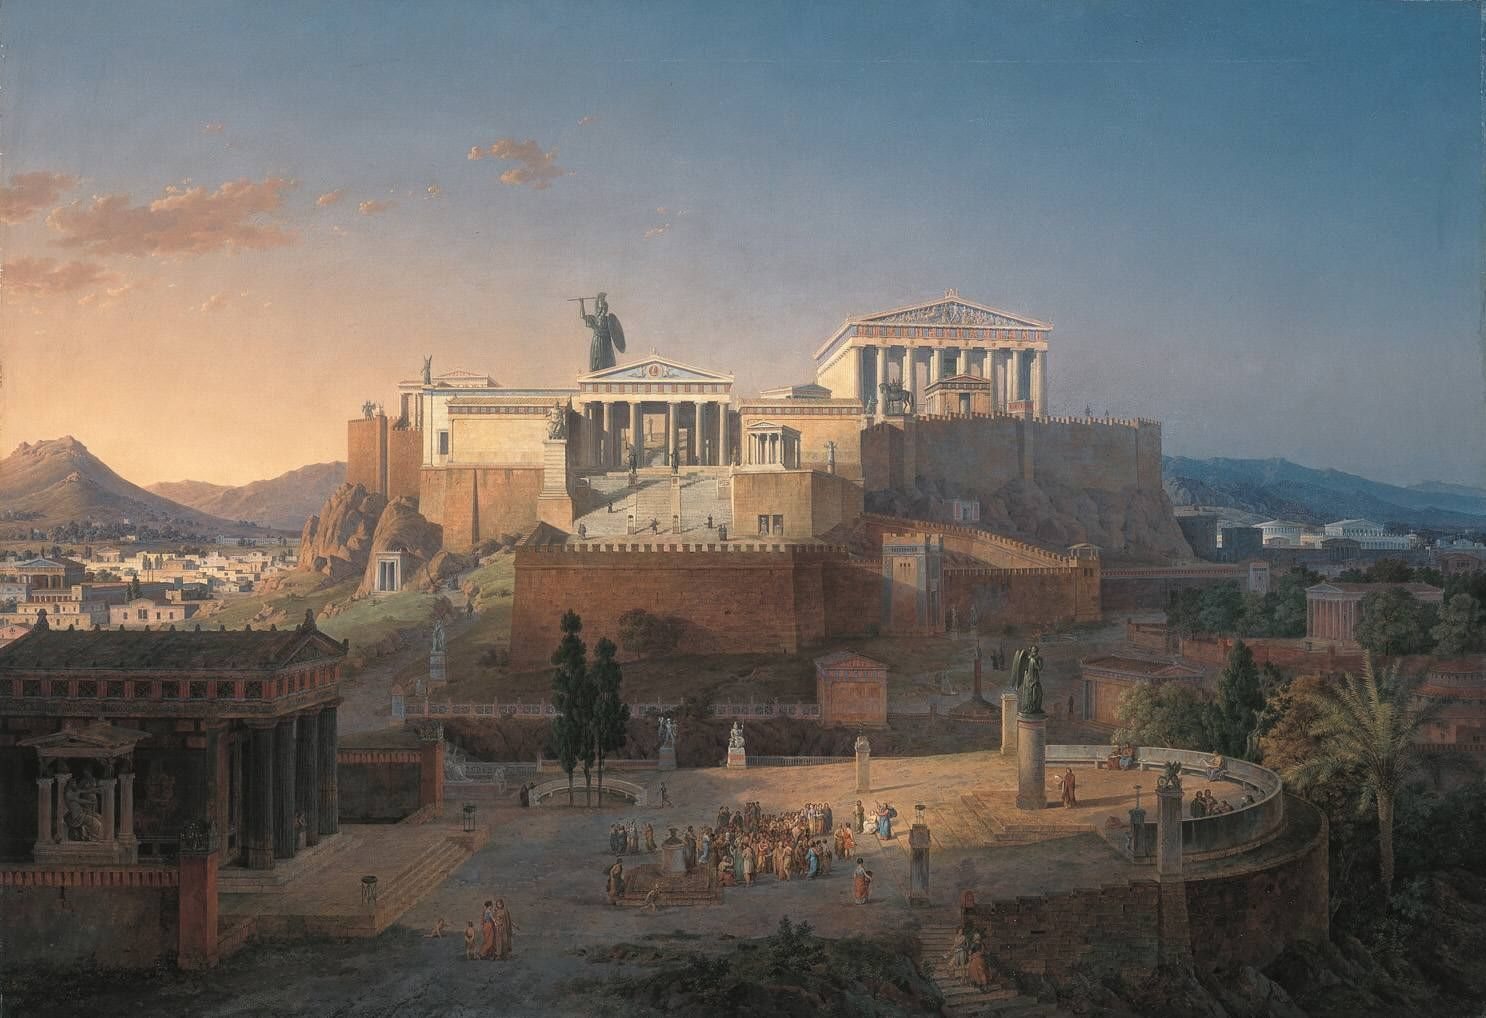
\includegraphics[scale=0.20]{graphics/Akropolis_by_Leo_von_Klenze.jpg}
     \caption{\emph{Acropolis of Athens}, Leo von Klenze, 1846, Neue Pinakothek, Munich}
     \label{acropolis}
\end{figure}

First, an acropolis is fortified. As the seat of political power it is prudential that it is. The sovereign divine revolutions are occupants of an acropolis and so are occupants of a fortified position. The skull of the head is the fortification of the immortal soul that is bound within. The thickness of the skull, and so the effectiveness of the fortification, is carefully balanced to optimize the intelligence of mortal beings. The thicker the skull, the better fortified, but the less room there is for marrow with which to bind the divine revolutions. The immortal soul is immortal. Strictly speaking, the fortification of the skull defends not the immortal soul but what binds it to the marrow of the skull. 

Second, an acropolis is typically located in an elevated position. There may be a number of reasons in play. In being elevated, the acropolis is closer to the divine and the intelligible, the source of its occupants' political authority. Being elevated is also a visible symbol of the political authority invested in the occupants of the acropolis. Finally, being elevated is an aspect of its extended fortification, in that an elevated position is easier to defend. At least the first two reasons are relevant to Timaeus' speech and possibly the third. Let us consider these in turn.

Perhaps the head is elevated so that it may be closer to the divine and the intelligible. The head, the acropolis of the immortal soul, is elevated in humans as opposed to beasts with four legs whose heads are directed downwards, towards the earth (91e). By contrast, the human head, in being elevated, may look, instead, to the Heavens and the intelligible. The head raises us up to kindred Heaven. In this regard, we are not like an earthly plant but a heavenly plant (90a). The Sun illuminates the wanderers so that we may see their motion (46e) and learn the art of number and perhaps even philosophy. The revolutions of the Heavens are divine thought made visibly manifest. In rationally attending to these in the right sort of way, we may perfect ourselves by assimilating to the divine. We are drawn to the divine and the intelligible through the Sun's illumination and this thanks, in part, to the Young Gods providentially providing the head with an elevated position in the human body. 

Timaeus hails from Locrus, but Plato having him describe the head in these terms may itself be the expression of a broader Athenian rationalism. Consider the following dramatic incident from Euripides' \emph{Heracles} (see figure~\ref{heracles}). Acting on Hera's orders, Iris has Madness drive Heracles in a frenzy in which kills his wife and children. Theseus, who Heracles rescued from Hades, encounters Heracles grieving with his mortal father, Amphitryon (Zeus, of course, being his immortal father). Amphitryon entreats Heracles to throw the mantle from his eyes and look to the Sun (\emph{Heracles} 1204--5). And Theseus, in a moving gesture of friendship, declares that he has no fear of pollution, and demands that Heracles unveil himself and look up (\emph{Heracles} 1225). Unveiling and looking up is to rationally attend to one's circumstance, and this is ethically significant. To fail to do so is ignoble even should one's circumstance be terrible as is the tragic situation that Theseus finds Heracles in. Rationally attending to one's circumstance is a kind of acceptance, and the noble soul endures divinely ordained misfortune and does not refuse them (\emph{Heracles} 1225). Euripides, like Timaeus, emphasizes that the head should be elevated, and there is a similar play with the divine, the intelligible, and the Sun's illumination. I am not claiming any specific influence here (though on the influence of Euripides on Plato see \citealt{Sansone:1996ux}). Rather, I claim only that Plato, in having Timaeus place the divine revolutions in the shining acropolis, gives specific expression to a broader Athenian rationalism.

\begin{figure}[htbp]
     \centering
         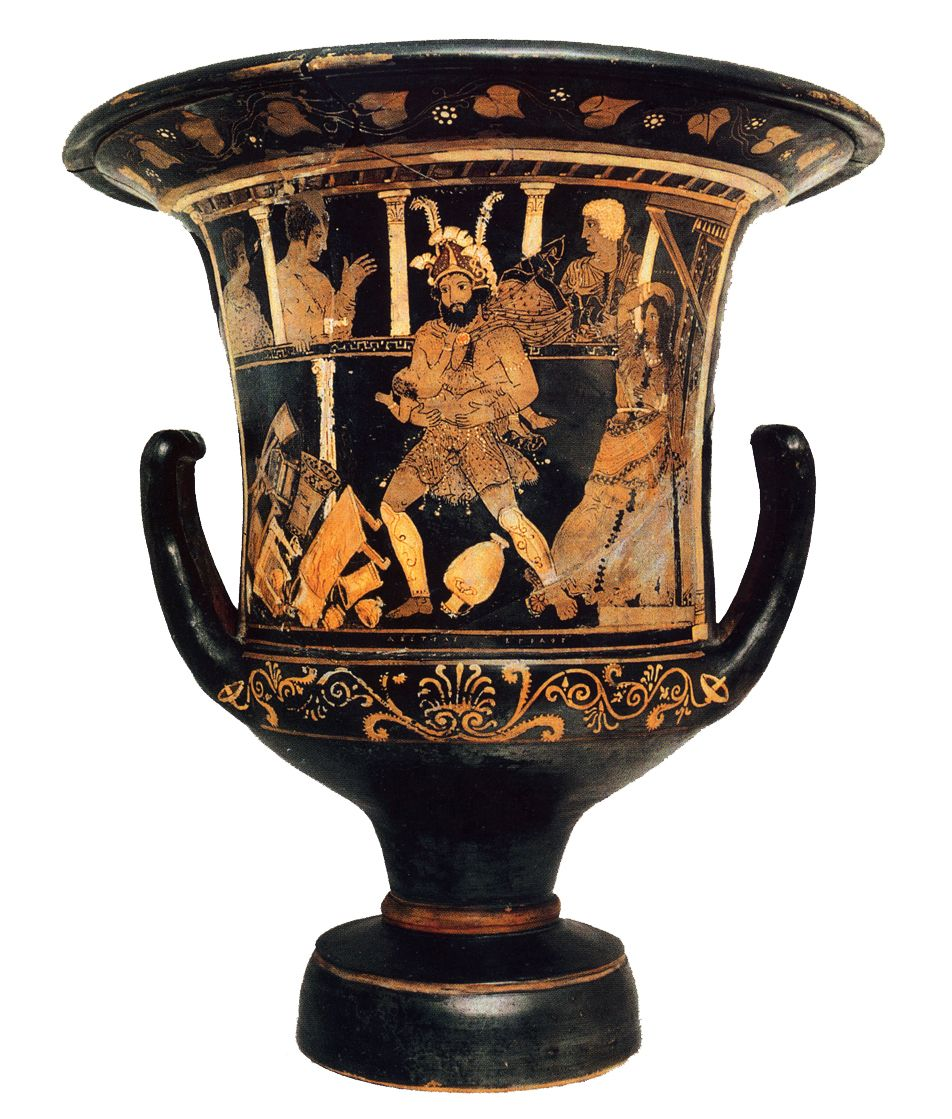
\includegraphics[scale=0.25]{graphics/heracles.jpg}
     \caption{\emph{Krater of the Madness of Heracles}, Calyx type, Side A, between 350 and 320 BCE, Museo Arqueológico Nacional, Madrid}
     \label{heracles}
\end{figure}

Perhaps the head is elevated as the expression of the political authority of its occupant. The immortal soul is divine and so suited to rule over the mortal soul and the body that it animates, and its being seated in the acropolis is an expression of its political authority. In demanding that Heracles raise his head, Theseus can be understood as exhorting Heracles to exercise rational control over his grief and regain his noble authority overthrown by grievous tragedy. The divine revolutions have political authority over the mortal soul and the body that it animates, and that its fortification is elevated is a visible expression of that political authority. 

Perhaps the head is elevated since an elevated position is easier to defend. If the third reason is in play as well, then elevation is an extended fortification. The head may be elevated to make it easier to defend from, say, low lying attacks from beasts on all fours. Thus, a dog may bite your hand or leg, but as long as you are standing, it cannot bite your head.

These three reasons are distinct, if complementary. I am inclined to believe that at least the first two are in play in Timaeus' speech.  I hesitate to endorse the third reason since Timaeus does not make it explicit. Like the utility of sight in navigating a complex and potentially dangerous environment, the benefit of an elevated position being easier to defend, if genuine, goes unmentioned.

There are two further aspects of the acropolis' fortification. Both may be described as parts of the extended fortification of the acropolis.

First, not only is the immortal soul bound in marrow encased in a hard skull in an elevated position, but it is separated from the region of the body occupied by the mortal soul. The head is separated from the trunk of the body by a narrow isthmus, the neck. If the hardness of skull and elevated position are meant to fortify against external attacks, the separation by means of a narrow isthmus is meant to defend against internal disruptions. Think of the disruptions of the cognitive revolutions occasioned by the \emph{pathēmata} of linear \emph{aisthēsis} in the shock of embodiment. While the immortal soul is divine, the source of these disruptions is corporeal, and Timaeus represent these as a form of pollution. (A potential point of contrast with Theseus who claims the divine does not fear pollution from mortals, but this is not the usual Greek view, and perhaps this is nothing more than a comforting lie directed towards the still grieving Heracles, \emph{Heracles} 1230.)

Second, just past the isthmus is stationed a barracks of guardians, the heart. The spirited part of the soul is the most receptive to the discursive commands of the divine revolutions. The heart is located just beyond the isthmus, in part, to better hearken to sovereign command. The heart may become inflamed because of an injustice perceived by reason. The source of the injustice may be internal as well as external and so, importantly, the heart also plays a policing role in keeping the unruly aspects of the appetitive soul in line so that they may not disrupt the divine revolutions of the soul. In these respects, in guarding against external and internal disruptions of the divine revolutions, the heart is part of the extended fortification of the acropolis.

% section reason (end)

\section{Spirit} % (fold)
\label{sec:spirit}

Just as the immortal part of the soul is separated from the mortal part by means of a narrow isthmus, the mortal part is itself divided. The mortal part of the soul is located in the thorax. The better part is separated from the worse part. The imagery shifts from a civic to a more domestic setting. Timaeus asks us to envision the better part separated from the worse part as a division separating the men's chambers from the women's chambers, perhaps by means of a screen. The imagery of containment persists. The better and worse parts of the mortal soul are contained as occupants in divided chambers. This division is the midriff or perhaps the diaphragm more specifically. In a passage overtly influenced by Timaeus, Aristotle describes the diaphragm as a partition (\emph{De partibus anamalium} 3.9 672b). Timaeus' description of this biological detail in terms of a common domestic setting signals, by way of contrast with the divine splendor of the sovereign acropolis, that we have moved from the ruler to the ruled. There may be another way in which the civic and domestic imagery interact. In portraying the broader \emph{polis}, where the majority of the population lives and works, as a domestic household Timaeus echoes and elaborates an aspect of the \emph{kallipolis}---that the citizens of the \emph{polis} are encouraged to think of themselves as family. And, as Timaeus elaborates, since the citizens are family, then within the \emph{polis} they are occupants of a common domestic household. Furthermore, the domestic setting, a household separated into two chambers by means of a screen, must be read as a description of the broader \emph{polis} since civic structures of that \emph{polis}---the barracks of the guardians, the manger---are located within these chambers. The civic and the domestic imagery are in this way interdependent.

Spirit, the better part of the mortal soul, is housed in the men's chambers. These are nearer to the isthmus bordering the grounds of the acropolis. So the men's chambers in which the better part of the mortal soul is housed is the upper thorax, above the midriff or diaphragm. (For reasons that he declines to state, \citealt[257 n13]{Archer-Hind:1888qd}, denies that there is a fact of the matter concern which chambers, the upper or the lower, is the men's chambers and which is the women's. See \citealt[501]{Taylor:1928qb}, for criticism.)

Spirit animates social passions aimed at competitive advantage. Timaeus describes spirit as a love of victory. The spirited part of the soul is placed in the upper thorax so that it may better hearken to reason. Despite animating social passions and so being fundamentally other regarding, the primary ethical function assigned to spirit involves maintaining order within the psychic \emph{polis}. In the virtuous at least, spirit hearkens to reason and so joins with it in putting down the unruly tribe of desires, the worse, appetitive part of the soul, located at a safe distance from the acropolis, in the lower thorax, below the midriff or diaphragm.

Within the men's chambers that houses the better part of the mortal soul---the upper thorax---the Young God's place the heart. The heart is the primary organ associated with spirit. The primary organ associated with a part of the mortal soul is the corporeal instrument of the ethical function of that part. The heart is described as a knot of veins and a fount of blood that circulates through the limbs. This is a reasonably accurate if curiously generic description. Thus, for example, Timaeus seems not to mark the distinct roles of veins and arteries. However, Timaeus is not, here, primarily interested in the heart's role in the circulation of nutriment. Rather, Timaeus is more concerned to place the heart in the political topology of the mortal soul and to explain how it may be the corporeal instrument for the rational oppression of the unruly tribes of desire when they fail to heed the commands of the sovereign acropolis.

The Young Gods place the heart in the upper thorax. The men's chambers must really be understood as a region of the psychic \emph{polis}, adjacent to the isthmus separating the acropolis. Timaeus describes the heart as the barracks for guardians. So these barracks are in the upper region adjacent to the isthmus but are not their sole occupants. The lungs, the secondary organs of spirit, are also located in the men's chambers. A secondary organ associated with a part of the mortal soul is a corporeal instrument that serves an auxiliary role in the exercise of the ethical function of the primary organ. The secondary organ maintains and regulates the primary organ so that it may better exercise its ethical function. The lungs are only in a position to do so by cohabiting the men's chambers with the heart.

The heart's being described as a barracks highlights its ethical function. The barracks are located near the isthmus so that the discursive commands of the immortal soul are better heard. Again, the isthmus may separate, but it is so designed that there is a line of communication between the acropolis and the barracks of the guardians. The guardian's reception of discursive commands is described in terms of audition. And not any form of audition, but one of the special forms of audition involved in Timaeus' sensory soteriology (47c--e). We may better harmonize with the revolutions of the World Soul by listening with rational attention to music or rational speech. The guardians housed in the barracks listen with rational attention to the discursive commands of the immortal soul housed in the acropolis.

How are we to understand the communication between the immortal and mortal parts of the soul? Does the occupant of the acropolis merely issue sovereign commands or does it also receive reports on what transpires within the broader \emph{polis}? It is clear that the commands of the immortal part of the soul are discursively articulated. In understanding these commands, in whatever sense that they do, do the mortal parts of the soul receive discursive contents that they can understand? As we shall see, at least for the worse part of the mortal soul, it seems the answer is no. From the commands of the immortal soul being discursively articulated we may not conclude that their reception is itself discursively articulated. Even someone who denies that dogs have the power of speech will readily concede that there is some sense in which they understand and heed their master's discursively articulated commands. Understanding the nature of such communication is important for the topic of the present essay, the nature of perception. Perceptual powers are powers of the mortal soul and perception only occurs when it is reported to the \emph{phronimon}, a part of the rational, immortal soul. So the nature of the report or channel of communication bears on whether or not the content of perception is best conceived as discursively articulated. We shall return to this important issue after discussing the worse part of the mortal soul, appetite.

The heart is assigned as the barracks of the guardians so that it may discharge its ethical function as the primary organ of spirit. Indeed, the civic description, as barracks of the guardians, vividly expresses its ethical function. Guardians guard against external and internal threats to the \emph{polis}. The ethical function of the heart is triggered when reason passes word around that an unjust action affects the \emph{polis}, whether the agent of this injustice is external or internal, such as the unruly desires that can fail to heed to reason. The heart only begins its work when it receives such word. So the report of an external or internal injustice that affects the \emph{polis} is issued from the acropolis and its reception sets the heart in motion. It is unlikely, then, that the word is passed around by means of the heart's vigorous circulation. Upon the receiving word of an injustice that affects the \emph{polis}, the heart becomes inflamed. The inflammation of the heart is really only an auxiliary cause of the exercise of its ethical function, the real cause is the realization of the end, the ethical function itself. The heart, when inflamed, heightens the senses. It does so by vigorously circulating hot blood through the blood vessels (\emph{phlebes)} extending throughout the body. Thus \citet[503]{Taylor:1928qb} writes ``The royal `guards' are thought of as making their way into all the narrow alleys of the city to quell a disturbance''. It might be natural to think that since the heart is inflamed every instrument of perception is more readily affected by its object so that the agent of the unjust activity may be more readily perceived. But that is not what Timaeus actually says. According to Timaeus, the heightened sensitivity is for the sake of receiving commands of reason and threats of sanction lest they fail to obey those commands in every instance. The heart marshals the powers of the mortal soul so that the mortal soul and the body that it animates should follow the leadership of the best part, so that the agent of the injustice that affects the \emph{polis} may be appropriately dealt with. The heightening of the senses is not, then, best understood as the increased sensitivity of specifically the instruments of perception. Recall that \emph{aisthēsis} is sometimes understood narrowly as perception or sensation. But, importantly, it is sometimes understood more broadly to include the unruly desires of appetite. Like perception, such desires have corporeal instruments subject to \emph{pathēmata}. So the heightening of the senses is better understood as vivification more generally. Moreover, their heightened sensitivity is not to their objects, what the corporeal instruments typically measure, but to the sovereign commands of reason and threats of sanction in light of noncompliance. 

If the heart is the primary organ of the spirited part of the mortal soul, then the lungs are the secondary organ of spirit. The secondary organ is an auxiliary organ that maintains and regulates the primary organ so that it may better execute its ethical function. In the case of the lungs, its auxiliary function as secondary organ of spirit is to cool the heart when overheated. More specifically, when danger is expected passion is excited and the heart leaps because of the increased presence of fire. And the lungs are meant to cool the heart in these circumstances. While the heart may be inflamed in the presence of danger, it should not when the danger is merely expected. Timaeus does not explicitly say why, but one may reasonably speculate. In the presence of an external threat, the inflammation of the heart vivifies the mortal being so that they may more effectively deal with the threat. But when the threat is merely expected, the inflammation of the heart may lead to excessive anxiety and even cowardice. Nevertheless, due to its corporeal nature, the heart tends to become inflamed even in these circumstances. The lungs function so as to regulate any such excessive overheating of the heart so as to prevent any adverse effects.

The lungs are soft and bloodless. Presumably, they are soft so that the heart does not suffer from its repeated collision with them when it is leaping. The lungs, being soft, yield to the leaping heart and so function as padding. That the lungs are bloodless means that the heart is not circulating hot blood to them when it is overheating, and so the lungs are not thereby hindered from their cooling role. The lungs have the structure that they do in order to subserve this cooling function. The lungs are filled with perforated cavities like a sponge. This is so that it may better receive air and water so that it may cool the heart. Not only does this regulate the heart's activities, but it also offers it relief and comfort. In ordered for the perforated cavities of the lungs to be filled with air and water so that it may cool an overheated heart, the channels of the windpipe were drawn so that it may receive breath and drink. The lungs may not have been given a civic description of its location within the \emph{polis}, other than being cohabitants, with the heart, of the men's chamber, but if the windpipe is to receive breath and drink, it must extend along the narrow isthmus since breath and drink are received in the head, through the nostrils and the mouth. When danger is expected and the heart leaps from fear, the heart collides with the soft padding of the lungs which yields to the heart and cools it so that it may better answer to reason.

If the lungs are an auxiliary organ to the primary organ of spirit, the heart, then the windpipe is an auxiliary organ to the secondary organ of spirit, the lungs. The ethical significance of the lungs derives from the ethical significance of the heart's proper functioning that it maintains and regulates. Similarly, the ethical significance of the windpipe, entirely derives from aiding the lungs in their cooling role and their own derivative ethical significance. Timaeus is only here concerned with the lungs as an auxiliary of the primary organ's ethical function. Nothing is said about their biological function apart from their cooling the heart. 

Moderns will be especially surprised given that we believe that the lungs contain blood vessels and that respiration is the primary biological function of the lungs. Let us briefly consider these worries in turn. 

First, while Timaeus claims that the lungs are bloodless, they in fact contain blood vessels. Aristotle will criticize the opinion that the lungs are bloodless in \emph{Historia animalium} (496b). Timaeus, though, does not seem to be his primary target so much as the medical tradition that Timaeus may have been drawing upon. For one thing, Aristotle attributes this error to the over-reliance on observations based upon dissections since the animal exsanguinates upon death. Timaeus, however, gives no indication that he has so much as witnessed a dissection. 

Second, not only is no mention of respiration made here, but some of what Timaeus claims can seem incompatible with respiration as we conceive of it. The lungs cool the heart, in part, by being filled with water. Timaeus' claim, here, is at best accidentally true, but not in a way that will allow the lungs to discharge their assigned auxiliary role. It is true that the heart will cool by filling the lungs with water, but only as a result of death by drowning. According to Timaeus, the lungs are filled with water that it receives from the windpipe. Aristotle also argues against the opinion that the windpipe receives water in \emph{De partibus anamalium} (3.3 664b), though, here, Timaeus is plausibly an explicit target. Aristotle advances a number of empirical considerations against this opinion. Thus we may observe the choking, distress, and violent coughing that results when nutriment is lodged in the windpipe, be that nutriment solid or liquid. Furthermore, we observe that when we vomit, liquid is not discharged from the windpipe, but rather from the oesophagus that leads to the stomach. The lungs do not lead to the stomach, and so there is a puzzle about how the liquid filling the lungs is consumed. Moreover, it is evident that liquid nutriment first accumulates in the stomach before moving to the bladder.

One final remark about the political topology of spirit. Just as the divine part, the immortal soul, is the occupant of the acropolis, are we to imagine that spirit occupies, as well, the barracks of the guardians? Spirit, then, would not just be located in the upper thorax, but in the heart more specifically. And though spirit is personified as a guardian in executing the ethical function of the heart, there is reason to doubt that spirit is confined to the heart. The heart is the primary organ of spirit. The secondary organ plays an important auxiliary role in maintaining and regulating the primary organ so that it may better execute its ethical function. What animates the lungs, the secondary organ, so that they may cool the heart when overheated? Plausibly the mortal soul. But if the mortal soul animates the lungs by being present to it, then its presence is not confined to the heart. So despite the dramatic personification of spirit as a guardian of the \emph{polis}, spirit is not confined to the heart. The heart is merely the corporeal instrument of spirit when playing the role of guardian in the psychic \emph{polis}.

% section spirit (end)

\section{Appetite} % (fold)
\label{sec:appetite}

If spirit animates social passions aimed at competitive advantage, appetite is that part of the mortal soul that animates desire for nutriment and any other desire grounded in our corporeal nature. Appetite, the worse part of the mortal soul, is placed in the women's chambers, midway between the midriff or diaphragm and the navel. The region of the body dedicated to the feeding of the body is described as a manger. Just as the immortal soul is the sovereign occupant of the acropolis, appetite is at the trough in the manger. Appetite is described as savage, bestial, and bound and is only joined to the rest and fed since it is necessary for mortal existence (compare \emph{Republic} 9 588c7). Appetite is plural. It is appetitive desires that are savage, bestial, and bound. Appetite animates a plurality of desires reflecting the plurality of ways a body may be affected in the realm of Becoming. The manger has the relative location that it does, located as far away as possible from the acropolis, in order that the acropolis remain free as possible from turmoil and din. The sounds of the unruly beasts bound in the manger are \emph{amousikē}. Recall, that \emph{mousikē} is adapted to sound and hearing is given for the sake of \emph{harmonia} (see chapters~\ref{sec:the_end_of_audition} and~\ref{sec:the_ears}). Notice that the turmoil and din of the unruly tribe of desires is not rationally ordered and, far from promoting or even preserving \emph{harmonia}, has a tendency to disrupt the harmonic revolutions of the the immortal soul if within earshot of the acropolis. Thus in order for the supreme part of the soul to take counsel in peace concerning what benefits one and all, the manger in which the savage beasts are bound at the trough is far removed from the sovereign acropolis on high.

Given appetite's association with nutrition, one might have expected that the primary organ of appetite would be the stomach. And though Timaeus provides us with an ethically loaded description of the biological function of the stomach in digestion and nutrition, it is not the primary organ of appetite. The primary organ of appetite is, instead, the liver. Why this curious substitution?

Timaeus offers an explicit reason from the start. This concerns the cognitive limitations of at least this part of the mortal soul that affect the means by which it may communicate. Appetite does not understand reason though it has a share in the perception of reasons (71a3--4). Later, Timaeus emphatically repeats the point---appetite has no part of reason and intelligence (\emph{logou kai phronēseōs}, 71d4). Appetite is not naturally inclined to pay heed to the discursive commands of reason and is easily distracted by the play of images and phantasms (71a4--6). Appetite is incapable of understanding rational speech. There is a failure of communication. The discursive demands of reasons are neither heard nor heeded. They are not heard in the sense of listening with rational attention to intelligible structure, the kind of listening that gives rise to, not pleasure (\emph{hēdonē}), but delight (\emph{euphrosunē}). Importantly, this applies to listening to rational speech as much as it does to listening to music. This is important since the demands of reason are persistently represented as being communicated through rational speech. We are to imagine the sovereign commands of reason articulated in a booming announcement from the acropolis directed to the broader \emph{polis} spread out below. For the inhabitants below, hearing well might involve stopping what they are doing and looking up to the source of the announcement, the sovereign acropolis, so that they may better understand the intelligible structure of sovereign speech. While the discursive demands of reason are not heard in this sense, appetite is not utterly insensitive to reason. Perhaps, the experience of appetite when subjected to rational speech is like the experience of a person listening to someone speak a language that they do not understand. Though they may hear the foreign speech they are not in a position to rationally attend to its intelligible structure. Being without reason and intelligence, appetite cannot rationally attend to the intelligible structure of reason's sovereign commands and is naturally indifferent to them.

This communication breakdown is providentially provided for, however. To accomodate appetite's inability to understand the sovereign commands of reason, God placed the liver in the dwelling of this part of the soul. How we are to understand this depends upon whether the manger is the whole of the women's chambers, the lower thorax, or the manger is a civic structure contained within the women's chambers. On the former hypothesis, Timaeus is claiming that the liver is an occupant of the manger. On the latter hypothesis, it is at least open to understand Timaeus as claiming that the liver merely dwells in the women's chambers, perhaps adjacent to the manger. This latter reading receives some support from the fact that Timaeus' descriptions of the occupants of the manger---savage, unruly beasts that produce a tumultuous turmoil and must remain safely bound---seem inappropriate, as we shall see, when applied to the liver. Moreover, Timaeus' imagery shifts from the civic to the domestic. The liver is not likened to any civic structure but to a mirror, an item to be found within in women's chambers of domestic households. Just as a mirror may dwell within the women's chambers, perhaps the liver, with is smooth, mirror-like surface, dwells within the women's chambers, the lower thorax.

God placed the liver in the dwelling of this part of the soul as an alternative non-discursive mode of communication so that appetite may better understand and heed the commands of reason. While appetite may not be able to receive discursive contents that it can understand, it remains susceptible to visual contents. Images and phantasms (\emph{eidōlōn kai phantasmatōn}) capture the attention of appetite, and appetite subsequently has the tendency to follow their lead. God exploits this tendency of appetite for the better by placing the liver to dwell along with it. Thanks to its smooth surface, the liver can receive rational images, the way mirrors can receive visual images. So appetite's failure to receive the discursive commands of reason is compensated by liver's capacity to receive rational images. Such imagery provides the appetite non-discursive contents that it can apprehend. Moreover, as we shall see, such imagery affects the liver, and the mortal soul more generally, in such a way as to give rise to pain and pleasure and hence to affective states that depend upon these such as fear. In this way, through a play of imagery that gives rise to pain and pleasure, reason can motivate appetite to heed the demands of reason. Heeding, here, is, in Kantian parlance, appetite's acting in conformity with reason as opposed to acting from reason (since the latter requires reason's demands be discursively understood). Subsequently, the providential gift of the liver is described as the organ of divination that allows the worse part of the mortal soul some measure of truth. 

Timaeus begins by describing the corporeal composition of the liver and then the painful and pleasurable images that may be received from reason. The pain and pleasure that accompanies rational imagery is the means by which reason may influence appetite and the body that it animates. Why the liver should have the corporeal composition that it does emerges in Timaeus' account of the pain and pleasure of rational imagery.

The liver is dense (\emph{pukron}), smooth (\emph{leīon}), bright (\emph{lampron}), and sweet (\emph{gluku}) yet containing bitterness (\emph{pikrotēta}). These are all sensible features and, as the sensible is the mark of the corporeal, features that only bodies may have. That it is dense, smooth, and bright make it receptive to rational images the way that mirrors are receptive of visual images. That it is sweet and yet contains bitterness is the means by which appetite is motivated by the occurrence of rational imagery. Let us consider these in turn.

First, the liver is dense (\emph{pukron}), smooth (\emph{leīon}), and bright (\emph{lampron}) (compare the discussion of images in the Divided Line where bodies that receive images are similarly described as dense, smooth, and bright, \emph{Republic} 509d6--510a3, though \emph{phanron} is used for bright instead of \emph{lampron}). These sensible features are what make the liver receptive of rational imagery. The liver is explicitly compared to a mirror. What about a mirror makes it receptive to visual images? In his catoptrics (46a3–46c6, discussed in chapter~\ref{sec:timaen_catoptrics}), Timaeus told us that mirrors, such as a highly polished piece of bronze (see figure~\ref{bronze_mirror}), are reflective and smooth (\emph{emphanē kai leia}). Not every surface is receptive to images, only surfaces that meet certain conditions, and being reflective and smooth are conditions on a surface's receptivity to images. Smoothness is a matter of degree, and the greater smoothness the greater the clarity of the image. The smoother the surface the greater the resolution. But smoothness is not just a prerequisite for the reception of clear images, but to the reception of any image at all. Consider a smooth surface in which an image is reflected. Imagine it becoming increasingly less smooth until it is rough. The clarity of the reflective image will decrease, but when the surface is rough the image will no longer be reflected. It is unsurprising, then, that Timaeus describes both mirrors and the liver as smooth. 

\begin{figure}[htbp]
     \centering
         \includegraphics[scale=0.09]{graphics/bronze_mirror.JPG}
     \caption{\emph{Mirror with Siren}, 450-400 BC, Greek, Locri Epizephirii, necropolis, Lucifero district, bronze,Cleveland Museum of Art}
     \label{bronze_mirror}
\end{figure}

Their are however verbal differences between Timaeus' catoptrics and his description of the liver. Whereas the mirror is reflective (\emph{emphanē}) the liver is dense (\emph{pukron}) and bright (\emph{lampron}). 

Let us begin with density, first, since it is probably related to the liver's smoothness. The liver is dense in the sense that the material that composes it is closely compacted. This is presumably a corporeal condition on smoothness since if the material that composes the surface is only loosely compacted that surface will be rough. So the occurrence of density in the account of the liver merely elaborates the earlier catoptrics by drawing attention to density as a precondition for smoothness. 

A close look at \emph{emphanē} and \emph{lampron} show that the are not unrelated. I have translated \emph{emphanē} as reflective but taking account of the prefix and root of the word it more literally means visible in or in which something is visible. \emph{Phanē} means a torch or a lantern or the light that they emit. It is common in Greek, however, for words with that root to mean visibility as opposed to the light by which we see. So in being \emph{emphanē}, things are visible in that surface. But even here both meanings may be in play. Things are visible in a surface because it is receptive to light, in particular the chromatic fire emitted by the body seen in that surface. Indeed, this is not the first time we have seen Timaeus make simultaneous play of \emph{phanē} meaning light or sight. On Timaeus' understanding of \emph{diaphanē}, it is only if the visual body, \emph{opsis}, shines through does the perceiver see through the diaphanous body, discussed in chapter~\ref{sec:the_eyes}. If that is right, if a body is visible in a surface only if it is receptive to the chromatic fire emitted from that body, then this coordinates well with the later description of the surface as bright (\emph{lampron}). Further, recall that an experience of \emph{lampron} is an experience in which all kinds of colors may appear. Similarly, an experience of a mirror is an experience in which all kinds of colors may appear. Indeed, it is because all kinds of colors appear in mirrors that they can quickly and easily produce images of everything in the sensible Cosmos as Socrates observes (\emph{Republic} 596d8--e3.) So despite the verbal differences between the sensible features of the liver and the mirror, there is no substantive departure from the principles of Timaean catoptrics.

The two other sensible features of the liver, sweetness and bitterness, do not explain the power to receive rational imagery so much as they are the potential effects of the reception of such imagery. Timaeus claims that the liver is sweet and yet contains bitterness. This strongly suggests that the liver is in its natural state when sweet, and that the liver only becomes bitter when it departs from that natural state. Recall that sweetness restores the the tongue to its natural state and all the other flavors involve different determinate departures from that natural state. Moreover, while pain involves a departure from the natural state of the body, pleasure involves a return to that natural state. So the sweetness and bitterness of the liver will be the means by which appetite will heed what it is otherwise indifferent to. 

One final remark about Timaeus' language here. The liver is sweet and yet contains a share of bitterness. What does Timaeus mean by this? After all, if something is white if potentially black we do not normally say that it is white and yet contains a share of blackness. Timaeus does not seem to be claiming that while the liver is predominantly sweet it has some bitterness mixed in. I think instead we are meant to imagine that the liver has reservoirs of sweet and bitter substances that may suffuse the organ making itself sweet or bitter if is acted upon in the right sort of way. Why otherwise say that the liver contains bitterness as opposed to saying that the liver is sweet and yet may become bitter?

The liver's reception of rational imagery is described in two ways, depending upon whether the reception of these images gives rise to pain or pleasure. 

First, the powers of thought proceed from the understanding and the liver receives impressions of these the way that mirrors receive visual images. The analogy, here, is to the mirror's reception of a visual image, not to the appearance of the object of that image to a perceiver looking into that mirror. Suppose that the image in a mirror is of some nearby colored body, then that image is formed from chromatic fire emitted by the body gathering upon that mirror. It is on the surface of the mirror that the visual body, composed of the internal fire of the eye and brother daylight, meet the chromatic fire, and this is where the chromatic fire acts upon the visual body. When this affection is reported to the \emph{phronimon}, the image is cognized and the colored body is visible in the mirror. The formation of images in mirrors presently at stake is the chromatic fire received on the surface of the mirror, and not the body's perceptual appearance. This is significant, since if the analogy is thus understood, then reception of the impression of the powers of thought is like the reception of illumination---if not of daylight, then chromatic fire. If this seems odd to you, perhaps due to an inability to bracket what we know about catoptrics, consider a bright yellow ball next to a white wall on a bright sunny day. The ball will reflect its yellow color on the wall. Might this not, in the fifth century at least, be plausibly described along Empedoclean lines, as the emission of chromatic effluences? 

Second, when describing the pleasurable effects of the images and phantasms received from reason, the imagery shifts from illumination to inspiration. Instead of the powers of thought proceeding from \emph{nous} being likened to chromatic fire being emitted from a colored body, they are now likened to gentle speech, like a mother's trying to soothe a pre-verbal infant held in her lap. Specifically, it is the mild breath of \emph{nous} that portrays phantasms on the liver's surface. Timaeus has moved from the visible to the audible and, if the mild breath of \emph{nous} may be felt upon the liver's surface, the tangible. 

How are we to understand these two different descriptions? Must they be understood as competing?

First, notice that it is \emph{nous}, a power of the immortal soul, that is said to act upon the liver. There is no suggestion, here, that the powers of thought proceeding from \emph{nous} are mediated by spirit directly dealing with the liver in the noisy neighboring chambers. Spirit's lack of involvement is odd since the end of the rational imagery is to encourage appetite to heed the demands of reasons. So described, however, that seems like the role of the guardians, not the sovereign. 

Second, notice that neither the illuminationist nor the inspirationist description can be understood literally. \emph{Nous} does not illuminate the liver. All is dark within. Even if an intracorporeal light should shine from the head down upon the liver, its progress would be blocked by the heart and the lungs and any other intervening organs. Nor is the liver's surface subject to a gentle breeze. Against any sea breeze from the acropolis channeled through the isthmus out onto the broader \emph{polis}, the heart and the lungs and the other intervening organs stand as bulwarks, like intervening mountains. So Timaeus has not provided us with descriptions of the causal mechanism involved in the liver's formation of images. If there is a point to the imagery of illumination and inspiration, it must concern not physiology but psychology. 

I am inclined to think that the first illuminationist description, where reason acting upon the liver is likened to a body emitting chromatic fire upon a mirror's surface, is meant to hold generally. That is, it is meant as a description of image formation in the liver when the rational imagery causes pain as well as when it causes pleasure. The second inspirationist description, however, is specific to the second case where the reception of rational imagery helps restore the liver to its natural state and so gives rise to pleasure. On this interpretation, the descriptions are not competing but stand as a description of a genus does to a description of one of its species.

The action of \emph{nous} upon the liver produces painful and pleasurable effects. Timaeus considers the painful case first and then the pleasurable case. Why in that order? First the reception of rational imagery that gives rise to pain is the means by which reason threatens appetite and so coerces compliance with its demands. Perhaps pain comes first since it is necessary to redress appetite's inability to understand the discursive demands of reason. There may be an additional, complementary reason in play. The mild breath of reason may soothe the liver so as to give rise to pleasure, but only once the liver has departed from its natural state. In describing the case of pain first, Timaeus details all the relevant ways in which the liver may depart from its natural state. Moreover, these are ways that need to be restored, somehow, by rational imagery of another kind. So the two cases are ordered by ethical significance and by the demands of physiological exposition.

When the powers of thought proceed from \emph{nous}, the surface of the liver receives impressions the way a mirror receives visual images. The images received may frighten the liver. Presumably it is the objects of these images that frighten the liver. Imposing frightening imagery upon the liver is reason's means of issuing a stern threat when appetite pays no heed to its demands. A primary effect of the frightening imagery imposed by reason is for bitterness to suffuse through the substance of the liver which in turn gives rise to a number of secondary effects. Thus when the bitterness suffuses through the substance of the liver, the liver takes on a bilious color (the color of bile, a yellowish or greenish color), it becomes compressed so that its surface becomes wrinkled and uneven, and its lobe curls and shrivels and passages are compressed and closed causing pain and nausea.

When the mild breath of \emph{nous} portrays images of the opposite kind, the liver may be restored to its natural state. The images are of the opposite from the kind that frighten the liver. Again, presumably this concerns the objects of these images, what they image. No longer being subjected to frightening imagery, the bitterness of the liver begins to calm down. Thus the frightening imagery not merely caused but sustained the bitterness of the liver. And just as frightening imagery on the smooth surface of the liver causes bitterness inherent in the liver to suffuse throughout its substance, imagery of the opposite kind causes sweetness inherent in the liver to suffuse throughout its substance. That sweetness suffuses throughout is the primary effect of such imagery. Sweetness has a restorative effect and the secondary effects concern this. The curled and shrivelled lobe straightens, the wrinkled surface of the liver becomes smooth again, and the compressed and blocked passages become free. The liver is thus restored to its natural state. Moreover, and importantly, the pleasurable effects are not confined to the liver itself. The surrounding parts of the soul become gracious and cheerful in response to the liver being restored to its natural sweetness. So not only does the liver respond to the suffusion of its inherent sweetness the way that the tongue responds to sweetness, but the surrounding parts of the soul respond in this way as well to the sweetness of the liver. 

Just as the pleasurable effects are not confined to the liver but extend to the surrounding parts of the soul, plausibly the painful effects are not themselves confined to the liver but extend, as well, to the surrounding parts of the soul. Moreover, they would have to, if reason is aiming to get appetite to heed its demands with stern threats. If the painful effects are only confined to the liver, it is merely the liver that is threatened and not appetite more generally. Moreover, the pain and nausea caused by the blocked passages of the liver are not confined to the liver but extend to the surrounding area. So though Timaeus is more explicit about the pleasurable effects extending to the surrounding parts, the same must hold, as well, for the painful effects.

By means of a play of painful and pleasurable images, reason coerces appetite to heed its demands. This regulative role of the liver should be distinguished from its divinatory role. The source of the imagery are different in the liver's regulative role and in its divinatory role. In its regulative role, \emph{nous} is the source of imagery. \emph{Nous}, here, is the noetic faculty of the immortal soul. It is not the noetic faculty of the World Soul. Nor is it the Demiurge who is associated with \emph{nous} (for discussion, see \citealt{Menn:1992ez}). This is important since in the liver's divinatory role, \emph{nous} is not the source of imagery but \emph{to theion} is. So these roles may be distinguished since the source of the liver's imagery is different in each. 

The benefits of vision include the art of number, the concept of time, and even philosophy, but none of these are the \emph{aitia} of vision (47b5--c4). Instead, cognitive assimilation to the Cosmic God is that for the sake of which the Young Gods endow mortals with eyes to see with. Similarly, the regulation of appetite is a benefit of the liver, but it is not the \emph{aitia} of the liver either. Instead, divination is that for the sake of which the Young Gods endow mortals with a liver. The Demiurge enjoined the Young Gods to make the mortal part as good as possible. Thus the part of the body inhabited by appetite is redeemed by making it a site of divination, and so having a share in truth. Moreover, having a share in divinely revealed truth is a greater benefit than being coerced to heed to demands of reason by a play of painful and pleasant imagery.

Timaeus is drawing upon and criticizing a traditional practice of using liver in rites of divination. Thus the livers of sacrificed animals were examined and a prophecies were made given their observed state. Thus Aegisthus examines the liver of a calf sacrificed by Orestes and discovers an ill omen:
\begin{quote}
	Aegisthus took the entrails in his hands and carefully examined them. Now the liver had no lobe, while the portal vein leading to the gall-bladder portended a dangerous attack on him who was observing it. Dark grows Aegis\-thus' brow \ldots\ (Euripides \emph{Electra} 827ff; E.P. Coleridge in \citealt[92]{Oates:1938la})
\end{quote}
From this practice, Timaeus retains the liver as the site of divination. Moreover, in each case, the liver may be the site of divination, but its source is divine. Timaeus also retains the distinction between the state of the liver, on the one hand, and the prophet who interprets the state of the liver, on the other. Despite accommodating these insights, Timaeus is nonetheless critical of the traditional practice of using sacrificial livers in rites of divination. He asserts that the liver is better suited to divination when alive.

The liver receives divinatory imagery when the mortal being is asleep and reason is fettered. Timaeus is keen to emphasize that the power of divination is linked with the incapacity of reason. He does so by emphasizing two distinct roles in any rite of divination. On the one hand there is the recipient of divine inspiration. On the other hand, there is the interpreter of the divinely inspired speech or vision. The recipient of divine inspiration is rationally incapacitated---by sleep, or sickness, or by some change induced by possession. The interpretation of the divinely inspired speech or vision is, by contrast, a rational activity. No one person may play the both roles at the same time. Thus someone may have a divinatory dream, say, but they can only interpret it when awake, the dream remembered, and reason unfettered.

How does Timaeus account of divinatory dreams cohere with his earlier account of mundane dreams more generally. In the earlier mundane account, the imagery involved in a dream arises in the calm motion of the eye's fire. In the later divinatory account, the imagery arises in the smooth, mirror-like surface of the liver. In the earlier account, the medium of the image is dynamic---the calm motion of the eye's fire. In the later account, the medium of the image is static---the smooth surface of the liver. In the earlier account, the cause of the imagery was endogenous. In the later account, the cause of the imagery is exogenous. 

One way to reconcile these accounts is to attribute to Timaeus the view that there are different mediums of dream imagery governed by different mechanisms. The imagery of mundane dreams arise in one medium by one kind of mechanism. The imagery of divinatory dreams arises in a different medium by a different mechanism. The accounts are made to cohere by understanding them as having different, if related, subject matters. If we allow that we may be in doubt whether a dream is divinely inspired, that means that the imagery in different mediums that result from different mechanisms may be sufficiently alike for this to be possible. Perhaps so. But it is at lest unobvious that images in the calm motion of fire are very much like images in impressions on the surface of a liver, and Timaeus provides no assurance that divine dreams may be indistinguishable from the mundane in this way. There may, however, be other ways in which the accounts may cohere. 

Perhaps we are missing the genus for the species. Perhaps the medium of dream imagery is vital motion, broadly understood, that may be cognized by the soul. The qualification is important. Should vital motion occur surrounded by immobile parts, it may not reach the soul and so go uncognized (as when we fail to feel our nails grow). Both the calm motion of the eye's fire and the play of impressions across the liver's surface count as vital motion in the intended sense. The play of impressions counts as motion broadly understood. And it is vital in that the impressions play across the liver of a living being. Only the living are suitable to receive divine inspiration. The calm motion of the eye's fire is vital as well. The eyes dim upon death as the motion of the eyes' fire subsides. And the vital motions of the eye's fire and the liver's surface are cognizable, in the relevant sense, since the images that arise in these may be dreamt and remembered.

If the liver is the primary organ of the appetitive part of the mortal soul, then the spleen is the secondary organ of appetite. The secondary organ is an auxiliary organ that maintains and regulates the primary organ so that it may better execute its ethical function. In the case of the spleen, its auxiliary function as secondary organ of appetite is to keep the liver always bright and clean (\emph{lampron aei kai katharon}). By maintaining the surface of the liver, by keeping it always bright and clean, the liver is more receptive to images, be they from \emph{nous} or \emph{to theion}. Recall that Timaeus shifts from civic to domestic imagery in likening the liver to a mirror found in the women's chambers. The domestic imagery continues with his description of the spleen which in turn is likened to a cloth for wiping a mirror, placed next to it, ready to hand.

The spleen is loosely textured. Like the lungs it is porous and bloodless. However, in the case of the secondary organ of appetite, the loose texture of the organ is not so that it may fill with air and water, but rather so that it may fill with impurities that may gather on the surface of the liver due to illness. Its function is not to cool but to clean. Apparently it absorbs these impurities. The spleen itself grows large and festered if it absorbs sufficient impurities, but when cleansed it returns to its normal size. The ethical significance of the spleen derives from the ethical significance of the liver's proper functioning that it maintains. Timaeus is only concerned with the spleen as an auxiliary of the primary organ's ethical function.

% section appetite (end)

\section{Music and the Liver} % (fold)
\label{sec:audition_and_the_liver}

The Young Gods provide us with ears to hear with to better harmonize with the revolutions of the World Soul, our elder sister and soul of a visible God. In so harmonizing, we assimilate, to that extent at least, to a God that we may address our prayers to (\emph{Critias} 106a1–b6, see chapter~\ref{sec:the_invocation_of_the_gods}), unlike that obscure and difficult to discover divinity, the Demiurge, to whom no prayers are addressed.

Not just any hearing facilitates assimilation with the divine. And not just anything heard either. Audible \emph{mousikē} is given for the sake of \emph{harmonia}, where this is more general than musical harmony and concerns the proportions in which things stand. It is the power to hear \emph{mousikē} and rational speech that is providentially provided.

Not only must we listen to certain things if we are to assimilate to the divine, but we must hear them in the appropriate manner. When listening to music, we must not merely take pleasure (\emph{hēdonē}) in what we hear, but, if appropriate, we must take delight (\emph{euphrosunē}) in it. This requires listening with intelligence and rationally attending to the \emph{harmonia} of the music. Music may be mortal, but its \emph{harmonia} is divinely inspired by the Muses, the daughters of the goddess, Memory. In listening with intelligence to the divinely inspired \emph{harmonia}, we harmonize the cognitive revolutions in our soul with the cognitive revolutions of the World Soul. The revolutions in our souls are recalled to their state before the shock of embodiment, and we become like our elder sister, the World Soul, the soul of the visible God. 

While we have an account of hearing with pleasure (\emph{hēdonē}), we so far lack an account of hearing with delight (\emph{euphrosunē}). The outlines of an account of hearing with delight may be reconstructed from Timeaus' account of hearing and his account of the liver. For, recall, that sound, what is heard, is a blow of the air that impacts upon the brain and blood through the ears. This blow has a certain character, it may be fast or slow, more or less uniform, larger or smaller. The hearing of that sound is a countermovement from the head to the region of the liver. This countermovement inherits the character of the blow. Thus if the blow is fast so too will be the movement from head to the region of the liver. Moreover, we know that the liver, though non-discursive, is providentially provided to be receptive to rational imagery. 

Putting these two ideas together we get the following. Imagine listening with intelligence to music with \emph{harmonia}. What might listening with intelligence consist in? Consider someone with a musical education listening to music with \emph{harmonia}. Given their musical knowledge, they may more readily attend to the rational harmony of the music, and appreciate it in a way both different from and superior to someone who lacks a musical education. Rationally attending in this way to the \emph{harmonia} of the music results in countermotions that exhibit this inherited \emph{harmonia} with greater clarity and effect. The music consists in a sequence of blows to the air that impact upon the brain and the blood through the ears. These cause motions from the region of the head to the region of the liver. Theses motions inherit the character of the music heard. And since the music, the sequence of blows, has \emph{harmonia}, to too does the corresponding sequence of motions from head to liver. These beat a tattoo on the surface of the liver. This tattoo exhibits the same \emph{harmonia} as the music of which it is an image. Perhaps, one thinks that images are static, but Timaeus manifestly does not. The Cosmos is an image of the Living Being. But the Cosmos is in the realm of Becoming and so dynamic. Time is a moving image of eternity. Moreover, we have seen that dream images may arise in the calm motion of the eye's fire. The auditory motion's tattoo on the liver is similarly a dynamic image of the music heard. The liver is sensitive to rational imagery, and responds to the \emph{harmonia} with pleasure. The liver is suffused with sweetness, and it straightens, smooths, and frees itself, thus restoring itself to its natural state. Moreover, the pleasurable effects extend to the surrounding parts of the soul making these gracious and cheerful.

So hearing music with delight (\emph{euphrosunē}) involves listening with intelligence to music's \emph{harmonia} which cause countermotions from head to liver to beat a tattoo that preserves that \emph{harmonia} on the surface of the liver, releasing its inherent sweetness, which has a restorative effect on the liver and all that surround it. The occupants of the acropolis would no longer be disrupted by the turmoil and din of the savage beasts bound at the trough in the manger and so can apprehended the \emph{harmonia} of the musical performance. Hearing music with \emph{euphrosunē} is non-discursive. We may take a similar pleasure in rationally ordered speech, but music is not rational speech. Though perhaps the \emph{harmonia} to which listening with intelligence attends is among the pre-conditions of discursive intelligibility. The tattoo on the surface of the liver is a non-discursive dynamic image of the music. Since the music has \emph{harmonia}, so too does the tattoo. \emph{Harmonia} is intelligible and its apprehension rational. The sweetness of the liver is, in this way, the corporeal instrument of non-discursive rational pleasure in audible \emph{harmonia}.

What remains unclear is the path taken by the motion from head to the region of the liver. \citet{Brisson:1997qr} speculates that it is the blood that carries the motion from head to liver (though see \citealt{Miller:1997up} for a reply). This can seem plausible given the heart's power to circulate blood. As we shall see, an alternative path is down the marrow of the cylindrical spine. Though perhaps we should allow that Timaeus ventures no definite answer. Notice that we are similarly ignorant of the path by which the powers of thought proceed from \emph{nous} and impress upon the liver. It is not by way of direct illumination, for the liver would be in the shadow of the heart and lungs. Nor is the mild breath of reason that soothes the liver a breeze conducted down from the acropolis through the isthmus, a mild sea breeze channeled onto the mainland of the \emph{polis}, like a mother gently speaking to her pre-verbal infant held in her lap. Again, the heart and lungs and other intervening organs would be obstacles, like mountains that serve as a bulwarks against the sea breeze. We are ignorant as well as to the nature of divine action in divinatory dreams. How does \emph{to theion} act upon the liver so as to give rise to images that are cognizable at least in the sense of being dreamt and remembered? In all these cases, Timaeus seems more interested in the psychology than the physiology.

% section audition_and_the_liver (end)

\section{Concluding Observations} % (fold)
\label{sec:concluding_observations}

Timaean anatomy is under appreciated. Perhaps because it is not taken seriously. One reason it may not be taken seriously is as biological account. Even making allowances for fifth century anatomy, Timaeus' anatomy can seem bizarre and comical, especially when contrasted with Aristotle's. Even Galen's later defence of it, in light of anatomical discoveries, such as the distinction between veins and arteries and the nervous system. Against such tendencies, I have endeavoured in this chapter to take seriously Timaean anatomy insofar as it enters into the political topology of the mortal soul. Taking the details of Timaean anatomy seriously is, however, consistent with recognition of a certain Platonic playfulness, not least in the account of the liver. If I have not stressed these aspects of the text, it was not because I have overlooked them, but only to not give undue succour to a more customary deflationary take.

Timaeus' anatomy is relevant as well to his philosophy of perception. For example, we have seen how the providential role of the liver is a basis for understanding how listening with intelligence gives rise to \emph{euphrosunē}. This is no minor issue. Audition of \emph{mousikē} and rational speech that gives rise to \emph{euphrosunē} is a power of \emph{aisthēsis} that figures in Timaeus' sensory soteriology and is thus a component of the central ethical message of Timaeus' speech. Not only does understanding the providential role of the liver provide us with a better understanding of audition, it promises a better understanding of the philosophy of perception more generally. \emph{Aisthēsis} occurs when the power of the agent that caused a part of the body to be affected in a certain way is reported to the \emph{phronimon}. Are we to understand this report as a speech act and so as discursively articulated? The power of \emph{aisthēsis}, broadly understood to include not only perception and sensation, both painful and pleasant, but desire as well, is a power of not just the mortal soul but more specifically of appetite. And the primary organ of appetite, the liver, is providentially provided to accommodate appetite's inability to understand discursive commands. If appetite cannot understand speech, it cannot speak. And if it is appetite that reports to the \emph{phronimon}, then that report could not be a speech act.

% section concluding_observations (end)


% Chapter the_flesh_and_the_mortal_soul (end) 
%!TEX root = /Users/markelikalderon/Documents/Git/timaeus/timaeus.tex

\chapter{The Secret Doctrine} % (fold)
\label{cha:the_secret_doctrine}



% Chapter the_secret_doctrine (end) 

\backmatter

% Nocite

\nocite{Tobin:1984qf}
\nocite{Marge:1972hl}
\nocite{Wittgenstein:1958cs}
\nocite{Diels:1889it}
\nocite{Waterfield:2003gs}
\nocite{Towey:2000qn}
\nocite{White:2005ln}
\nocite{Hunink:1997kv}
\nocite{Coxon:2009fk}
\nocite{Baltzly:2007gl}

% Bibligography
\bibliographystyle{plainnat} 
\bibliography{Philosophy}

% Index
% \printindex

\end{document}
